%% Copyright (c) 2022 Martín E. Zahnd
%%
%% This code is licensed under MIT license (see LICENSE.txt for details)
%%
\documentclass[11pt,a4paper]{book}

% Encodings
\usepackage[T1]{fontenc}
\usepackage[utf8]{inputenc}
% Español
\usepackage[spanish,es-nodecimaldot,es-tabla,es-noquoting]{babel}

\usepackage{geometry}   % Márgenes
\usepackage{marginnote} % Notas al margen
\usepackage{fancyhdr}   % Encabezado
\usepackage{ragged2e}   % Text alignment: 
                        % \RaggedRight , \RaggedLeft , \Centering , 
                        % \justifying 
\usepackage{titlesec}   % Personalización de capítulos y secciones

\usepackage{xcolor}     % Colores
%\usepackage{background} % Línea separadora entre el margen y el texto
\usepackage{eso-pic}    % Línea separadora entre el margen y el texto
\usepackage{ifthen}     % Línea separadora entre el margen y el texto
\usepackage{tikz}       % Línea separadora entre el margen y el texto
                        % Círculo alrededor del número en listas.
\usepackage{wrapfig}    % wrap figure

\usepackage{multicol}

\usepackage{enumitem}   % Para listas enumeradas con un círculo
% Usage:
%   \begin{enumerate}[label=\protect\circled{\arabic*}]
%   \item First item
%   \item Second item
%   \end{enumerate}

\usepackage{calc}       % \widthof

\usepackage{fancyvrb}   % \Verb macro

\usepackage{amsthm, amssymb, mathtools, bm, MnSymbol} % Matemáticas
\usepackage{dashbox}    % Dashed boxes. Para resultados intermedios
\usepackage{nicefrac}   % Fracciones en la misma línea de texto
\usepackage{tcolorbox}  % Colorear caja de teoremas
\usepackage{etoolbox}   % Espaciado entre ecuaciones y texto
\usepackage{pifont}     % ding: checkmark, crossmark

\usepackage{cancel}     % Tachar texto

\usepackage{accents}    % Para dot más grande en resta truncada

% Document properties
% Title, author, date reuse
\usepackage{titling}

\usepackage{hyperref}   % Referencias
\usepackage{cleveref}   % Referencias entre defs., teoremas, corolarios, lemas

\usepackage{float}      % Posicionar imágenes y tablas

\usepackage{pdfpages}   % Incluir PDFs

\selectspanish
% Nombre de la materia
\newcommand{\materia}{Lógica Computacional}
% Código
\newcommand{\codigomateria}{93.35}
% Cuatrimestre de cursada
\newcommand{\cuatrimestre}{2\textsuperscript{do.} cuatrimestre 2022} 

\title{Las Sagradas Escrituras de \materia}
% ¿Modificaste el archivo? ¡Agregate en la carátula y aparecé en la portada!
%   https://youtu.be/zonh7sISE_s
%
\author{%
Martín E. Zahnd%
}
\date{\today}


% Márgenes
\newdimen\pageRightMargin
\newdimen\pageLeftMargin
\newdimen\pageMarginWidth
\newdimen\pageMarginWidthSeparation

\setlength{\pageRightMargin}{20mm}
\setlength{\pageLeftMargin}{60mm}
\setlength{\pageMarginWidth}{40mm}
\setlength{\pageMarginWidthSeparation}{3mm}

\newgeometry{               % Geometría para el índice y la introducción
    top=30mm,               % Encabezado + separación + 10mm
    left=\pageRightMargin,
    right=\pageRightMargin,
    bottom=30mm,
    headheight=15mm,        % Encabezado
    headsep=5mm,            % Espacio entre el encabezado y el texto
    footskip=7mm,
}
\savegeometry{Indice-Introduccion-Anexo}

\newgeometry{               % Geometría para el contenido del documento
    top=30mm,               % Encabezado + separación + 10mm
    left=\pageLeftMargin,
    right=\pageRightMargin,
    bottom=15mm,
    headheight=15mm,        % Encabezado
    headsep=5mm,            % Espacio entre el encabezado y el texto
    marginparwidth=%        % Notas al margen
        \pageMarginWidth-\pageMarginWidthSeparation,%
    marginparsep=%          % Espacio entre margen y texto
        \pageMarginWidthSeparation,% 
    footskip=7mm,
    asymmetric=true
}
\savegeometry{Contenido}

% https://tex.stackexchange.com/a/472882
\makeatletter
\long\def\@mn@@@marginnote[#1]#2[#3]{%
  \begingroup
    \ifmmode\mn@strut\let\@tempa\mn@vadjust\else
      \if@inlabel\leavevmode\fi
      \ifhmode\mn@strut\let\@tempa\mn@vadjust\else\let\@tempa\mn@vlap\fi
    \fi
    \@tempa{%
      \vbox to\z@{%
        \vss
        \@mn@margintest
        \if@reversemargin\if@tempswa
            \@tempswafalse
          \else
            \@tempswatrue
        \fi\fi

          \llap{%
            \vbox to\z@{\kern\marginnotevadjust\kern #3
              \vbox to\z@{%
                \hsize\marginparwidth
                \linewidth\hsize
                \kern-\parskip
                %\mn@parboxrestore
                \marginfont\raggedleftmarginnote\strut\hspace{\z@}%
                \ignorespaces#1\endgraf
                \vss
              }%
              \vss
            }%
            \if@mn@verbose
              \PackageInfo{marginnote}{xpos seems to be \@mn@currxpos}%
            \fi
            \begingroup
              \ifx\@mn@currxpos\relax\else\ifx\@mn@currpos\@empty\else
                  \kern\@mn@currxpos
              \fi\fi
              \ifx\@mn@currpage\relax
                \let\@mn@currpage\@ne
              \fi
              \if@twoside\ifodd\@mn@currpage\relax
                  \kern-\oddsidemargin
                \else
                  \kern-\evensidemargin
                \fi
              \else
                \kern-\oddsidemargin
              \fi
              \kern-1in
            \endgroup
            \kern\marginparsep
          }%
      }%
    }%
  \endgroup
}
\makeatother
%

% Encabezado

% Encabezado encima de las notas al margen
% Source: https://tex.stackexchange.com/a/200921
\newlength{\headerovermarginoffset}
\setlength{\headerovermarginoffset}{\pageMarginWidth}
  
 % Chapter's name on header
 % https://alvinalexander.com/blog/post/latex/get-chapter-name-section-name-inheader-of-page-in-latex-document/

% Estilo para el contenido del documento
\fancypagestyle{contentStyle}{%
    \fancyhf{}%
    \fancyheadoffset[lh]{\headerovermarginoffset}%
    \fancyhead[L]{\nouppercase{\leftmark}}%
    \fancyhead[C]{\materia}%
    \fancyhead[R]{Hoja \thepage}%
}

% Estilo para el anexo
\fancypagestyle{appendixStyle}[contentStyle]{%
    \fancyheadoffset[lh]{0mm}%
}

% Estilo para el índice y la introducción
\fancypagestyle{indexStyle}[contentStyle]{%
    \fancyheadoffset[lh]{0mm}%
}

\renewcommand{\chaptermark}[1]{%
\markboth{#1}{}}


% Evita que se agregue el número de página en el comienzo de cada capítulo.
\fancypagestyle{plain}{%
  \renewcommand{\headrulewidth}{0pt}%
  \fancyhf{}%
}


% Línea separadora entre el margen y el texto
% https://tex.stackexchange.com/a/89336

% Para omitir la línea en una página, basta insertar \nomarginbar

\def\bottommargin{%
    \paperheight - \topmargin - \textheight - \headheight
    - \headsep - 1in - \voffset
}
\def\toptotalheight{%
    \paperheight - \topmargin - \headheight
    - \headsep - 1in - \voffset
}
\def\leftlength{
  \evensidemargin - 0.5*\marginparsep
   + 1in
   + \hoffset
}
\def\rightlength{\paperwidth
  - \evensidemargin + 0.5*\marginparsep
    - 1in - \hoffset
}

\makeatletter
\newcommand{\nomarginbar}{\let\ESO@HookIIBG\@empty}
\makeatother

\newcommand{\thisisfullsize}{\path (0,0) --  (\paperwidth,\paperheight);}

\newcommand\LeftBar{%
  \put(0,0){%
    \parbox[b][\paperheight]{\paperwidth}{%
      \vfill
      \centering
      \begin{tikzpicture}
        \thisisfullsize
        \draw[line width=0.5pt] %
            (\leftlength,\bottommargin) -- (\leftlength,\toptotalheight);
      \end{tikzpicture}
      \vfill
  }}}

% No usamos la barra a la derecha en este documento.
%
% \newcommand\RightBar{%
%   \put(0,0){%
%     \parbox[b][\paperheight]{\paperwidth}{%
%       \vfill
%       \centering
%       \begin{tikzpicture}
%         \thisisfullsize
%         \draw[line width=1pt] %
%             (\rightlength,\bottommargin) -- (\rightlength,\toptotalheight);
%       \end{tikzpicture}
%       \vfill
%   }}}


% Personalización de capítulos y secciones

\titleformat
{\chapter} % command
[block] % shape
{\bfseries\Large\itshape} % format
{} % label
{0.25ex} % sep
{
    %\rule{\textwidth}{0.25pt}
    \vspace{1ex}
    \centering
} % before-code
[
\vspace{-0.5ex}%
\rule{\textwidth}{0.23pt}
] % after-code

 % this alters "before" spacing (the second length argument) to 0
\titlespacing*{\chapter}{0pt}{0pt}{40pt}


% Math
\everymath{\displaystyle} 

% Me gusta que la raíz "se cierre" :)
% https://en.wikibooks.org/wiki/LaTeX/Mathematics#Roots
% New definition of square root:
% it renames \sqrt as \oldsqrt
\usepackage{letltxmacro}
\makeatletter
\let\oldr@@t\r@@t
\def\r@@t#1#2{%
\setbox0=\hbox{$\oldr@@t#1{#2\,}$}\dimen0=\ht0
\advance\dimen0-0.2\ht0
\setbox2=\hbox{\vrule height\ht0 depth -\dimen0}%
{\box0\lower0.4pt\box2}}
\LetLtxMacro{\oldsqrt}{\sqrt}
\renewcommand*{\sqrt}[2][\ ]{\oldsqrt[#1]{#2} }
\makeatother


% Circle numbers
% https://tex.stackexchange.com/a/7045
%
% Usage: \circled{1}
\newcommand*\circled[1]{\tikz[baseline=(char.base)]{
            \node[shape=circle,draw,inner sep=1.25pt] (char) {#1};}}


% Teoremas, corolarios, lemas
\newcounter{cteoremas}      % Contador externo para los teoremas
\newcounter{cproposicion}   % Contador externo para las proposiciones

% Noni:
% Teoremas, lemas, proposiciones, etc, son casi lo mismo.
% Los teoremas son más difíciles de probar o el resultado es muy importante.
%
% Si no es tan importante, lo llamamos proposición u observación.
%
% Los lemas son un "pedacito" del teorema que se puede tomar aparte.
%
% Los corolarios vienen luego de un teorema y suelen tener una demostración
% corta utilizando el teorema en cuestión.
%
% Cuando hay muchas afirmaciones acerca de un mismo objeto, solemos llamarlas
% propiedades.

\tcbset{
%   % Definiciones
    defstyle/.style={%
        colback=black!15!white,%
        colframe=black!80!white,%
        fonttitle=\bfseries,%
    },%
%   % Teoremas, corolarios, lemas
    theostyle/.style={%
        colback=black!15!white,%
        colframe=black!80!white,%
        fonttitle=\bfseries,%
    },%
}

\tcbuselibrary{theorems}

% Definiciones
\newtcbtheorem%
  []% init options
  {definicion}% name
  {Definición}% title
  {%
    defstyle% style
  }% options
  {def}% prefix

% Teoremas
\newtcbtheorem%
  []% init options
  {teorema}% name
  {Teorema}% title
  {%
    before title={\stepcounter{cteoremas}},
    theostyle% style
  }% options
  {teo}% prefix

% Corolarios
\newtcbtheorem%
  [number within=cteoremas]% init options
  {corolario}% name
  {Corolario}% title
  {%
    theostyle% style
  }% options
  {corol}% prefix

% Lemas
\newtcbtheorem%
  [number within=cteoremas]% init options
  {lema}% name
  {Lema}% title
  {%
    theostyle% style
  }% options
  {lema}% prefix

% Proposiciones 
\newtcbtheorem%
  []% init options
  {proposicion}% name
  {Proposición}% title
  {%
    before title={\stepcounter{cproposicion}},% Counter
    theostyle% style
  }% options
  {propo}% prefix

% Corolarios de proposicion
\newtcbtheorem%
  [number within=cproposicion]% init options
  {corolario-proposicion}% name
  {Corolario}% title
  {%
    theostyle% style
  }% options
  {corol}% prefix

% Hipótesis
\newtcbtheorem%
  []% init options
  {hipotesis}% name
  {Hipótesis}% title
  {%
    theostyle% style
  }% options
  {hipo}% prefix


% Tesis
\newtcbtheorem%
  []% init options
  {tesis}% name
  {Tesis}% title
  {%
    theostyle% style
  }% options
  {tesis}% prefix


% Espacio entre el texto y las ecuaciones

\newcommand{\zerodisplayskips}{%
  \setlength{\abovedisplayskip}{2pt}%
  \setlength{\belowdisplayskip}{2pt}%
  \setlength{\abovedisplayshortskip}{0pt}%
  \setlength{\belowdisplayshortskip}{0pt}}
\appto{\normalsize}{\zerodisplayskips}
\appto{\small}{\zerodisplayskips}
\appto{\footnotesize}{\zerodisplayskips}

% Párrafos y texto en general

\setlength{\parskip}{0.25em} % Espaciado entre párrafos
\renewcommand{\baselinestretch}{1.0} % Interlineado


% Falso tag para agregar un número a la ecuación y referenciarla dentro de 
% align*
% https://tex.stackexchange.com/a/42728
\newcommand\numberthis{\addtocounter{equation}{1}\tag{\theequation}}

% Comandos propios

% \includePDFAnexo
\newcommand{\includePDFAnexo}[2]{%
    \includepdf[%
        pages=1,%
        scale=0.95,%
        pagecommand=\section{#1},%
        ]{#2}
    \includepdf[%
        pages=2-,%
        scale=0.95,%
        pagecommand=\pagestyle{appendixStyle},%
        ]{#2}
}

% \divides
\DeclareRobustCommand{\divides}[2]{{\begingroup#1\endgroup|#2}}
% \notdivides
\DeclareRobustCommand{\notdivides}[2]{{\begingroup#1\endgroup\nmid#2}}

% \mcd
\DeclareRobustCommand{\mcd}[2]{\left(\begingroup#1\endgroup:#2\right)}

% \coprime
\DeclareRobustCommand{\coprime}[2]{\begingroup#1\endgroup\perp#2}

% \polmult
\DeclareRobustCommand{\polmult}[2]{mult\left(\begingroup#1\endgroup, #2\right)}

% \Chi
% https://tex.stackexchange.com/a/103898
\DeclareRobustCommand{\Chi}{{\mathpalette\irchi\relax}}
% inner command, used by \Chi
\newcommand{\irchi}[2]{\raisebox{\depth}{$\begingroup#1\endgroup\chi$}} 

% \frest : Funcion restricción
% stackoverflow, pero no recuerdo dónde exactamente
\newcommand{\frest}[2]{%
    \left.\kern-\nulldelimiterspace % Resize bar automatically (with \right)
    \begingroup#1\endgroup          %
    \vphantom{\big|}                % Pretend the bar is a little bit taller
    \right|_{\begingroup#2\endgroup}% at normal size.
}

% \nota
\newcommand{\nota}[1]{\marginnote{\RaggedRight\begingroup#1\endgroup}}
% \notamath
\newcommand{\notamath}[1]{%
    \tag*{\marginnote{\RaggedRight\begingroup#1\endgroup}}%
}

% \inlinematrix
\newcommand{\inlinematrix}[1]{%
    \left(\begin{smallmatrix}#1\end{smallmatrix}\right)%
}


% \cmark , \xmark: Checkmark and Crossmark
% See pifont package documentation for ding numbers reference.
% https://ctan.org/pkg/pifont
\newcommand{\cmark}{\ding{51}}
\newcommand{\xmark}{\ding{55}}

% \restatruncada
\newcommand{\restatruncada}{%
    \;\accentset{\mbox{\large\bfseries .}}{\text{--}}\;%
}

% \ceil
\DeclarePairedDelimiter{\ceil}{\lceil}{\rceil}
% \floor
\DeclarePairedDelimiter{\floor}{\lfloor}{\rfloor}

% Links y titulo del PDF

\hypersetup{%
    colorlinks=true,%
    linkcolor=blue!80!black,%
    filecolor=magenta,%
    urlcolor=cyan,%
    breaklinks=true,%
    pdftitle={Apuntes de \materia \space - \codigomateria},%
    pdfauthor={\theauthor}
}

\urlstyle{same}


\begin{document}

% ------ Carátula -----
% Special geometry for the titlepage
\newgeometry{%
    top=25mm,%
    bottom=25mm,%
    right=25mm,%
    left=25mm
}

\begin{titlepage}
\thispagestyle{empty}

\begin{center}
    \vspace*{1cm}
    
    \Huge
    \textbf{\thetitle}
    
    \vspace{0.25cm}
    \large
    \codigomateria \\
    \vspace{0.25cm}
    \Large
    \cuatrimestre

    \vspace{0.25cm}
    \tiny
    Última modificación: \thedate

    
    \vspace{1.5cm}
    
    \normalsize
    \textbf{\theauthor}

    \medskip

    Con la colaboración de:

    Abril Vilamowski%
    \\%
    Alberto Bendayan%
    \\%
    David Wischñevsky%
    \\%
    Felipe Mindlin%
    \\%
    Jonathan Liu%
    \\%
    Julián Bogado%
    \\%
    Santos Braun%
    \\%
    Tobías Pugliano%
    % \\%
    % Juan Pepe%
    \\%
    Tomás Pietravallo%
    
    \vfill
    
    \vspace{0.8cm}
    
\includegraphics[width=0.25\textwidth]{itba_logo.png}
    
    \vspace{0.8cm}
    
    Instituto Tecnológico de Buenos Aires\\
    
    
\end{center}

\end{titlepage}

\restoregeometry % Ends geometry for the titlepage
 % Title page

\newpage\null\thispagestyle{empty}\newpage  % Blank page

% ------ Índice -----
\frontmatter
\loadgeometry{Indice-Introduccion-Anexo}
\pagestyle{indexStyle}

\tableofcontents

\newpage

% ------ Introducción -----
\chapter{Introducción, colaboración y agradecimientos}

Este documento contiene los apuntes de la materia \materia \, (\codigomateria)
según los videos que María Laura Noni grabó y subió durante el
2\textsuperscript{do.} cuatrimestre del 2021 y fue complementado con las clases
presenciales dictadas por ella misma y Santiago Vega durante el
1\textsuperscript{er.} y 2\textsuperscript{do.} cuatrimestre del año 2022.

\bigskip

\textbf{\large{Colaborar}}

\smallskip

El código fuente de este documento se encuentra disponible en un
\href{%
https://github.com/mzahnd/apuntes-9335-logica-computacional
}{repositorio de GitHub}.

Si encontrás un error, querés mejorar el contenido de alguna manera o ampliar
el apunte, estás invitada/o a descargar una copia del repositorio, hacer las
modificaciones pertinentes y crear un \textit{pull request} para que pueda
agregar tus cambios y publicar una nueva versión del documento.

Toda colaboración es más que bienvenida y será adecuadamente citada en el
documento.

\bigskip

URL al repositorio:

\smallskip

\href{https://github.com/mzahnd/apuntes-9335-logica-computacional}{%
https://github.com/mzahnd/apuntes-9335-logica-computacional
}



% ----- Contenido del Documento ------
\mainmatter
\loadgeometry{Contenido}
\pagestyle{contentStyle}

% Mostramos la línea separadora notas - texto a partir de aquí
\AddToShipoutPictureBG{\LeftBar}

%% Copyright (c) 2022 Martín E. Zahnd
%%
%% This code is licensed under MIT license (see LICENSE.txt for details)
%%
\chapter{Repaso de Álgebra}
\graphicspath{ {./teoria/resources/repaso/} }

Una aclaración importante previo a comenzar es que en este apunte vamos a 
considerar $0 \in \mathbb{N}$.

\section{Producto cartesiano}

\begin{definicion}{Producto cartesiano}{}
    \begin{enumerate}
    
        \item Sean $A_1$ y $A_2$ conjuntos.
    
        \begin{gather*}
            A_1 \times A_2 = \{ (x,y) / x \in A_1, y \in A_2 \} 
        \end{gather*}
    
        \bigskip
        \textbf{Notación:} $A_1 = A_2 = A \implies A \times A = A^2$
    
        \item Sean $A_1, \dotsc, A_n$ conjuntos.
    
        \begin{gather*}
            A_1 \times \dots \times A_n 
                = \{ (x_1, \dotsc, x_n) / x_i \in A_i, 1 \leq i \leq n \}
        \end{gather*}
    
        \bigskip
        \textbf{Notación:} 
        $A_1 = \dots = A_n = A \implies A \times \dots \times A = A^n$
    
    \end{enumerate}
\end{definicion}

\section{Relaciones}

\begin{definicion}{Relaciones}{}
    \begin{enumerate}
        \item Sea $A$ un conjunto, una relación unaria en $A$ es cualquier 
            subconjunto $\mathcal{R} \subseteq A$.
    
        
        \item Sean $A_1 , \dotsc , A_n$ conjuntos. Una relación n-aria es un 
            subconjunto $\mathcal{R}\subseteq A_1 \times \dots \times A_n$.
    
    \end{enumerate}
\end{definicion}

Notemos que una relación 1-aria definida en $A$ es cualquier 
subconjunto $\mathcal{R} \subseteq A$. Mientras que una relación en
la que $n=2$ se denomina ``binaria''.

Si $A_1 = \dots = A_n = A$, se dice que la relación n-aria está 
definida en $A$.

\subsubsection{Ejemplos}

\begin{enumerate}
    \item
    \begin{gather*}
        A = \{ x/x \text{ es alumno del ITBA} \} \\
        R = \{ x \in A / x \text{ es alumno de lógica} \}
    \end{gather*}

    \item $A = \mathbb{R}$. Sea $\mathcal{R} \subseteq \mathbb{R}^3$

        \[ \mathcal{R} = 
        \{ (x,y,z) \in \mathbb{R}^3 / x^2 + y^2 + z^2 = 1 \} \]

    \item $A = \{ \text{alumnos del ITBA} \}$

        \[ \mathcal{R} 
        = \{ (x,y) \in A^2 / x \text{ cursa alguna materia con y}\} \]
\end{enumerate}

\subsection{Clasificación de relaciones binarias}

Sea $\mathcal{R} \subseteq A \times A$

\bigskip
\textbf{Notación:} $(x,y) \in \mathcal{R} \iff x \mathcal{R} y$

\begin{enumerate}
    \item[\circled{R}] $\mathcal{R}$ es reflexiva si $\forall x \in A$, $x \mathcal{R} x$
    \item[\circled{S}] $\mathcal{R}$ es simétrica si $\forall x,y \in A$, 
        $x \mathcal{R} y \implies y \mathcal{R} x$
    \item[\circled{T}] $\mathcal{R}$ es transitiva si $\forall x, y, z \in A$,
        $x \mathcal{R} y \wedge y \mathcal{R} z \implies x \mathcal{R} z$
    \item[\circled{A}] $\mathcal{R}$ es antisimétrica si $\forall x, y \in A$,
        $x \mathcal{R} y \wedge y \mathcal{R} x \implies x = y$
    \item[\circled{E}] $\mathcal{R}$ es de equivalencia si es reflexiva, simétrica y 
        transitva.
    \item[\circled{O}] $\mathcal{R}$ es de orden (parcial) si es reflexiva, transitiva y
        antisimétrica.
    \item[\circled{OT}] $\mathcal{R}$ es de orden total si es de orden parcial y
        $\forall x, y \in A$, $x \mathcal{R} y \vee y \mathcal{R} x$
\end{enumerate}

\subsection{Partición}

Sea $A \neq \varnothing$. Una partición de $A$ es una familia de conjuntos
$\mathcal{F} = \{ A_i \}_{i \in I}$ tal que:

\begin{enumerate}
    \item $A_i \neq \varnothing$ \nota{$\forall i \in I$}%
    \item $A_i \subseteq A$ \nota{$\forall i \in I$}%
    \item $A_i \cap A_j = \varnothing$ \nota{$i \neq j$, $\; \forall i,j \in I$}%
    \item $\bigcup_{i \in I} A_i = A$
\end{enumerate}

\subsubsection{Ejemplos}

Sean $A = \mathbb{N}$, $A_1 = \{ x \in \mathbb{N} / x \text{ es par} \}$,
$A_2 = \{ x \in \mathbb{N} / x \text{ es impar} \}$.

\begin{gather*}
    \mathcal{F} = \{ A_1, A_2 \} \text{ es una partición en } \mathbb{N} 
\end{gather*}


\begin{figure}[H]
    \centering
    \includegraphics[width=0.20\textwidth]{particion_n_pares_impares}
    \caption{Partición de $\mathbb{N}$ en pares e impares.}
\end{figure}

\subsection{Propiedades}

\begin{enumerate}
    \item $\mathcal{R}$ es de equivalencia en $A \implies \mathcal{R}$ induce
        una partición en $A$.
    \item $\mathcal{F}$ es una partición de $A \implies \mathcal{F}$ induce
        una relación de equivalencia en $A$.
\end{enumerate}

\section{Conjunto cociente}
\begin{definicion}{Conjunto cociente}{}
    Sea $\mathcal{R}$ una relación de equivalencia en $A$, se define el conjunto
    cociente como:

    \begin{gather*}
        \nicefrac{A}{R} = \{ \overline{x} / x \in A \}
        \notamath{$\overline{x}$ es la partición de $A$ inducida por $\mathcal{R}$}
    \end{gather*}
\end{definicion}

\medskip

Recordemos la definición de clase de equivalencia. 

\begin{definicion}{Clase de equivalencia}{}
    Sea $x \in A$.
    \begin{gather*}
        \overline{x} = \{ y \in A / x \mathcal{R} y \}
    \end{gather*}
\end{definicion}

\subsubsection{Ejemplos}

\begin{enumerate}
    \item $\mathcal{R} = \{ (x,y) \in \mathbb{Z}^2 / 
        \underbrace{\divides{2}{x-y}}_{x \equiv y (2)} \}$ 

        En este caso hay solamente dos clases en la relación de congruencia
        módulo dos: la clase donde están todos los números pares, y en la que
        están todos los impares.

        \[ \nicefrac{\mathbb{Z}}{\mathcal{R}} 
            = \{ \overline{0}, \overline{1} \} 
        = \mathbb{Z}_2 \]

    \item $\mathcal{R} = \{ (x,y) \in \mathbb{Z}^2 / x \equiv y (n) \}$

        \[ \nicefrac{\mathbb{Z}}{\mathcal{R}} 
        = \{\overline{0}, \overline{1}, \dotsc, \overline{n-1} \} 
        = \underbrace{\mathbb{Z}_n}_{\text{Son anillos}} \]

        En $\mathbb{Z}_3$, por ejemplo, tendríamos 
        $\mathcal{R}=\{ (x,y)\in \mathbb{Z}^2 / x \equiv y(3) \}$

        \begin{gather*}
            \nicefrac{\mathbb{Z}}{\mathcal{R}} = \{ \overline{0},
            \overline{1},\overline{2} \} = \mathbb{Z}_3
        \end{gather*}
        
        En $\mathbb{Z}_5$, 
        \[\underbrace{\overline{2}}_{\equiv \overline{7}} 
        + \underbrace{\overline{4}}_{\equiv \overline{-1}} 
        = \overline{6} = \overline{1} \]

        Notemos que por la congruencia, obtenemos el mismo resultado:
        \[ \overline{7} + \overline{(-1)} = \overline{6} = \overline{1} \]

        \bigskip
        \textit{Observación:} 
        \nota{``Buena definición'' de la suma en $\mathbb{Z}_n$}%
        Recordemos esta propiedad de congruencia:

        Sean $a \equiv b(n)$ y $c \equiv d (n)$, entonces $a+c \equiv b+d(n)$

    \item $\mathcal{R} = \{z,w \in \mathbb{C}^2 / |z| = |w| \}$

        \[ \nicefrac{\mathbb{C}}{\mathcal{R}} = \mathbb{R}_{\geq 0}\]

        \begin{figure}[H]
            \centering
            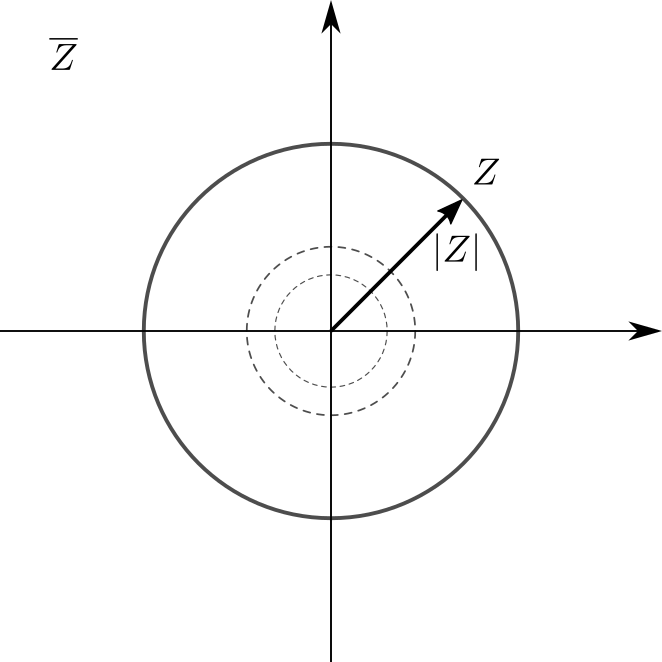
\includegraphics[width=0.35\textwidth]{clase_de_z_complejo.png}
            \caption{Clases de $z$, con $z \in \mathbb{C}$.}
        \end{figure}

    \item Sean $X = \{ a,b,c,d\}$ y 
        $\mathcal{R} = \{ (a,b), (b,b), (c,c), (d,d), (a,b), (b,a) \}$
        
        \nota{Notemos que $\overline{a}$ cubre el par $(a,a)$ y $(b,b)$
        pues $a$ y $b$ se relacionan: $(a,b)$ y $(b,a)$}%
        \[ \nicefrac{X}{\mathcal{R}} = \{ \overline{a}, \overline{c},
        \overline{d} \}\]

        \item ¿Cuántas relaciones de equivalencia se pueden definir en 
            $A = \{1,2,3\}$?

        Contamos las particiones: 

        Si la partición tiene 3 conjuntos, entonces hay una única partición; 
        si hay un único conjunto, es un caso trivial y tendremos también una
        única partición. 

        El caso restante es tener dos conjuntos, en esta situación un conjunto 
        tendrá un único elemento y otro va a tener dos, con lo cual tendremos 
        $\binom{3}{1} = 3$ particiones.

        Por lo tanto, se pueden definir 5 relaciones de equivalencia.
\end{enumerate}



\section{Operaciones en anillos}

Tenemos las siguientes operaciones definidas en $Z_n$:

\begin{itemize}
    \item $\overline{a} + \overline{b} = \overline{a+b}$
    \item $\overline{a} \cdot \overline{b} = \overline{a \cdot b}$
\end{itemize}

\section{Funciones}

\begin{definicion}{Función}{}
    Sean $A$ y $B$ conjuntos.

    Una función de $A$ en $B$ \nota{$f: A \to B$} es una relación $\mathcal{R}
    \subseteq A \times B$ que verifica:

    \begin{gather*}
        \forall x \in A,
        ~ \exists ! \, y \in B
        / (x,y) \in \mathcal{R} \notamath{$A$: Dominio\\ $B$: Codominio}
    \end{gather*}

    \bigskip
    \textbf{Notación:} $y = f(x)$
\end{definicion}

\subsubsection{Ejemplos}
\begin{enumerate}
    \item $\mathcal{R} = \{(x,y) \in \mathbb{R}^2 / y = x\}$ es una función 
        $f: \mathbb{R} \to \mathbb{R}, f(x) = x$. 
        \nota{Esta es la función identidad}%

    \item $\mathcal{R} = \{ (x,y) \in \mathbb{Z}^2 / \divides{x}{y} \}$ no es
        función pues no hay una única imagen:

        \begin{center}
          \begin{tabular}{c c c}
              $(2,4) \in \mathbb{R}$ & $(2,8) \in \mathbb{R}$ & pero $4 \neq 8$
          \end{tabular}
        \end{center}
    \item $\mathcal{R} = \{ (x,y) \in \mathbb{R} \times \mathbb{N} / x = y\}$
        no es función pues: 
        \begin{gather*}
            \sqrt{2} \notin Dom(\mathcal{R})
        \end{gather*}

    \item $\mathcal{R} = \{(x,y,z) \in 
        \underbrace{\mathbb{R}^3}_{\mathbb{R}^2 \times \mathbb{R}} / 
        x^2 + y^2 + z = 0\}$ es función.
        
        \begin{gather*}
            f: \mathbb{R}^2 \to \mathbb{R}, \; f(x,y) = -x^2 - y^2
        \end{gather*}

    \item $\mathcal{R} = \{ (x,y,z) \in \mathbb{R}^3 / x^2 + y^2 + z^2 = 1 \}$
        no es función.

        \begin{center}
            \begin{tabular}{c c c}
                $(0,0,1) \in \mathbb{R}$ & $(0,0,-1) \in \mathbb{R}$ & 
                pero $1 \neq -1$
            \end{tabular}
        \end{center}
\end{enumerate}

\bigskip
\textit{Observación:} 
Sean $A_1, \dotsc, A_n$ conjuntos, 
$\mathcal{R} \subseteq A_1 \times \dots \times A_n$ relación n-aria.

Se puede pensar a $\mathcal{R}$ como una relación binaria: 
$\mathcal{R} \subseteq A \times B$ donde $A = A_1 \times \dots A_{n-1}$ y 
$B = A_n$.

Diremos que $\mathcal{R}$ es una función de $n-1$ variables si 
$\mathcal{R} \subseteq A \times B$, $A$ es el producto cartesiano de $n-1$ 
conjuntos y $\mathcal{R}$ es función.

Es decir, 
    \begin{center}
        $\forall x \in A \; \exists ! \, y \in B / (x,y) \in \mathcal{R}$

        $\iff$

        $\forall (x_1, \dotsc, x_{n-1}) \in A = A_1 \times \dots \times A_{n-1}
        \; \exists ! \, y=x_n \in A_n = B / (x_1, \dotsc, x_n) \in \mathcal{R}$
    \end{center}


\subsection{Clasificación de funciones}

Sea $f: A \to B$ una función.

\begin{itemize}
    \item $f$ es inyectiva si $f(x) = f(y) \implies x = y$
    \item $f$ es sobreyectiva si $\forall y \in B$  $\exists \, x \in A / f(x)=y$
        \nota{Es decir, $Im(f) = B$}%
    \item $f$ es biyectiva si es inyectiva y sobreyectiva.
\end{itemize}

\subsubsection{Ejemplos}

\begin{enumerate}
    \item $f: \mathbb{R} \to \mathbb{R} / f(x) = x^3$
        \begin{itemize}
            \item Inyectiva:

                \begin{gather*}
                    f(x) = f(y) \implies x^3 = y^3 \implies \sqrt[3]{x^3}
                    = \sqrt[3]{y^3} \implies x = y
                \end{gather*}

            \item Sobreyectiva:
                Sea $y \in \mathbb{R}$, busco $x \in \mathbb{R} /f(x)=y$.

                Tomo $x = \sqrt[3]{y}$

                \begin{gather*}
                    \implies f(x) = {\left(\sqrt[3]{y} \right)}^3 = y
                \end{gather*}

            \item Biyectiva: Como $f$ es inyectiva y sobreyectiva, entonces 
                $f$ es biyectiva.
        \end{itemize}

    \item $f: \mathbb{C} \to \mathbb{C} / f(z) = z^3$

        \begin{itemize}
            \item Inyectiva: No es inyectiva.

                Supongamos que $z \in \mathbb{C} / z^3 = 1 \iff z^3-1 = 0$.
                Notemos que esto es un polinomio de grado 3, y, por el teorema
                fundamental del álgebra (TFA), existen 3 raíces del polinomio
                $x^3-1$ en $\mathbb{C}$
                \nota{$(x-1)^3 \neq x^3 -1$}%

                Como hay al menos 2 raíces distintas, entonces existen $z_1$,
                $z_2$, tal que $f(z_1) = f(z_2) = 1 \implies$ no es inyectiva.

                Otra forma es notar que $f(1) = 1$ y también 
                
                \[ f \left(\cos{\left(\frac{2}{3} \pi \right)} 
                    + i \sin{\left(\frac{2}{3} \pi\right)}\right) =
                \cos{\left(3 \; . \; \frac{2}{3} \pi\right)} 
            + i \sin{\left(3 \; . \; \frac{2}{3} \pi\right)} = 1 \]

            \item Sobreyectiva: Tarea.

            \item Biyectiva: Como no es inyectiva, tampoco es biyectiva. 
        \end{itemize}
\end{enumerate}


\subsection{Extensión y restricción de funciones}

\begin{definicion}{Extensión de una función}{}
    Sea $f: A \to B$ una función. 

    Sea $C$ un conjunto tal que $A \subseteq C$ y $D$ un conjunto tal que 
    $D \subseteq B$.

    \medskip
    
    \nota{Defino la función $\tilde{f}$ en un conjunto más grande que $f$, pero 
    ambas coinciden sobre $A$.}%
    Entonces la función $\tilde{f}: C \to D$ es una extensión de $f$ si 
    $\frest{\tilde{f}}{A} = f$, es decir, 
    $\tilde{f}(a) = f(a)$, $\forall a \in A$

\end{definicion}

\bigskip
La restricción de $f$ a $A$ queda entonces definida como:

\begin{definicion}{Restricción de una función}{}
    Sea $f: A \to B$ una función. 

    \medskip

    \begin{center}
        $\frest{\tilde{f}}{A}: A \to B$ es una función tal que 
        $\frest{\tilde{f}}{A} (x) = f(x)$, $\forall x \in A$
    \end{center}
\end{definicion}

\subsubsection{Ejemplos}

\begin{enumerate}
    \item Hallar extensiones a $\mathbb{R}$ de $f: \mathbb{R}_{\geq 0} \to 
        \mathbb{R} / f(x) = x$
        \nota{Pedir una ``extensión a $\mathbb{R}$'' es pedir que el dominio
        de la función extendida sea $\mathbb{R}$.}%

        \begin{enumerate}
            \item $\tilde{f}_1 : \mathbb{R} \to \mathbb{R} / \tilde{f}_1(x)=x$
            \item $\tilde{f}_2 : \mathbb{R}\to\mathbb{R} / \tilde{f}_2(x)=|x|$

                También es una extensión porque si nos restringimos a los 
                $x \geq 0$, tenemos que $|x| = \underbrace{x}_{f(x)}$

            \item $\tilde{f}_3: \mathbb{R}\to\mathbb{R}/\tilde{f}_3(x)=
                \begin{cases}
                    \overbrace{x}^{f(x)} & \text{si } x \geq 0 \\
                    2 & \text{si } x<0
                \end{cases}$

        \end{enumerate}
    Notar que hay infinitas extensiones con distintas propiedades.
    
    Por ejemplo, $\tilde{f}_1$ es continua y derivable, $\tilde{f}_2$
    es continua y no derivable, y $\tilde{f}_3$ no es continua.

    \item Hallar extensiones a $\mathbb{R}$ de $f: \mathbb{R}-\{0\} \to
        \mathbb{R} / f(x) = \frac{\sin{(x)}}{x}$. ¿Existe alguna extensión
        continua?

        \begin{enumerate}
            \item $\tilde{f}_1: \mathbb{R}\to\mathbb{R} / \tilde{f}_1 (x) =
                \begin{cases}
                    \frac{\sin{(x)}}{x} & x \neq 0 \\
                    7 & x = 0
                \end{cases}$

            \item Supongamos que $\tilde{f}$ es una extensión continua. 
                \begin{align*}
                    \implies &\underbrace{\lim_{x\to 0} f(x)} = \tilde{f}(0)\\
                             &\lim_{x\to 0} f(x) = 1
                \end{align*}

                Entonces existe una única extensión continua:
                \[\tilde{f}(x) = \begin{cases}
                    \frac{\sin{(x)}}{x} & x \neq 0 \\
                    1 & x = 0
                \end{cases}\]
        \end{enumerate}

    \item Hallar extensiones a $\mathbb{R}$ de $f: \mathbb{R}-\{0\} \to
        \mathbb{R} / f(x) = \frac{1}{x}$. ¿Existe alguna extensión continua?

        \begin{gather*}
            \notamath{Para algún $a\in\mathbb{R}$}
            \tilde{f}: \mathbb{R}\to\mathbb{R} / f(x) = 
            \begin{cases}
                \frac{1}{x} & x \neq 0\\
                a & x = 0 
            \end{cases}
        \end{gather*}

        Si existe una extensión continua $\tilde{f}$,
        \begin{align*}
            \implies &\underbrace{\lim_{x \to 0} \; f(x)} = \tilde{f}(0)\\
                = & \lim_{x\to 0} \; \frac{1}{x} = \infty 
        \end{align*}

        \begin{gather*}
            \therefore \; \nexists \text{ extensión continua}
        \end{gather*}
\end{enumerate}

\section{Números complejos}

Recordemos que un número complejo $z \in \mathbb{C}: z = a + i b$ puede ser
escrito de la siguiente manera:
\begin{gather*}
    z = e^{i\beta} = \cos{(\beta)} + i \sin{(\beta)}
\end{gather*}

\subsection{Conjunto Gn}

\begin{definicion}{Conjunto $G_n$}{}

    \begin{gather*}
        G_n = \{ z \in \mathbb{C} / z^n = 1 \} 
        = \{ z=e^{i\frac{2k\pi}{n}}, \; k = 0, \dotsc, n-1 \}
    \end{gather*}

\end{definicion}



\section{Transformaciones lineales}

\begin{definicion}{Transformación lineal}{}
    Sean $V$ y $W$ espacios vectoriales.

    \medskip

    Se dice que $T: V \to W$ es una transformación lineal (T.L.) si:

    \begin{enumerate}
        \item $T(u+v) = T(u) +T(v), \quad \forall u,v \in V$ 
        \item $T(\alpha u) = \alpha T(u), \quad \forall u \in V, 
            \forall \alpha \in K$
    \end{enumerate}
\end{definicion}


\subsubsection{Ejemplo}

\begin{itemize}
    \item Sea $T: \mathbb{R}^2 \to \mathbb{R} / T(x,y) = 3x-2y$. Verificar si
        $T$ es una transformación lineal.

        \begin{enumerate}
            \item Sean $u = (x_1, y_1)$ y $v = (x_2, y_2)$.

                \begin{align*}
                    T(u+v) = T(x_1 + x_2, y_1 + y_2) &= \\
                    &= 3(x_1 + x_2) - 2 (y_1 + y_2) \\
                    &= 3 x_1 - 2 y_1 + 3x_2 - 2 y_2 \\
                    &= T(x_1, y_1) + T(x_2, y_2) \\
                    &= T(u) + T(v)
                \end{align*}

            \item Sea $\alpha \in \mathbb{R}$
                \begin{align*}
                    T(\alpha u) = T(\alpha x_1, \alpha y_2) &= \\
                    &= 3 \alpha x_1 - 2 \alpha y_2 \\
                    &= \alpha (3x_1 - 2y_1) \\
                    &= \alpha T(u)
                \end{align*}
        \end{enumerate}

        Por lo tanto, $T$ es una T.L.

    \item Sea $T: \mathbb{R}^2 \to \mathbb{R}^3 / T(x,y) = (x^2,1,2y)$.
        Decidir si $T$ es una T.L.

        Tomemos $u = (1,2)$ y $v=(0,5)$.

        \begin{enumerate}
            \item $T(u+v) = T(1,7) = (1,1,14)$
            \item $T(u)+ T(v) = T(1,2) + T(0,5) = (1,1,4)+(0,1,10)=(1,2,14)$
        \end{enumerate}

        Por lo tanto, $T$ no es T.L.
\end{itemize}

\begin{definicion}{Base}{}
    Una base de un espacio vectorial $V$ es un conjunto 
    $\{ v_1, \dotsc, v_n \}$ 
    tal que:
    \begin{itemize}
        \item El conjunto es linealmente independiente
        \item Genera $V$
    \end{itemize}
\end{definicion}

\begin{teorema}{}{base-tl}
    Sean $v, w$ un $K\mathrm{-}ev$. 

    Sea $B=\{ v_1, \dotsc, v_n \}$ una base
    de $V$ y $\{ w_1, \dotsc, w_n \} \subseteq W$.

    \medskip

    Entonces existe una única transformación lineal de la forma:
    \begin{gather*}
        T \, . \, V \to W / T(v_i) = w_i
        \notamath{$i = 1, \dotsc, n$}
    \end{gather*}
    
\end{teorema}

\subsubsection{Ejemplos}

\begin{itemize}
    \item Consideremos $V = W = \mathbb{R}^2$.

Hallar $\tilde{f} : V \to W$ que extienda a $f$ dada por:
\begin{itemize}
    \item $f(1,0)=(4,-1)$
    \item $f(1,1)=(0,4)$
\end{itemize}


Propongo
\begin{gather*}
    \tilde{f}(x,y) = 
    \begin{cases}
         (4,-1) & \text{si }(x,y)=(1,0) \\
         (0,4) & \text{si } (x,y) = (1,1) \\
         (0,0) & \text{en otro caso}
    \end{cases}
\end{gather*}

\textit{¿Existe alguna extensión que sea T.L.?}

La respuesta es que sí, por el Teorema \ref{teo:base-tl}.

Como $B=\{ (1,0); (1,1) \}$ es base de $\mathbb{R}^2$

\begin{gather*}
    \implies \forall (x,y) \in \mathbb{R}^2, \exists ! \; \alpha, \beta
    \in \mathbb{R} / (x,y) = \alpha(1,0) + \beta (1,1)
\end{gather*}

Encontremos $\alpha$ y $\beta$.

\begin{gather*}
    \begin{cases}
        x = \alpha + \beta \implies \alpha = x -\beta\implies
        \dashbox{$\alpha = x - y$} \\
        \dashbox{$y = \beta$}
    \end{cases}
\end{gather*}

Entonces

\begin{align*}
    \tilde{f}(x,y) = \tilde{f} (\alpha(1,0)+\beta(1,1)) &=\\
    &= \alpha \tilde{f}(1,0) + \beta\tilde{f}(1,1)
    \notamath{Queremos $f$ T.L.} \\
    &= \alpha (4,-1) + \beta (0,4) \\
    &= (x-y)(4,-1) + y(0,4) \\
    &= ( 4(x-y), -(x-y)+4y )
\end{align*}

\begin{gather*}
    \therefore \quad \tilde{f}(x,y) = \left(4x-4y, 5y - x\right)
\end{gather*}

\item Conseguir una TL de $T: \mathbb{R}_2[x] \to \mathbb{R}^3$ tal que
    $T(1+x) = (2,0,0)$

    \medskip

    \nota{$B$ es base pues son 3 elementos LI en un espacio de dimensión 3.}%
    \textit{Plan:} conseguir una base $B = \{ 1+x, 1, x^2 \}$
    y después usar el Teorema \ref{teo:base-tl} para extender a todo 
    $\mathbb{R}_2[x]$.

    Propongamos
    \begin{gather*}
        \circled{$\star$}
        \begin{cases}
            T(1+x) = (2,0,0) \\
            T(1) = (\pi, e, 0) \\
            T(x^2) = (0,0,0)
        \end{cases}
    \end{gather*}

    Usando el Teorema \ref{teo:base-tl}: existe una única
    $T: \mathbb{R}_2[x] \to \mathbb{R}^3$
    y, porque extiende a \circled{$\star$} $\implies$
    $T(1+x) = (2,0,0)$
\end{itemize}

%% Copyright (c) 2022 Martín E. Zahnd
%%
%% This code is licensed under MIT license (see LICENSE.txt for details)
%%
\chapter{Cardinalidad}
\graphicspath{ {./teoria/resources/cardinalidad/} }

\section{Coordinable}

\begin{definicion}{Coordinable}{}
    Sean $A$ y $B$ conjuntos no vacíos.

    \medskip

     $A$ es coordinable con $B$ si $\exists \; f: A \to B$ biyectiva.

\bigskip
\textbf{Notación:} $A \sim B$
\end{definicion}



\bigskip
\textit{Observación:} 
La relación de coordinabilidad es una relación de equivalencia. 
Es decir, $A \mathcal{R} B$ si $A \sim B$, entonces $\mathcal{R}$
es de equivalencia.

\begin{proof} Tarea. \nota{Para \circled{T}, recordar que la composición de
biyectivas es biyectiva.}%
\end{proof}

\begin{definicion}{Sección inicial}{}
        Sea $n \in \mathbb{N}_{\geq 1}$.

        Llamamos \textit{sección inicial} al conjunto 
        $I_n = \{1, 2, 3, \dotsc, n\}$ 
\end{definicion}

\subsubsection{Ejemplo}
\begin{center}
    \begin{tabular}{c c c}
        $I_1 = \{1\}$ &
        $I_2 = \{1,2\}$ &
        $I = \{1,2,3\}$
    \end{tabular}
\end{center}

\bigskip
\textit{Observación:} 
$I_n \sim I_m \iff n = m$

\begin{proof}\phantom{.}

    \begin{itemize}
        \item $\impliedby$) 
            Defino $Id : I_n \to I_m / Id(x) = x$ es biyectiva.
            
            $Id(x) = Id(y) \implies x = y \quad \therefore ~ Id$ es inyectiva.
            
            Sea $b \in I_n \implies Id(b) = b \quad \therefore ~ Id$ es 
            sobreyectiva.

            Por lo tanto, $I_n \sim I_m$

        \item $\implies$) $I_n \sim I_m \implies \exists \; f: I_n \to I_m$
            biyectiva.

            Como $f$ es sobreyectiva,
            \nota{$Im(f)$ significa ``imagen de $f$''}%
            $Im(f) = \{ f(1), f(2), \dotsc, f(n) \} = I_m$ y, además, 
            $I_m$ tiene $m$ elementos por definición.

            Como es inyectiva $f(i) \neq f(j)$ si $i \neq j$ $\implies Im(f)$
            tiene $n$ elementos.

            Y al ser conjuntos iguales $\implies n = m$
    \end{itemize}
\end{proof}


\begin{definicion}{Conjunto finito e infinito}{}
    Sea $A$ un conjunto.

    \medskip

    Decimos que $A$ es \textit{finito} si $A = \varnothing$ o 
    $\exists \; k \in \mathbb{N}_{\geq 1} / A \sim I_k$

    Por otra parte, un conjunto es \textit{infinito} si no es finito.
\end{definicion}

\bigskip
\textit{Observación:} 
El conjunto $\mathbb{N}$ es infinito.

\begin{proof}\phantom{.}

    Supongo que $\mathbb{N}$ es finito $\implies \mathbb{N} = \varnothing$ o
    $\exists \; k \in \mathbb{N}_{\geq 1} / \mathbb{N} \sim I_k$

    \begin{enumerate}[%
                labelindent=*,
                style=multiline,
                leftmargin=*,
                align=left,
                leftmargin=2\parindent,
                label=Caso \arabic*)]

        \item $\mathbb{N} = \varnothing$ 

            ¡Absurdo! $3 \in \mathbb{N}$.

        \item $\exists \; k \in \mathbb{N}_{\geq 1} / 
                \mathbb{N} \sim I_k$
            \begin{gather*}
                \implies \exists \; k \in \mathbb{N} \text{ y } 
                \exists \; f: I_k \to \mathbb{N} \text{ biyectiva.} \\
                Im(f) = \{f(1), f(2), \dotsc, f(k)\} \subseteq \mathbb{N}
                \notamath{$f$ es sobreyectiva.}
            \end{gather*}

            \begin{align*}
                M = \max{(Im(f))} & \\
                \implies& M \in \mathbb{N} \\
                \implies& \text{ Sin embargo } 
                M+1 \in \mathbb{N} \text{ y }  
                M + 1 \notin Im(f) 
            \end{align*}

        Absurdo pues $f$ es sobreyectiva.
    \end{enumerate}


    El absurdo vino de suponer que $\mathbb{N}$ es finito. Por lo tanto, 
    $\mathbb{N}$ es infinito.

\end{proof}

\section{Cardinal}

\begin{definicion}{Cardinal}{}
     $Card(\varnothing) = 0$

     $Card(\mathbb{N}) = \aleph_0$ \nota{$\aleph_0$: ``Aleph cero''}%

     $Card(I_k) = k$ \nota{$k$ es un símbolo que coincide con el número $k$ 
                            pero \underline{no} es un número.}%

    \bigskip
    \textbf{Notación:} $Card(A) = \# A = | A |$
\end{definicion}


\medskip

\begin{definicion}{Comparación de cardinales}{}
    Sean $A$ y $B$ conjuntos tales que $\#A=n$ y $\#B=k$

    \begin{enumerate}
        \item Decimos que $n \leq k$ $\iff$ existe $f: A \to B$ inyectiva.
        \item Decimos que $n < k$ $\iff$ $n \leq k$ y $n \neq k$
        \nota{Estamos diciendo que $n<k$ si y sólo si existe una función 
            inyectiva de $A$ en $B$ pero no existe una función biyectiva de 
            $A$ en $B$.}%
        \item Decimos que $n \geq k$ $\iff$ existe $f: A \to B$ sobreyectiva.
        \item Decimos que $n>k$ $\iff$ $n \geq k$ y $n \neq k$
        \item Decimos que $n = k$ $\iff$ existe $f: A \to B$ biyectiva,\\
            \phantom{Decimos que $n = k$ $\iff$} % Hack for alingment (:
            es decir, si $A \sim B$.
    \end{enumerate}
\end{definicion}


\begin{enumerate}
    \item Veamos que está bien definido. 
        \nota{\textit{Noni:} ``Buena definición.''}%
        Es decir, que no depende del representante elegido. 
        
        Si tomo $\widetilde{A}$ y $\widetilde{B}$ conjuntos tales que 
        $\#\widetilde{A} = n$ y $\#\widetilde{B} = k$
        $\implies \exists \; g: \widetilde{A}\to A$ biyectiva y 
        $h:\widetilde{B}\to B$ biyectiva.

        Luego $h^{-1}\circ f \circ g : \widetilde{A} \to \widetilde{B}$ es inyectiva por 
        composición de funciones inyectivas.
    \item Tarea.
    \item Tarea.
\end{enumerate}

\subsection{Propiedad} \label{subsec:prop-card-lqeq}
\begin{gather*}
    \# A \leq \# B \iff \# B \geq \# A \notamath{Con $A, B \neq \varnothing$}
\end{gather*}

Dicho de otra forma, $\exists \; f:A\to B$ inyectiva 
$\iff \exists \; g:B \to A$ sobreyectiva.

\begin{proof}\phantom{.}

    \begin{itemize}
        \item $\implies$) Si $\# A \leq \# B \implies \exists \; f: A \to B$ 
            inyectiva.

            Defino $g: B \to A$  tal que
            \nota{$f$ es inyectiva: no tiene por qué tener inversa.
                En este contexto, $f^{-1}$ es la preimagen.}%
            \begin{gather*}
                g(b) = \begin{cases}
                    f^{-1}(b) & \text{si } b \in Im(f) \\
                    b & \text{si } b \notin Im(f)
                \end{cases} 
            \end{gather*}


            Notemos que $g$ está bien definida pues $f$ es inyectiva.

            \medskip

            Veamos que $g$ es sobreyectiva:

            Sea $a \in A$.
        \begin{gather*}
                f(a) \in Im(f) \subseteq B \\
                \text{ y }
        \end{gather*}
        \begin{align*}
            g\left(f(a)\right)
                &= f^{-1}\left(f(a)\right) \notamath{$f(a) \in Im(f)$}\\
                &= a \notamath{$f$ es inyectiva}
        \end{align*}

    \item $\impliedby$) Si $\# B \geq \# A \implies \exists \; f: B\to A$ 
        sobreyectiva.

        Definamos una función sobreyectiva $g: A \to B /
        g(a) = X_a$, donde 

        $X_a \in \underbrace{f^{-1}(a)}_{\substack{\text{Preimagen }\\
        \text{de } a}}$ 
        \nota{Usamos el axioma de elección.}%

        Veamos que $g$ es inyectiva.

        Si $a \neq b$ entonces:
        \begin{align*}
            f^{-1}(a) \cap f^{-1}(b) = \varnothing \\
            \implies& X_a \neq X_b \\
            \implies& g(a) \neq g(b)
        \end{align*}

        % Definir la función de este modo tiene un problema: 
        % $g^{-1}(a) \neq \varnothing$ pero $g^{-1}(a)$ puede tener más de un
        % elemento. Es decir, no es necesariamente inyectiva.

        % \nota{Para completar esto, habría que utilizar el axioma de elección
        % (lo vemos más adelante).}%
        % Entonces, para solventar este problema, definimos $f(a) =$ un 
        % elemento fijo $g^{-1}(a)$.

        % Luego, 
        % $f(a_1) = f(a_2) \implies b_1 = b_2$ donde $b_1 \in g^{-1}(a_1)$ y
        % $b_2 \in g^{-1}(a_2)$. Que $b_1=b_2$ implica que 
        % $g(b_1) = g(b_2) = a_1$.
        
        % Pero, como $g$ es función, resulta que 
        % $g(b_1) = g(b_2) \implies a_1 = a_2$

        Entonces $g$ es inyectiva.
    \end{itemize}
\end{proof}



\section{Teorema de Bernstein}
\begin{teorema}{Teorema de Bernstein}{bernstein}
Sea $\#A = m$, $\#B = k$.

\begin{gather*}
    \# A \leq \# B \text{ y } \# A \geq \# B \implies \# A = \# B
\end{gather*}
\end{teorema}

Este teorema nos está diciendo que si existe una función inyectiva de $A$ en 
$B$ y una función sobreyectiva de $A$ en $B$ (no necesariamente la misma 
función), entonces existe una función biyectiva de $A$ en $B$.

Utilizando notación matemática, sean $f$ y $g$ funciones tales que 
$f: A\to B$ es inyectiva y $g: A \to B$ es sobreyectiva 
$\implies \exists \; h : A\to B$ biyectiva.

\begin{proof}
    No la vemos. \nota{\textit{Noni:} Está en el libro de Fava.}%
\end{proof}

\bigskip
\textit{Observación:} 
$\leq$ y $\geq$ son relaciones de orden.
\nota{Pista: ``relaciones de orden'' quiere decir que son relaciones que
cumplen R, A y T.}%

\begin{proof} Tarea. \end{proof}


\subsubsection{Ejemplos}

\begin{enumerate}
    \item \( \# \mathbb{N} \overset{?}{=} \# \mathbb{Z} \)

Hagamos un mapeo, definiendo $F: \mathbb{Z} \to \mathbb{N}$
\begin{center}
    \begin{tabular}{c @{\hskip 1cm} c}
        $0 \to 0$ & \phantom{.} \\
        $1 \to 2$ & $-1 \to 1$ \\
        $2 \to 4$ & $-2 \to 3$ \\
        $3 \to 6$ & $-3 \to 5$ \\
        $4 \to 8$ & $-4 \to 7$
    \end{tabular}
\end{center}

Entonces 
\begin{gather*}
    F(x) = \begin{cases}
        2x & x \geq 0 \\
        -2x-1 & x < 0
    \end{cases}
\end{gather*}

\begin{proof}\phantom{.}

Comencemos probando que $F$ es inyectiva.
\begin{itemize}
    \item $x, y \geq 0$
        \begin{gather*}
            F(x) = F(y) \implies 2x = 2y \implies x = y
        \end{gather*}

    \item $x,y < 0$
        \begin{gather*}
            F(x) = F(y) \implies -2x-1 = -2y - 1 \implies x=y
        \end{gather*}

    \item $x \geq 0, y < 0$: $x \neq y$
        \begin{gather*}
            F(x) = 2x \text{ es par y } F(y) = -2y-1 \text{ es impar.} \\
            \therefore ~ F(x) \neq F(y) 
        \end{gather*}

    \item $y \geq 0, x < 0$: $y \neq x$
        \begin{gather*}
            F(x) = -2x-1 \text{ es impar y } F(y) = 2y \text{ es par.} \\
            \therefore ~ F(x) \neq F(y) 
        \end{gather*}
\end{itemize}

De este modo, probamos la inyectividad.

Nos queda probar la sobreyectividad. Para ello, volvemos a separar en casos.

\begin{enumerate}[%
                labelindent=*,
                style=multiline,
                leftmargin=*,
                align=left,
                leftmargin=2\parindent,
                label=Caso \arabic*)]
    \item Sea $b \in \mathbb{N}$ tal que $b$ es par.
        \[  F \underbrace{%
                \left(\nicefrac{b}{2}\right)}_{\in \mathbb{Z}_{\geq 0}}
             = 2 \; . \; \frac{b}{2} = b \]

    \item Sea $b \in \mathbb{N}$ tal que $b$ es impar.
        \[  F \underbrace{\Bigg( \frac%
            {\overbrace{b+1}^{\text{Par}}}{-2} %
            \Bigg)}_{\in \mathbb{Z}_{< 0}} 
            = (-2) \; . \; \left( \frac{b+1}{-2} \right) -1 = b+1-1 = b \]
\end{enumerate}

Así probamos la sobreyectividad.

Por lo tanto, $F$ es biyectiva y, en consecuencia, 
$\# \mathbb{Z} = \#\mathbb{N}$ \nota{$\# \mathbb{Z} = \aleph_0$}%

\end{proof}

\medskip
\item Hallar el cardinal de $X = \{x \in \mathbb{N} / x \text{ es impar}\}$

    Propongamos una función $F: \mathbb{N} \to X/ F(n) = 2n+1$
    \begin{center}
        \begin{tabular}{c}
            $0 \to 1$ \\ $1 \to 3$ \\ $2 \to 5$ \\ $3 \to 7$
        \end{tabular}
    \end{center}

\begin{proof}\phantom{.}
    \begin{itemize}
        \item Iny.) $F(n) = F(k) \implies 2n+1 = 2k+1 \implies n = k$
        \item Sobrey.) Sea $b \in X$, siendo $b$ impar y $b \geq 1$ y $b-1$ par
            para $b\geq 0$.

            Así, $\frac{b-1}{2} \in \mathbb{N}$, con lo cual 
            $F\left(\frac{b-1}{2}\right) = 2\; . \; \left(\frac{b-1}{2}\right)
            + 1 = b$
        \item Biy.) Como es inyectiva y sobreyectiva, entonces es biyectiva.
    \end{itemize}
    \begin{gather*}
        \therefore ~ \#X=\#\mathbb{N} = \aleph_0
    \end{gather*}

\end{proof}


\item Supongamos que $A \sim \mathbb{N}$, y $B \sim \mathbb{N}$.
        ¿A qué es igual $\# (A\times B)$?

Como $A \sim \mathbb{N}$, $\exists \; f: A\to\mathbb{N}$ biyectiva.
Y como $B\sim\mathbb{N}$, $\exists \; g: B\to\mathbb{N}$ biyectiva.

Definamos $H: A \times B \to \mathbb{N}\times\mathbb{N}$ tal que 
$H(a,b) = \left(f(a), g(b)\right)$.

\begin{proof}\phantom{.}

    \begin{itemize}
        \item Iny.) $H(a,b) = H(x,y)$ 
            \begin{align*}
                \implies& \left(f(a),g(b)\right) = \left(f(x),g(x)\right) \\
                \implies& \underbrace{f(a) = f(x)}_{a=x} ~ \text{ y } ~ 
                \underbrace{g(b) = g(y)}_{b=y} \\
                \implies& (a,b)=(x,y)
            \end{align*}

        \item Sobrey.) Sea $(z_1, z_2) \in \mathbb{N}\times\mathbb{N}$.

        Como $f$ es sobreyectiva $\implies \exists \; a \in A/ f(a) = z_1$,
        y como $g$ es sobreyectiva $\exists \; b \in B/g(b)=z_2$
        \begin{gather*}
            \therefore ~ H(a,b) = \left(f(a),g(b)\right)=(z_1,z_2)
        \end{gather*}

        \item Biy.) Como es inyectiva y sobreyectiva, entonces es biyectiva.
    \end{itemize}
    \begin{gather*}
        \therefore ~  \#(A\times B)=\#( \mathbb{N} \times \mathbb{N})
    \end{gather*}

    Ahora aparece la pregunta, ¿cuál es el cardinal de 
    $\mathbb{N}\times\mathbb{N}$?

\textbf{Diagonales de Cantor}

    \begin{equation*}
        \begin{matrix*}
            (0,0) & (0,1) & (0,2) & (0,3) & (0,4) & (0,5) & \dots \\
            (1,0) & (1,1) & (1,2) & (1,3) & (1,4) & (1,5) & \dots \\
            (2,0) & (2,1) & (2,2) & (2,3) & (2,4) & (2,7) & \dots \\
            (3,0) & (3,1) & (3,2) & (3,3) & (3,4) & (3,5) & \dots \\
            \vdots
        \end{matrix*}
    \end{equation*}
    \[ \mathbb{N}\times\mathbb{N} 
    = \{(x,y) / x \in \mathbb{N}, y \in \mathbb{N}\} \]

    La idea de Cantor fue recorrer todas las tuplas del siguiente modo:
    \begin{figure}[H]
        \centering
        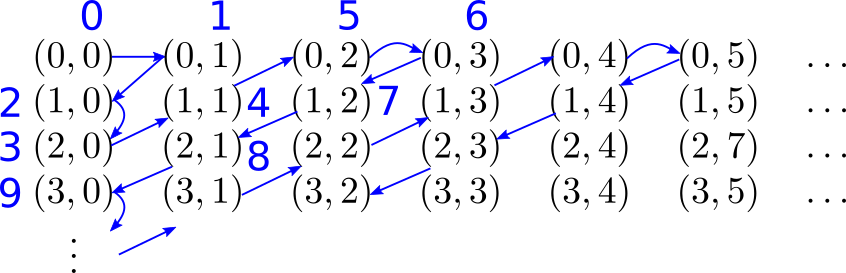
\includegraphics[width=0.70\textwidth]{mapeo_n2yn}
        \caption{Diagonalización de Cantor}
    \end{figure}

    \textit{Noni:} ``Encontrar la fórmula de la función que refleja esto lleva 
    tiempo. Pero la pueden buscar.''

    Hasta acá, obtuvimos que 
    \[ \therefore ~  \#(A\times B)=\#( \mathbb{N} \times \mathbb{N}) =
    \aleph_0 \]

    Pero faltaría probarlo formalmente. 

\end{proof}

\end{enumerate}

\nota{Reescrito con la \fullrefgeneric{subsec:prop-card-lqeq}{%
Propiedad \ref*{subsec:prop-card-lqeq}}}%
\begin{teorema}{Teorema de Bernstein}{bernstein-v2}
Sea $\#A = m$, $\#B = k$.

\[m \leq k \text{ y } k \leq m \implies m = k\]

\end{teorema}

Esto nos dice que teniendo $f: A \to B$ inyectiva y $g: B \to A$ inyectiva,

\begin{gather*}
    \implies \exists \; h: A \to B \text{ biyectiva}
\end{gather*}

La ventaja de este teorema es que trabajamos solamente con funciones 
inyectivas, que son más fáciles de probar que las sobreyectivas.


\begin{proof}
    Usando la \fullrefgeneric{subsec:prop-card-lqeq}{%
    Propiedad \ref*{subsec:prop-card-lqeq}}.
\end{proof}


\subsubsection{Ejemplo}

$\#(\mathbb{N}\times\mathbb{N}) = \aleph_0$
\begin{proof}\phantom{.}
    
    Defino $f: \mathbb{N}\to \mathbb{N} \times \mathbb{N} / f(x) = (x,x)$
    
    $f$ es inyectiva (tarea).
    \begin{gather*}
        \therefore ~ \# \mathbb{N} \leq \# (\mathbb{N} \times \mathbb{N})
    \end{gather*}
    
    Luego, $g: \mathbb{N} \times \mathbb{N} \to \mathbb{N} / g(a,b) = 2^a 3^b$

    \begin{align*}
        g(a,b) = g(c,d) & \\
        \implies& 2^a 3^b = 2^c 3^b \\
        \implies&  a = c \wedge b = d 
        \notamath{Por Teorema Fundamental de la Aritmética (TFA)}
    \end{align*}
    
    Entonces, $g$ es inyectiva y
    $\# (\mathbb{N} \times \mathbb{N}) \leq \mathbb{N}$.
    
    Por el \nameref{teo:bernstein}, 
    $\# \mathbb{N} = \# (\mathbb{N} \times \mathbb{N})$

\end{proof}

\bigskip
\textit{Observación:}
\begin{enumerate}
    \item Cualquier subconjunto de una sección inicial es finito. 

     Es decir, si $A \subseteq I_n \implies A$ es finito.
    \item Si $A \subseteq B$ y $A$ es infinito $\implies B$ es infinito.
\end{enumerate}


\begin{enumerate}
    
    
    \item \begin{proof} Tarea. \nota{\textit{Noni:} ``Recomendación: hacer al 
            finalizar la  teoría de cardinalidad.''}%
    \end{proof}
    \item \begin{proof} \phantom{.}

            Suponiendo que $B$ es finito tenemos dos casos:
            \begin{enumerate}
                \item $B = \varnothing$
                \item $B \sim I_k$ para algún $k \in \mathbb{N}_{\geq 1}$
            \end{enumerate}

            Analicemos cada uno:
            \begin{enumerate}
                \item $A \subseteq B = \varnothing \implies A = \varnothing$
                    $\implies A$ es finito. ¡Absurdo!
                \item $\exists k \in \mathbb{N}_{\geq 1} / 
                    A \subseteq B \sim I_k$

                    \nota{La función inclusión es inyectiva (tarea)}%
                    Por un lado, tenemos la función inclusión: 
                    $inc: A \to B/ inc(a) = a$ 

                    Por otro lado, como
                    $B \sim I_k \implies \exists g: B \to I_k$ biyectiva.

                    \smallskip

                    ¿Qué pasa si componemos $g$ e $inc$?
                    Llamando $h$ a esta función, resulta que
                    $h = g \circ inc: A \to I_k$ es inyectiva por composición
                    de funciones inyectivas.

                    Definamos otra función $\tilde{h}$:

                    \[\tilde{h}: A \to Im(h) \subseteq I_k/\tilde{h}(a)=h(a)\]

                    Notemos que $h$ y $\tilde{h}$ son funciones distintas pues
                    su codominio es diferente.

                    Pero $\tilde{h}$ es biyectiva por ser inyectiva:

                    \begin{gather*}
                        \tilde{h}(a) = \tilde{h}(b) 
                        \implies h(a) = h(b) \implies a = b
                    \end{gather*}

                    Y sobreyectiva:

                    Sea $b \in Im(h)$
                    \begin{align*}
                        &\implies \exists \; a \in A / h(a) = b \\
                        &\implies \tilde{h}(a) = h(a) = b
                    \end{align*}

                    \medskip

                    Por lo tanto, por ser $\tilde{h}$ biyectiva,
                    $\#A = \#Im(h)$
                    y 
                    $Im(h) \subseteq I_k$

                $\underbrace{\implies}_{\substack{\text{Por el item 1}\\%
                \text{ de la observación}}} %
                Im(h)$ es finita
                $\implies$ 
                $A$ es finito. ¡Absurdo!
            \end{enumerate}

            Como el absurdo vino de suponer $B$ finito, entonces $B$ es
            infinito.

        \end{proof}
\end{enumerate}

\bigskip
\textit{Observación:} 
Si $X$ infinito $\implies \exists\; f:\mathbb{N}\to X$ inyectiva.

\medskip

Esta observación nos está diciendo que $\aleph_0 = \# \mathbb{N} \leq \# X$,
es decir, el cardinal más chico de los conjuntos infinitos es $\aleph_0$

\begin{proof}\phantom{.}

    Como $X$ es infinito $\implies X \neq \varnothing \implies \exists \;
    x_0 \in X$.

    Defino $f(0) = x_0$

    \medskip
    Como $X \neq \{x_0\} \sim I_1$ y $X$ es infinito $\implies$ 
    $\exists \; x_1 \in X - \{ x_0 \}$. 

    Defino $f(1) = x_1 \neq x_0$

    Notemos que si
    $X - \{ x_0 \}$ fuera finito 
    $\implies \overbrace{(X-\{x_0\})}^{\text{finito}}
    \cup \overbrace{\{ x_0 \}}^{\text{finito}} = X $ sería finito, lo cual
    es absurdo.
    \nota{Por el ejercicio 3 de la práctica.}%

    \medskip

    Luego $X \neq \{x_0, x_1\} \sim I_2$ y $X$ es infinito $\implies$ 
    $\exists \; x_2 \in X - \{x_0, x_1\}$. 

    Defino $f(2) = x_2$

    Inductivamente,
    $X \neq \{\overbrace{x_0}^{f(0)}, \overbrace{x_1}^{f(1)}, \dotsc, 
    \overbrace{x_n}^{f(n)}\} 
    \sim I_{n+1}$ y $X$ es infinito $\implies$ existe 
    $x_{n+1} \in X - \{f(0), f(1), \dotsc, f(n)\}$. 

    Defino 
    $f(n+1) = x_{n+1} \notin \{ x_0, x_1, \dotsc, x_n \}$


    Y así scesivamente.


    Por último, como cada nueva imagen la elijo en un conjunto donde no están 
    las imágenes anteriores, por definición, $f$ es inyectiva.

\end{proof}


\bigskip
\textit{Observación:}
$A \subseteq B \implies \# A \leq \# B$


\begin{proof} \phantom{.}

    Defino $f: A \to B / f(x) = x$.
    \begin{gather*}
        f(x) = f(y) \implies x = y \\
        \therefore ~ f \text{ es inyectiva}
    \end{gather*}

    Entonces $\# A \leq \# B$.

\end{proof}

\section{Numerable}
\begin{definicion}{Numerable}{}
    \nota{$\# A \leq \mathbb{N}$}%
    $A$ es numerable si $A$ es finito o $A \sim \mathbb{N}$.
\end{definicion}

\subsection{Propiedades}

\begin{enumerate}
    \item $A$ numerable y $A \neq \varnothing 
        \implies \exists \; f:\mathbb{N} \to A$ sobreyectiva.

    \item Si $\exists \; f: \mathbb{N} \to A$ sobreyectiva $\implies A$ es
        numerable.

    \item Si $A$ y $B$ son conjuntos numerables
        $\implies A \times B$ es numerable.
\end{enumerate}

\medskip 

\begin{enumerate}
    \item \begin{proof} Tarea. \end{proof}
    \item \begin{proof} Tarea. \end{proof}
    \item \begin{proof} \phantom{.}

            Como $A$ y $B$ son numerables $\implies$ existen:
            \begin{itemize}
                \item $f_1: \mathbb{N} \to A$ sobreyectiva.
                \item $f_2: \mathbb{N} \to B$ sobreyectiva.
            \end{itemize}

            Luego 
            $f_1 \times f_2 = F: \mathbb{N} \times \mathbb{N} \to A \times B$
            tal que
            \begin{gather*}
                F(n, m) = \left(f_1(n), f_2(m)\right)
            \end{gather*}

            \medskip

            Veamos que $F$ es sobreyectiva.

            Sea $(a,b) \in A \times B$.

            $f_1$ sobreyectiva $\implies$ existe $n \in \mathbb{N}$
            tal que $f_1(n) = a$

            $f_2$ sobreyectiva $\implies$ existe $m \in \mathbb{N}$
            tal que $f_2(m) = b$

            Entonces
            \begin{align*}
                F(n, m) &= \left(f_1(n), f_2(m)\right) = (a,b) \\
                \implies& F \text{ es sobreyectiva} \\
                \implies& \# (
                \underbrace{\mathbb{N} \times \mathbb{N}}_{\aleph_0}
                ) 
                \geq \# (A \times B)
            \end{align*}

            Por lo tanto, $A \times B$ es numerable.
    \end{proof}
\end{enumerate}

\section{Sucesión}

\begin{definicion}{Sucesión}{}
    Una función $f: \mathbb{N} \to A$ es una sucesión de elementos de $A$.

    \bigskip
    \textbf{Notación:} $\left(a_n\right)_{n \in \mathbb{N}}$

    \medskip
    \phantom{\textbf{Notación:}} $\underbrace{f(0)}_{a_0},
    \underbrace{f(1)}_{a_1}, \underbrace{f(2)}_{a_2},
    \underbrace{f(3)}_{a_3}, \dots$
\end{definicion}

\subsubsection{Ejemplo}

\begin{enumerate}
    \item $\begin{cases}
            a_{n+1} = 2 a_n & n \geq 0\\
            a_0 = 1 &
        \end{cases}$

        \[1,2,4,8,16, \dots\]

    \item $a_n = \frac{1}{2^n}$ \nota{$n \in \mathbb{N}$}%

        \[ 1, \frac{1}{2}, \frac{1}{4}, \frac{1}{8} , \dots \]
\end{enumerate}

\section{Proposición}
\begin{proposicion}{}{}
    \[ [0, 1]  = \{ x \in \mathbb{R} / 0 \leq x \leq 1 \} \]

    Es infinito no numerable.
\end{proposicion}

\begin{proof}\phantom{.}

    \begin{enumerate}
        \item $f: \mathbb{N} \to [0,1] / f(x) = \frac{1}{x+1}$ es inyectiva.
            \nota{Tarea}%
            \begin{align*}
                &\implies \# \mathbb{N} \leq \# [0,1] \\
                &\therefore ~ \# [0,1] \geq \aleph_0
            \end{align*}

        \item Supongo que $[0,1]$ es numerable.
            \begin{align*}
                &\implies [0,1] \sim \mathbb{N} \\
                &\implies \exists \; g:\mathbb{N}\to [0,1] \text{ biyectiva}\\
                &\therefore ~ [0,1] = \{ \underbrace{g(0)}_{x_0}, 
                \underbrace{g(1)}_{x_1}, \underbrace{g(2)}_{x_2}, \dotsc \}
            \end{align*}

            \begin{equation*}
                \begin{matrix}
                    x_0 = 0, & x_{00} & x_{01} & x_{02} & x_{03} & x_{04} 
                            & \dots\\
                    x_1 = 0, & x_{10} & x_{11} & x_{12} & x_{13} & x_{14}
                            & \dots \\
                    x_2 = 0, & x_{20} & x_{21} & x_{22} & x_{23} & x_{24}
                            & \dots \\
                \end{matrix}
            \end{equation*}
            
            Con $x_{ij} \in \{0,1,2,3,4,5,6,7,8,9\}$


            Defino $\begin{matrix} 
                d = 0, & d_0 & d_1 & d_2 & d_3 & d_4 & \dots 
            \end{matrix}$,
            \nota{$d_{j} \in \{0,1,2,3,4,5,6,$ $7,8,9\}$}%

            Como $0 \leq d \leq 1 \implies d \in [0,1]$.
            Pero como $d_0 \neq x_{00} \implies d \neq x_0$, 
            $d_1 \neq x_{11} \implies d \neq x_1$, $\dots$,
            $d_n \neq x_{nn} \implies d \neq x_n$

            \begin{gather*}
                \therefore ~ d \notin \{ x_0, x_1, x_2, \dots \}
            \end{gather*}
            \smallskip

            ¡Lo cual es absurdo! Y este vino de suponer que $[0,1]$ es
            numerable.

            \begin{gather*}
                \therefore ~ [0,1] \text{ no es numerable.}
            \end{gather*}
            \smallskip

            Conclusión, el cardinal del $[0,1] > \aleph_0$, pues es un
            conjunto infinito y no numerable.
    \end{enumerate}
\end{proof}

Esta demostración parece ser correcta \textit{pero} contiene un error.

\nota{Repasar sistemas de numeración de Introducción a la Informática.}%
El mismo es que números como $0,23\widehat{9} = 0,24$ son el mismo número 
pero tienen escritura distinta y los estamos comparando como si fueran 
\Verb+string + (cerca del final de la demostración comparamos \Verb+char+ a 
\Verb+char+ los números, $d_0 \neq x_{00} \implies d \neq x_0$)

\medskip
\textit{\textbf{¿Qué números no tienen escritura única?}}

En base 10, los números que tienen colas de ceros se pueden escribir con colas
de nueves.

Por ejemplo, $0,05\widehat{9} = 0,06\widehat{0}$.

\begin{proof}[Parche de la demostración:] \phantom{.}

    Defino $\begin{matrix} 
        d = 0, & d_0 & d_1 & d_2 & d_3 & d_4 & \dots 
    \end{matrix}$ 
    \nota{$d_{j} \in \{1,2,3,4,5,6,$ $7,8\}$}%

    Notar que, como $d$ no tiene ni ceros ni nueves, entonces su escritura es
    única, y puedo compararlos caracter a caracter (decimal a decimal).

\end{proof}

\begin{definicion}{}{}
    \[ \# [0,1] = \mathfrak{C} \]
\end{definicion}

\subsection{Teorema}

\begin{teorema}{}{inf-nonum-cjto-num}
    \begin{enumerate}
        \item Si $X$ es infinito no numerable y $A$ es numerable 
            $\implies X\cup A \sim X$

        \item Si $X$ es infinito no numerable y $A$ es numerable $\implies$
            $X - A \sim X$
    \end{enumerate}
\end{teorema}

\begin{enumerate}
    \item \begin{proof}\phantom{.}

            Como $X$ es infinito $\implies \exists \; f: \mathbb{N} \to X$
            inyectiva.

            \nota{Notemos que $g: \mathbb{N} \to B$ es biyectiva.}%
            Llamamos $B = Im(f) \sim \mathbb{N}$ y $B \subseteq X$

            Luego, 
            \begin{align*}
                Y = X - B & \\
                &\implies X = Y \cup B \\
                &\implies X \cup A = (Y \cup B) \cup A = Y \cup (B \cup A)
            \end{align*}

            \nota{Por el ejercicio 3 de la guía.}%
            $A$ y $B$ numerables $\implies A \cup B$ es numerable.

            Como $B$ es infinito y $B \subset A \cup B \implies A \cup B$
            infinito.

            Como $A\cup B$ es numerable e infinito, entonces 
            $A\cup B \sim \mathbb{N}$ y $B \sim \mathbb{N}$.
    
            \nota{La relación de coordinabilidad es de equivalencia, y, en
                consecuencia, transitiva.}%
            Por lo tanto, por transitividad , resulta que $A \cup B \sim B$
            \[ X \cup A = Y \cup (\underbrace{B \cup A}_{\sim B}) 
            \sim Y \cup B = X \]

            \[ \therefore ~ X \cup A \sim X \]

            \medskip

            Veamos que $Y \cup (B \cup A)  \sim Y \cup B$

            \begin{enumerate}[%
                labelindent=*,
                style=multiline,
                leftmargin=*,
                align=left,
                leftmargin=2\parindent,
                label=Caso \arabic*)]
                \item $A \cap Y = \varnothing$

                    Sea 
                    $H: Y \cup (B \cup A) \to Y \cup B / H(x) = \begin{cases}
                        x & x \in Y \\
                        f(x) & x \notin Y
                    \end{cases}$

                    Como $B \cup A \sim B$, existe $f: B \cup A \to B$
                    biyectiva.

                    \textit{Tarea:} ver que $H$ es biyectiva.

                \item $A \cap Y \neq \varnothing$

                    Podemos reescribir $A$ como 
                    $A = (A \cap Y) \cup (\overbrace{A - Y}^{\widetilde{A}})$,
                    y como $A$ es numerable, cualquier subconjunto lo es. 
                    En particular $\widetilde{A}$ es numerable.


                    Luego, $X \cup \widetilde{A} = X \cup A$. Con esto caigo en
                    el Caso 1, con $\widetilde{A}$ en lugar de $A$.

                    \begin{gather*}
                        \therefore ~ X \cup \widetilde{A} \sim X
                    \end{gather*}

            \end{enumerate}

    \end{proof}


    \item \begin{proof}\phantom{.}

        \begin{enumerate}[%
                labelindent=*,
                style=multiline,
                leftmargin=*,
                align=left,
                leftmargin=2\parindent,
                label=Caso \arabic*)]
            \item $A \subseteq X$

                Tenemos que $X = (X-A) \cup A$, con $A$ numerable.

                \nota{Por ejercicio 3 de la guía.}%
                Si $X-A$ es numerable $\implies (X-A)\cup A$ es numerable
                $\implies X$ es numerable.

                Lo cual es un absurdo. Por lo tanto, $X-A$ no es numerable.
                Entonces, $X-A$ es infinito no numerable.

                \medskip

                Por la proposición anterior, 
                \begin{gather*}
                    (\underbrace{X-A}_{\text{Inf. no num.}}) \cup
                    \underbrace{A}_{\text{Num.}} \sim X-A
                    \implies X \sim X - A
                \end{gather*}


            \item $A \not\subseteq X \implies A = 
                (\underbrace{A \cap X}_{\widetilde{A}}) \cup (A-X)$

                $X-A=X-\widetilde{A}$ y caigo en el Caso 1 con $\widetilde{A}$ en 
                lugar de $A$. \nota{$\widetilde{A} \subseteq X$}%

        \end{enumerate}
    \end{proof}
\end{enumerate}

\subsubsection{Ejemplos}
\begin{itemize}
    \item $\# (0,1) = \mathfrak{C}$

        \begin{proof}\phantom{.}

            \[ \underbrace{[0,1]}_{\text{Inf. no num.}} 
            - \underbrace{\{0,1\}}_{\text{Finito num.}} \sim [0,1] 
        \implies (0,1) 
        \underbrace{\sim}_{\fullref{teo:inf-nonum-cjto-num}}
        [0,1]\]
        \end{proof}

    \item Analogamente, $(0,1] \sim [0,1]$

    \item $\# (-10, 10) = \mathfrak{C}$

        ¡Sí!

        \begin{proof}\phantom{.}
            Veamos que se puede generalizar como $\# (a, b) = \mathfrak{C}$, 
            con $a, b$ números (ninguno es $\infty$).

        \begin{figure}[H]
            \centering
            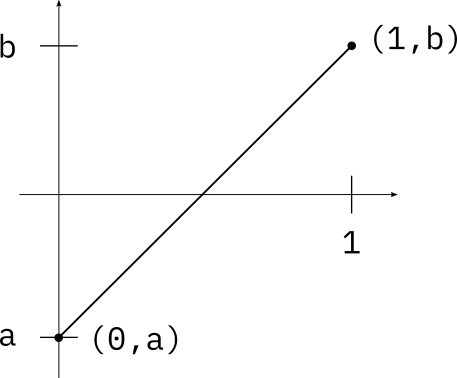
\includegraphics[width=0.45\textwidth]{mapeo_0-1_a-b}
            \caption{$y = (b-a)x + a$}
        \end{figure} \nota{$y=\left(\frac{b-a}{1-0}\right)(x-0)+a$}%

        \[ F: (0,1) \to (a,b) / F(x) = (b-a) x + a \]

        Como $F$ es biyectiva (tarea), entonces $C = \#(0,1) = \#(a,b)$

        \end{proof}

    \item $\# \mathbb{R} = \mathfrak{C}$
        \begin{proof}\phantom{.}
            
            Tomemos la función $\tan{(- \nicefrac{\pi}{2}, \nicefrac{\pi}{2})}
            \to \mathbb{R}$, que es biyectiva.

            Por el item anterior, sabemos que $\# (a,b) = \mathfrak{C}$, 
            entonces:

            \[ \# \left(-\frac{\pi}{2}, \frac{\pi}{2}\right) 
            = \# \mathbb{R} = \mathfrak{C} \]

        \end{proof}
        
        Otra forma de demostrarlo, más analítica es la siguiente:

        \begin{proof}\phantom{.}

            Sea $G: \mathbb{R} \to (-1,1) / G(x) = \frac{x}{1+|x|}$

            Veamos que está bien definida:

            \[ |G(x)| = \left| \frac{x}{1+|x|} \right| 
            = \frac{|x|}{1+|x|} < 1 \iff |x| < 1 + |x| \]

            Para probar que $G$ es biyectiva (tarea), podemos tomar dos 
            caminos:

            \begin{enumerate}
                \item Probar que $G$ es inyectiva y sobreyectiva.
                \item Probar $H: (-1,1) \to \mathbb{R} / 
                    H(x) = \frac{x}{1-|x|}$ es la inversa de $G$
            \end{enumerate}
            
        \end{proof}
\end{itemize}


\section{Teorema de Cantor}

\begin{teorema}{Teorema de Cantor}{cantor}
    Dado $X$ un conjunto, $\# X < \# \mathcal{P}(X)$
\end{teorema}


Este teorema nos está diciendo que:
\[ \# \mathbb{N} = \aleph_0
    < \# \mathcal{P}(\mathbb{N})
    < \# \mathcal{P}(\mathcal{P}(\mathbb{N}))
    < \# \mathcal{P}(\mathcal{P}(\mathcal{P}(\mathbb{N})))
    < \dots \]

Es decir, hay infinitos cardinales distintos correspondientes a conjuntos
infinitos.

\begin{proof} \phantom{.}

    Sea $F: X \to \mathcal{P}(X) / F(a) = \{a\} \subseteq X$
    \begin{gather*}
        F(a) = F(b) \implies \{a\} = \{b\} \implies a = b \\
        \therefore ~ F\text{ es inyectiva.}
    \end{gather*}

    Por esto, $\# X \leq \# \mathcal{P}(X)$

    \nota{Recordar:
    $\#A \geq \#B$
    $\iff$
    $\exists \; f: A \to B$ sobreyectiva}%
    Para ver que es menor estricto, tenemos que ver que no existe ninguna 
    función sobreyectiva de $X$ en $\mathcal{P}(X)$, ya que esto implica
    que no puede ser mayor o igual.

    Supongo que existe $g: X \to \mathcal{P}(X)$ sobreyectiva.

    $B = \{ a \in X / a \notin g(a) \} \subseteq X
    \quad \therefore ~ B \in \mathcal{P}(X)$ 

    \medskip
    Notemos que $g(x)$ ($g$ evaluada en $x$) es un conjunto.

    Por ejemplo, si tuviéramos una función
    $g: \mathbb{N} \to \mathcal{P}(\mathbb{N})$ tal que:
    \begin{gather*}
    g(3) = \{1,2,4\}, \quad g(5) = \{5,6\} \\
    \\
    3 \notin g(3), \; 5 \in g(5) \\ \implies 3 \in B, 5 \notin B
    \end{gather*}

    \medskip

    Como la función $g$ es sobreyectiva $\implies$ existe $b \in X$ tal que
    $g(b) = B$

    Naturalmente surge la pregunta: ¿$b \in B$?.
    \[ b \in B \underbrace{\iff }_{\text{Def. } B} b \notin g(b) 
        \underbrace{\iff}_{g(b)=B} b \notin B \]

    ¡Absurdo! Vino de suponer que existe una $g$ sobreyectiva.
    \begin{align*} 
        \therefore ~ &\nexists \; g:X \to\mathcal{P}(X) \text{ sobreyectiva}\\
        &\implies \# X \not\geq \# \mathcal{P}(X) \\
        &\implies \# X < \# \mathcal{P}(X)
    \end{align*}
\end{proof}

\section{Álgebra de cardinales}

\begin{definicion}{Álgebra de Cardinales}{}
    Sean $a = Card(X)$ y $b = Card(Y)$

    Definimos
    \begin{enumerate}
        \item $a + b = \# (X \cup Y)$, con $X \cap Y = \varnothing$
        \item $a \cdot b = \# (X \times Y)$
        \item $a^b = \# \{ f: Y \to X / f $ es función
            $\} = \# \left({X}^{Y}\right)$
            \nota{$X \neq \varnothing$, $Y \neq \varnothing$}%
    \end{enumerate}

\end{definicion}

\begin{proof} Buena definición.

    \begin{enumerate}
        \item Sea $\underbrace{\widetilde{X} \sim X}_{\# \widetilde{X} = a}$.

            Sea $\underbrace{\widetilde{Y} \sim Y}_{\# \widetilde{Y} = b}$ 
            tal que
            $\widetilde{X} \cap \widetilde{Y} = \varnothing$

            Quiero ver que 
            $\# (\widetilde{X} \cup \widetilde{Y}) = \# (X \cup Y)$

            \begin{align*}
                \widetilde{X} \sim X & \implies \exists \;
                f: \widetilde{X} \to X
                \text{ biyectiva}\\
                \widetilde{Y} \sim Y & \implies \exists \;
                g: \widetilde{Y} \to Y
                \text{ biyectiva}\\
            \end{align*}

            Defino $H: \widetilde{X} \cup \widetilde{Y} \to X \cup Y/$ 
            \nota{Buena definición pues 
            $\widetilde{X}\cap\widetilde{Y}=\varnothing$}%
            $H(z) = \begin{cases}
                f(z) & \text{si } z \in \widetilde{X} \\
                g(z) & \text{si } z \in \widetilde{Y} \\
            \end{cases}$

            Tarea: $H$ es biyectiva.

        \item Defino $m \, . \, n = \# (X \times Y)$

            Tarea: probar la buena definición.

        \item Defino $X \neq \varnothing$, $Y \neq \varnothing$.

            \begin{gather*}
                m^{n} = \# \{ f: Y \to X / f \text{ es función} \} = \# X^{Y}
            \end{gather*}

            Veamos que está bien definida.

            
            % Puesta acá para correcta alineación con la página
            \nota{Notemos que los elementos de ${X}^{Y}$ son funciones de $Y$
                en $X$; y los de ${\widetilde{X}}^{\widetilde{Y}}$ son 
                funciones de $\widetilde{Y}$ en $\widetilde{X}$.}%
            \begin{align*}
                \widetilde{X}\sim X &\implies \exists \; f: \widetilde{X} 
                \to X \text{ biyectiva}  \\
                \widetilde{Y}\sim Y &\implies \exists \; g: \widetilde{Y} 
                \to Y  \text{ biyectiva}
            \end{align*}

            Veamos que ${X}^{Y} \sim {\widetilde{X}}^{\widetilde{Y}}$

           \medskip

             Defino $H: {X}^{Y} \to {\widetilde{X}}^{\widetilde{Y}} / H(F)=G$,
            siendo
            $G(a) = f^{-1} \circ F \circ g(a) \in \widetilde{X}$, con 
            $a \in \widetilde{Y}$

            \begin{itemize}
                \item Inyectividad)
                    \begin{align*}
                        H(F_1) = H(F_2) & \\
                        &\implies G_1 = G_2 \\
                        &\implies G_1(a) = G_2(a)
                        \notamath{$\forall a \in \widetilde{Y}$} \\
                        &\implies f^{-1}\circ F_1 \circ g(a) =
                        f^{-1} \circ F_2 \circ g(a) 
                        \notamath{$\forall a \in \widetilde{Y}$} \\
                        &\implies \underbrace{f \circ f^{-1}}_{id} 
                        \circ F_1 \circ g(a) =
                        \underbrace{f \circ f^{-1}}_{id} 
                        \circ F_2 \circ g(a)
                        \notamath{$f$ es biyectiva. 
                            $\forall a \in \widetilde{Y}$} \\
                        &\implies F_1(g(a)) = F_2(g(a))
                        \notamath{$\forall a \in \widetilde{Y}$}
                    \end{align*}

                    Luego, $F_1, F_2 : Y \to X$

                    Queremos ver que $F_1(y) = F_2(y)$, $\forall y \in Y$

                    Sea $y \in Y \implies \exists z \in \widetilde{Y}/g(z)=y$,
                    pues $g$ es sobreyectiva.

                    Como $F_1(g(a)) = F_2(g(a))$, entonces
                    $F_1(\underbrace{g(z)}_{y}) = F_2(\underbrace{g(z)}_{y})$

                    \begin{gather*}
                        \therefore ~ F_1 = F_2
                    \end{gather*}

                    En conclusión, $H$ es inyectiva.

                \item Sobreyectividad) Tarea.
            \end{itemize}

    \end{enumerate}

\end{proof}

\subsubsection{Ejemplos}
\begin{itemize}
\item \begin{align*}
    2 + 3 &= 
    \# \left(\{\circ, \bigtriangleup\} \cup \{x_1,x_2,x_3\}\right) \\
    & = \# \left(\{\circ, \bigtriangleup, x_1,x_2,x_3\}\right) \\
    &= 5
\end{align*}

\textit{``¡Oh! ¡Qué novedad! ¡$2+3=5$!''} 

Sí, es novedoso porque acá estamos hablando de \textit{cardinales}.
Sus símbolos coinciden con los de los números, pero no significan lo
mismo.

La ventaja es que si los símbolos coinciden con los de los números,
su suma también lo hace.

\item $\# \{ \mathbb{N} \to \{-1,1\} / f \text{ es función} \} 
    = {(\#\{-1,1\})}^{\mathbb{N}} = 2^{\aleph_0}$

    \item $\# (\mathbb{N}\times\mathbb{N}) =  \mathbb{N} \cdot \mathbb{N} 
        = \aleph_0 \cdot \aleph_0$ y, como 
        $\# (\mathbb{N} \times \mathbb{N}) = \# \mathbb{N} = \aleph_0 $, entonces 
        $\aleph_0 \cdot \aleph_0 = \aleph_0$
\end{itemize}

\subsection{Propiedad}
\begin{gather*}
    \# \mathcal{P}(X) = 2^{\# X}
\end{gather*}

% Puesta acá para correcta alineación con la página
\nota{\textit{Noni:} ``En matemática parece un poco extraño, pero en
programación lo hacemos naturalmente: definimos funciones que reciben
cualquier argumento y devuelven otra función.''}%
\begin{proof}\phantom{.}

    Sea $Y = \{f: X \to \{0,1\} / f \text{ es función} \}$, por las
    definiciones vistas anteriormente $\# Y = 2^{\# X}$

    $F: \underbrace{\mathcal{P}(X)}_{\text{Conjuntos}} 
    \to \underbrace{Y}_{\text{Funciones}} / 
    F(\text{conjunto}) = \text{función}$

    \medskip

    Definamos $F(A) = \Chi_A$

    \begin{itemize}
        \item Iny.) 
            % Puesta acá para correcta alineación con la página
            \nota{$\Chi_A$ es la función característica de A.\\
                Recordemos que se define como: \\
            $\Chi_A: X \to \{0,1\}/$ $\Chi_A (t) = \begin{cases}
                1 & t \in A \\ 0 & t \notin A
            \end{cases}$}%
            $F(A) = F(B) \implies \Chi_A = \Chi_B 
            \implies \Chi_A (t) \underbrace{=}_{*} 
            \Chi_B (t) $, $\forall t \in X$
           \begin{align*}
               \text{Sea } t \in A \phantom{\iff} & \\
               \iff &\Chi_A (t) = 1 \\
               \underbrace{\iff}_{*} &\Chi_B (t) = 1 \\
               \iff & t \in B
           \end{align*}
           \begin{gather*}
               \therefore ~  t \in A \iff t \in B
           \end{gather*}

           Entonces $A = B$.
       \item Sobrey.) Sea $h \in Y$.

           Defino $C = \{ x \in X / h(x) = 1 \} \subseteq Y$

           Entonces $C \in \mathcal{P}(x)$ y tiene sentido hacer 
           $F(C) \implies F(C) = \Chi_C$

           \bigskip
           Veamos que $\Chi_C = h$

           Sea $t \in X_C$.
           \begin{align*}
               \Chi_C (t) = 1 & \\
               & \iff t \in C \\
               & \iff h(t) = 1 \notamath{Definición de $C$} \\
            \end{align*}

            Es decir, \dashbox{$\Chi_C (t) = 1 \iff h(t) = 1$}

            Lo cual es equivalente a decir que 
            $\Chi_C (t) \neq 1 \iff h(t)\neq 1$, que a su vez es equivalente a
            $\Chi_C (t) = 0 \iff h(t) = 0$

            \[ \therefore ~ \Chi_C = h \]
    \end{itemize}
    Conclusión, $F$ es biyectiva 
    $\implies \# \mathcal{P}(x) = \# Y = 2^{\# X}$

\end{proof}


\subsection{Teorema}

\begin{teorema}{}{}
    \begin{gather*}
        2^{\aleph_0} = \mathfrak{C}
    \end{gather*}
\end{teorema}

\begin{proof}\phantom{.}

    Sea
    $U = [0,1] \implies \# U = \mathfrak{C}$

    Sea
    $T = {\{0,1\}}^{\mathbb{N}}
    = \{f:\mathbb{N} \to \{0,1\}/f \text{ es función}\}
    \implies \# T=2^{\aleph_0}$


    \nota{Interpreto el número en base 2.}%
    Defino $F: T \to U / F(a_0 a_1 a_2 a_3 \dots) = {(0,a_0 a_1 a_2 a_3 )}_2$

    \begin{gather*}
        a_0 a_1 a_2 a_3 \dots \mapsto \notamath{$(0,1)_2 
                                    = \nicefrac{1}{2} = 0,5$}%
        x = \sum_{k=1}^{\infty} \frac{a_{k-1}}{2^k}
    \end{gather*}

    \begin{align*}
        F(a_0 a_1 a_2 \dots) &= F(b_0 b_1 b_2 \dots)  \\
        &\implies (0, a_0 a_1 a_2 \dots)_2 = (0, b_0 b_1 b_2 \dots)_2 \\
        & \underbrace{\implies}_{\text{Mal}} 
        a_j = b_j \; \forall j \in \mathbb{N} \notamath{Esta 
            implicación está mal porque en base 2 los números no tienen
            escritura única.\\$0,010\widehat{1}=0,011$} \\
        &\implies a_0 a_1 a_2  \dots = b_0 b_1 b_2  \dots
    \end{align*}

    Así como está escrita, $F$ no es inyectiva pues 
    \[F(01011111 \dots) = F(01100000 \dots)\]

    \phantom{.}

    Para arreglar esto, definimos 
    $T_0 = \{ f \in T / f \text{ tiene colas de ceros}\}$, o lo que es lo
    mismo, $T_0 = \{ f \in T / 
    f(x) = 0 ~ \forall k \vee f(k) = 0 ~ \forall k \geq j \text{ y } f(j-1)=1 \}$

    Definimos también
    $G: T_0 \to \mathbb{N} / G(a_0 a_1 \dots a_{j-1} 0 \dots 0) 
    = 1 a_0 a_1 \dots a_{j-1}$

    $G$ es inyectiva:
    \begin{align*}
        G(a_0 a_1 \dots a_{j-1} 0 \dots 0) &= 
        G(b_0 b_1 \dots b_{t-1} 0 \dots 0) \\
        &= 1 a_0 a_1 \dots a_{j-1} = 1 b_0 b_1 \dots b_{t-1} \\
        &\implies a_i = b_i \forall \, i \\
        &\implies G \text{ es inyectiva} \\
        &\implies \# T_0 < \# \mathbb{N} = \aleph_0 \\
        &\implies T_0 \text{ es numerable} \\
        \\
        & \therefore ~ \# (T-T_0) = \# T = 2^{\aleph_0}
        \notamath{ $T-T_0\sim T$\\ Con $T$
            infinito no numerable, pues $2^{\aleph_0} > \aleph_0$ 
        (por el \nameref{teo:cantor}), $T_0$ numerable y, en consecuencia,
        $\# T = 2^{\aleph_0}$. }
    \end{align*}

    \phantom{.}

    Defino ahora $F: (T-T_0) \to U / F(a_0 a_1 \dots a_{j-1} 0 \dots 0)
    = (0, a_0 a_1 \dots )_2 $

    Estos números sí tienen escritura única pues no hay colas de ceros.
    Solucionamos así el problema de la inyectividad.

    \begin{align*}
        F(a_0 a_1 a_2 \dots) &= F(b_0 b_1 b_2 \dots) \\
        &\implies (0, a_0 a_1 a_2 \dots)_2 = (0, b_0 b_1 b_2 \dots)_2 \\
        & \implies
        a_j = b_j \; \forall j \in \mathbb{N} \notamath{Al no tener cola
        de ceros, tienen escritura única} \\
        & \therefore ~ F \text{ es inyectiva}
    \end{align*}

    \[ \dashbox{$\# (T-T_0) \leq \# U$} \]

    Ahora la sobreyectividad.

    Para ella, notamos un problema: al sacar las colas de ceros, también 
    sacamos al cero. En consecuencia, el cero no va a estar en la imagen y
    la función no va a ser sobreyectiva.

    \begin{gather*}
        \widetilde{U} = (0,1] \sim [0,1] - \{ 0 \} \\
        \therefore ~ \# \widetilde{U} = \mathfrak{C}
    \end{gather*}

    Queda entonces definida \nota{Con $\widetilde{U} = (0,1]$}%

    $F: (T-T_0) \to \widetilde{U} / F(a_0 a_1 \dots a_{j-1} 0 \dots 0)
    = (0, a_0 a_1 \dots )_2 $


    Con esto, $F$ es sobreyectiva:

    
    \begin{gather*}
        x \in \widetilde{U} \implies x = (
        \underbrace{0, u_0 u_1 u_2 u_3 u_4 u_5 \dots}_{\substack{
            \text{Lo escribo de forma tal} \\
            \text{que no tenga cola de ceros.}
        }})_2 \notamath{$(0,1)_2 = (0,0\widehat{1})_2$}%
        \\ \\
        \therefore ~ F(u_0 u_1 u_2 \dots) = x
    \end{gather*}

    Conclusión, $F$ es biyectiva y, en consecuencia,
    $\# (T-T_0) = \# \widetilde{U}$.

    Como $\#(T-T_0) = 2^{\aleph_0}$ y $\# \widetilde{U} = \mathfrak{C}$, 
    queda probado que

    \[ \boxed{2^{\aleph_0} = \mathfrak{C}} \]

\end{proof}

\subsubsection{Ejemplo}

Calcular ${\aleph_0}^{\aleph_0}$

\begin{align*}
    2 \leq \aleph_0 \leq C & \\
    &\implies \notamath{Por ej. de la guía}
    2^{\aleph_0} \leq {\aleph_0}^{\aleph_0} 
    \leq {C}^{\aleph_0} = {\left(2^{\aleph_0}\right)}^{\aleph_0} \\
    &\implies \notamath{Por ej. de la guía: 
    $\left(2^x\right)^y = 2^{xy}$}
    2^{\aleph_0} \leq {\aleph_0}^{\aleph_0} \leq 2^{\aleph_0 \cdot \aleph_0}
    = 2^{\aleph_0} \\
    &\implies C \leq {\aleph_0}^{\aleph_0} \leq C \\
    &\implies \boxed{{\aleph_0}^{\aleph_0} = \mathfrak{C}}
\end{align*}

\section{Hipótesis del continuo}

\nota{\textit{Noni:} ``Es una \textit{hipótesis} y no un \textit{teorema} pues
no hay demostración de que este conjunto exista o no, pero la comunidad
matemática acuerda construir sobre esto.''}%
\begin{hipotesis}{Hipótesis del continuo}{}
    \[ \nexists \; X \text{ conjunto tal que } \aleph_0 < \# X < C \]
\end{hipotesis}

La hipótesis está diciendo que no hay ningún conjunto entre $\aleph_0$ y $C$.

\section{Truco visto en la práctica}

\begin{itemize}
    \item En algunos problemas podemos definir 
        \begin{gather*}
            f : A \to B / f(x) = x
        \end{gather*}
        Y demostrar fácilmente que $f$ es inyectiva.
\end{itemize}

%% Copyright (c) 2022 Martín E. Zahnd
%%
%% This code is licensed under MIT license (see LICENSE.txt for details)
%%
\chapter{Lógica Proposicional}\label{chap:logica-proposicional}
% \graphicspath{ {./teoria/resources/logica-proposicional/} }

\section{Lenguajes}
\subsection{Alfabeto}

\begin{definicion}{Alfabeto}{}
    Sea $A$ un conjunto, con $A \neq \varnothing$.

    \medskip

    El conjunto $A$ se llama alfabeto.
\end{definicion}


\subsection{Expresión}

\begin{definicion}{Expresión}{}
    Una expresión es una sucesión finita de elementos de $A$ o la cadena 
    vacía, a la cual llamamos $\lambda$.
\end{definicion}

\subsubsection{Ejemplo}
\begin{gather*}
    A = \{ 1,2,3,5,4,6 \}
\end{gather*}

Las expresiones son: $121$, $4$, $\lambda$, $66666$


\subsection{Longitud}

\begin{definicion}{Longitud}{}
    Sea $E = e_0 e_1 \dots e_{n-1}$ una expresioń de elementos de $A$, 
    definimos:
    \begin{enumerate}
        \item $long(E) = n$
        \item $long(\lambda)=0$
    \end{enumerate}
\end{definicion}

\subsection{Conjunto A estrella}

\begin{definicion}{$A^{*}$}{}
    \begin{gather*}
        A^{*} = \bigcup_{n\in \mathbb{N}} A^n
    \end{gather*}
\end{definicion}

Entonces, en $A^{*}$ están:
\begin{gather*}
    A^0 = \{ \lambda \}, \; \notamath{$\lambda = \text{`` ''}$}
    A^1 = A, \; 
    A^j = \{ e \text{ expresión en } A / long(e) = j \}
\end{gather*}

\bigskip
\textit{Observación:}
$A^{*}$ es infinito.

\begin{proof} \phantom{.}

    Sea $A \neq \varnothing$.

    \begin{align*}
         \implies& \exists x \in A \\
         \implies& x, xx, xxx, xxxx, \dotsc \in A^{*}
    \end{align*}

    Por lo tanto
    \begin{gather*}
        f: \mathbb{N} \to A^{*} / f(n) =
        \begin{cases}
            \lambda & n = 0 \\
            \underbrace{x \, . \, x \, . \, \dotsc \, . \, x}_{n 
        \text{ veces}} & n \geq 1
        \end{cases}
    \end{gather*}

    Y como $f$ es inyectiva $\implies \# A^{*} \geq \aleph_0$
\end{proof}

\subsection{Lenguaje}

\begin{definicion}{}{}
    Dado $A$ un alfabeto.

    \medskip

    \nota{$\Sigma \subseteq A^{*}$}% 
    Un lenguaje $\Sigma$ sobre $A$, con $\Sigma \neq \varnothing$,
    es un subconjunto de $A^{*}$.

\end{definicion}

\subsubsection{Ejemplos}

\begin{enumerate}
    \item $A = \{ a, \dotsc, z \} \implies \# A = 27$

        Entonces definimos el lenguaje como:
        
        \begin{gather*}
            \Sigma \subseteq A^{*} / \Sigma = \{ e \in A^{*} / e 
                \text{ es una palabra que está en la última edición del } \\ 
            \text{diccionario de la Real Academia Española.} \}
        \end{gather*}

    \item Sea $A = \{ 0, 1, 2, 3, 4, 5, 6, 7, 8, 9 \}$.

        \begin{align*}
            \mathcal{L} &= \{ x \in A^{*} / x 
            \text{ representa un número natural} \} \\
              &= \{ x \in A^{*} / x = a_1, \dotsc, a_n, \text{ con }
              a_j \in A \text{ y } a_1 \neq 0\} \cup \{ 0 \}
        \end{align*}
\end{enumerate}

\subsection{Igualdad de expresiones}


\begin{definicion}{Igualdad de expresiones}{}
    Sean las expresiones $E$ y $F$ sobre $A$.

    \medskip

    Entonces $E = F \text{ si } long(E) = long(F)$ y
    \begin{center}
    \begin{enumerate}[%
                    labelindent=*,
                    style=multiline,
                    leftmargin=*,
                    align=left,
                    leftmargin=2\parindent,
                    label=Caso \arabic*)]
        \item $long(E)= 0 \implies E = F = \lambda$
        \item $long(E) = n \implies E = e_0 e_1 \dots e_{n}$ y
            \nota{$0 \leq i \leq n$}%
            $F = f_0 f_1 \dots f_j$, con $n = j$ y $e_i = f_i$.
    \end{enumerate}
    \end{center}
\end{definicion}

\subsection{Concatenación}

\begin{definicion}{Concatenación}{}
    \begin{center}
        \begin{enumerate}[%
                        labelindent=*,
                        style=multiline,
                        leftmargin=*,
                        align=left,
                        leftmargin=2\parindent,
                        label=Caso \arabic*)]
            \item Sean las expresiones $E = e_0 e_1 \dots e_{n-1}$ 
                y 
        $F = f_0 f_1 \dots f_{k-1}$, con $E, F \in A^{*}$

        \medskip

        Definimos $E$ concatenado con $F$ como:
        \begin{gather*}
            EF = e_0 e_1 \dots e_{n-1} f_0 f_1 \dots f_{k-1}
        \end{gather*}

            \item Sean $E = e_0 e_1 \dots e_{n-1}$, $F = \lambda$

                \medskip
                Definimos $E$ concatenado con $F$ como:
                \begin{gather*}
                    EF = E
                \end{gather*}
            \item Sean $E = e_0 e_1 \dots e_{n-1}$, $F = \lambda$
                
                \medskip
                Definimos $F$ concatenado con $E$ como:
                \begin{gather*}
                    FE = E
                \end{gather*}
            \item Sean $E = F = \lambda$

                \medskip
                Definimos $E$ concatenado con $F$ como:
                \begin{gather*}
                    EF = \lambda
                \end{gather*}
        \end{enumerate}
    \end{center}
\end{definicion}

\bigskip
\textit{Observación:}
Notemos que $long(EF) = long(E) + long(F) = n+k$

\bigskip
\textit{Observación:}
Notemos que 
$E F = e_0 e_1 \dots e_{n-1} f_0 f_1 \dots f_{k-1}$ mientras que

$F E = f_0 f_1 \dots f_{k-1} e_0 e_1 \dots e_{n-1}$. 

Por lo tanto
\begin{gather*}
    EF \neq FE \notamath{Excepto que $E = F$}
\end{gather*}

\medskip

\begin{teorema}{}{efgh-longe-geq-longg}
    Sean $A$ alfabeto, $E, F, G, H \in A^{*}$ 

    \medskip

    Si $EF = GH$ y $long(E) \geq long(G)$
    \begin{gather*}
        \implies \exists \text{ una expresión } H' \in A^{*}/E=GH'
    \end{gather*}
\end{teorema}

\begin{proof} \phantom{.}

   Por inducción en $long(E) = n$.

   Sea $\mathcal{P}(n) = A$, con $A$ alfabeto tal que $E, F, G, H \in A^{*}$
   y $long(E) = n \geq long(G)$ $\implies$ $\exists \; H' \in A^{*} / E = GH'$

   \begin{itemize}
       \item Caso base) $P(0)$ 
           \begin{align*}
                long(E) = 0 &\implies E = \lambda \\
                long(E) \geq long(G) \geq 0 &\implies G = \lambda
           \end{align*}

           Tomo $H' = \lambda \implies E = GH'$

    \item HI) $\mathcal{P}(n)$

    \item T) $\mathcal{P}(n+1)$

   \end{itemize}

   \bigskip 

   Sea $E, F, G, H \in A^{*} / EF = GH$
   \begin{gather*}
       long(E) = \overbrace{n+1}^{\geq 1} \geq long(G) = k+1 \\
       \therefore ~  E = e_1, \dotsc, e_{n+1}
   \end{gather*}

    \begin{enumerate}[%
        labelindent=*,
        style=multiline,
        leftmargin=*,
        align=left,
        leftmargin=2\parindent,
        label=Caso \arabic*)]
        \item $G \neq \lambda$ y $G = g_1 g_2 \dots g_k$
           
            \begin{gather*}
                E = e_1 \underbrace{e_2 \dots e_{n+1}}_{\widetilde{E}} \; \; 
                G = g_1 \underbrace{g_2 \dots g_k}_{\widetilde{G}} 
            \end{gather*}

            Como $EF = GH \implies \widetilde{E} F = \widetilde{G}H$

            \begin{gather*}
                n = long(\widetilde{E}) = long(E) - 1 
                \geq long(G)-1 = long(\widetilde{G})
            \end{gather*}

            \begin{align*}
                \notamath{Por HI} 
                &\implies \exists \; H' \big/ \widetilde{E} = \widetilde{G} H' \\
                &\implies e_1 \widetilde{E} = g_1 \widetilde{G} H' \\
                &\implies E = GH'
            \end{align*}

        \item $G = \lambda$

            Quiero probar que $\exists \; H' \in A^{*} / E = GH'$

            Tomo, entonces, $H' = E$ y obtengo lo que buscaba.
    \end{enumerate}

\end{proof}

\begin{corolario}{}{alfabeto-igual-long}
    Sean $A$ alfabeto, $E, F, G, H \in A^{*} / EF = GH$

    \medskip

    \begin{gather*}
        long(E) = long(G) \implies E=G \text{ y } F=H
    \end{gather*}
\end{corolario}

\begin{proof} \phantom{.}

    Sean $A$ alfabeto, $E, F, G, H \in A^{*} / EF = GH$

    Si $long(E) = long(G) \implies long(E) \geq long(G)$.

    Por lo tanto, por el \fullref{teo:efgh-longe-geq-longg},
    $\exists \; H' \in A^{*}/E=GH'$

    Luego
    \begin{align*}
        long(E) &= long(G) + long(H') \\
        0 &= long(H') \notamath{$long(E) = long(G)$}\\
          &\implies H' = \lambda \\
          &\therefore ~ E= G \underbrace{\implies}_{EF=GH} F = H 
    \end{align*}

\end{proof}

\pagebreak
\section{Sintaxis}

\nota{Santiago: ``\textit{Truco: casi todos los ejercicios de este tema salen
por inducción}''}%
\begin{definicion}{Alfabeto de la lógica proposicional}{}
    
    \begin{gather*}
        A = \mathrm{VAR} \cup \{ (, ) \} \cup C
    \end{gather*}

    Siendo
    \begin{gather*}
        \notamath{$Card(\mathrm{VAR}) = \aleph_0$}
        \mathrm{VAR} = \{ p_n / n \in \mathbb{N} \} = \{ p_0, p_1, p_2, \dots \}
    \end{gather*}

    \medskip

    Y los elementos del conjunto de conectivos 
    $C = \{ \wedge, \vee, \to, \neg \} $: 
    \begin{itemize}
        \item $\wedge$: Conjunción
        \item $\vee$: Disyunción
        \item $\to$: Implicación
        \item $\neg$: Negación
    \end{itemize}
    
\end{definicion}

\bigskip 

\begin{definicion}{Fórmula}{}
    Definimos fórmula como:

    \begin{enumerate}
        \item $\mathrm{VAR} \subseteq \mathrm{FORM}$
        \item $\alpha \in F \implies \neg \alpha \in F$
        \item $\alpha, \beta \in F \implies (\alpha \wedge \beta), 
            (\alpha \vee \beta), (\alpha \to \beta) \in F$
        \item $\alpha \in A^{*}$ es fórmula si se obtiene aplicando 
            finitas veces $1.$, $2.$ y $3.$
    \end{enumerate}

    \bigskip
    \textbf{Notación:}
    Al conjunto de fórmulas del lenguaje proposicional lo llamamos 
    ``$\mathrm{FORM}$'' o ``$F \subset A^{*}$''.
\end{definicion}

\bigskip 

\begin{definicion}{Lenguaje de lógica proposicional}{}
   El lenguaje de lógica proposicional son las fórmulas.
\end{definicion}


\subsubsection{Ejemplos}

\begin{enumerate}
    \item $p_1 \in F$
    \item $\neg p_1 \in F$
    \item $(\neg p_1) \notin F$ \nota{Sobran los $($ $)$}%
    \item $((p_1 \wedge p_2) \to \neg p_3) \in F$
    \item $p_1 \wedge p_2 \notin F$ \nota{Faltan los $($ $)$}%
    \item $((p_1 \wedge p_2) \to (p_2 \vee p_3)) \in F$
    \item $\neg \neg \neg \neg \neg p_6 \in F$
    \item $p_1 \to p_8 \notin F$ \nota{Faltan los $($ $)$}%
\end{enumerate}


\subsection{Eslabones y cadenas de formación}

\begin{definicion}{Cadena de formación}{cf}
    Una sucesión finita $X_1, X_2, \dotsc, X_n$ de expresiones de 
    $A^{*}$ es una cadena de formación (CF) si:

    \begin{center}
        \begin{enumerate}[%
                        labelindent=*,
                        style=multiline,
                        leftmargin=*,
                        align=left,
                        leftmargin=2\parindent,
                        label=Caso \arabic*)]
            \item $X_i \in \mathrm{VAR}$ \nota{$1 \leq i \leq n$}%
            \item $\exists \; j < i / X_i = \neg X_j$ 
                \nota{$1 \leq j < i \leq n$}%
            \item $\exists \; s,t<i / X_i = (X_s * X_t)$
                \nota{$1 \leq s, t < i \leq n$ \\
                    $* \in \underbrace{\{
                    \wedge, \vee, \to \}}_{\substack{
                    \text{Conectivos}\\ \text{binarios}}}$}%
        \end{enumerate}
    \end{center}

    Cada $X_i$ se llama eslabón.
\end{definicion}

\subsubsection{Ejemplos}

\begin{enumerate}
    \item $X_1 = p_1$, $X_2 = \neg X_1$, $X_3 = p_2$, $X_4 = p_3$, 
    $X_5 = (X_3 \to X_4)$, $X_6 = \neg X_5$, $X_7 = \neg X_6$, es una cadena
    de formación pues cada $X_i$ cumple con la definición.
    \nota{$1\leq i \leq 7$}%

    \item $X_1 = p_1$, $X_2 = \neg X_1$, $X_3 = p_2$, $X_4 = p_3$,
        $X_5 = (X_2 \to X_3)$, $X_6 = \neg X_5$
\end{enumerate}

\bigskip
\textit{Observación:}
\nota{$n \geq 2$}%
Si $X_1, \dotsc, X_{n+1}$ es una cadena de formación $\implies$ 
$X_1, \dotsc, X_n$ es una cadena de formación.

\begin{proof} \phantom{.}
    Tarea.
\end{proof}

\subsection{Teorema}

\begin{teorema}{}{}
    \begin{gather*}
        \alpha \in \mathrm{FORM} \iff \exists \; X_1, \dotsc, X_n = \alpha 
        \text{ CF}
    \end{gather*}
\end{teorema}

Este es un teorema importante porque nos dice que $\alpha$ es una fórmula 
sí y sólo sí existe una cadena de formación de la misma.

\begin{proof} \phantom{.}

    \begin{itemize}
        \item $\implies$) Lo vamos a probar por inducción en $long(\alpha)$.
            En principio, utilizando inducción simple.

        \begin{itemize}
            \item CB) $n=1$

                Sea
                $\alpha \in \mathrm{FORM} / long(\alpha) = 1$
                $\implies$ 
                $\alpha = X_1 \in \mathrm{VAR} \subseteq \mathrm{FORM}$
                $\implies$ 
                $X_1$ CF
            \item HI) Sea $\alpha \in \mathrm{FORM}/ long(\alpha) = n \implies$ 
                existe una CF de $\alpha$
                \nota{$\exists\; X_1,\dotsc,X_k=\alpha$}%
            \item T) Sea $\alpha \in \mathrm{FORM}/ long(\alpha) = n + 1 \implies$
                existe una CF de $\alpha$ 
                \nota{$\exists\; X_1,\dotsc,X_{k+1}=\alpha$}%
        \end{itemize}
        
        \medskip

        Sea $\alpha \in F / long(\alpha) = n + 1 > 0$

        \begin{enumerate}[%
                labelindent=*,
                style=multiline,
                leftmargin=*,
                align=left,
                leftmargin=2\parindent,
                label=Caso \arabic*)]
            \item $\alpha = p_j$

                Propongo $X_1 = p_j$

            \item $\alpha = \neg \beta$ \nota{$\beta \in \mathrm{FORM}$}%

                Recordando que $long(\alpha) = n+1$,
                \begin{gather*}
                    long(\alpha) = long(\beta) + 1
                    \implies
                    long(\beta) = n
                \end{gather*}

                \begin{gather*}
                    \therefore ~ \text{ Por HI, } \exists \; X_1, 
                    \dotsc, X_k = \beta \text{ CF de } \beta
                \end{gather*}

                \medskip

                Defino $Y_1 = X_1, Y_2 = X_2, \dotsc, Y_k = X_k, 
                Y_{k+1}=\neg Y_k$.

                \medskip

                Notemos que acá tenemos una cadena de formación para $\alpha$,
                pues hasta $Y_k = X_k$ es una cadena de formación de $\beta$,
                bien definida por la HI, y el eslabón $Y_{k+1} = \neg Y_k$ es
                la negación del eslabón anterior. Por lo tanto, cumple con
                la definición de CF.

            \item $\alpha = (\beta_1 * \beta_2)$, con 
                $* \in \{ \wedge, \vee, \to \}$, 
                $\beta_1, \beta_2 \in \mathrm{FORM}$

                \medskip

                Acá nos damos cuenta que necesitamos inducción completa
                pues $n+1 = \underbrace{long(\beta_1)}_{\geq 0} +
                \underbrace{long(\beta_2)}_{\geq 0} + 3$ 
                $\implies$ $\underbrace{long(\beta_1)}_{\geq 1} \leq n$, 
                $\underbrace{long(\beta_2)}_{\geq 1} \leq n$

                Y la suma de ambas longitudes es $n-2$, entonces $n+1$ puede
                tener una longitud menor estricta que $n$.
                

                Para arreglar esto, cambiamos la hipótesis inductiva del 
                siguiente modo:

                \begin{center}
                    \dashbox{
                    HI) $\alpha \in \mathrm{FORM}, long(\alpha) \; 
                    \boxed{\, \leq \,} \; n \implies$ existe una CF de 
                    $\alpha$ 
                    }
                \end{center}

                Y continuamos utilizando inducción completa.


                Como $\beta_1 \in \mathrm{FORM}$ y $long(\beta_1) \leq n$, por HI:
                \begin{gather*}
                    \exists \; X_1, \dotsc, X_r = \beta_1 \text{ CF} \\
                    \exists \; Y_1, \dotsc, Y_s = \beta_2 \text{ CF} \\
                \end{gather*}

                Defino: 
                \begin{gather*}
                    Z_1 = X_1, \dotsc, Z_r = X_r\\
                    Z_{r+1} = Y_1, \dotsc, Z_{r+s} = Y_s\\
                    Z_{r+s+1} = (Z_r * Z_{r+s}) = \alpha
                \end{gather*}
                
                Esto cumple con la definición de CF pues 
                (1) $Z_1 = X_1, \dotsc, Z_r = X_r$ es CF; 
                (2) $Z_{r+1} = Y_1, \dotsc, Z_{r+s} = Y_s$ es otra CF;
                y (3)
                $Z_{r+s+1} = (Z_r * Z_{r+s})$ 
                \nota{$\alpha = (\beta_1 * \beta_2)$}%
                es un conectivo binario, $*$, entre
                cadenas de formación definidas previamente.
                
        \end{enumerate}

        \item $\impliedby$) Sea $X_1, \dotsc, X_n$ una CF.
            Queremos probar que $X_n \in F$.


            Vamos a probar que 
            \nota{$1 \leq i \leq n$}%
            $X_i \in F$ 
            por inducción en $n$ 
            (es decir, en la longitud de la cadena de formación).

            \begin{itemize}
                \item CB) $n=1$ 

                    $X_1$ es una cadena de formación $\implies$
                    $X_1 \in \mathrm{VAR} \subseteq \mathrm{FORM}$

                \item HI) Sea $X_1, \dotsc, X_n$ CF
                    $\implies$ $X_n \in F$
                    
                \item T) Sea $X_1, \dotsc, X_{n+1}$ CF
                    $\implies$ $X_{n+1}\in F$
            \end{itemize}

            Sea $X_1, \dotsc, X_{n+1}$ una CF. Queremos probar que $X_{n+1}$
            es una fórmula.

            \begin{enumerate}[%
                labelindent=*,
                style=multiline,
                leftmargin=*,
                align=left,
                leftmargin=2\parindent,
                label=Caso \arabic*)]
                \item Si $X_{n+1} \in \mathrm{VAR} \subseteq \mathrm{FORM}$

                \item Si $X_{n+1} = \neg X_j$, con $j \leq n$, tenemos
                    que $X_1, \dotsc, X_j$ es una CF.

                    \medskip
                    \nota{Así permitimos cualquier longitud de cadena de 
                    formación menor o igual que $n$.}%
                    Acá nos damos cuenta que necesitamos inducción completa.

                    Nuevamente, cambiamos la hipótesis inductiva:

                    \begin{center}
                        \dashbox{
                            HI) Sea $X_1, \dotsc, X_k$ CF, con $k \leq n$ 
                            $\implies$ $X_k \in F$
                        }
                    \end{center}

                    \medskip
                    \nota{Por definición de CF.}%
                    Retomando, como tenemos que si $X_{n+1} = \neg X_j$,
                    con $j \leq n$ (es decir, con un eslabón anterior), 
                    $X_1, \dotsc, X_j$ es una 
                    CF.
                    \nota{Recordar la observación dada tras la definición de
                    \nameref{def:cf}}%

                    Entonces, por HI, $X_j \in \mathrm{FORM}$

                    Por lo tanto, por definición de fórmula,
                    $\neg X_j \in \mathrm{FORM}$

                \item Si $X_{n+1} = (X_j * X_t)$, con 
                    $* \in \{ \wedge, \vee, \to \}$ y $j, t \leq n$,
                    tenemos que:

                    \begin{align*}
                        X_1, \dotsc, X_{n+1} &
                        \text{ es una cadena de formación } \\
                        &\implies X_1, \dotsc, X_j
                        \text{ es una cadena de formación }
                        \notamath{$j \leq n < n+1$} \\
                        &\implies X_j \in \mathrm{FORM} \notamath{Por HI} \\
                        X_1, \dotsc, X_{n+1} &
                        \text{ es una cadena de formación } \\
                        &\implies X_1, \dotsc, X_t
                        \text{ es una cadena de formación } 
                        \notamath{$t \leq n < n+1$} \\
                        &\implies X_t \in \mathrm{FORM} \notamath{Por HI} \\
                    \end{align*}

                    Luego, por definición de $\mathrm{FORM}$:
                    \begin{gather*}
                        \underbrace{( X_j * X_k )}_{X_{n+1}} \in \mathrm{FORM}
                    \end{gather*}
            \end{enumerate}
    \end{itemize}
\end{proof}

\subsubsection{Ejemplos}

\begin{itemize}
    \item Sea $\alpha = ( \neg \neg p_1)$, ¿pertenece $E$ a la fórmula ($F$)?

    Supongamos que 
    $\alpha \in F \implies \exists \; X_1, \dotsc, X_n = \alpha$ 
    CF.
    
    Como $X_n$ empieza con `(', por la definición de cadena de formación,
    \begin{gather*}
        \exists \; j, k \leq n-1 / E = (X_j * X_k)
        \notamath{$* \in \{ \wedge, \vee, \to \}$}
    \end{gather*}
    
    ¡Lo cual es un absurdo!
    
    \begin{gather*}
        \therefore ~ E \notin F
    \end{gather*}

    \item $\alpha = (p_1$ no es una fórmula.

    Supongamos que lo es.

    Entonces existe una cadena de formación tal que
    $X_1, \dotsc, X_n = \alpha$.

    Por lo que $X_n$ es eslabón, y tiene tres opciones:
    \begin{enumerate}
        \item $X_n$ es una variable:
            si lo fuese, $X_n = p_k \neq ( p_1$ pues $( p_1$ empieza con
            $($ y $p_k$ no.
            Absurdo.

        \item $X_n = \neg X_i$, con $1 \leq i \leq n$.

            Luego $\neg X_i = ( p_1$ pero $(p_1$ no empieza con $\neg$.
            Absurdo.

        \item $X_n = (X_i * X_j)$, con $1 \leq i,j \leq n$.

            Pero $(X_i * X_j)$ termina con $)$ y $( p_1$ no.
            Absurdo.
    \end{enumerate}

    \begin{center}
        $\therefore ~ (p_1$ no es una fórmula.
    \end{center}

\end{itemize}

\subsection{Subcadena}

\begin{definicion}{Subcadena}{}
    Sea la cadena de formación $X_1, \dots X_n$.

    \medskip

    Decimos que
    $X_{i_1}, X_{i_2}, \dotsc, X_{i_k}$ es una subcadena si:
    \begin{enumerate}
        \item Es cadena de formación.
        \item $X_{i_k} = X_n$ \nota{``El último eslabón tiene que ser el 
            mismo''}%
        \item $1 \leq i_1 < i_2 < \dots < i_k = n$
    \end{enumerate}
\end{definicion}

\subsubsection{Ejemplo}

Sea la cadena de formación $X_1 = p_1$, $X_2 = p_3$, $X_3 = \neg X_2$ y
$X_4 = (X_2 \to X_3)$.

Notemos que toda cadena de formación es subcadena de sí misma.

Si ahora tomo $Y_1 = p_3$, $Y_2 = \neg Y_1$, $Y_3 = (Y_1 \to Y_2)$, esta es
una CF y una subcadena de la CF anterior que se obtiene quitando $X_1 = p_1$.

Como la segunda CF solamente tiene como subcadena a si misma, entonces decimos
que es una cadena de formación minimal.


\subsection{Cadena de formación minimal}

\begin{definicion}{Cadena de formación minimal}{}
    Una cadena de formación es minimal si la única subcadena que tiene es
    ella misma.
\end{definicion}

\medskip
\textit{Observación:}
\begin{enumerate}
    \item Toda fórmula tiene una cadena minimal.
    \item \nota{Ver la siguiente observación.}%
    \underline{Puede} tener más de una subcadena minimal. 
\end{enumerate}

\medskip
\textit{Observación:}

Notemos que ``minimal'' implica la existencia de una relación de orden. En las
cadenas de formación, esta relación de orden está definida como sigue:

\medskip

\begin{definicion}{Relación de orden en cadenas de formación}{}
Sean $A$, $B$ cadenas de formación.

\medskip

Se define $\mathcal{R}$ en el conjunto de cadenas de formación tal que
$A \mathcal{R} B$ si $A$ es subcadena de $B$.

Además, $\mathcal{R}$ es de orden.
\end{definicion}

\begin{proof}[Demostración que $\mathcal{R}$ es de orden:] Tarea.
\end{proof}

\textit{Observación:}
Notemos que la relación no es de orden total.

Tomemos las cadenas de formación $A$ y $B$ que están definidas como:
\begin{align*}
    A:& \; X_1 = p_1, \; X_2 = p_2, \; X_3 = (X_1 \wedge X_2) \\
    B:& \; Y_1 = p_8, \; Y_2 = \neg Y_1
\end{align*}

Por la manera en que definimos a las CF, $A$ no es subcadena de $B$, y $B$ no 
es subcadena de $A$.

Entonces, si la relación es ser subcadena y $A$ y $B$ no se relacionan, la 
relación no es de orden total.


\subsubsection{Diferencia entre mínimo y minimal}

Sea $X$ un conjunto y $m \in X$.

Decimos que $m$ es minimal si $\nexists \; a \in X / a < m$

Por otra parte, $m$ es mínimo si $m \leq b$, $\forall \, b \in X$

Análogamente podemos definir máximo y maximal.

\subsubsection{Ejemplo}

Sea $\alpha = \neg p_1$. Entonces $X_1 = p_1$ y $X_2 = \neg p_1$ es minimal 
pues:

Si $Y_1, \dotsc, Y_k$ es subcadena $\implies k \leq 2$ 
\nota{Pues $X_1$, $X_2$ tiene dos eslabones.}%
\begin{itemize}
    \item Si $k = 2$
        \begin{gather*}
            \implies Y_1 = X_1, ~ Y_2 = X_2 
            \implies \text{ es la misma cadena.}
        \end{gather*}
    \item Si $k = 1$
        
        $\implies Y_1 = X_2 = \neg p_1$ 
        \underline{no} es una cadena de formación pues no es variable 
        y no se consigue de eslabones anteriores.
\end{itemize}



\subsection{Complejidad}

\begin{definicion}{Complejidad}{}
    Sea $E \in A^{*}$.

    \medskip

    \begin{enumerate}
        \item La complejidad de $E$ es la cantidad de conectivos que 
            aparecen en $E$.

            \bigskip
            \textbf{Notación:} \phantom{b}$c(E) =$ complejidad de $E$.
        \item La complejidad binaria de $E$ es la cantidad de conectivos
            binarios que aparecen en $E$.

            \bigskip
            \textbf{Notación:} $cb(E) =$ complejidad binaria de $E$.
    \end{enumerate}
\end{definicion}

\bigskip
\textit{Observación:}
$c(p_k) = 0$

\bigskip
\textit{Observación:}
\nota{``$\beta$ es una \nameref{def:subformula} de $\alpha$''.}%
Si $\beta \in S(\alpha) \implies c(\beta) \leq c(\alpha)$

\begin{proof}
    Tarea. Sale por inducción.
\end{proof}

\subsubsection{Ejemplos}

\begin{itemize}
    \item Sea $E = ( \; ) \wedge \to p_1 \wedge p_2$
        \begin{align*}
            c(E) &= 3 \\
            cb(E) &= 3
        \end{align*}

    \item Sea $\alpha = \neg (p_1 \to p_2)$
        \begin{align*}
            c(E) &= 2 \\
            cb(E) &= 1
        \end{align*}

    \item Sea $\alpha = (((p_1 \vee p_2) \to \neg p_3) \vee p_2)$
        \begin{align*}
            c(E) &= 4 \\
            cb(E) &= 3
        \end{align*}
\end{itemize}

\subsection{Peso}

\begin{definicion}{Peso}{}
    Dada una expresión $E \in A^{*}$.

    \medskip

    Definimos el peso de $E$ como la cantidad de paréntesis que abren menos
    la cantidad de paréntesis que cierran.

    \bigskip
    \textbf{Notación:}
    $peso(E) = p(E) =$ peso de $E$
\end{definicion}

\subsubsection{Ejemplo}

\begin{itemize}
    \item Si $E = ( p_1 \wedge p_2))) \to p_8$, entonces $p(E)=1-3=-2$

    \item Si tenemos $\alpha = ((p_1 \to p_2) \vee p_3)$, entonces
        $p(\alpha) = 2-2=0$
\end{itemize}

\begin{lema}{}{}
    Sea $\alpha \in F$.

    \medskip

    \begin{enumerate}
        \item $c(\alpha) = 0 \implies \alpha \in \mathrm{VAR}$
        \item $c(\alpha) > 0 \implies \alpha = \neg \beta$ ó
            $\alpha = (\beta_1 * \beta_2)$
            \nota{Con $\beta \in F$\\
                Con $\beta_1, \beta_2 \in F$ \\
                $*\in \{ \wedge,\vee,\to \}$}%
    \end{enumerate}
\end{lema}

\begin{proof} \phantom{.}
    % Tarea.

    % \nota{Más que darnos una ``pista'', Noni demostró el lema oralmente.}%
    % \textit{Pista:} Si la complejidad de $\alpha$ es cero, quiere decir que no
    % tiene conectivos. La única fórmula que no tiene conectivos es una
    % variable.
    % 
    % Si $\alpha$ es una fórmula, entonces existe una CF de $\alpha$ y, 
    % si además no tiene conectivos, entonces no la pude haber armado a partir
    % de eslabones anteriores. Entonces tiene que ser una variable.


    % Si $\alpha$ tiene un conectivo o la negación, como es una fórmula, 
    % entonces existe una CF de $\alpha$, el último eslabón es una variable, una
    % negación de alguno anterior, o el $\wedge$, $\vee$ o $\to$ de un eslabón
    % previo.

    % Como $c(\alpha)>0$, entonces el caso de la variable no tiene sentido y
    % caemos en los otros dos casos.

    \begin{enumerate}
        \item Como $\alpha \in \mathrm{FORM}$, existe $X_1, \dotsc, X_n$
            cadena de formación tal que 
            $X_n = \alpha$ y $c(\alpha) = c(X_1) = 0$.

            $X_n$ tiene 3 opciones, veamos que sólo puede ser una variable:
            \begin{enumerate}
                \item[2)] $X_n = \neg X_i$ \nota{$1 \leq i \leq n$}%
                    \begin{gather*}
                        0 = c(x_n) = c(\neg X_i) \geq 1
                    \end{gather*}

                    ¡Absurdo!

                \item[3)] $X_n = (X_i * X_j)$ \nota{$1 \leq i, j < n$}%
                    \begin{gather*}
                        0 = c(X_n) = c((X_i * X_j)) \geq 1
                    \end{gather*}

                    ¡Absurdo!
            \end{enumerate}

            La única opción posible es 1) $X_n = p_k \in \mathrm{VAR}$ y
            entonces $\alpha = X_n = p_k$.

        \item Tarea.
    \end{enumerate}
\end{proof}

\subsection{Teorema}

\begin{teorema}{}{peso-formula}
    Sea $\alpha \in F$.

    \medskip

    Entonces:
    \begin{enumerate}
        \item $p(\alpha)= 0$
        \item Si $\alpha = E * F$ entonces $p(E)>0$
            \nota{$* \in \{ \wedge, \vee, \to \}$}%
    \end{enumerate}
\end{teorema}

\subsubsection{Ejemplo}

Si tengo $\alpha = \underbrace{((p_1 \to p_2) \vee (p_3}_{E} \wedge p_4))$, 
entonces $p(E) = 3-1 = 2>0$


\begin{proof}[Demostración del \fullref{teo:peso-formula}:] \phantom{.}

    Lo vamos a demostrar por inducción en $c(\alpha)$.

    Sea $\alpha \in F$.

    \begin{itemize}
        \item CB) 
        \begin{enumerate}
            \item $c(\alpha) = 0 \implies \alpha \in \mathrm{VAR}$, entonces 
            $p(\alpha)=0$
            \item Es verdadero por antecedente falso.
        \end{enumerate}

        Para escribir menos, vamos a llamar a ambos casos del teorema 
        $\mathcal{P}(n)$ y vamos a decir que $c(\alpha)=n$. 
        Además, para evitar abuso de notación, al conectivo binario del caso
        2 lo notaremos como $\bullet$.

        \item HI) $\mathcal{P}(k)$, $k \leq n$
        \item T) $\mathcal{P}(n+1)$
    \end{itemize}       

    Sea $\alpha \in F / c(\alpha) =  n+1 > 0$

    \begin{enumerate}[%
                labelindent=*,
                style=multiline,
                leftmargin=*,
                align=left,
                leftmargin=2\parindent,
                label=Caso \arabic*)]
        \item $\alpha = \neg \beta$, con $\beta \in F$

            Además, $c(\beta) = c(\alpha) -1 = n$

            \begin{enumerate}
                \item Por HI, $p(\beta)=0 \implies p(\alpha) 
                    = p(\neg \beta) = 0$

                    \item Sea $\bullet$ un conectivo binario que aparece
                        en $\alpha$ $\implies$ $\bullet$ está en $\beta$

                Entonces, por HI, la expresión a la izquierda de $\bullet$
                en $\beta$, $E$, tiene peso positivo.

                Si $\widetilde{E}$ es la expresión a la izquierda de $\bullet$ en
                $\alpha$ $\implies \widetilde{E} = \neg E$

                Luego
                \begin{gather*}
                    p(\widetilde{E}) = \underbrace{p(\neg)}_{=0} + 
                    \underbrace{p(E)}_{>0} > 0
                \end{gather*}
            \end{enumerate}
            

        \item $\alpha = ( \beta_1 * \beta_2)$, con 
            $* \in \{ \wedge, \vee, \to \}$, $\beta_1, \beta_2 \in F$

            \begin{gather*}
                \underbrace{c(\beta_1)}_{\geq 0} +
                \underbrace{c(\beta_2)}_{\geq 0} = c(\alpha) - 1 = n \\
                \implies c(\beta_1) \leq n ~ \wedge ~ c(\beta_2) \leq n
            \end{gather*}


            \begin{enumerate}
            \item Por HI, $p(\beta_1) = 0$ y $p(\beta_2) = 0$

            Luego, $p(\alpha) = p(\; (\beta_1 * \beta_2) \;)
            = \underbrace{1}_{(} 
            + \underbrace{p(\beta_1)}_{=0} 
            + \underbrace{p(\beta_2)}_{=0} 
            - \underbrace{1}_{)} = 0$

            \item Sea $\bullet$ un conectivo binario que aparece en $\alpha$.
            \begin{enumerate}
            \item $\bullet$ aparece en $\beta_1$ $\implies$ Por HI la 
                expresión $E$ a la izquierda de $\bullet$ en $\beta$ tiene
                peso mayor a cero.

                $\widetilde{E} = ( \, E$ $\quad$
                es la expresión a la izquierda de $\bullet$ en $\alpha$
                \begin{gather*}
                    \implies p(\widetilde{E}) = 1 + \underbrace{p(E)}_{>0}>0 
                \end{gather*}

            \item $\bullet = *$

                La expresión a la izquierda de $\bullet$ en $\alpha$ es
                $\widetilde{E} = ( \beta_1$
                \begin{gather*}
                    \implies p(\widetilde{E}) = 1 + 
                        \underbrace{p(\beta_1)}_{=0} > 0 
                        \notamath{Pues $\beta_1 \in F$}
                \end{gather*}

            \item $\bullet$ aparece en $\beta_2$

                Por HI, la expresión a la izquierda de $\bullet$ en $\beta_2$
                es $E$ y $p(E)>0$

                $\widetilde{E} = ( \; \beta_1 * E$ es la expresión a la izquierda
                de $\bullet$ en $\alpha$

                \begin{gather*}
                    \implies p(\widetilde{E}) = 1 
                    + \underbrace{p(\beta_1)}_{=0} + \underbrace{p(*)}_{=0}
                    + \underbrace{p(E)}_{>0} > 0
                \end{gather*}
            \end{enumerate}
            \end{enumerate}
    \end{enumerate}
\end{proof}


\begin{corolario}{Unicidad de escritura}{}
       Sea $\alpha \in F$.

       \medskip

       \begin{align*}
           c(\alpha)>0 \implies& \exists ! \; \beta \in F / \alpha 
           = \neg \beta \\
           \text{o }& \exists! \; \beta_1,\beta_2 \in F, 
           *\in\{\wedge,\vee,\to\} /
           \alpha = (\beta_1 * \beta_2) \notamath{Únicos $\beta_1$,
           $\beta_2$ y un único conectivo $*$ }
       \end{align*}
\end{corolario}

Dicho de otra manera:
\begin{align*}
    (\beta_1 * \beta_2 ) = (\gamma_1 \circ \gamma_2) 
    \implies& \beta_1 = \gamma_1, ~
    \beta_2 = \gamma_2 ~ \text{y} ~
    * = \circ \\
    \neg \beta_1 = \neg \beta_2 \implies& \beta_1 = \beta_2
\end{align*}

\begin{proof} \phantom{.}

    \begin{enumerate}
        \item Supongo $\alpha = \neg \beta_1$ y $\alpha = \neg \beta_2$, con
            $\beta_1, \beta_2 \in F$

            \begin{gather*}
                \neg \beta_1 = \neg \beta_2 \implies \beta_1 = \beta_2
            \end{gather*}

        \item Supongo $\alpha = ( \beta_1 * \beta_2)$, 
            $\alpha = (\gamma_1 \circ \gamma_2)$, con 
            $*, \circ \in \{ \wedge,\vee,\to \}$, $\beta_1, \beta_2, 
            \gamma_1, \gamma_2 \in F$

            \begin{gather*}
                (\beta_1*\beta_2) = (\gamma_1 \circ \gamma_2)
                \implies \beta_1 * \beta_2 = \gamma_1 \circ \gamma_2
            \end{gather*}

            \begin{enumerate}
                \item Supongamos que $long(\beta_1) = long(\gamma_1)$.

                    Entonces, por el
                    \fullref{corol:alfabeto-igual-long},
                    \begin{gather*}
                        \beta_1 = \gamma_1
                        ~ \text{ y } ~
                        *\beta_2 = \circ \gamma_2
                        \implies \beta_1 = \gamma_1,
                        ~ * = \circ
                        ~ \text{ y } ~
                        \beta_2 = \gamma_2
                    \end{gather*}
                    
                \item Supongamos $long(\beta_1) > long(\gamma_1)$.

                    Entonces 
                    \nota{Por el \fullref{teo:efgh-longe-geq-longg}}%
                    $\exists \; H'\in A^{*} / \beta_1 = \gamma_1 H'$
                    .

                    Como las longitudes son mayores estrictas, entonces $H'$
                    tiene al menos un caracter y, en consecuencia, 
                    $H'=\circ H''$, con $H'' \in A^{*}$.

                    Como $\beta_1 \in F$, la expresión a la izquierda de 
                    $\circ$ en $\beta_1$ tiene peso positivo.
                    \begin{gather*}
                        \implies p(\gamma_1) > 0
                    \end{gather*}

                    ¡Absurdo!
                    Pues $\gamma_1 \in F$

                \item $long(\beta_1) < long(\gamma_1)$

                    Tarea. Análogo al caso anterior.
            \end{enumerate}

        \item $\alpha = \neg \beta$, $\alpha = (\beta_1 * \beta_2)$, con
            $\beta, \beta_1, \beta_2 \in F$, $*\in \{ \wedge,\vee,\to \}$

            \begin{gather*}
                \neg \beta = (\beta_1 * \beta_2)
            \end{gather*}

            Lo cual es absurdo pues las expresiones no coinciden en el primer
            caracter.
    \end{enumerate}
\end{proof}


\subsection{Subfórmula}

\begin{definicion}{Subfórmula}{subformula}
    Sea $\alpha \in F$.

    \medskip

    \begin{itemize}
        \item \nota{$j \in \mathbb{N}$}%
            Si $c(\alpha) = 0 \implies \alpha = p_j $

            En este caso, el conjunto de subfórmulas de $\alpha$ es:
            \begin{gather*}
                S(\alpha)=\{ p_j \}
            \end{gather*}

        \item Si $c(\alpha) > 0$
            \begin{enumerate}
                \item $\alpha = \neg \beta$
                    \nota{$\beta \in F$}%
                    \begin{gather*}
                        S(\alpha) = \{ \alpha \} \cup S(\beta)
                    \end{gather*}
                \item \nota{$\beta_1, \beta_2 \in F$\\
                    $* \in \{ \wedge, \vee, \to \}$}%
                    $\alpha = (\beta_1 * \beta_2)$
                    \begin{gather*}
                        S(\alpha)=\{ \alpha \}\cup S(\beta_1) \cup S(\beta_2)
                    \end{gather*}
            \end{enumerate}
    \end{itemize}

    \bigskip
    \textbf{Notación:}
    $S(\alpha)$ es el conjunto de subfórmulas de $\alpha$.
\end{definicion}

\bigskip
\textit{¡Atención!}
\begin{gather*}
    \# S((\beta_1 * \beta_2)) \leq \# S(\beta_1) + \# S(\beta_2)
\end{gather*}

\subsubsection{Ejemplos}

\begin{itemize}
    \item Sea $\alpha = ((p_1 \wedge p_2) \vee p_3)$

    \begin{align*}
        S(\alpha) &= \{\alpha\} \cup S((p_1 \wedge p_2)) \cup S(p_3) \\
                  &= \{\alpha\} \cup \{p_1 \wedge p_2\} \cup S(p_1) 
                  \cup S(p_2) \cup \{p_3\} \\
                  &= \{\alpha\} \cup \{p_1 \wedge p_2\} \cup \{p_1\} 
                  \cup \{p_2\} \cup \{p_3\} \\
                  &= \{ \alpha, (p_1 \wedge p_2), p_1, p_2, p_3 \}
    \end{align*}

    \item Sea $\alpha = (\overbrace{(p_1 \wedge p_2)}^{\beta_1} 
        \to \overbrace{\neg p_3}^{\beta_2})$

        \begin{align*}
            S(\alpha) &= \{ \alpha \} \cup S(\beta_1) \cup S(\beta_2) \\
            &= \{ \alpha \} \cup \{ \beta_1 \} 
            \cup \underbrace{S(p_1)}_{\{ p_1 \}} 
            \cup \underbrace{S(p_2)}_{\{ p_2 \}} 
            \cup \{ \beta_2 \} \cup \underbrace{S(p_3)}_{\{ p_3 \}}
        \end{align*}

        Entonces
        \begin{gather*}
            S(\alpha) = \{\alpha, (p_1\wedge p_2), p_1, p_2,\neg p_3, p_3 \}
        \end{gather*}

    \item Sea $\beta \in S(\alpha)$, queremos ver que $\beta$ es un eslabón de
    una cadena de $\alpha$.

    \medskip
    Lo vemos por inducción en la complejidad de $\alpha$.

    \begin{itemize}
        \item CB) $c(\alpha) = 0$

            \begin{align*}
                \implies& \alpha = p_k \in \mathrm{VAR}
                \nota{Por propiedad} \\
                \implies& \beta \in S(\alpha) = \{ p_k \} \\
                \implies& \beta = p_k = \alpha
            \end{align*}

        \item HI)
            Si $\alpha \in F$ tal que
            $c(\alpha) \leq k$
            y
            $\beta \in S(\alpha)$
            $\implies \beta$ aparece como eslabón en la cadena de $\alpha$.
        \item TI)
            Dada $\alpha \in F$ con
            $c(\alpha) = k + 1$
            y
            $\beta \in S(\alpha)$.

            \nota{$c(\alpha) > 1$}%
            Queremos ver que $\beta$ aparece como eslabón de la cadena de
            $\alpha$.

            \begin{enumerate}[%
                            labelindent=*,
                            style=multiline,
                            leftmargin=*,
                            align=left,
                            leftmargin=2\parindent,
                            label=Caso \arabic*)]
                \item $\alpha = (\beta_1 * \beta_2)$
                    \nota{$\beta_1, \beta_2 \in \mathrm{FORM}$}%

                    \begin{align*}
                        k + 1 =& c(\alpha) = c(\beta_1) + c(\beta_2) + 1 \\
                        \implies& c(\beta_1), c(\beta_2) \leq k \\
                        \implies& \beta \in S(\alpha) =
                        \{ \alpha \} \cup S(\beta_1) \cup S(\beta_2)
                    \end{align*}

                    \begin{itemize}
                        \item Si $\beta = \alpha$ $\implies$
                            Por el mismo argumento del CB, $\beta$ está en
                            toda cadena de formación.
                        \item Si $\beta \neq \alpha$ $\implies$
                            $\beta \in S(\beta_1)$ ó $\beta \in S(\beta_2)$

                            Supongamos el primer caso, pues el segundo es
                            análogo.

                            Por HI, $\beta$ aparece en toda cadena de
                            formación de $\beta_1$.

                            Sea $X_1, \dotsc, X_n$ CF de $\alpha$.

                            Entonces $\alpha = X_n = (\beta_1 * \beta_2)$.
                            Como es cadena, entonces el único caso posible
                            es $X_n = (X_i \bullet X_j)$ \nota{$i, j < n$}%

                            Luego, por unicidad de escritura, $X_i = \beta_1$,
                            $X_j = \beta_2$ y $\bullet = *$.
                            Entonces $X_1, \dotsc, X_i = \beta_1$ es cadena
                            \nota{$1 \leq l \leq i$}%
                            $\implies$ $\beta = X_l$
                            $\implies$ $\beta$ aparece en la cadena de
                            $\alpha$.
                    \end{itemize}
                \item $\alpha = \neg \beta$

                    Trivial.
            \end{enumerate}
    \end{itemize}

\end{itemize}

\pagebreak
\section{Semántica}

\subsection{Valuaciones}


\begin{definicion}{Valuación}{}
    Una \textit{valuación} (o \textit{asignación}) es una función 
    $v: \mathrm{FORM} \to \{ 0,1 \}$ que verifica:

    \begin{enumerate}[label=\protect\circled{\arabic*}]
        \item \nota{$\forall \alpha \in F$}%
            $v (\neg \alpha) = 1 - v (\alpha)$
        \item \nota{$\forall \alpha, \beta \in F$}%
            $v(\alpha \wedge \beta) = \min \{ v(\alpha), v(\beta) \}$
        \item \nota{$\forall \alpha, \beta \in F$}%
            $v(\alpha \vee \beta) 
            = \max \{ v(\alpha), v(\beta) \}$
        \item \nota{$\forall \alpha, \beta \in F$}%
            $v (\alpha \to \beta) 
            = \max\{ 1-v(\alpha), v(\beta) \}$
    \end{enumerate}
\end{definicion}

\subsubsection{Ejemplo}
Sea $v: \mathrm{FORM} \to \{ 0,1 \} / v(\alpha) = 1$

$v$ no es una valuación pues $v(p_1)=1$ y $v(\neg p_1) = 1$
$\implies$ no verifica $v(\neg \alpha) = 1 - v(\alpha)$

\subsection{Teorema}

\begin{teorema}{}{valuacion-unica}
    Dada $f: \mathrm{VAR}\to \{ 0,1 \}$ función.

    \medskip

    Existe una única valuación
    $v_f: \mathrm{FORM} \to \{ 0,1 \}$ que extiende a $f$.
\end{teorema}

Esto significa que $\mathrm{VAR} \subseteq \mathrm{FORM}$ y $v$ restringido
a las variables es igual a $f$:
\begin{gather*}
    \frest{v}{\mathrm{VAR}} = f
\end{gather*}

Es decir, que $v_f(p_j) = f(p_j)$, con $p_j \in \mathrm{VAR}$.


\begin{proof} \phantom{.}

    Sea $F_m = \{\alpha \in \mathrm{FORM} / c(\alpha) \leq m\}$,
    con $m \in \mathbb{N}$

    Luego $F_0 = \mathrm{VAR}$,
    $F_1 = \mathrm{VAR} \cup \{ \alpha \in F / c(\alpha) = 1 \}$, y
    así sucesivamente.
    Es decir, estamos definiendo $(F_m)_{m \in \mathbb{N}}$ una sucesión
    creciente de conjuntos de fórmulas:
    $F_0 \subseteq F_1 \subseteq F_2 \subseteq \dots$.

    \bigskip

    Veamos por inducción en $m$ que se cumple
    $\mathcal{P}(m)$ para todo $m \in \mathbb{N}$.

    Para ello, definamos $\mathcal{P}(m)$: 
    Existe una única función 
    $v_m: F_m \to \{ 0,1 \}$ tal que $\frest{v_m}{\mathrm{VAR}} = f$ y 
    verifica los cuatro items de la definición de valuación.

    \begin{itemize}
        \item CB) Defino 
            $v_0: \underbrace{F_0}_{\substack{%
            \text{Conjunto} \\ \text{ de } \mathrm{VARS}}} 
            \to \{ 0,1 \} / v_0 (p_j) = f(p_j)$
        \item HI) $\mathcal{P}(k)$, $k \leq m$
        \item T) $\mathcal{P}(m+1)$
     \end{itemize}


    Defino $v_{m+1}: F_{m+1} \to \{ 0,1 \}$.

    Supongamos que tenemos $\alpha \in F_{m+1}/c(\alpha) \leq m: 
    v_{m+1} (\alpha) = v_m (\alpha)$

    Si $\alpha \in F_{m+1}/c(\alpha) = m+1$, tenemos cuatro posibilidades:
    \begin{enumerate}
        \item $\alpha = \neg \beta \implies c(\beta) = m$
            \begin{align*}
                v_{m+1} (\neg \beta) &= 1 - v_{m+1}(\beta) 
                \notamath{Cumple con \circled{1}} \\
                &= 1 - v_m (\beta) \notamath{$c(\beta)=m$}
            \end{align*}

            Notemos que esto extiende a $F$, pues $v_m$ lo hace.

            Cumple las 4 propiedades de valuación porque en la primer igualdad
            lo está haciendo y $v_m$ lo hace por HI.

            También es única la manera de definirla, ya que la primer igualdad
            es única, sino no cumpliría la definición de valuación; la
            segunda igual, si no cumpliera habría otra forma de definir
            $v_m$ y no estaríamos cumpliendo con la HI.

            \item $\alpha = (\beta_1 \wedge \beta_2)$
                \begin{align*}
                    v_{m+1} (\beta_1 \wedge \beta_2) &= 
                    \min \{ v_{m+1} (\beta_1), v_{m+1}(\beta_2)\}
                    \notamath{Cumple con \circled{2}} \\
                    &= \min \{ v_m(\beta_1), v_m(\beta_2) \}
                    \notamath{Por HI y porque \\ $c(\beta_1 \wedge \beta_2)=$\\
                    $=\overbrace{c(\beta_1)}^{\geq 0} + 
                    \overbrace{c(\beta_2)}^{\geq 0}+1=$ $=m+1$ \\ 
                $c(\beta_i)\leq m$, $i\in \{ 1,2 \}$}
                \end{align*}

                El argumento de validez y unicidad de este caso es análogo el
                anterior.

            \item $\alpha = (\beta_1 \vee \beta_2)$ 

                Tarea.
            \item $\alpha = (\beta_1 \to \beta_2)$

                Tarea.
    \end{enumerate}
        
    Para completar la demostración del teorema, definamos 
    
    \[ v: \mathrm{FORM} \to \{0,1\}: 
        v(\alpha) \underbrace{=}_{c(\alpha)=m} v_m(\alpha) \]
        
    $v(\alpha)$ es una valuación pues extiende a $F$ ya que $v_m$ lo hace 
    $\forall m \in \mathbb{N}$.

    Además cumple las 4 propiedades de valuación pues $v_m$ las cumple 
    $\forall m \in \mathbb{N}$ y, por último, es la única función que cumple 
    las cuatro propiedades y extiende a $F$ pues, en caso contrario, habría 
    otra manera de definir $v_m(\alpha)$ y acabamos de probar que
    es única.

\end{proof}


\subsubsection{Ejemplo}

Sea $f: \mathrm{VAR} \to \{ 0, 1 \}$ tal que
$f(p_k) = \begin{cases}
    1 & \text{si } k \text{ es par} \\
    0 & \text{si } k \text{ es impar}
\end{cases}$

\medskip
Entonces, por el teorema, existe una única $v_f: \mathrm{FORM} \to \{ 0, 1 \}$
tal que $v_f$ extiende a $f$.

\begin{gather*}
    v_f (p_1 \to (\neg p2 \vee p_3)) =
    \max{
        \{ 1 - \underbrace{v_f (p_1)}_{= f(p_1) = 0},
        v_f (\neg p_2 \vee p_3) \}
    }
    = 1
\end{gather*}

\subsection{Clasificación semántica de las fórmulas}

\begin{definicion}{Clasificación semántica de las fórmulas}{}
    Sea $\alpha \in F.$

    \begin{enumerate}
        \item $\alpha$ es \textit{tautología} si $v(\alpha)=1$
            $\forall v$ valuación.
        \item $\alpha$ es \textit{contradicción} si $v(\alpha)=0$
            $\forall v$ valuación.
        \item $\alpha$ es \textit{contingencia} si:
            \begin{itemize}
                \item $\exists \; v \text{ valuación}/ v(\alpha) = 1$
                \item $\exists \; w \text{ valuacíon}/ w(\alpha)=0$
            \end{itemize}
    \end{enumerate}
\end{definicion}

\subsubsection{Ejemplos}

Clasificar las siguientes fórmulas:

\begin{enumerate}
    \item $\alpha = (p_1 \wedge \neg p_1)$ es una contradicción.

        Tenemos que probar que es una contradicción 
        \textbf{para toda valuación}. No podemos definir una única valuación.

        \begin{proof} \phantom{.}
        
            Sea $v$ una valuación.

            \begin{align*}
                v(\alpha) &= v(p_1 \wedge \neg p_1) \\
                &= \min \{ v(p_1), v(\neg p_1) \} \\
                &= \min \{ v(p_1), 1-v(p_1) \}
            \end{align*}

            \begin{enumerate}[%
                labelindent=*,
                style=multiline,
                leftmargin=*,
                align=left,
                leftmargin=2\parindent,
                label=Caso \arabic*)]
                \item $v(p_1) = 1 \implies v(\alpha) = \min \{ 1,0 \} = 0$
                \item $v(p_1) = 0 \implies v(\alpha)=\min \{ 0,1 \} = 0$
            \end{enumerate}
            \begin{gather*}
                \therefore ~ v(\alpha) = 0 ~ \forall v \text{ valuación}
            \end{gather*}
            
        \end{proof}
        
    \item $\alpha = (p_1 \wedge p_2)$ es una contingencia.

        Como en este caso tenemos que probar que existen dos valuaciones,
        una tal que $v(\alpha)=1$ y otra $w(\alpha)=0$, tenemos que 
        definirlas. Para ello nos ayuda el \fullref{teo:valuacion-unica}


        \begin{proof} \phantom{.}
        
            \begin{enumerate}
                \item Defino $f: \mathrm{VAR} \to \{ 0,1 \}/ f(p_j) = 1$, $\forall j$.
            Sea $v_f$ la única valuación que extiende a $f$.

            \begin{align*}
                v_f(\alpha) &= \min \{ v_f(p_1), v_f(p_2) \}
                \notamath{Esto nos asegura que $\alpha$ \textit{no} es una 
                contradicción.} \\
                &= \min \{ \underbrace{f(p_1)}_{=1}, 
                \underbrace{f(p_2)}_{=1} \} \\
                &= 1 \\
            \end{align*}
            \begin{gather*}
                \therefore ~ v_f(\alpha)=1
            \end{gather*}

            \item Defino $g: \mathrm{VAR} \to \{ 0,1 \}/ g(p_j) = 0$, $\forall j$.

            Sea $v_g$ la única valuación que extiende a $g$.

            \begin{align*}
                v_g(\alpha) &= \min \{ v_g(p_1), v_g(p_2) \} 
                \notamath{Análogamente, esto nos asegura que $\alpha$ 
                    \textit{no} es una tautología.}\\
                &= \min \{ \underbrace{g(p_1)}_{=0},
                \underbrace{g(p_2)}_{=0} \} \\
                &= 0 \\
            \end{align*}
            \begin{gather*}
                \therefore ~ v_g(\alpha)=0
            \end{gather*}
            \end{enumerate}

            Por lo tanto, por 1 y 2, $\alpha$ es una contingencia.
        \end{proof}
    \item $\alpha = (p_1 \vee \neg p_1)$ es una tautología.

        \begin{proof} \phantom{.}
        
            Sea $v$ valuación.

            \begin{align*}
                v(\alpha) &= \max{\{ v(p_1), v(\neg p_1) \}} \\
                          &= \max{\{ v(p_i), 1-v(p_i) \}}
            \end{align*}

            \begin{enumerate}[%
                            labelindent=*,
                            style=multiline,
                            leftmargin=*,
                            align=left,
                            leftmargin=2\parindent,
                            label=Caso \arabic*)]
                \item Si $v(p_1) = 1 \implies v(\alpha) = \max{\{ 1,0 \}}=1$
                \item Si $v(p_1) = 0 \implies v(\alpha) = \max{\{ 1,0 \}}=1$
            \end{enumerate}
            \begin{gather*}
                \therefore ~  v(\alpha) = 1 ~ \forall v \text{ valuación}
            \end{gather*}
        \end{proof}

    \item $\alpha = (p_1 \to \neg p_1)$
        \begin{itemize}
            \item Si $v(p_1) = 0$ $\implies$
                $v(\alpha) = \max{\{ 1 - v(p_1), 1 - v(p_1) \}} = 1$
            \item Si $v(p_1) = 1$ $\implies$
                $v(\alpha) = \max{\{ 1 - v(p_1), 1 - v(p_1) \}} = 0$
        \end{itemize}

        \textit{Santiago:} \textbf{¡Cuidado!}
        Tenemos un condicional: \textit{``si''}.
        Para afirmar que es contingencia la valuación tiene que existir,
        y no \textit{``existir condicionada''}.

        Definamos $f: \mathrm{VAR} \to \{ 0, 1 \} / f(p_i) = \begin{cases}
            0 & i = 1 \\
            1 & \text{sino}
        \end{cases}$.

        Sea $v_f$ la valuación que extiende a $f$.

        Entonces $v_f(\alpha) \underbrace{=}_{v_f(p_1) = f(p_1) = 0} 0$

        Luego, definamos
        $g: \mathrm{VAR} \to \{ 0, 1 \} / g(p_i) = \begin{cases}
            1 & i = 1 \\
            0 & \text{sino}
        \end{cases}$.

        Sea $v_g$ la valuación que extiende a $g$.

        Entonces $v_g(\alpha) \underbrace{=}_{v_g(p_1) = g(p_1) = 0} 1$

        \begin{center}
            $\therefore ~ \alpha$ es contingencia.
        \end{center}
\end{enumerate} 


\subsection{Teorema}
Otra forma del \fullref{teo:valuacion-unica}.
\begin{teorema}{}{igualdad-valuaciones-frest}
    \nota{$var(\alpha)$ es el conjunto de variables de $\alpha$}%
    Sea $\alpha \in F$. 

    Sea $var(\alpha) = 
    \{ p_j \in \mathrm{VAR} / p_j \text{ aparece en } \alpha \}$

    \medskip

    Si $v, w$ son valuaciones tales que 
    $\frest{v}{var(\alpha)} = \frest{w}{var(\alpha)}$
    \begin{gather*}
        \implies v(\alpha) = w(\alpha)
    \end{gather*}

\end{teorema}

\begin{proof} \phantom{.}

    Por inducción en $c(\alpha)$.

    \begin{itemize}
        \item CB) Sea $\alpha \in F/c(\alpha) = 0$.
            \begin{gather*}
                \implies \alpha = p_j
            \end{gather*}

            Si tenemos $v, w$ valuaciones tales que 
            $\frest{v}{var(\alpha)} = \frest{w}{var(\alpha)}$

            \begin{align*}
                \implies v(p_j) &= w(p_j) \\
                \implies v(\alpha) &= w(\alpha)
            \end{align*}

        \item HI) Supongamos que $\alpha \in F/ c(\alpha) = k$.

            Sean $v, w$ valuaciones tales que 
            $\frest{v}{var(\alpha)} = \frest{w}{var(\alpha)}$ 
            $\implies v(\alpha) = w(\alpha)$

            \medskip

            Por simplicidad, vamos a llamar a lo que acabamos de escribir
            $\mathcal{P}(k)$.

            Así, la hipótesis inductiva es $\mathcal{P}(k)$, con $k \leq n$.

        \item T) $\mathcal{P}(n+1)$
    \end{itemize}

    Sea $\alpha \in F/ c(\alpha) = n+1 > 0$

    \begin{enumerate}[%
                labelindent=*,
                style=multiline,
                leftmargin=*,
                align=left,
                leftmargin=2\parindent,
                label=Caso \arabic*)]
        \item $\alpha = \neg \beta$

            \begin{gather*}
                n+1 = c(\alpha) = 1+c(\beta) \implies \dashbox{$c(\beta)=n$}
            \end{gather*}

            Sean $v$ y $w$ valuaciones tales que 
            $\frest{v}{var(\alpha)}=\frest{w}{var(\alpha)}$

            Como $var(\alpha) = var(\beta)$, entonces 
            \dashbox{$\frest{v}{var(\beta)}=\frest{w}{var(\beta)}$}

            Por esto, y por la HI: 
            \begin{align*}
                v(\beta) = w(\beta)& \\
                \implies& 1 - v(\beta) 
                    = 1 - w(\beta) \\
                \implies& \boxed{ v(\alpha) = w(\alpha) }
            \end{align*}

    \item $\alpha = (\beta_1 \vee \beta_2)$

    \begin{align*}
        c(\alpha) =& \, n + 1 \\
        =& \, 1 + \underbrace{c(\beta_1)}_{\geq 0} 
        + \underbrace{c(\beta_2)}_{\geq 0} \\
        \implies& c(\beta_1) + c(\beta_2) = n \\
        \implies& \dashbox{$c(\beta_1) \leq n \text{ y } c(\beta_2) \leq n$}
    \end{align*}

    Notemos que $var(\alpha) = var(\beta_1) \cup var(\beta_2)$

    \medskip

    Luego, sean $v$ y $w$ valuaciones tales que 
    $\frest{v}{var(\alpha)}=\frest{w}{var(\alpha)}$

    Como $var(\beta_1) \subseteq var(\alpha)$ $\implies$ 
        \dashbox{$\frest{v}{var(\beta_1)}=\frest{w}{var(\beta_1)}$}

    Como $var(\beta_2) \subseteq var(\alpha)$ $\implies$ 
        \dashbox{$\frest{v}{var(\beta_2)}=\frest{w}{var(\beta_2)}$}


    Entonces, por HI, $v(\beta_1) = w(\beta_1)$ y $v(\beta_2) = w(\beta_2)$

    Resultando:
    \begin{align*}
        v(\alpha) 
            &= \min \{ v(\beta_1), v(\beta_2) \} \\
            &= \min \{ w(\beta_2), w(\beta_2)\} \\
        \implies &\boxed{v(\alpha) = w(\alpha)}
    \end{align*}

    \item $\alpha = (\beta_1 \wedge \beta_2)$

        Tarea. Análogo a los casos anteriores.

    \item $\alpha=(\beta_1 \to \beta_2)$

        Tarea. Análogo a los casos anteriores.
    \end{enumerate}

\end{proof}

\subsubsection{Ejemplos}

\begin{itemize}
    \item Sea $f: \mathrm{VAR} \to \{ 0,1 \} / f(p_i) =
        \begin{cases}
            1 & i \text{ es par} \\
            0 & i \text{ es impar}
        \end{cases}$

    y sea $v_f$ la valuación que extiende a $f$.


    Por ejemplo,
    \begin{align*}
        v_f(p_1 \wedge p_3) &= \min{\{ v_f(p_1), v_f(p_3)\}} \\
                            &= \min{\{ \underbrace{f(p_1)}_{=0},
                            \underbrace{f(p_\beta)}_{=0} \}} = 0
    \end{align*}


    \item Sea $f:\mathrm{VAR} \to \{ 0,1 \} / f(p_i) = 1$, $\forall i \in \mathbb{N}$. 
 
    Sea $g: \mathrm{VAR} \to \{ 0,1 \} / g(p_i) =
        \begin{cases}
            1 & i \text{ es par} \\
            0 & i \text{ es impar}
        \end{cases}$
 
    Y sean $v_f$ y $v_g$ las valuaciones que extienden a $f$ 
    y $g$ respectivamente.
 
    Sea $\alpha = (p_0 \to (\neg p_2 \wedge p_4))$, 
    $\mathrm{var}(\alpha) = \{ p_0,p_2,p_4 \}$

    \begin{gather*}
        \frest{v_f}{\mathrm{var}(\alpha)} = \frest{v_g}{\mathrm{var}(\alpha)} 
        \implies v_f(\alpha) = v_g(\alpha)
    \end{gather*}

     \item $\alpha = (\neg p_1 \to (p_2 \vee p_3))$

         Defino $f: \mathrm{VAR} \to \{ 0, 1 \}$ tal que
         $f(p_i) = \begin{cases}
             0 & i \in \{ 1, 2 \} \\
             1 & \text{en otro caso}
         \end{cases}$

         Entonces existe una única valuación $v_f$ tal que $v_f$ 
         extiende a $f$.


         \begin{align*}
             v_f(\alpha) &= \max{\{ 1 - v_f(\neg p_1), v_f(p_2 \vee p_3) \}}\\
                         &= \max{\{ v_f(p_1),
                            \max{\{ v_f(p_2), v_f(p_3) \}} \}} \\
                         &= 1
         \end{align*}

         Defino $g: \mathrm{VAR} \to \{ 0, 1 \}$ tal que
         $g(p_i) = \begin{cases}
             1 & i = 3 \\
             0 & \text{en otro caso}
         \end{cases}$

        Entonces $v_g \in \mathrm{VAL}$ extiende a
        $v_g(\alpha) = v_f(\alpha) = 1$
        porque:
        \begin{itemize}
            \item $\frest{g}{\mathrm{var}(\alpha)} =
                \frest{f}{\mathrm{var}(\alpha)}$
        \item $\frest{v_g}{\mathrm{var}(\alpha)} =
            \frest{g}{\mathrm{var}(\alpha)}$
        \item $\frest{v_f}{\mathrm{var}(\alpha)} =
            \frest{f}{\mathrm{var}(\alpha)}$
        \end{itemize}
\end{itemize}


\subsection{Proposición sobre las tautologías}


\nota{\textit{Noni:} ``La demostración de esta proposición es súper importante.
Hay varios ejercicios parecidos en la práctica y es un tema que evaluamos
mucho en exámenes.''}%
\begin{proposicion}{}{p-no-varsalpha-alpha-tautologia}
    Sea $\alpha \in F$, $(p_1 \to \alpha)$ tautología.

    \medskip

   \begin{gather*}
       \text{Si } p_1 \notin var(\alpha) 
        \implies \alpha \text{ es tautología}
   \end{gather*} 
\end{proposicion}

\begin{proof}[\textit{Noni}: ``Esta es una MALA demostración que vi en 
    exámenes.'']

    \bigskip

    \begin{align*}
        & v(p_1 \to \alpha) = 1 \notamath{$\forall v$ valuación} \\
        \iff & \max \{ 1-v(p_1), v(\alpha) \} = 1 
        \notamath{$\forall v$ valuación} \\
        \iff & 1-v(p_1) = 1 \text{ ó } v(\alpha)=1 
        \notamath{$\forall v$ valuación} \\
        \iff & v(p_1) = 0 \text{ ó } v(\alpha) = 1
        \notamath{Ambos, $\forall v$ valuación}
    \end{align*}

    Como $v(p_1) = 0$ $\forall v$ valuación es falso, pues para algunas
    valuaciones $v(p_1)=1$, entonces el caso verdadero es el segundo:
    $v(\alpha)=1$, $\forall v$ valuación.

    \begin{gather*}
        \therefore ~ \alpha \text{ tautología.}
    \end{gather*}
\end{proof}

En la demostración anterior, lo primero que notamos es que falta el dato de
la proposición: $p_1 \notin var(\alpha)$.
Particularmente, en esta proposición el dato mencionado es imprescindible.

\medskip

Tomemos por ejemplo $\alpha=(p_1 \to p_1)$. 

Esta es una tautología pues 
$v(\alpha)=\max \{ 1 - v(p_1), v(p_1) \}$
y esto siempre vale $1$.

Sin embargo, la fórmula recuadrada es una contingencia: 
$(p_1 \to \boxed{p_1})$

Con esto vemos que si el dato de la
\fullref{propo:p-no-varsalpha-alpha-tautologia}, $p_1 \notin var(\alpha)$, no
se cumple entonces no es necesariamente verdad que $\alpha$ es tautología.

En conclusión, si no lo escribimos en nuestra demostración, esta es una pista
de que \textit{algo} está mal en la misma.

\medskip

El error fundamental de la demostración está en el último ``$\iff$'' pues
el ``\verb+para todo+'' \textbf{no} se distribuye con el ``\verb+ó+''.

Es decir, es falso que
\begin{gather*}
    1-v(p_1) = 1 \text{ ó } v(\alpha)=1 ~ \dashbox{$\forall v$ valuación} \\
    ~\boxed{\iff}~ \\
    v(p_1) = 0 ~ \dashbox{$\forall v$ valuación} 
    \text{ ó } v(\alpha) = 1 ~ \dashbox{$\forall v$ valuación} 
\end{gather*}


Realicemos la prueba correcta.

\begin{proof} \phantom{.}

    \nota{El ``cualquiera'' es redundante, pero Noni lo enfatizó para que 
    quede claro.\\
    Notemos que $f$ está bien definida pues $p_1 \notin var(\alpha)$.}%
    Sea $v$ una valuación cualquiera.

    Defino 
    \begin{gather*}
        f:\mathrm{VAR}\to \{ 0,1 \} / f(p_j) =
            \begin{cases}
                v(p_j) & \text{si } p_j \in var(\alpha) \\
                1 & \text{sino}
            \end{cases}
    \end{gather*}

    Y sea $v_f$ la valuación que extiende a $f$.

    Entonces

    \begin{align*}
        1 =& \, v_f(p_1 \to \alpha) \notamath{Por ser tautología.} \\
        =& \, \max \{ 1-v_f (p_1), v_f(\alpha) \} \\
        \implies& 1 - \underbrace{v_f(p_1)}_{f(p_1)} = 1 
        \text{ ó } v_f(\alpha) = 1 \\
        \implies& \underbrace{0 = 1}_{\text{Falso}} \text{ ó } v_f(\alpha)=1
    \end{align*}

    \begin{gather*}
        \dashbox{$\therefore ~ v_f(\alpha)=1$}
        \notamath{$\forall v$ valuación}
    \end{gather*}

    \medskip

    Por otra parte tenemos que:
    \begin{gather*}
        \frest{v}{var(\alpha)} = \frest{v_f}{var(\alpha)}
    \end{gather*}

    Entonces, por el \fullref{teo:igualdad-valuaciones-frest}:

    \nota{\textit{Noni:} ``Si entienden realmente esta demostración, están 
    comenzando a entender el tema.''}%
    \begin{gather*}
        \boxed{ v(\alpha) = v_f(\alpha)=1}
    \end{gather*}

\end{proof}



\subsection{Equivalencia}

\begin{definicion}{}{}
    Sean $\alpha, \beta \in F$.

    \medskip

    Decimos que $\alpha$ es equivalente a $\beta$ si $v(\alpha)=v(\beta)$, 
    $\forall v$ valuación.

    \bigskip
    \textbf{Notación:}
    \( \alpha \equiv \beta \)
\end{definicion}


\bigskip
\textit{Observación:}

Definimos $\mathcal{R}$ en $F$ tal que $\alpha \mathcal{R} \beta$
si $\alpha \equiv \beta$.
Entonces $\mathcal{R}$ es de equivalencia.

\begin{proof} \phantom{.}
    Tarea.

    \textit{Demostrada ``en el aire'' por Noni:}
    Para ser una relación de equivalencia tiene que ser reflexiva, entonces
    tiene que ocurrir que $\alpha \equiv \alpha$. Esto es fácil de probar
    porque $v(\alpha) = v(\alpha)$ para toda $v$ valuación.

    En cuanto a la simetría, supongamos que $\alpha \mathcal{R} \beta$, 
    entonces $\alpha \equiv \beta$, entonces $v(\alpha)=v(\beta)$ para toda
    $v$ valuación. Pero, entonces, $v(\beta)=v(\alpha)$ para toda $v$
    valuación, con lo cual $\beta \mathcal{R} \alpha$.

    Por último, para la transitividad, $\alpha \mathcal{R} \beta$ y
    $\beta \mathcal{R} \gamma$, entonces $v(\alpha) = v(\beta)$ para toda
    $v$ valuación y $v(\beta)=v(\gamma)$ para toda $v$ valuación. Pero por
    transitividad de la igualdad, $v(\alpha) = v(\gamma)$ para toda $v$
    valuación. Por lo tanto $\alpha \mathcal{R} \gamma$.

    Como es reflexiva, simétrica y transtiva, entonces es una relación de
    equivalencia.
\end{proof}


Como es una relación de equivalencia, entonces tiene clases de equivalencia.
¿Cuáles son?

$\left[ ( p_1 \wedge \neg p_1 )  \right] \{ \alpha\in F / 
\alpha \text{ es contradicción} \}$ 


$\left[ ( p_1 \vee \neg p_1 )  \right] \{ \alpha\in F / 
\alpha \text{ es tautología} \}$ 

Por otra parte, vamos a tener infinitas clases de contingencias.

Tarea: ¿Cómo caracterizaríamos todas las clases de equivalencia que hay?


\subsubsection{Ejemplo}

\nota{Notemos que \textbf{no} es la misma fórmula. Es decir, 
$\alpha \neq \neg \neg \alpha$ porque \\
$c(\neg \neg \alpha) = 2 + c(\alpha)$}%
\begin{gather*}
    \alpha \equiv \neg\neg \alpha
\end{gather*}

\begin{proof} \phantom{.}

    \begin{align*}
        v(\neg \neg \alpha) =& 1 \\
        =& 1-(1-v(\alpha)) \\
        =& 1 - 1 + v(\alpha) \\
        =& v(\alpha)
    \end{align*}
\end{proof}

\subsection{Función booleana}

\begin{definicion}{Función booleana}{}    
    Sea la función $f: {\{ 0,1 \}}^{n} \to \{ 0,1 \}$ con 
    $n \in \mathbb{N}_{\geq 1}$.

    Entonces $f$ se denomina función booleana.
\end{definicion}

\subsubsection{Ejemplo}

\begin{gather*}
    f: {\{ 0,1 \}}^{3} \to \{ 0,1 \} / f(x,y,z) = \begin{cases}
        1 & \text{si } x = y\\
        0 & \text{sino} 
    \end{cases}
\end{gather*}

\begin{center}
    \begin{tabular}{c c c c} 
        $f(1,1,0)=1$ & $f(1,0,1)=0$ & $f(1,1,1)=1$ & etc...
    \end{tabular}
\end{center}

\begin{teorema}{}{}
    \begin{gather*}
        \notamath{$\frest{\mathrm{FORM}}{\equiv}$ es el conjunto de clases 
        de equivalencia inducidas por la relación de equivalencia sobre 
        las fórmulas.}
        \{ f / f \text{ es función booleana} \} 
    \xrightarrow[\text{biyección}]{} \frest{\mathrm{FORM}}{\equiv}
    \end{gather*}%
\end{teorema}

El teorema nos está diciendo que existe una función biyectiva entre ambos
conjuntos.

\begin{proof} \phantom{.}
    No la vemos.
\end{proof}

\subsubsection{Ejemplos}

\begin{enumerate}
    \item $\alpha = (p_1 \to p_2)$ ¿Con qué función booleana la vinculo?
        \nota{Notar que $n$ es la potencia del conjunto en el dominio de $f$}%

        Como $n = \# var(\alpha) = 2$, defino $f: {\{ 0,1 \}}^{2} \to 
        \{ 0,1 \}$ tal que:
            $f(0,0) = 1$,
            $f(0,1) = 1$,
            $f(1,0) = 0$,
            $f(1,1) = 1$

    \item $\alpha = ((p_1 \wedge \neg p_2) \to p_3)$ 
        ¿Con qué función booleana la vinculo?

        Defino $f: {\{ 0,1 \}}^3 \to \{ 0,1 \}$ tal que:
       \begin{gather*}
            f(x,y,z) = \begin{cases}
                0 & x = 1, \; y=0, \; z=0 \\
                1 & \text{ otro caso}
            \end{cases} 
        \end{gather*} 

    \item $f: {\{ 0,1 \}}^2 \to \{ 0,1 \} / f(x,y) = \begin{cases} 
            1 & \text{si } x=y \\
            0 & \text{sino}
            \end{cases}$
        ¿Con qué $\alpha \in F$ la vinculo?

        Obervemos que
        \begin{gather*}
            \begin{array}{c | c | c}
                x & y & f(x,y) \\
                \hline 
                0 & 0 & 1 \\
                0 & 1 & 0 \\
                1 & 0 & 0 \\
                1 & 1 & 1
            \end{array}
        \end{gather*}

        \nota{La fórmula es la disyunción de tantas fórmulas como renglones
        vayan a parar al $1$. En este caso hay dos.}%
        Entonces defino:
        $\alpha = (\neg p_1 \wedge \neg p_2) \vee (p_1 \wedge p_2)$.

    \item $f: {\{ 0,1 \}}^3 \to \{ 0,1 \} / f(x,y,z) = \begin{cases}
            1 & x = 1 \\ 0 & \text{sino} \end{cases}$
        ¿Con qué $\alpha \in F$ la vinculo?

        En este caso:
        \begin{gather*}
            \begin{array}{c | c | c | c}
                x & y & z & f \\
                \hline 
                0 & 0 & 0 & 0 \\
                0 & 0 & 1 & 0 \\
                0 & 1 & 0 & 0 \\
                0 & 1 & 1 & 0 \\
                1 & 0 & 0 & 1 \\
                1 & 0 & 1 & 1  \\
                1 & 1 & 0 & 1  \\
                1 & 1 & 1 & 1 
            \end{array}
        \end{gather*}

        Nos concentramos en los renglones que van a parar al uno y
        obtenemos la siguiente fórmula:

        \begin{gather*}
            \alpha = (p_1 \wedge \neg p_2 \wedge \neg p_3) \vee
            (p_1 \wedge \neg p_2 \wedge p_3) \vee 
            (p_1 \wedge p_2 \wedge \neg p_3) \vee (p_1 \wedge p_2 \wedge p_3)
        \end{gather*}

        \medskip
        Uno podría probar (\textit{tarea}) que $\alpha \equiv p_1$.

        Además es mejor trabajar con $p_1$, pues $c(\alpha) = 15$ mientras 
        que $c(p_1) = 0$ y es siempre más fácil trabajar con fórmulas de 
        complejidad mínima.
\end{enumerate}

En general, dada $\alpha$ tal que
$var(\alpha) \subseteq \{ p_0, \dotsc, p_{n-1} \}$, podemos
definir para cada $a \in {\{ 0, 1 \}}^n$ una función
$f_a : \mathrm{VAR} \to \{ 0, 1 \} /
f_a(p_k) = \begin{cases}
    a_k & \text{si } 0 \leq k \leq n-1 \\
    1 & \text{sino}
\end{cases}$

Siendo $v_{f_a}$ la valuación que extiende a $f_a$.

Definiendo luego $f_\alpha : {\{ 0, 1 \}}^n \to \{ 0, 1 \}$, entonces
$f_\alpha(a) = v_{f_a} (\alpha)$

\subsection{Propiedad}

\begin{itemize}
    \item Sean $var(\alpha), var(\beta) \subseteq \{ p_0, \dotsc, p_{n-1} \}$.

        Entonces
        $\alpha \equiv \beta \iff f_\alpha = f_\beta$
\end{itemize}

\begin{proof} \phantom{.}

    \begin{itemize}
        \item $\implies$)
            Sean
                $f_\alpha : {\{ 0, 1 \}}^n \to \{ 0, 1 \}$
                y
                $f_\beta : {\{ 0, 1 \}}^n \to \{ 0, 1 \}$

            Luego
            \begin{gather*}
                f_\alpha (a) = v_{f_a}(\alpha)
                \underbrace{=}_{\alpha \equiv \beta}
                v_{f_a}(\beta) = f_\beta (a)
                \notamath{$\forall a \in {\{ 0, 1 \}^n}$} \\
                \implies f_\alpha = f_\beta
            \end{gather*}
        \item $\impliedby$)
            Si $\alpha \not \equiv \beta$ $\implies$ existe
            $v \in \mathrm{VAL}$ tal que $v(\alpha) \neq v(\beta)$.

            Sin pérdida de generalidad, podemos afirmar que
            $v(\alpha) = 1$,
            $v(\beta) = 0$
            y
            $a = (v(p_0), v(p_1), \dotsc, v(p_k))$

            \nota{Por hipótesis}%
            Luego $v_{f_a}(\alpha) = f_\alpha (a) = f_\beta (a)$

            Entonces $f_a (p_k) = \begin{cases}
                a_k = v(p_k) & \text{si } 0 \leq k \leq n - 1 \\
                1 & \text{sino}
            \end{cases}$

            $\implies$ $v_{f_a}(p_k) = v(p_k)$ si $0 \leq k \leq n - 1$

            Por otra parte, como
            $var(\alpha), var(\beta) \subseteq \{ p_0, \dotsc, p_{n-1} \}$,
            entonces
            \begin{gather*}
            \frest{v_{f_a}}{var(\alpha)} = \frest{v}{var(\alpha)}
            ~ \text{y} ~
            \frest{v_{f_a}}{var(\beta)} = \frest{v}{var(\beta)}
            \end{gather*}

            Por lo tanto, por teorema,
            $v_{f_a}(\alpha) = v(\alpha) = 1$.
            Y esto a su vez es igual a $f_\alpha(a)$, que es igual a
            $v_{f_a}(\beta) = v(\beta) = 0$

            Lo cual es un absurdo.

            Por lo tanto, $\alpha \equiv \beta$.
    \end{itemize}
\end{proof}

\begin{teorema}{}{}
    Sea $f: {\{ 0, 1 \}}^n \to \{ 0, 1 \}$ función booleana.

    \medskip

    \nota{Recuerdo:\\
        $f_{\alpha} (a_0, \dotsc, a_{n-1}) 
        = v_{f_{(a_0, \dotsc, a_{n-1})}} (\alpha)$

        $f_{(a_0, \dotsc, a_{n-1})} (p_k) = \begin{cases}
            a_i & \text{si } k=i \\
            0 & \text{sino}
        \end{cases}$
    }%
    Existe $\alpha \in F$ tal que 
    $var(\alpha) \subseteq \{ p_0, \dotsc, p_{n-1} \}$
    y
    $f_{\alpha} : {\{ 0, 1 \}}^n \to \{ 0, 1 \}$
    y
    $f = f_{\alpha}$
\end{teorema}

\begin{proof} \phantom{.}

    Si $f(a) = 0$, $\forall a \in {\{ 0, 1 \}}^n$

    Sea $\alpha = (p_0 \wedge \neg p_0)$.
    Luego $f_{\alpha}(a) = 0$ pues $\alpha$ es contradicción.
    \begin{gather*}
        \implies f_{\alpha} = f
    \end{gather*}

    Por otra parte, si 
    $T = \{ a \in {\{ 0, 1 \}}^n / f(a) = 1 \} \neq \varnothing$,
    entonces
    \begin{gather*}
        (a \in T \iff f(a) = 1)
    \end{gather*}

    Sea $a \in T$
    $\implies a = (a_0, \dotsc, a_{n-1})$.
    Sea $x_i = \begin{cases}
        p_i & a_i = 1 \\
        \neg p_i & a_i = 0
    \end{cases}$

    Luego,
    $\beta_a = ( \dots (x_0 \wedge x_1 \wedge \dots \wedge x_{n-1}) \dots)$

    \bigskip
    \textit{Observación:}
    Si $v$ es una valuación cualquiera, entonces
    \begin{align*}
        v(\beta_a) = 1 \iff& v(x_i) = 1 
        \notamath{$\forall \; 0 \leq i \leq n-1$} \\
        \iff& v(p_i) = a_i
        \notamath{$\forall \; 0 \leq i \leq n-1$} 
    \end{align*}

    Sea 
    $\alpha = \bigvee_{a \in T} \beta_a 
    =
    \beta_{(0, 0, \dotsc, 1, 0)} \vee \beta_{(0, 0, \dotsc, 1, 1)} \vee \dots$

    Sea $v \in \mathrm{VAL}$ tal que $v(\alpha) = 1$.
    \begin{align*}
        v(\alpha) = 1 \iff& \text{existe } a \in T: v(\beta_a) = 1 \\
        \iff& \text{existe } a \in T: v(p_i) = a_i
        \notamath{$\forall \; 0 \leq i \leq n-1$}
    \end{align*}

    Como $var(\alpha) \subseteq \{ p_0, \dotsc, p_{n-1} \}$,
    $v(\alpha)$ ``sólo depende de $v(p_0), \dotsc, v(p_{n-1})$''

    \begin{align*}
        f_{\alpha} (a_0, \dotsc, a_{n-1})
        =& v_{f_{(a_0, \dotsc, a_{n-1})}}(\alpha) \\
        =& 1 \\
        v_{f_{(a_0, \dotsc, a_{n-1})}}(p_k) =& \begin{cases}
            a_i & \text{si } k = i, 0 \leq i \leq n-1 \\
            0
        \end{cases}\\
    \end{align*}

    Es decir:
    \begin{align*}
        f_{\alpha}(a) = 1 \iff& a \in T \iff f(a) = 1 \\
        \implies& f_{\alpha} = f
        \notamath{Pues si\\$f_{\alpha} (a) = 0 \Leftrightarrow f(a) = 0$}
    \end{align*}
\end{proof}

\bigskip
\textit{Observación:}
\begin{definicion}{Forma disyuntiva normal}{}
    A la fórmula de $\alpha$ del teorema anterior se le dice ser la 
    ``forma disyuntiva normal'' de la función $f$.

    \bigskip
    \textbf{Notación:}
    FDN
\end{definicion}

\medskip

\begin{corolario}{}{}
    Sea $\alpha \in \mathrm{FORM}$

    \medskip

    Entonces existe una fórmula $\gamma$ en FDN tal que 
    $\alpha \equiv \gamma$.
\end{corolario}

\begin{proof} \phantom{.}

    Dado $var(\alpha) \subseteq \{ p_0, \dotsc, p_{n-1} \}$, sea
    $f_{\alpha} : {\{ 0, 1 \}}^n \to \{ 0, 1 \}$ su función booleana asociada.

    $\implies$ Por el teorema anterior y la observación, existe
    $\gamma \in \mathrm{FORM}$ en FDN tal que $f_{\alpha} = f_{\gamma}$,
    $var(\gamma) \subseteq \{ p_0, \dotsc, p_{n-1} \}$

    \nota{Por propiedad}%
    $\implies$ $\alpha \equiv \gamma$

\end{proof}

\subsection{Conectivos adecuados}

\begin{definicion}{Conectivos adecuados}{}
    Sea $C$ un conjunto de conectivos. 

    $F_C = \{$fórmulas que tienen conectivos de $C \} \cup \mathrm{VAR}$

    \medskip

    $C$ es adecuado si 
    \begin{gather*}
        \forall \alpha \in \mathrm{FORM}, \exists \; \beta \in F_C / 
        \beta \equiv \alpha
    \end{gather*}

\end{definicion}

\subsubsection{Ejemplos}

\begin{enumerate}
    \item Sea $C = \{ \neg, \wedge \}$. ¿Puedo escribir cualquier fórmula
        de la lógica proposicional usando solamente \textit{no} e \textit{y}?
        Es decir, ¿siempre voy a poder encontrar un fórmula equivalente
        que tenga solamente estos dos conectivos?

        La respuesta es sí, el conjunto $\{ \neg, \wedge \}$ es adecuado.
        \begin{proof} \phantom{.}
        \begin{align*}
            (\alpha \vee \beta) \equiv& \\
            \equiv& \neg \neg (\alpha \vee \beta) \notamath{Teórica} \\
            \equiv& \neg(\neg \alpha \wedge \neg \beta) \notamath{De Morgan}\\
            (\alpha \to \beta) \equiv& \\
            \equiv& \neg \alpha \vee \beta \notamath{Tarea: demo. del 
            $\equiv$} \\
            \equiv& \neg(\neg \neg \alpha \wedge \neg \beta) \\
            \equiv& \neg(\alpha \wedge \neg \beta)
        \end{align*}
        \end{proof}

    \item $C = \{ \wedge, \vee, \neg, \to, \leftrightarrow \}$ es adecuado.
        \begin{proof} \phantom{.}
        
        Es trivial porque tiene más conectivos. Puedo escribir las fórmulas
        con $\{ \wedge, \vee, \neg, \to \}$ y, además, le estoy agregando
        un conectivo.
        \begin{gather*}
            \alpha \leftrightarrow \beta 
            \equiv (\alpha \to \beta) \wedge (\beta \to \alpha)
        \end{gather*}
        \end{proof}

    \item $C = \{ \wedge, \to \}$ no es adecuado. 
        \nota{\textit{Noni:} ``Esta técnica sirve para 
        muchos ejemplos de no adecuados (pero no para todos).''}%
        \begin{proof} \phantom{.}
        
            Defino $f: \mathrm{VAR} \to \{ 0,1 \} / f(p_j) = 1$. Sea $v_f$ la 
            valuación que extiende a $f$.

            Veamos que $v_f(\alpha) = 1$ $\forall \alpha \in F_C$.
            \nota{\textit{Noni:} ``Si digo «\underline{La} novia de Juan»
                está clarísimo que tiene una única novia; «\underline{Una} 
                novia de Juan» implica que puede haber más.
                Lo mismo ocurre acá: al decir «\underline{la}» 
                es única.''}%

            Sea $c(\alpha) = $ cantidad de veces que aparece $\wedge, \to$ en
            $\alpha$. Por inducción en $c$:

            \begin{itemize}
                \item CB) 
                    $c(\alpha) = 0 \implies \alpha = p_j \in \mathrm{VAR}$
                    \begin{gather*}
                        \implies v_f(\alpha) = f(p_j) = 1
                    \end{gather*} 

                \item HI) $\alpha \in F_C / c(\alpha) \leq n 
                    \implies v_f(\alpha)=1$

                \item T) $\alpha \in F_C / c(\alpha) = n+1 
                    \implies v_f(\alpha) = 1$
            \end{itemize}

            Sea $\alpha \in F_C/ c(\alpha) = n + 1$

            \begin{enumerate}[%
                            labelindent=*,
                            style=multiline,
                            leftmargin=*,
                            align=left,
                            leftmargin=2\parindent,
                            label=Caso \arabic*)]
                \item $\alpha = (\beta_1 \wedge \beta_2)$
                    \nota{$\beta_1,\beta_2 \in F_C$}%
                    \begin{gather*}
                        c(\alpha) = \underbrace{c(\beta_1)}_{\geq 0} 
                        + \underbrace{c(\beta_2)}_{\geq 0} + 1 = n+1 \\
                        \implies c(\beta_i) \leq n \notamath{$i\in\{1,2\}$}\\
                        % \therefore ~ v_f(\beta_1) \notamath{Por HI} 
                        % - v_f(\beta_2) = 1 \\
                        \implies \dashbox{$v_f(\alpha) = 
                        \min \{ \underbrace{v_f(\beta_1)}_{=1},
                        \underbrace{v_f(\beta_2)}_{=1} \} = 1$}
                    \end{gather*}

                \item $\alpha = (\beta_1 \to \beta_2)$
                    \begin{gather*}
                        c(\alpha) = \underbrace{c(\beta_1)}_{\geq 0} 
                        + \underbrace{c(\beta_2)}_{\geq 0} + 1 = n+1 \\
                        c(\beta_i) \leq n \notamath{$i \in \{ 1,2 \}$}\\
                        \implies  v_f(\beta_i) = 1 \notamath{Por HI}\\
                        \implies \dashbox{$v_f(\alpha) 
                            = \max \{ 1-v_f(\beta_1), v_f(\beta_2) \}
                        = 1$}
                    \end{gather*}
            \end{enumerate}

            Sea $\alpha = (p_1 \wedge \neg p_1) \in F$. Supongo $C$ adecuado.
            \begin{gather*}
                \implies \exists \; \beta \in F_C/ \beta \equiv \alpha \\
                \implies \underbrace{v_f(\alpha)}_{=0} 
                = \underbrace{v_f(\beta)}_{=1} = 1
            \end{gather*}

            ¡Absurdo!
            Pues $\alpha$ es una contradicción.

            El absurdo vino de suponer que el conjunto de conectivos es
            adecuado.
            \begin{center}
                \fbox{$\therefore ~ C$ no es adecuado.}
            \end{center}

        \end{proof}

    \item Dado $C = \{ \downarrow \}$, que se interpreta como 
        $\alpha \downarrow \beta \equiv \neg \alpha \wedge \neg \beta$

        Decidir si es adecuado.

        Para conseguir $\neg$, propongo
        \begin{gather*}
            \alpha \downarrow \alpha \equiv
             \neg \alpha \wedge \neg \alpha \equiv
             \neg \alpha
        \end{gather*}

        Luego, para conseguir el $\wedge$:
        \begin{gather*}
            \alpha \wedge \beta \equiv
            \neg \alpha \downarrow \neg \beta \equiv
            (\alpha \downarrow \alpha) \downarrow (\beta \downarrow \beta)
        \end{gather*}

        Por lo tanto, como puedo conseguir $\{ \neg, \wedge \}$ a partir de
        $C$, y como $\{ \neg, \wedge \}$ es adecuado
        $\implies C$ es adecuado.

    \item $C = \{ \neg \}$ no es adecuado.

        Sea $\alpha = (p_0 \vee \neg p_0)$

        Afirmamos que no hay fórmula $\gamma \in \mathrm{FORM}_C$ tal que
        $\gamma \equiv \alpha$.

        Supongamos que sí existe $\gamma \equiv \alpha$.

        Si $c(\gamma) = 0 \implies \gamma = p_k$.
        Sea $f: \mathrm{VAR} \to \{ 0, 1 \} / f(p_k) = 0 ~ \forall k$ y
        sea $v_f$ la valuación que la extiende.

        Tomando $v_f (\alpha) = 1$ y $v_f (\gamma) = f(p_k) = 0$, notamos que
        no son equivalentes.
    
        Si $c(\gamma) \geq 1$. 
        Tomando $\gamma = \underbrace{\neg \dots \neg}_{n} p_k$ tenemos
        dos posibilidades:
        \begin{itemize}
            \item $n$ es par.
                \begin{gather*}
                    v(\gamma) = v(p_k) 
                    \implies 
                    v_f(\gamma) = v_f(p_k) = 0 
                    ~ \wedge ~
                    v_f(\alpha) = 1 \\
                    \implies \gamma \not\equiv \alpha
                \end{gather*}
            \item $n$ es impar.

                \begin{gather*}
                    v(\gamma) = 1 - v(p_k) 
                \end{gather*}

                Sea 
                $g: \mathrm{VAR} \to \{ 0, 1 \} / g(p_k) = 1 ~ \forall k$,
                y sea $v_g$ la valuación que extiende a $g$.

                \begin{gather*}
                    v_g(\gamma) = 1 - v_g(p_k) = 1 - 1 = 0 
                    \text{ y }
                    v_g(\alpha) = 1 \\
                    \implies \alpha \not\equiv \gamma
                \end{gather*}
        \end{itemize}
\end{enumerate}

\subsection{Propiedad}

Sea $C$ un conjunto de conectivos (no vacío) tal que podemos ``reconstruir''
un conjunto de conectivos que ya es adecuado.

Entonces $C$ es adecuado.

\subsection{Valuación, fórmula y conjunto satisfacible}

\begin{definicion}{}{}
    Sean $\alpha \in F$ y $v$ valuación.

    \medskip 

    Decimos que $v$ \textit{satisface} $\alpha$ si $v(\alpha)=1$
\end{definicion}

\medskip

\begin{definicion}{}{}
    Sea $\alpha \in F$.
    
    \medskip

    Decimos que $\alpha$ es \textit{satisfacible} si $\exists \; v$ valuación tal que
    $v(\alpha) = 1$.
\end{definicion}

Otra manera (equivalente) de escribir esta definición es:
\begin{gather*}
    \exists \; v \text{ valuación } (\alpha \in \Gamma \implies v(\alpha) = 1)
\end{gather*}

\medskip

\begin{definicion}{}{}
    Sea $\Gamma \subseteq F$.

    \medskip

    Decimos que $\Gamma$ es \textit{satisfacible} si $\exists \; v$ valuación tal que
    $v(\alpha) = 1$ $\forall \alpha \in \Gamma$.

    \bigskip
    \textbf{Notación:}
    $v(\Gamma) = 1$ 

    \medskip

    \nota{$v(\Gamma) = 0$ \underline{NO} existe}%
    Decimos que $\Gamma$ es \textit{insatisfacible} si $\nexists \; v$ 
    valuación tal que $v(\Gamma)=1$.

    Es decir, $\forall v$ val. $\exists \; \alpha \in \Gamma$ $/$ $v(\alpha)=0$
\end{definicion}

\subsubsection{Ejemplos}

Decidir si $\Gamma$ es satisfacible.

\begin{enumerate}
    \item $\Gamma = \{ p_1, (p_1 \wedge p_2) \}$

        Sí, es satisfacible.

        \begin{proof} \phantom{.}

        Defino $f:\mathrm{VAR}\to \{ 0,1 \} / f(p_j)=1$. 

        Sea $v_f$ la valuación que extiende a $f$.
        \begin{gather*}
            v_f(p_1) = f(p_1) = 1 \\
            v_f(p_1 \wedge p_2) = \min \{ v_f (p_1), v_f(p_2) \} =
            \min \{\underbrace{f(p_1)}_{=1}, \underbrace{f(p_2)}_{=1}\} = 1 \\
        \end{gather*}
        \begin{gather*}
            \boxed{\therefore ~ v_f \text{ satisface } \Gamma}
        \end{gather*}

        \end{proof}

    \item $\Gamma = \{ p_1, \neg p_2, (\neg p_1 \wedge \neg p_2) \}$

        No es satisfacible.

        \begin{proof} \phantom{.}

        Supongo $\Gamma$ satisfacible $\implies \exists \; v$ valuación tal
        que $v(\Gamma)=1$

        \begin{gather*}
            v(p_1) = 1 \wedge v(\neg p_2) = 1
            \implies v(p_2)=0
        \end{gather*}

        Luego,
        \begin{gather*}
            v(\neg p_1 \wedge \neg p_2) = 1 = \min \{ 1-v(p_1),1-v(p_2) \}
            \implies v(p_1)=0 \text{ y } v(p_2)=0
        \end{gather*}

        Lo cual es absurdo pues $1 \neq 0$. El mismo vino de suponer que 
        $\Gamma$ es satisfacible.

        \begin{gather*}
            \boxed{\therefore ~ \Gamma \text{ es insatisfacible.}}
        \end{gather*}

        \end{proof}

    \item $\Gamma = \varnothing$ es satisfacible


        \begin{proof} \phantom{.}
            
            Supongo $\Gamma$ insatisfacible.

            Dada $v$ valuación, 
            \begin{gather*}
                \underbrace{\exists \; \alpha \in \Gamma}_{\text{Falso}} / 
                v(\alpha)=0
            \end{gather*}

            Otra manera:
            \begin{gather*}
                \underbrace{(\underbrace{\alpha \in \Gamma}_{\text{Falso}} 
                \Rightarrow v(\alpha)=1)}_{\text{Verdadero}}
            \end{gather*}

            \begin{gather*}
                \boxed{\therefore ~ \Gamma = \varnothing \text{ es 
                satisfacible y, además, la satisfacen todas las 
                valuaciones.}}
            \end{gather*}
                
        \end{proof}

    \item $\Gamma = \mathrm{FORM}$ es insatisfacible.

        \begin{proof} \phantom{.}
            
            Supongo $\Gamma$ satisfacible $\implies \exists \; v$ valuación
            tal que $v(\Gamma)=1$

            Entonces, como $\{ p_1, \neg p_1 \} \subseteq \Gamma$:
            \begin{gather*}
                v(p_1)=1 \text{ y } v(\neg p_1)= 1
            \end{gather*}

            ¡Absurdo! Vino de suponer que $\Gamma$ es satisfacible.

            Por lo tanto, $\Gamma$ es insatisfacible.

        \end{proof}
\end{enumerate}

\subsection{Consecuencia}

\begin{definicion}{Consecuencias}{}
    \nota{\textit{Noni}: ``\textbf{LA} definición.''}%
    Sean $\Gamma \subset \mathrm{FORM}$, $\alpha \in \mathrm{FORM}$

    \medskip

    Decimos que $\alpha$ es consecuencia de $\Gamma$ si
    \begin{gather*}
        \left( ~ v(\Gamma)=1 \implies v(\alpha) = 1 ~ \right) 
        \notamath{$\forall v$ valuación.}
    \end{gather*}

    \bigskip
    \textbf{Notación:}
    $\underbrace{C(\Gamma)}_{\substack{
        \text{Consecuencias}\\\text{de } \Gamma}}
    = ~ \{\alpha \in F / \alpha \text{ es consecuencia de } \Gamma\}$
\end{definicion}

Decimos que $\alpha \notin C(\Gamma)$ si
$\exists \; v \text{ valuación}/ v(\Gamma) = 1 \text{ y } v(\alpha) = 0$

\subsubsection{Ejemplos}

\begin{enumerate}
    \item Decidir si $\alpha \in C(\Gamma)$.

\begin{enumerate}
    \item $\Gamma = \{ p_1, (p_1 \to p_2) \}$, $\alpha = p_2$

        \nota{\textit{Noni}: ``Esto es siempre igual. No innoven por favor.''}%
        Veamos que $\alpha \in C(\Gamma)$.

        \begin{proof} \phantom{.}
        
            Sea $v \text{ valuación} / v(\Gamma)=1$

            Entonces se cumple que
            \begin{gather*}
                v(p_1) = 1 \text{ y } v(p_1 \to p_2) = 1
            \end{gather*}

            \begin{gather*}
                1 = v(p_1 \to p_2)
                = \max \{1-\underbrace{v(p_1)}_{=1}, v(p_2)\} = v(p_2) \\
                \implies v(p_2)=1
            \end{gather*}

            \begin{gather*}
                \therefore ~ v(\Gamma) = 1 \implies v(p_2) = 1 \\
                \boxed{\text{Conclusión: } \alpha \in C(\Gamma)}
            \end{gather*}
        \end{proof}

    \item $\Gamma = \{ p_1, (p_1 \to p_2) \}$, $\alpha = p_3$

        Veamos que $\alpha \notin C(\Gamma)$.

        \begin{proof} \phantom{.}
        
            Defino $f:\mathrm{VAR} \to \{ 0,1 \}/f(p_j) = \begin{cases}
                0 & j =3 \\
                1 & \text{sino}
            \end{cases}$

            Sea $v_f$ la valuación que extiende a $f$.

            \begin{gather*}
                \left.\begin{aligned}
                    v_f(p_1) = f(p_1)=1 \\
                    \\
                    v_f (p_1 \to p_2) = \max \{ 1-\underbrace{v_f(p_1)}_{=1},
                    \underbrace{v_f(p_2)}_{=1} \}=1
                \end{aligned} \right\}
                \quad \dashbox{$v_f(\Gamma) = 1$}\\
            \end{gather*}

            Por otra parte,
            \begin{gather*}
                \dashbox{$v_f(p_3) = f(p_3) = 0$}
            \end{gather*}

            Entonces 
            \begin{gather*}
                \boxed{\alpha \notin C(\Gamma)}
            \end{gather*}

        \end{proof}


    \item $\Gamma = \{ p_1, p_2 \}$, $\alpha = \neg p_1$

        Veamos que $\alpha \notin C(\Gamma)$

        \begin{proof} \phantom{.}
        
            Defino $f: \mathrm{VAR}\to \{ 0,1 \}/ f(p_j) = 1$.

            Sea $v_f$ la valuación que extiende a $f$.

            \begin{gather*}
                v_f(p_1)=1 \wedge v_f(p_2) = 1 \implies v_f(\Gamma)=1
            \end{gather*}

            Pero $v_f(\alpha) = 1 - v_f(p_1) = 0$

            \begin{gather*}
                \boxed{\therefore ~ \alpha \notin C(\Gamma)}
            \end{gather*}
        \end{proof}
        
\end{enumerate}

\item Hallar $C(\Gamma)$.

\begin{enumerate}
    \item $C(\varnothing) = ?$

        Veamos que $C(\varnothing) = $ tautologías 
        $= \{ \alpha\in F /\alpha \text{ es tautología} \}$

        \begin{proof} \phantom{.}
        
            \begin{itemize}
                \item[$\subseteq$)] Sea $\alpha \in C(\varnothing)$.
                    Quiero ver que $\alpha$ es tautología.

                    \medskip

                    Supongo que no 
                    $\implies \exists \; v \text{ valuación}/v(\alpha)=0$

                    \nota{$\varnothing$ es satisfacible.}%
                    Pero $v(\varnothing)=1 \implies \alpha \notin
                    C(\varnothing)$

                    ¡Absurdo!
                    Vino de suponer que $\alpha$ no era una tautología.

                \item[$\supseteq$)] Sea $\alpha$ tautología.
                    Quiero ver que $\alpha \in C(\varnothing)$

                    \medskip

                    Sea $v \text{ valuación} / v(\varnothing)=1$
                    $\implies \underbrace{v(\alpha)=1}_{\alpha \text{ taut.}}$
            \end{itemize}
        \end{proof}

        \bigskip

        Otra forma:

        \begin{proof} \phantom{.}
        
            Como toda valuación satisface el $\varnothing$, si 
            \begin{gather*}
                \alpha \in C(\varnothing) \implies v(\alpha) = 1
                \notamath{$\forall v$ valuación} \\
            \end{gather*}
            \begin{gather*}
                \therefore ~ \alpha \in C(\varnothing) \iff \alpha 
                \text{ es tautología}
            \end{gather*}
        \end{proof}

    \item Supongamos que tengo un conjunto $\Gamma$ insatisfacible.
        $C(\Gamma) = ?$

        Veamos que $C(\Gamma) = \mathrm{FORM}$.

        \begin{proof} \phantom{.}
        
        \begin{itemize}
            \item $\subseteq$) Es trivial por definición.
            \item $\supseteq$) Supongo
                $\exists \; \alpha \in \mathrm{FORM} / \alpha \notin C(\Gamma)$
                \begin{gather*}
                    \exists \; v \text{ valuación}/v(\alpha)=0 
                    \text{ y } \overbrace{v(\Gamma) = 1}^{\text{¡Absurdo!}}
                \end{gather*}

                \medskip

                $v(\Gamma)=1$ es absurdo pues $\Gamma$ es insatisfacible.

                El mismo vino de suponer que había una fórmula que no está
                en las consecuencias de $\Gamma$.
        \end{itemize}

        De esta manera probamos que $C(\Gamma)$ son todas las fórmulas.

        \end{proof}

        \bigskip

        Otra manera:
        \begin{proof} \phantom{.}
        
            Sea $v$ valuación.

            \begin{gather*}
                \underbrace{(\underbrace{v(\Gamma) = 1}_{\text{Falso}}
                \implies v(\alpha) = 1)}_{\text{Verdadero}}
            \end{gather*}
        \end{proof}

    \item Tautologías $\subseteq C(\Gamma)$, $\Gamma \subseteq \mathrm{FORM}$

    \begin{proof} \phantom{.}
    
        Sea $\alpha \in$ Tautologías, quiero ver que $\alpha \in C(\Gamma)$.

        Sea $v$ val.$/v(\Gamma) = 1$

        \begin{center}
            $v(\alpha)=1$ pues $\alpha$ es tautología.
        \end{center}
    \end{proof}
\end{enumerate}

\end{enumerate}

\subsection{Teorema}

\begin{teorema}{}{alpha-consecuencia-iff-gamma-not-alpha-insat}
    Sean $\Gamma \subseteq \mathrm{FORM}$, $\alpha \in \mathrm{FORM}$

    \medskip

    \begin{gather*}
        \alpha \in C(\Gamma) \iff 
        \Gamma \cup \{ \neg \alpha \} \text{ es insatisfacible.}
    \end{gather*}
\end{teorema}

\begin{proof} \phantom{.}

    \begin{itemize}
        \item $\implies$) Por dato, $\alpha \in C(\Gamma)$. Quiero ver que
            $\Gamma \cup \{ \neg \alpha \}$ es insatisfacible.

            Supongo que $\Gamma \cup \{ \neg \alpha \}$ es satisfacible.
            \begin{align*}
                \implies& \exists  \; v \text{ valuación}/
                v\left(\Gamma \cup \{ \neg\alpha \}\right) = 1 \\
                \implies& v(\Gamma) = 1 ~ \wedge ~ v(\neg \alpha) = 1 \\
                \implies& v(\Gamma) = 1 ~ \wedge ~ v(\alpha) = 0
            \end{align*}

            Entonces $\alpha \notin C(\Gamma)$, lo cual es absurdo.

        \item $\impliedby$) Por dato, $\Gamma \cup \{ \neg\alpha \}$ es
            insatisfacible. Quiero ver que $\alpha \in C(\Gamma)$

            Supongo que $\alpha \notin C(\Gamma)$
            \begin{align*}
                \implies& \exists \; v \text{ valuación}/ v(\Gamma)=1 
                ~ \wedge ~ v(\alpha)= 0 \\
                \implies& v(\Gamma) = 1 ~ \wedge ~ v(\neg \alpha)=1 \\
                \implies& v(\Gamma \cup \{ \neg \alpha \}) = 1 \\
                \implies& v \text{ satisface } \Gamma \cup \{ \neg\alpha \}
            \end{align*}

            Lo cual es un absurdo porque ese conjunto es insatisfacible.
    \end{itemize}
\end{proof}

\subsection{Teorema}

\nota{\textit{Noni}: ``Entra en la categoría de \textit{``fácil''} ''}%
\begin{teorema}{}{}
    Sean $\Gamma = \{ \gamma_1, \dotsc, \gamma_n \} \subseteq \mathrm{FORM}$, 
    $\alpha \in \mathrm{FORM}$

    \medskip

    \begin{gather*}
        \alpha \in C(\Gamma) \iff 
        \left( (\gamma_1 \wedge \dots \wedge \gamma_n) \to \alpha  \right) 
        \text{ es tautología}
    \end{gather*}
\end{teorema}

\begin{proof} \phantom{.}

    \begin{itemize}
        \item $\implies$) Por dato: $\alpha \in C(\Gamma)$, con 
            $\Gamma = \{ \gamma_1, \dotsc, \gamma_n \}$

            Quiero ver que 
            $\beta = ((\gamma_1 \wedge \dots \wedge \gamma_n) \to \alpha)$
            es tautología.

            \medskip

            Supongo que $\beta$ no es tautología.
            \begin{align*}
                \implies& \exists \; v \text{ valuación}/ v(\beta) = 0 \\
                \implies& \underbrace{
                    v(\gamma_1 \wedge \dots \wedge\gamma_n) = 1}_{
                    v(\Gamma)=1 \implies v(\gamma_i)=1
                \notamath{$1 \leq i \leq n$}}
                ~\wedge~ v(\alpha)=0
            \end{align*}

            Entonces $\alpha \notin C(\Gamma)$ pero $v(\Gamma)= 1$

            ¡Absurdo! Vino de suponer que $\beta$ no es tautología.

            Por lo tanto, si $\alpha \in C(\Gamma)$, entonces 
            $(\gamma_1 \wedge \dots \wedge \gamma_n) \to \alpha$
            es tautología.

        \item $\impliedby$) El dato que tenemos es que 
            $(\gamma_1 \wedge \dots \wedge \gamma_n) \to \alpha$ es
            tautología.

             Quiero ver que $\alpha \in C(\Gamma)$.

             \medskip

            % Puesta acá para correcta alineación con la página
            \nota{Como $v(\Gamma)=1$, entonces $v$ de cada fórmula 
            de $\Gamma$ vale uno, es decir, $v(\gamma_1) = 1, 
            v(\gamma_2)=1$, etc.}%
            Sea $v \text{ valuación}/v(\Gamma)=1$, quiero ver que 
            $v(\alpha)=1$
             \begin{align*}
                 1 &= v((\gamma_1 \wedge \dots \wedge \gamma_n) \to \alpha)\\
                   &= \max \{ 1-
                    \underbrace{v(\gamma_1 \wedge \dots \wedge \gamma_n)}_{=1},
                   v(\alpha) \} \\
                   &= v(\alpha)
             \end{align*}

             \begin{gather*}
                 \therefore ~ v(\alpha) = 1
             \end{gather*}

             Por lo tanto, $\alpha \in C(\Gamma)$.
    \end{itemize}
\end{proof}


\subsection{Teorema de la deducción}

\begin{teorema}{Teorema de la deducción %
(versión semántica)}{deduccion-semantica}
    Sean $\Gamma \subseteq \mathrm{FORM}$, $\alpha, \beta \in \mathrm{FORM}$.

    \medskip

    \begin{gather*}
        (\alpha \to \beta) \in C(\Gamma) \iff \beta \in 
        C(\Gamma \cup \{ \alpha \})
    \end{gather*}
\end{teorema}

\nota{\textit{Noni}: ``Es similar a las anteriores, inténten demostrarlo
 ustedes. Estos teoremas los tomamos mucho en los finales.''}%

\begin{proof} \phantom{.}

    \begin{itemize}
        \item $\implies$) 
            \begin{enumerate}[%
                            labelindent=*,
                            style=multiline,
                            leftmargin=*,
                            align=left,
                            leftmargin=2\parindent,
                            label=Caso \arabic*)]
            \item Supongamos $\Gamma$ satisfacible. 
                
                Entonces sea $v \text{ valuación}/ 
                v(\Gamma \cup \{ \alpha \}) = 1$.

                Quiero ver que $v(\beta)=1$.

                \medskip
                \begin{align*}
                    v(\Gamma) = 1 ~ &\wedge ~ v(\alpha) = 1 \\
                    1 &= v(\alpha\to\beta) = \max \{ 1 - 
                        \overbrace{v(\alpha)}^{=1}, v(\beta) \} 
                    \notamath{Dato: $(\alpha\to\beta)\in C(\Gamma)$} \\
                      &= v(\beta)
                \end{align*}

                \begin{gather*}
                    \therefore ~ v(\beta) = 1
                \end{gather*}
            
            \item Sea $\Gamma$ instatisfacible.

                Luego
                \begin{align*}
                    \phantom{\implies}& C(\Gamma) = \mathrm{FORM} \\
                    \implies& C(\Gamma \cup \{ \beta \}) = \mathrm{FORM} 
                    \notamath{$\forall \beta \in \mathrm{FORM}$} \\
                    \implies& \beta \in C(\Gamma \cup \{ \alpha \})
                \end{align*}
        
        \end{enumerate}

        \item $\impliedby$) 

            \begin{enumerate}[%
                            labelindent=*,
                            style=multiline,
                            leftmargin=*,
                            align=left,
                            leftmargin=2\parindent,
                            label=Caso \arabic*)]
            
            \item Sea $\Gamma$ instatisfacible

                Luego
                \begin{align*}
                    \phantom{\implies}& C(\Gamma) = \mathrm{FORM} \\
                    \implies& (\alpha \to \beta) \in C(\Gamma)
                \end{align*}


            \item Sea $\Gamma$ satisfacible y sea $v \text{ valuación}/ v(\Gamma)=1$

            \begin{enumerate}[%
                            labelindent=*,
                            style=multiline,
                            leftmargin=*,
                            align=left,
                            leftmargin=2\parindent,
                            label=Caso \alph*)]
                \item $v(\alpha)=1 \implies v(\Gamma \cup \{ \alpha \})=1$

                    Como $\beta \in C(\Gamma \cup \{ \alpha \})$, $v(\beta)=1$

                    \begin{gather*}
                        v(\alpha\to\beta)
                        = \max \{ 1-v(\alpha), \underbrace{v(\beta)}_{=1}\}
                        = 1
                    \end{gather*}

                \item $v(\alpha)=0$

                    \begin{gather*}
                        v(\alpha\to\beta) 
                        =\max \{ 1-\underbrace{v(\alpha)}_{=0}, v(\beta)\}
                        = 1
                    \end{gather*}


                    \begin{gather*}
                        \therefore ~ (\alpha \to \beta) \in C(\Gamma)
                    \end{gather*}
            \end{enumerate}

            \end{enumerate}
    \end{itemize}
\end{proof}


\subsubsection{Ejemplo}

Probar que $\beta \in C( \{ \alpha, (\alpha\to\beta) \})$

Por el \fullref{teo:deduccion-semantica}:

\begin{gather*}
    \beta \in C( \{ \alpha, (\alpha\to\beta) \}) \iff
    (\alpha\to\beta) \in C(\{ \alpha\to\beta \})
\end{gather*}

Lo cual es cierto porque es cierto que $\Gamma \subseteq C(\Gamma)$


\subsection{Independencia de fórmulas}

\begin{definicion}{Conjunto de fórmulas independientes}{}
    Sea $\Gamma$ un conjunto de fórmulas.

    \medskip

    Decimos que $\Gamma$ es un conjunto de fórmulas independientes si para
    todo $\alpha \in \Gamma$ se tiene que $\alpha \notin C(\Gamma-\{\alpha\})$.

    En caso contrario, $\Gamma$ es dependiente.
\end{definicion}

\subsubsection{Ejemplo}

Decidir si los siguientes conjuntos son independientes.

\begin{enumerate}
    \item $\Gamma = \{ p_1, (p_1 \to p_2)\}$

        Veamos que son independientes.

        \begin{proof} \phantom{.}
        \begin{enumerate}[%
                        labelindent=*,
                        style=multiline,
                        leftmargin=*,
                        align=left,
                        leftmargin=2\parindent,
                        label=Caso \arabic*)]
            \item $\alpha = p_1$ 

                Queremos ver que
                $p_1 \notin C(\Gamma - \{ p_1 \})$
                $= C\left(\{(p_1\to p_2)\}\right)$
                
                    \nota{$i=\{ 1,2 \}$}%
                    Sea $f:\mathrm{VAR}\to \{ 0,1 \} / f(p_i)=0$ 
                    para todo $p_i$.

                    Sea $v_f$ la única valuación que extiende a $f$.

                    \begin{align*}
                        \implies& v_f(p_1) = f(p_1) = 0 \\
                        & v_f(p_1\to p_2) = \max \{ 
                        \underbrace{1-\underbrace{v(p_1)}_{=0}}_{=1},v(p_2)\}
                        = 1
                    \end{align*}

                    \nota{$\Gamma \backslash \{ \alpha \}$ 
                        equivale a
                        $\Gamma \mathrm{-} \{ \alpha \}$}%
                    Entonces, como 
                    $v_f(\alpha) = 0 \neq 
                    v_f(\Gamma \backslash \{ \alpha \}) = 1$,

                    \begin{gather*}
                        \implies 
                        \alpha \notin C(\Gamma \backslash \{ \alpha \})
                    \end{gather*}

            \item $\alpha = (p_1 \to p_2)$ 

                Queremos ver que
                $(p_1 \to p_2) \notin C(\Gamma - \{ (p_1\to p_2) \}$
                $= C(\{ p_1 \})$

                    Sea $g: \mathrm{VAR}\to \{ 0,1 \} / f(p_i) = \begin{cases}
                        1 & \text{si } i = 1 \\
                        0 & \text{si } i \neq 1
                    \end{cases}$

                    Sea $v_g$ la única valuación que extiende a $g$.

                    \begin{align*}
                        \implies& v_g(p_1)=g(p_1)=1 \\
                        & v_g(p_1 \to p_2)= \max 
                        \{\underbrace{1-\underbrace{v_g(p_1)}_{=1}}_{=0}, 
                        \underbrace{v_g(p_2)}_{=0}\} = 0
                    \end{align*}

                    Es decir,
                    $v_g(\Gamma \backslash \{ \alpha \}) = 1$ y
                    $v_g(\alpha) = 0$

                    \begin{gather*}
                        \implies \alpha \notin 
                        C(\Gamma \backslash \{ \alpha \})
                    \end{gather*}
        \end{enumerate}

        \begin{gather*}
            \therefore ~ \Gamma \text{ es independiente.}
        \end{gather*}

        \end{proof}

    \item $\Gamma = \{ p_1, p_2, (p_1 \to p_2)\}$

        Veamos que $\Gamma$ no es independiente.

        \begin{proof} \phantom{.}
                
            Notemos que 
            $(p_1 \to p_2) \in C(\Gamma \backslash \{ (p_1\to p_2 \}) 
            = C(\{ p_1, p_2 \})$.

            \medskip

            Sea $v \text{ valuación}/v(\{ p_1,p_2 \})=1$

            En particular,
            \begin{align*}
                & v(p_1) = v(p_2) = 1 \\
                & v(p_1\to p_2) = \max \{1-v(p_1), 
                \underbrace{v(p_2)}_{=1}\} = 1
            \end{align*}

            Lo cual está contradiciendo a la definición de 
            independencia.

            \begin{gather*}
                \therefore ~ \Gamma \text{ es dependiente}
            \end{gather*}
        \end{proof}

    \item $\Gamma=\{ (p_n \wedge p_{n+1}) / n \in \mathbb{N} \}$

        Notemos que $\Gamma = \{(p_0 \wedge p_1), (p_1\wedge p_2),
        (p_2 \wedge p_3), \dotsc\}$

        \nota{$(p_1 \wedge p_2)$ $\in$ \\
        $C\left(\Gamma \backslash \{(p_1 \wedge p_2)\}\right)$}%
        Como en el primer elemento del conjunto vemos que vale $p_1$ y en el
        tercero que vale $p_2$, podemos deducir que vale $(p_1 \wedge p_2)$.
        Es decir, la fórmula se puede deducir a partir de las demás.

        Por lo tanto, el conjunto es dependiente.
        
        \begin{proof} \phantom{.}
        
            Sea $v \text{ valuación}/
            v(\Gamma \backslash \{(p_1\wedge p_2)\})=1$

            \begin{align*}
                \implies& v(p_0 \wedge p_1) = 1 \\
                & v(p_2 \wedge p_3)=1 \\
                \implies& v(p_0\wedge p_1) = \min \{ \underbrace{v(p_0)}_{=1},
                \underbrace{v(p_1)}_{=1}\} = 1 \notamath{Como estamos 
            buscando el mínimo, ambos tienen que valer 1.}
            \end{align*}

            Entonces, como $v(p_0 \wedge p_1) = 1 \implies v(p_1)=1$ y como
            $v(p_2 \wedge p_3)=1 \implies v(p_2)=1$
            

            Por lo tanto, $v(p_1 \wedge p_2) = \min\{\underbrace{v(p_1)}_{=1},
            \underbrace{v(p_2)}_{=1}\} = 1$
            
            Con lo cual llegamos a probar que dada una valuación que
            satisface el conjunto de fórmulas
            $\Gamma - \{(p_1\wedge p_2)\}$,
            entonces la valuación satisface
            $(p_1\wedge p_2)$.
            Y eso contradice la definición de independencia.

            \begin{gather*}
                \therefore ~ \Gamma \text{ es dependiente.}
            \end{gather*}

        \end{proof}
\end{enumerate}


\subsection{Base}

\begin{definicion}{Base}{}
    Sea $\Gamma$ un conjunto de fórmulas.

    \medskip

    Decimos que $\Gamma$ es una base si:
    \begin{enumerate}
        \item Es independiente.
        \item Es maximal con respecto a la independencia.
    \end{enumerate}
\end{definicion}


Recordemos que decimos que un conjunto va a ser ``maximal'' respecto al orden
dado si no hay ningún otro objeto estrictamente más grande. Esto es distinto
a ``máximo''.

El orden que nos interesa en el caso de una base, donde $\Gamma$ es un
conjunto de fórmulas, es la contención de conjuntos. 
Por lo tanto, cuando decimos que un conjunto es maximal estamos diciendo que no
hay ningún otro conjunto que lo contenga y sea independiente.

Formalmente, si $\Sigma$ es un conjunto independiente y 
$\Gamma \subseteq \Sigma$ $\implies \Gamma = \Sigma$

\nota{$\Gamma \varsubsetneq \Sigma$ se lee \textit{``$\Gamma$ es un 
subconjunto propio de $\Sigma$''}. Esto significa que $\Gamma$ tiene menos 
elementos que $\Sigma$.}%
Además, si tomamos un conjunto $\Sigma$ que agrega un elemento a una base 
$\Gamma$, es decir, $\Gamma \varsubsetneq \Sigma = \Gamma \cup \{\alpha\}$, 
con $\alpha \notin \Gamma$, entonces $\Sigma$ resulta ser dependiente.

\subsubsection{Ejemplos}

Decidir si los siguiente conjuntos son bases.

\begin{itemize}
    \item $\Gamma = \{ p_1, \neg p_1 \}$

        \begin{enumerate}
            \item Comencemos con la independencia.

                El conjunto es independiente pues sabiendo que vale $p_1$ no
                puedo deducir que vale $\neg p_1$. A lo sumo puedo deducir 
                que no vale $\neg \neg p_1$.

                Tarea: demostrarlo formalmente.

            \item Veamos si es maximal.

                El conjunto $\Gamma$ es insatisfacible pues las dos fórmulas
                que lo definen son contradictorias entre sí. Recordemos
                que cuando un conjunto es insatisfacible la consecuencia del 
                mismo son todas las fórmulas.


                \begin{proof} \phantom{.}
                
                    Supongamos que $\Gamma$ no es maximal respecto a la 
                    independencia.

                    En consecuencia, $\exists \; \alpha \notin \Gamma /
                    \Sigma=\Gamma \cup \{ \alpha \}$ es independiente.

                    Por otra parte, como $\Gamma$ es insatisfacible, entonces 
                    $C(\Gamma)=\mathrm{FORM}$.

                    Por lo tanto, $\alpha \in C(\Gamma) = \mathrm{FORM} \implies
                    \alpha \in C(\Sigma - \{ \alpha \}) = \mathrm{FORM}$. Lo cual es
                    absurdo pues $\Sigma$ es independiente.

                    Como el absurdo viene de suponer que $\Gamma$ no es
                    maximal, probamos que sí lo es respecto de la 
                    independencia.

                \end{proof}

        \end{enumerate}

        Como se cumplen ambas condiciones de la definición, $\Gamma$ es base.

    \item $\Gamma = \mathrm{VAR}$

        Supongamos que $\alpha = p_i$ \nota{$i \in \mathbb{N}$}%

        \begin{enumerate}
            \item Empecemos con la independencia.

            Defino $f_i : \mathrm{VAR} \to \{ 0,1 \} / f_i(p_j) =
            \begin{cases}
                0 & \text{si } j = i \\
                1 & \text{si } j \neq i 
            \end{cases}$

            Sea $v_{f_i}$ la valuación que extiende a $f_i$.
            \begin{gather*}
                v_{f_i} (\alpha) = f_i(p_i) = 0 \\
                v_{f_i}(p_j) = f_i(p_j) = 1 \notamath{$j \neq i$}
            \end{gather*}
            Luego, 
            \begin{gather*}
                v_{f_i}(\Gamma \backslash \{ p_i \}) = 1 
                \text{ y } v_{f_i}(p_i)=0 \\
                \implies p_i \notin C(\Gamma \backslash \{ p_i \})
            \end{gather*}
            \begin{gather*}
                \dashbox{$\therefore ~ \Gamma$ es independiente.}
            \end{gather*}
        
            \item Notemos que $\exists ! v \text{ valuación}/v(\Gamma) = 1$
        
                \begin{enumerate}[%
                                labelindent=*,
                                style=multiline,
                                leftmargin=*,
                                align=left,
                                leftmargin=2\parindent,
                                label=Caso \arabic*)]
                    \item Si $v(\alpha) = 1$

                        Como $\exists !$ valuación que satisface a $\Gamma$ y
                        es $v \implies \alpha \in C(\Gamma)$
                        $\implies \alpha \in 
                        C(\underbrace{\Sigma \backslash \{\alpha\}}_{\Gamma})$

                        \begin{gather*}
                            \implies \Sigma \text{ es dependiente.}
                        \end{gather*}

                    \item Si $v(\alpha) = 0 \implies \Sigma$ es 
                        insatisfacible.

                        Sea $\beta = p_i$, con $p_i \notin var(\alpha)$.
                        Veamos que $\Sigma \backslash \{ \beta \}$ es
                        insatisfacible.

                        Supongamos que $\Sigma \backslash \{ \beta \}$ es
                        satisfacible.
                        \begin{gather*}
                            \implies \exists \; w \text{ valuación} /
                            w(\Sigma \backslash \{\beta\}) = 1
                        \end{gather*}

                        Entonces, $w(\alpha) = 1$ pues
                        $\alpha \in \Sigma \backslash \{ \beta \}$

                        Además, $\frest{w}{\mathrm{var}(\alpha)} = 1$ y
                        $\frest{v}{\mathrm{var}(\alpha)} = 1$

                        Por lo tanto $\underbrace{w(\alpha)}_{=1} 
                            = \underbrace{v(\alpha)}_{= 0}$.
                        Lo cual es un absurdo.

                        \bigskip
                        Otra forma, usando el \nameref{teo:compacidad}.

                        Recordemos: Si $v(\alpha) = 0 \implies \Sigma$ es 
                        insatisfacible.

                        $\implies \exists \; \Sigma' \subseteq \Sigma$, 
                        $\Sigma'$ es finito e insatisfacible.

                        Tomamos $\beta \in \underbrace{\Sigma}_{\text{inf.}} 
                        \backslash \underbrace{\Sigma'}_{\text{finito}}$

                        Como $\Sigma' \subseteq \Sigma \backslash \{\beta\}$

                        Entonces
                        \begin{align*}
                            & \underbrace{C(\Sigma')}_{\mathrm{FORM}} 
                            \subseteq C(\Sigma \backslash \{\beta\}) \\
                            \implies & C(\Sigma \backslash \{ \beta \}) = F \\
                            \implies & \beta \in 
                            C(\Sigma\backslash \{ \beta \})
                        \end{align*}

                        Luego, $\Sigma$ es dependiente.

                        \dashbox{
                            Entonces $\Gamma$ es maximal respecto a la 
                            independencia.
                        }
                \end{enumerate}

                \begin{center}
                    \boxed{\therefore ~ \Gamma \text{ es base}}
                \end{center}
        \end{enumerate}
\end{itemize}

\subsection{Conjunto finitamente satisfacible}

\begin{definicion}{Conjunto finitamente satisfacible}{}
    $\Gamma$ es finitamente satisfacible (\Verb+f.s.+) si todo subconjunto
    finito de $\Gamma$ es satisfacible.
\end{definicion}

\medskip

\begin{lema}{}{gamma-pi-no-pi-esfs}
    Sea $\Gamma$ f.s., $p_i \in \mathrm{VAR}$

    \medskip


    \nota{\textit{Noni:} ``Es un «o» común. Pueden ocurrir ambas cosas a la 
    vez o solamente una.''}%
    Entonces $\Gamma \cup \{ p_i \}$ es f.s. o $\Gamma \cup \{ \neg p_i \}$
    es f.s.
\end{lema}

\subsubsection{Ejemplos}

Si tengo $\Gamma = \{ p_1 \}$, resulta ser f.s. pues cualquier subconjunto
finito es satisfacible y los subconjuntos de $\Gamma$ son el mismo y el
vacío.

Si tomamos $\Gamma \cup \{ p_2 \}$, también es f.s. (por el mismo motivo) y 
$\Gamma \cup \{ \neg p_2 \}$ también es f.s..


\begin{proof}[Demostración del \fullref{lema:gamma-pi-no-pi-esfs}] \phantom{.}

    Supongo que existe $p_i \in \mathrm{VAR} / 
    \underbrace{\Gamma \cup \{ p_i \} \text{ no es f.s.}}_{\circled{1}} 
    \text{ y } 
    \underbrace{\Gamma \cup \{ \neg p_i \} \text{ no es f.s.}}_{\circled{2}}$

\begin{enumerate}[label=\protect\circled{\arabic*}]
    \item $\implies \exists \; X \subseteq \Gamma \cup \{ p_i \} / X$ 
        es finito e insatisfacible.

        Notemos que $X \nsubseteq \Gamma$ 
        \nota{$\Gamma$ es f.s.}%

        \begin{gather*}
         \therefore ~ X=X' \cup \{ p_i \} \notamath{$X' \subseteq \Gamma$}
        \end{gather*}

    \item $\implies \exists \; Y \subseteq \Gamma \cup \{ \neg p_i \} / Y$ 
        es finito e insatisfacible.

        Notemos que $Y \nsubseteq \Gamma$ 
        \nota{$\Gamma$ es f.s.}%

        \begin{gather*}
         \therefore ~ Y=Y' \cup \{ \neg p_i \} \notamath{$Y' \subseteq \Gamma$}
        \end{gather*}

\end{enumerate}

\nota{$X', Y' \subseteq \Gamma$
$\implies$ 
$X'\cup Y' \subseteq \Gamma$}%
Entonces, $X' \cup Y' \subseteq \Gamma$; $X' \cup Y'$ es finito, pues $X'$ e
$Y'$ lo son, y como $\Gamma$ es f.s. $\implies \exists \; v \text{ valuación}/
v(X' \cup Y') = 1$ 

\begin{enumerate}[%
                labelindent=*,
                style=multiline,
                leftmargin=*,
                align=left,
                leftmargin=2\parindent,
                label=Caso \arabic*)]
    \item $v(p_i) = 1 \implies v(X' \cup \{ p_i \})=1 \implies v(X)=1$

        ¡Absurdo! $X$ es insatisfacible.

    \item $v(p_i) = 0 \implies v(Y' \cup \{ \neg p_i \})=1 \implies v(Y)=1$

        ¡Absurdo! $Y$ es insatisfacible.
\end{enumerate}

El absurdo vino de suponer que existe $p_i \in \mathrm{VAR} / 
\Gamma \cup \{ p_i \} \text{ no es f.s.} 
\text{ y } 
\Gamma \cup \{ \neg p_i \} \text{ no es f.s.}$

\end{proof}


\subsection{Literal}

\begin{definicion}{Literal}{}
    Se denomina literal a las fórmulas que son variables o variables negadas.
\end{definicion}


\subsection{Teorema de Compacidad}

\begin{teorema}{Teorema de Compacidad}{compacidad}
    Sea $\Gamma$ un conjunto.

    \medskip

    \begin{center}
        $\Gamma$ es satisfacible $\iff \Gamma$ es finitamente satisfacible
    \end{center}
\end{teorema}

\begin{itemize}[align=right]
    \item $\implies$)
        \begin{align*}
            \Gamma \text{ es satisfacible} \implies& \exists \; v 
            \text{ valuación} / v(\alpha) = 1 \\
            \implies& v(\alpha)=1 \notamath{$\forall \alpha \in \Gamma$}
        \end{align*}

        Sea $\Sigma = \{ \alpha_1, \dotsc, \alpha_n \} \subseteq \Gamma$

        $v(\alpha_i) = 1$, $1 \leq i \leq n$, pues $\alpha_i \in \Gamma$
        $\implies v(\Sigma)=1$
        \begin{gather*}
            \therefore ~ \Gamma \text{ es f.s.}
        \end{gather*}

    \item $\impliedby$) Tenemos por dato que $\Gamma$ es finitamente 
        satisfacible.

        Defino una sucesión creciente de conjuntos literales.
        \begin{align*}
            \Delta_0 =& \varnothing \\
            \Delta_{n+1} =& 
            \begin{cases}
                \Delta_n \cup \{ p_n \} & \text{si } \Gamma \cup \Delta_n
                                        \cup \{ p_n \} \text{ es f.s.}\\
                \Delta_n \cup \{ \neg p_n \} & \text{sino}
            \end{cases} \\
        \end{align*}    
        \begin{gather*}
            \Delta_0 \subseteq \Delta_1 \subseteq \Delta_2 \subseteq \Delta_3
            \subseteq \dots
        \end{gather*}


        Defino $\Delta = \bigcup_{n \in \mathbb{N}} \Delta_n$

       \begin{enumerate}
           \item $\Gamma \cup \Delta_n$ es f.s. $\forall n$

            \begin{proof}
            Por inducción en $n$.

            \begin{itemize}
                \item CB) $n = 0$
                    \begin{gather*}
                         \Gamma \cup \Delta_0 = \Gamma \text{ es f.s.}
                         \notamath{Dato}
                    \end{gather*}
                \item HI) $\Gamma \cup \Delta_n$ es f.s.
                \item T) $\Gamma \cup \Delta_{n+1}$ es f.s.
            \end{itemize}
            \begin{align*}
                 \Gamma \cup \Delta_{n+1} =
                 \begin{cases}
                     \Gamma \cup \Delta_n \cup \{ p_n \} & \text{si } 
                     \underbrace{\Gamma \cup \Delta_n}_{\substack{
                     \text{Por HI}\\\text{es f.s.}}} 
                     \cup \{ p_n \} \text{ es f.s.}\\
                     \Gamma \cup \Delta_n \cup \{ \neg p_n \} & \text{sino}
                 \end{cases} \\
            \end{align*}
            Utilizando el \fullref{lema:gamma-pi-no-pi-esfs}:

            Si $\Gamma \cup \Delta_n \cup \{ p_j \}$ es f.s. 
            $\implies \Gamma \cup \Delta_{n+1} 
            = \Gamma \cup \Delta_n \cup \{ p_n \}$ es f.s.

            Si $\Gamma \cup \Delta_n \cup \{ \neg p_j \}$ es f.s. 
            $\implies \Gamma \cup \Delta_{n+1} 
            = \Gamma \cup \Delta_n \cup \{ \neg p_n \}$ es f.s.
            \end{proof}

            \item Sea $p_j \in \mathrm{VAR} \implies p_j \in \Delta$ o 
                $\neg p_j \in \Delta$

            \begin{proof} \phantom{.}
            
                \begin{itemize}
                    \item Si $\Gamma \cup \Delta_j \cup \{ p_j \}$ es f.s.
                    \begin{align*}
                        \implies& \Delta_{j+1} 
                        = \Delta_j \cup \{ p_j \} \\
                        \implies& p_j \in \Delta_{j+1} \subseteq \Delta
                    \end{align*}
                    
                    \item Si $\Gamma \cup \Delta_j \cup \{ p_j \}$ no es f.s.
                    \begin{align*}
                        \implies& \Delta_{j+1} 
                        = \Delta_j \cup \{ \neg p_j \} \\
                        \implies& \neg p_j \in \Delta_{j+1} \subseteq \Delta
                    \end{align*}            
                \end{itemize}
            \end{proof}

            \item Defino $f:\mathrm{VAR} \to \{ 0,1 \} / f(p_j) = \begin{cases}
                    1 & \text{si } p_j \in \Delta \\
                    0 & \text{sino}
                    \end{cases}$
                \begin{gather*}
                    v_f(\Delta)=1
                \end{gather*}

                Porque:
                \begin{itemize}
                    \item Si  $p_j \in \Delta \implies v_f(p_j) = f(p_0)=1$
                
                    \item Si 
                    $\neg p_j \in \Delta \implies v_f(\neg p_j) = 1 - f(p_j)=1$
                \end{itemize}

            \item Veamos que $v_f(\Gamma)=1$

                \begin{proof} \phantom{.}
                
                    \nota{\textit{Noni:} ``¡No pueden utilizar la notación
                    $v_f(\Gamma)=0$! No es estándar y se presta a confusión:
                    no queda claro si estoy diciendo que no satisface a
                    $\Gamma$ o que no satisface a ninguna fórmula de 
                    $\Gamma$.''}%
                    Supongo que $v_f$ no satisface $\Gamma$
                    $\implies \exists \; \alpha \in \Gamma / v_f(\alpha)=0$

                    Llamemos $M = \max \{i / p_i \text{ aparece en } \alpha\}$
                \begin{enumerate}[%
                                labelindent=*,
                                style=multiline,
                                leftmargin=*,
                                align=left,
                                leftmargin=2\parindent,
                                label=Caso \arabic*)]
                    \item $v_f(p_M)=1$
                        \begin{gather*}
                            v_f(p_M)=1 
                            \underbrace{\implies}_{*}
                            \{ \alpha \} \cup \Delta_M \cup \{ p_M \} 
                            \text{ es insatisfacible}
                        \end{gather*}

                    \smallskip

                    \begin{proof}[Demostración de la implicación $*$.]
                        \phantom{.}

                    Supongo que existe $w \text{ valuación} /
                    w ( \{ \alpha \} \cup 
                    \underbrace{\Delta_M \cup \{ p_M \}}_{\Delta_{M+1}}
                    ) = 1$

                    Como $v_f(p_M)=1 \implies p_M \in \Delta 
                    \implies p_M \in \Delta_{M+1}$
                    \begin{align*}
                        \therefore ~ 
                        \frest{w}{var(\alpha)} =& \frest{v_f}{var(\alpha)} \\
                        \notamath{$w(\alpha)=1$ por la suposición y
                        $v_f(\alpha)=0$ por el dato en este item.}
                        \implies \underbrace{w(\alpha)}_{=1} =& 
                        \underbrace{v_f(\alpha)}_{=0} \\
                    \end{align*}
                    Lo cual es un absurdo que vino de suponer que existe una
                    variable que satisface  el conjunto
                    $\{ \alpha \} \cup \Delta_M \cup \{ p_M \}$. 

                    Por lo tanto, el mencionado conjunto es insatisfacible.

                    \end{proof}

                    \smallskip

                    Por otra parte, en este caso tenemos que
                    \begin{gather*}
                        \underbrace{\{ \alpha \} \cup \Delta_M 
                        \cup \{ p_M \}}_{\substack{\text{Finito e} \\
                        \text{insatisfacible}}}
                        \subseteq \underbrace{\Gamma \cup 
                        \Delta_{M+1}}_{\text{Es f.s.}}
                    \end{gather*}
                    Lo cual es un absurdo que vino de suponer que $v_f(p_M)=1$

                    \item $v_f(p_M)=0$
                    \begin{gather*}
                        v_f(p_M)=0 
                            \underbrace{\implies}_{*}
                            \{ \alpha \} \cup \Delta_M \cup \{ \neg p_M \} 
                            \text{ es insatisfacible}
                    \end{gather*}

                    \medskip

                    \begin{proof}[Demostración de la implicación $*$.]
                        \phantom{.}

                    Supongo que existe $w \text{ valuación} /
                    w ( \{ \alpha \} \cup \Delta_M \cup \{ \neg p_M \}) = 1$

                    Como $v_f(p_M)=0 
                    \implies v_f(\neg p_M)=1 \text{ y } v_f(\Delta)=1
                    \implies \neg p_M \in \Delta 
                    \implies \Delta_M \cup \{ \neg p_M \} = \Delta_{M+1}$
                    \begin{align*}
                        \therefore ~ 
                        \frest{w}{var(\alpha)} =& \frest{v_f}{var(\alpha)} \\
                        \notamath{$w(\alpha)=1$ por la suposición y
                        $v_f(\alpha)=0$ por el dato en este item.}
                        \implies \underbrace{w(\alpha)}_{=1} =& 
                        \underbrace{v_f(\alpha)}_{=0} \\
                    \end{align*}

                    Lo cual es un absurdo que vino de suponer que existe una
                    variable que satisface  el conjunto
                    $\{ \alpha \} \cup \Delta_M \cup \{ \neg p_M \}$. 

                    Por lo tanto, el mencionado conjunto es insatisfacible.

                    \end{proof}

                    \medskip

                    Por otra parte, en este caso tenemos que
                    \begin{gather*}
                        \underbrace{\{ \alpha \} \cup \Delta_M 
                        \cup \{ \neg p_M \}}_{\substack{\text{Finito e} \\
                        \text{insatisfacible}}}
                        \subseteq \underbrace{\Gamma \cup 
                        \Delta_{M+1}}_{\text{Es f.s.}}
                    \end{gather*}

                    Lo cual es un absurdo que vino de suponer que $v_f(p_M)=0$

                \end{enumerate}

                Por lo tanto, probamos que $v_f(\Gamma)= 1 \implies \Gamma$ es
                satisfacible.

                \end{proof}
       \end{enumerate} 
\end{itemize}

\begin{proposicion}{}{}
    \nota{\textit{Santiago:} 
    ``«Son equivalentes» quiere decir que si una afirmación es válida,
    todas lo son.''}%
    Son equivalentes:
    \begin{enumerate}[label=\protect\circled{\arabic*}]
        \item \nameref{teo:compacidad}
        \item $\Gamma$ es insatisfacible 
            $\iff$ $\exists \; \Gamma' \subseteq \Gamma$ 
            finito tal que $\Gamma'$ es insatisfacible.
        \item $\alpha \in C(\Gamma) \implies 
            \exists \; \Gamma'$ finito tal que $\Gamma' \subseteq \Gamma$ y
            $\alpha \in C(\Gamma')$
    \end{enumerate}
\end{proposicion}

\begin{proof} \phantom{.}

    Recordemos que el \nameref{teo:compacidad} nos dice que
    \begin{center}
        $\Gamma$ es satisfacible $\iff \Gamma$ es finitamente satisfacible
    \end{center}

    \begin{itemize}
        \item $\circled{1} \iff \circled{2}$) 
            Es el contrarecíproco.

        % \item $\circled{1} \implies \circled{2}$) Sea $\alpha \in C(\Gamma)$
        %     $\underbrace{\implies}_{\text{Ya probado}}
        %     \Gamma \cup \{ \neg \alpha \}$ es insatisfacible.

        %     \begin{gather*}
        %         \therefore ~ \text{ Por \nameref{teo:compacidad} } \exists \;
        %         \Gamma' \text{ finito insatisfacible} / 
        %         \Gamma' \subseteq \Gamma \cup \{ \neg \alpha \}
        %     \end{gather*}

        %     \begin{enumerate}[%
        %                     labelindent=*,
        %                     style=multiline,
        %                     leftmargin=*,
        %                     align=left,
        %                     leftmargin=2\parindent,
        %                     label=Caso \arabic*)]
        %         \item $\Gamma' \subseteq \Gamma$

        %             Entonces $C(\Gamma ') = \mathrm{FORM}$, $\Gamma '$ finito.

        %             Como $\Gamma'$ es insatisfacible 
        %             $\implies \alpha \in C(\Gamma')$

        %         \item $\Gamma' \nsubseteq \Gamma$

        %             \begin{gather*}
        %                 \implies \Gamma ' = \Gamma '' \cup \{ \neg\alpha \} 
        %                 \notamath{$\Gamma '' \subset \Gamma$}
        %             \end{gather*}
                    
        %             \medskip

        %             \nota{Si pruebo esto ya está, pues $\Gamma''$ es finito y
        %             Queremos ver que $\alpha \in C(\Gamma'')$. 
        %             $\Gamma'' \subset \Gamma$}%

        %             Supongo que $\alpha \notin C(\Gamma '')$

        %             \begin{align*}
        %                 \implies& \exists \; v \text{ valuación}/ 
        %                 v(\Gamma'')=1 \text{ y } v(\alpha)=0 \\
        %                 \implies& v(\Gamma '' \cup \{ \neg \alpha \} ) = 1 \\
        %                 \implies& v(\Gamma ') = 1
        %             \end{align*}

        %             Lo cual es un absurdo pues $\Gamma '$ es insatisfacible.

        %             El mismo vino de suponer que $\alpha \notin C(\Gamma'')$.
        %             Por lo tanto, $\alpha \in C(\Gamma'')$ y, entonces,
        %             $\Gamma ''$ es finito y $\Gamma'' \subset \Gamma$.
        %     \end{enumerate}


        % \item $\circled{2} \implies \circled{1}$) Como $\Gamma$ es 
        %     satisfacible $\implies \Gamma$ es finitamente satisfacible.
        %     \nota{Sale igual que cuando probamos el T. de Compacidad.}%

        %     Sea $\Gamma$ satisfacible
        %     \begin{align*}
        %         \implies& \exists v \text{ valuación} / v(\Gamma)= 1 \\
        %         \implies& v(\alpha)=1 \notamath{$\forall \alpha \in \Gamma$}
        %     \end{align*}

        %     Sea $\Sigma = \{ \alpha_1, \dotsc, \alpha_n \} \subseteq \Gamma$
        %     $\implies v(\alpha_i) = 1$, $1 \leq i \leq n$, porque 
        %     $\alpha_i \in \Gamma$
        %     \nota{Observemos que en este caso no usamos \circled{2}.}%
        %     \begin{gather*}
        %         \therefore ~ v(\Sigma) = 1
        %     \end{gather*}

        %     Por lo tanto, $\Gamma$ es f.s.

        % \bigskip

        \item $\circled{2} \implies \circled{3}$) 
            \begin{enumerate}[%
                            labelindent=*,
                            style=multiline,
                            leftmargin=*,
                            align=left,
                            leftmargin=2\parindent,
                            label=Caso \arabic*)]
                \item $\implies$)
                Si $\alpha \in C(\Gamma)$
                \begin{align*}
                    \implies& \Gamma \cup \{ \neg \alpha \}
                    \text{ es insatisfacible.}
                    \notamath{Propiedad} \\
                    \implies& \text{ Existe }
                    \Gamma' \subseteq \Gamma \cup \{ \neg \alpha \}
                    \text{ insatisfacible}
                    \notamath{Por \circled{2}}
                \end{align*}

                Como $\Gamma' \cup \{ \neg \alpha \}$ es finito
                e insatisfacible
                $\implies$ $\alpha \in C(\Gamma')$
                \nota{Por
                \fullref{teo:alpha-consecuencia-iff-gamma-not-alpha-insat}}%
            \item $\impliedby$)
                Tarea.
            \end{enumerate}


        % \item $\circled{3} \implies \circled{1}$) $\Gamma$ f.s. 
        %     $\implies \Gamma$ satisfacible
        %     \nota{Otra forma, usando \circled{2}}%

        %     Supongamos $\Gamma$ insatisfacible.
        %     \begin{align*}
        %         \implies& C(\Gamma) = \mathrm{FORM} \\
        %         \implies& \alpha = (p_1 \wedge \neg p_1) \in C(\Gamma)
        %     \end{align*}

        %     \begin{center}
        %         $\therefore$ Por \circled{2} existe $\Gamma' \subseteq\Gamma$,
        %         $\Gamma'$ finito, $/ (p_1 \wedge \neg p_1) \in C(\Gamma')$
        %     \end{center}

        %     Veamos que $\Gamma'$ es insatisfacible.

        %     Supongo $\Gamma'$ satisfacible.
        %     \begin{align*}
        %         \implies& \exists \; w \text{ valuación}/ w(\Gamma') = 1\\
        %         \implies& w(p_1 \wedge \neg p_1)=1
        %         \notamath{$p_1 \wedge \neg p_1 \in C(\Gamma')$}
        %     \end{align*}

        %     Lo cual es un absurdo, pues $p_1 \wedge \neg p_1$ es una 
        %     contradicción.

        %     Entonces, probamos que $\Gamma'$ es insatisfacible.

        %     Por lo tanto, $\Gamma'$ es insatisfacible y finito. Además,
        %     $\Gamma ' \subset \Gamma$

        %     \begin{center}
        %         $\therefore ~ \Gamma$ no es f.s.                
        %     \end{center}
        \item $\circled{3} \implies \circled{1}$) 
            \begin{enumerate}[%
                            labelindent=*,
                            style=multiline,
                            leftmargin=*,
                            align=left,
                            leftmargin=2\parindent,
                            label=Caso \arabic*)]
                \item $\implies)$ Tarea. Sale de la definición.
                \item $\impliedby)$ Sea $\Gamma$ f.s., queremos ver que
                    $\Gamma$ es satisfacible.

                    Supongamos que no, entonces $\Gamma$ es insatisfacible.

                    Como $(p_0 \wedge \neg p_0) \in C(\Gamma) = \mathrm{FORM}$
                    entonces, por \circled{3}, existe 
                    $\Gamma' \subseteq \Gamma$ tal que $\Gamma'$ es finito
                    y $(p_0 \wedge \neg p_0) \in C(\Gamma')$.

                    Pero $\Gamma'$ no es satisfacible, pues si lo fuera
                    $(p_0 \wedge \neg p_0)$ también lo sería. ¡Absurdo!

                    Por lo tanto, $\Gamma'$ no es satisfacible $\implies$
                    $\Gamma$ no es f.s.: ¡Absurdo! $\implies$ $\Gamma$ es
                    satisfacible.
            \end{enumerate}
    \end{itemize}
\end{proof}

\pagebreak
\section{Teoría axiomática}\label{sec:teoria-axiomatica}

\begin{definicion}{Axiomas}{axiomas}
    Sean $\alpha, \beta, \gamma \in F$, se definen los siguiente axiomas:

    \medskip

    \begin{itemize}
        \item Axioma 1) $(\alpha \to (\beta \to \alpha))$
        \item Axioma 2) $((\alpha \to (\beta\to\gamma )) \to 
            ((\alpha\to\beta) \to (\alpha \to \gamma)))$
        \item Axioma 3) $((\neg \alpha \to \neg\beta) \to 
            ((\neg \alpha \to \beta) \to \alpha))$
    \end{itemize}
\end{definicion}

\bigskip
\textit{Observación:}

Los \nameref{def:axiomas} son tautologías.

\begin{proof} \phantom{.}
    Tarea.
\end{proof}


\begin{definicion}{Regla MODUS PONENS}{regla-mp}
    \begin{equation*}
    \frac{
        \begin{array}[b]{l}
            \circled{1} ~ \alpha \to \beta \\
            \circled{2} ~ \alpha
        \end{array}
    }{
            \circled{3} ~ \beta \phantom{\to \beta}
    }
    \end{equation*}

    \medskip

    Decimos que \circled{3} se obtiene por MODUS PONENS (MP) a partir
    de \circled{1} y \circled{2}.
\end{definicion}

La regla quiere decir que si tenemos como dato $\alpha\to\beta$ y 
$\alpha$ obtenemos $\beta$.

\medskip

\begin{definicion}{Sistema axiomático}{}
    Está formado por los tres \nameref{def:axiomas} y por la
    \nameref{def:regla-mp}.
\end{definicion}


\medskip

\begin{definicion}{Prueba}{}
    Sea $\alpha \in F$.

    \medskip

    Una prueba para $\alpha$ es una sucesión finita de fórmulas
    $\alpha_1, \alpha_2, \dotsc, \alpha_n$ tal que:
    \begin{enumerate}
        \item $\alpha_n = \alpha$
        \item Cada $\alpha_k$ es un axioma, o se obtiene aplicando MP a 
            $\alpha_i$ y $\alpha_j$.
            \nota{$1 \leq k \leq n$\\
            $i, j < k$}%

            Es decir, $\alpha_k$ es axioma o $\alpha_j = (\alpha_i \to \alpha_k)$.

    \end{enumerate}
\end{definicion}

\medskip

\begin{definicion}{Teorema}{}
    Sea $\alpha \in F$.

    \medskip

    $\alpha$ es demostrable si existe una prueba de $\alpha$.

    \bigskip
    En este caso, $\alpha$ se llama \textit{teorema}.
\end{definicion}

\subsubsection{Ejemplo}

Probar que $(\gamma \to \gamma)$ es demostrable mediante una prueba.

\begin{enumerate}
    \item $\alpha_1=$ $(\gamma \to ((\gamma \to \gamma) \to \gamma )) 
        \to 
        ((\gamma \to (\gamma \to \gamma))\to (\gamma \to \gamma))$
        \nota{Axioma 2}%

    \item $\alpha_2=$ $\gamma \to ( (\gamma \to \gamma) \to \gamma)$
        \nota{Axioma 1}%

    \item Aplicando MP entre 1 y 2, obtenemos:
        $\alpha_3=$ $(\gamma \to (\gamma \to \gamma)) \to (\gamma \to \gamma)$

    \item $\alpha_4=$ $(\gamma \to (\gamma \to \gamma))$
        \nota{Axioma 1}%

    \item Por último, aplicando MP entre 3 y 4, 
        $\alpha_5=$ $(\gamma \to \gamma)$
\end{enumerate}

Entonces, $\alpha_1, \alpha_2, \alpha_3, \alpha_4, \alpha_5=\gamma \to \gamma$
es una prueba para $(\gamma \to \gamma)$

\subsection{Teorema}


\begin{teorema}{}{}
    Sea $\alpha \in F$.

    \medskip

    Si $\alpha$ es demostrable $\implies \alpha$ es tautología.
\end{teorema}

\begin{proof} \phantom{.}
    
    Sea $\alpha \in F$.

    Si $\alpha$ es demostrable, entonces $\exists \; \alpha_1,
    \alpha_2, \dotsc, \alpha_n=\alpha$ prueba de $\alpha$.

    Veamos que $\alpha$ es tautología por inducción en $n$, donde $n$ es la 
    longitud de la prueba.

    \begin{itemize}
        \item CB) $n=1$

            $\alpha_1$ es prueba de $\alpha$, es decir, $\alpha_1=\alpha$.

            Como es una única fórmula (no hay anteriores), la única 
            posibilidad es que $\alpha$ sea un axioma. Luego, $\alpha$ es
            tautología.
            \nota{Por la observación presentada junto a la definición de
                \nameref{def:axiomas}.}%

        \item HI) $\exists \; \alpha_1, \dotsc, \alpha_k = \alpha$ es prueba 
            de $\alpha$ $\implies \alpha$ es tautología.

            Para escribir menos, a la HI la vamos a llamar $\mathcal{P}(k)$.

            Es decir, la hipótesis inductiva resulta que $\mathcal{P}(k)$ es
            verdadero, con $k \leq n$.

        \item T) $\mathcal{P}(n+1)$
    \end{itemize}
    

    Sea $\alpha_1, \alpha_2, \dotsc, \alpha_{n+1} = \alpha$.

    \begin{enumerate}[%
                    labelindent=*,
                    style=multiline,
                    leftmargin=*,
                    align=left,
                    leftmargin=2\parindent,
                    label=Caso \arabic*)]
        \item $\alpha_{n+1}$ es un axioma $\implies \alpha_{n+1}$  es 
            tautología.
            \nota{Por la observación mencionada en el CB.}%

        \item $\alpha_{n+1}$ se obtiene aplicando MP a $\alpha_i$ y $\alpha_j$
            siendo $i, j \leq n$

            Notemos que vamos a tener lo siguiente:
            \begin{gather*}
                \alpha_1, \alpha_2, \dotsc, \alpha_i \text{ es una prueba}\\
                \alpha_1, \alpha_2, \dotsc, \alpha_j \text{ es una prueba}
            \end{gather*}

            Esto es cierto pues, como 
            $\alpha_1, \alpha_2, \dotsc, \alpha_{n+1}=\alpha$ es una
            prueba, entonces, si tuviera una prueba de longitud 20 y me
            quedo con los primeros 10, esos primeros 10 forman una prueba de
            la última fórmula pues cada uno de ellos es un axioma o se obtiene
            aplicando MP a partir de fórmulas anteriores.

            Como obtuvimos $\alpha_{n+1}$ por MP, entonces existen
            $i \leq n$
            y
            $j \leq n$
            tales que
            $\alpha_i = (\alpha_j \to \alpha_{n+1})$.

            Luego, por HI, como $i \leq n$ resulta que
            $\alpha_i$ es una tautología.
            Análogamente, como $j \leq n$, $\alpha_j$ es una tautología.

            Por último, quiero ver que $\alpha_{n+1}$ es tautología.

            Sea $v$ valuación.

            \begin{align*}
                1 &= v(\alpha_i) \\
                  &= v(\alpha_j \to \alpha_{n+1}) \\
                  &= \max \{ 1- \underbrace{v(\alpha_j)}_{=1}, 
                  v(\alpha_{n+1}) \} \\
                  &= v(\alpha_{n+1})
            \end{align*}

            Como lo probamos para una valuación cualquiera, probamos que
            $\alpha_{n+1}$ es una tautología.

            De esta manera queda demostrado el teorema que nos interesaba.
    \end{enumerate}
\end{proof}


\subsection{Prueba de una fórmula a partir de un conjunto de fórmulas}
 
\begin{definicion}{Prueba de $\alpha$ a partir de $\Gamma$}{}
    Sea $\Gamma \subseteq \mathrm{FORM}$, $\alpha \in F$.

    \medskip

    Decimos que $\alpha$ se deduce de $\Gamma$ si existe una sucesión finita
    de fórmulas $\alpha_1, \alpha_2, \dotsc, \alpha_n = \alpha$ que verifica
    alguno de los siguientes casos:
    \nota{Es un ``o'' entre cada caso.}%

    \begin{center}
        \begin{enumerate}[%
                        labelindent=*,
                        style=multiline,
                        leftmargin=*,
                        align=left,
                        leftmargin=2\parindent,
                        label=Caso \arabic*)]
            \item $\alpha_i \in \Gamma$ \nota{$1 \leq i \leq n$}%
            \item $\alpha_i$ es un axioma \nota{$1 \leq i \leq n$}%
            \item $\alpha_i$ se obtiene por MP a partir de anteriores:
                \nota{$1 \leq i \leq n$}%
                $\alpha_j = (\alpha_k \to \alpha_i)$ y $\alpha_k$, siendo 
                $j, k \leq i$.
        \end{enumerate}
    \end{center}

    A $\alpha_1, \alpha_2, \dotsc, \alpha_n = \alpha$ la denominamos
    prueba de $\alpha$ a partir de $\Gamma$.

    Cuando decimos que $\alpha_i \in \Gamma$ decimos que $\alpha_i$ es un 
    dato.

    \bigskip
    \textbf{Notación:}
    $\Gamma \vdash \alpha$
    
\end{definicion}


\bigskip
\textit{Observación:}
Notemos el caso particular $\Gamma = \varnothing$.

\bigskip% force page spacing

$\Gamma = \varnothing \vdash \alpha$ es equivalente a decir que $\alpha$ es
demostrable, lo cual a su vez es equivalente a decir que $\alpha$ es un
teorema. 

Este caso también se puede notar como: $\vdash \alpha$


\subsubsection{Ejemplo}

Demostrar que $\Gamma \vdash \beta$, siendo 
$\Gamma = \{\alpha, (\alpha \to \beta)\}$

\begin{enumerate}
    \item $\alpha$  \nota{Dato: $\alpha \in \Gamma$}%
    \item $(\alpha \to \beta)$ \nota{Dato: $(\alpha\to\beta)\in\Gamma$}%
    \item $\beta$ \nota{MP 1 y 2}%
\end{enumerate}

\subsection{Teorema de la deducción}

\begin{teorema}{Teorema de la deducción %
(versión axiomática)}{deduccion-axiomatica}
    Sea $\Gamma \subseteq \mathrm{FORM}$, $\alpha, \beta \in \mathrm{FORM}$

    \medskip

    \begin{gather*}
        \Gamma \vdash (\alpha \to \beta) \iff \Gamma \cup \{\alpha\} \vdash
        \beta
    \end{gather*}
\end{teorema}

\bigskip
\nota{La vamos a usar para demostrar el
    \fullref{teo:deduccion-axiomatica}.}%
\textit{Observación:}

\begin{gather*}
    \Gamma \vdash \rho 
    \underbrace{\implies}_{\cancel{\impliedby}} 
    \Gamma \cup \Sigma \vdash \rho
\end{gather*}

\bigskip % force page spacing

Si de un conjunto de fórmulas puedo deducir una fórmula, entonces también
puedo deducirla cuando agrando el conjunto de datos.
Al reducirlo no puedo asegurar esto (por eso la vuelta no vale).


\begin{proof} \phantom{.}
    \nota{Del \fullref{teo:deduccion-axiomatica}.}%

    \begin{itemize}
        \item $\implies$) Como $\Gamma \vdash (\alpha\to\beta)$, entonces
            existe una prueba a partir de $\Gamma$
            de $(\alpha\to\beta)$:
            $\gamma_1, \gamma_2, \dotsc, \gamma_n = (\alpha\to\beta)$

            Por la observación anterior, 
            $\gamma_1, \dotsc, \gamma_n=(\alpha\to\beta)$ es una prueba
            a partir de $\Gamma \cup \{ \alpha \}$

            Ahora queremos ver que podemos obtener $\beta$ a partir de 
            $\Gamma \cup \{ \alpha \}$.
            \begin{enumerate}
                \item $\gamma_1$
                \item $\gamma_2$
                \item[$\vdots$]
                \item[$n$.] $\gamma_n = (\alpha \to \beta)$
                \item[$n+1$.] $\alpha$ 
                    \nota{Dato: $\alpha \in \Gamma \cup \{ \alpha \}$}%

                \item[$n+2$.] $\beta$ \nota{MP entre $n$ y $n+1$}%
            \end{enumerate}

        \item $\impliedby$) Tenemos por dato que
            $\Gamma \cup \{ \alpha \}\vdash \beta$ y queremos probar:
            $\Gamma \vdash (\alpha \to \beta)$.

            Como $\Gamma \cup \{ \alpha \} \vdash \beta \implies
            \exists \; \gamma_1, \dotsc, \gamma_n = \beta$ prueba a partir
            de $\Gamma \cup \{ \alpha \}$

            Vamos a probar por inducción en $n$, con $n$ la longitud de la
            prueba, que $\Gamma \vdash (\alpha \to \beta)$.


            \begin{itemize}
                \item CB) $n=1$

                    $\alpha_1 = \beta$ es prueba a partir de 
                    $\Gamma \cup \{ \alpha \}$


                    \begin{enumerate}[%
                                    labelindent=*,
                                    style=multiline,
                                    leftmargin=*,
                                    align=left,
                                    leftmargin=2\parindent,
                                    label=Opción \arabic*)]
                        \item $\beta \in \Gamma\cup \{ \alpha \}$
                            
                        \begin{enumerate}[%
                                        labelindent=*,
                                        style=multiline,
                                        leftmargin=*,
                                        align=left,
                                        leftmargin=2\parindent,
                                        label=Caso \arabic*)]
                        \item $\beta=\alpha$
                        \begin{align*}
                            \implies& \text{Ya vimos que } (\alpha\to\alpha)
                            \text{ es demostrable.} \\
                            \implies& \varnothing\vdash(\alpha\to\alpha)\\
                            \implies& \Gamma\vdash(\alpha\to\alpha)
                        \end{align*}

                        \item $\beta \in \Gamma$

                        \begin{enumerate}
                            \item $\beta$ \nota{Dato: $\beta \in \Gamma$}%
                            \item $\beta\to(\alpha\to\beta)$\nota{Axioma 1}%
                            \item $\alpha\to\beta$
                                \nota{MP entre 1 y 2}%
                        \end{enumerate}

                        De esto se deduce que $\Gamma\vdash(\alpha\to\beta)$
                        \end{enumerate}

                        \item $\beta$ es un axioma.
                        \begin{enumerate}
                            \item $\beta$ axioma.
                            \item $\beta \to (\alpha\to\beta)$
                                \nota{Axioma 1}%
                            \item $\alpha \to \beta$
                                \nota{MP entre 1 y 2}%
                        \end{enumerate}

                        Así probamos que 
                        $\varnothing\vdash(\alpha\to\beta)
                        \implies \Gamma \vdash (\alpha\to\beta)$

                    \end{enumerate}

                \item HI) $\exists \; \gamma_1, \dotsc, \gamma_k = \beta$ 
                    prueba a partir de $\Gamma \cup \{ \alpha \}$
                    $\implies \Gamma \vdash (\alpha\to\beta)$

                    Llamando a todo esto $\mathcal{P}(k)$, la HI resulta
                    $\mathcal{P}(k)$ con $k \leq n$.

                \item T) $\mathcal{P}(n+1)$
            \end{itemize}

            Sea $\gamma_1, \dotsc, \gamma_{n+1} = \beta$ una prueba a partir
            de $\Gamma \cup \{ \alpha \}$, queremos ver que
            $\Gamma \vdash (\alpha \to \beta)$
            \begin{enumerate}[%
                            labelindent=*,
                            style=multiline,
                            leftmargin=*,
                            align=left,
                            leftmargin=2\parindent,
                            label=Caso \arabic*)]
                \item Si $\beta$ es axioma, caemos en el caso base.

                    \begin{enumerate}
                        \item $\beta$ \nota{Dato: $\beta$ axioma}%
                        \item $\beta\to(\alpha\to\beta)$ \nota{Axioma 1}%
                        \item $\alpha \to \beta$
                            \nota{MP entre 1 y 2}%
                    \end{enumerate}

                \item $\beta \in \Gamma \cup \{\alpha\}$
                    \begin{itemize}
                        \item $\beta=\alpha 
                            \implies \varnothing\vdash(\alpha\to\alpha)
                            \implies \Gamma\vdash(\alpha\to\alpha)$
                        \item $\beta \in \Gamma \implies$ 

                            \begin{enumerate}
                                \item $\beta$ \nota{Dato}%
                                \item $(\beta\to(\alpha\to\beta))$
                                    \nota{Axioma 1}%
                                \item $\alpha\to\beta$
                                    \nota{MP entre 1 y 2}%
                            \end{enumerate}
                    \end{itemize}

                \item $\exists \; \gamma_i, \gamma_j \text{ con } i,j\leq n /
                    \gamma_i = (\gamma_j \to \beta)$

                    Como $\gamma_1, \dotsc, \gamma_i = (\gamma_j\to\beta)$
                    es una prueba a partir de $\Gamma \cup \{ \alpha \}$
                    e $i \leq n$, entonces, por HI, 
                    $\Gamma\vdash(\alpha\to(\gamma_j\to\beta))$

                    Análogamente, como $\gamma_1, \dotsc, \gamma_j$ es una
                    prueba a partir de $\Gamma\cup \{ \alpha \}$, $j \leq n$,
                    entonces, por HI, $\Gamma \vdash(\alpha\to\gamma_j)$
            \end{enumerate}
            En resumen, ya probamos que $\Gamma \vdash (\alpha\to\gamma_j)$ y
            que $\Gamma\vdash(\alpha\to(\gamma_j\to\beta))$.
            Recordemos que queremos ver que $\Gamma\vdash(\alpha \to \beta)$.

            Armemos la siguiente prueba:
            \begin{enumerate}
                \item $(\alpha\to(\alpha_j\to\beta)) \to 
                    ((\alpha\to\alpha_j) \to (\alpha\to\beta))$
                    \nota{Axioma 2}%
                \item $(\alpha \to (\gamma_j\to\beta))$
                    \nota{$\Gamma\vdash(\alpha\to(\gamma_j\to\beta))$}%
                \item $(\alpha \to \gamma_j)\to(\alpha\to\beta)$
                    \nota{MP entre 1 y 2}%
                \item $(\alpha\to\gamma_j)$
                    \nota{Pues $\Gamma \vdash (\alpha\to\gamma_j)$}%
                \item $(\alpha\to\beta)$ \nota{MP entre 3 y 4}%
            \end{enumerate}
            \begin{gather*}
                \therefore ~ \Gamma \vdash (\alpha \to \beta)
            \end{gather*}
    \end{itemize}
\end{proof}

\subsubsection{Ejemplos}

\begin{itemize}
    \item Probar que $(\gamma \to \gamma)$ es demostrable.

    \begin{proof} \phantom{.}
    
        Queremos ver que $\varnothing\vdash(\gamma\to\gamma)$
    
        \begin{align*}
            \varnothing \vdash (\gamma \to \gamma)
            &\iff \varnothing \cup \{ \gamma \} \vdash \gamma 
            \notamath{\fullref{teo:deduccion-axiomatica}}\\
            &\iff \underbrace{\{ \gamma \} \vdash \gamma}_{\text{Verdadero}}
        \end{align*}
    
        Podemos afirmar que esto último es verdadero pues:
        \begin{enumerate}
            \item $\gamma$ (dato)
            \nota{$\gamma \subseteq \{ \gamma \}$}%
        \end{enumerate}
    
    \end{proof}

    \item Dado
        $\Gamma = \{ (p_3 \to (p_4 \to p_3)) \to ((p_1 \to p_6) \to p_7) \}$.

        Dar una prueba de 
        $p_3 \to ((p_1 \to p_6) \to p_7)$
        a partir de $\Gamma$.

        \begin{align*}
            \Gamma \vdash p_3 \to ((p_1 \to p_6) \to p_7) \iff&
            \notamath{Ambos $\iff$ por \nameref{teo:deduccion-axiomatica}} \\
            \iff& \Gamma \cup \{ p_3 \} \vdash (p_1 \to p_6) \to p_7
            \\
            \iff& \Gamma \cup \{ p_3, p1 \to p_6 \} \vdash p_7
        \end{align*}

        Luego

        \begin{enumerate}
            \item $p_3 \to (p_4 \to p_3)$ \nota{Axioma 1}%
            \item $\alpha = p_3 \to ((p_1 \to p_6) \to p_7)$ \nota{Hipótesis}%
            \item $(p_1 \to p_6) \to p_7$ \nota{MP 1 y 2}%
            \item $p_1 \to p_6$ \nota{Hipótesis}%
            \item $p_7$ \nota{MP 3 y 4}%
        \end{enumerate}
\end{itemize}
\bigskip
\textit{Observación:}

Podemos probar que $\alpha$ es demostrable a través de una prueba
$\implies$ tienen que hacer una prueba.

\begin{itemize}
    \item Decidir si $\Gamma \vdash \alpha$:
        \begin{itemize}
            \item[Sí:] Entonces hay que exhibir una prueba de $\alpha$ a 
                partir de $\Gamma$.
            \item[No:] Tendría que probar que no existe ninguna prueba. Pero
                esto es ``difícil''. En el parcial probamos que 
                $\alpha \notin C(\Gamma)$.
            
        \end{itemize}
\end{itemize}

\subsection{Teorema de correctitud}

\begin{teorema}{Teorema de correctitud}{correctitud}
    Sea $\Gamma \subseteq \mathrm{FORM}$, $\alpha \in F$.

    \medskip

    \begin{itemize}
        \item Versión débil:
            \begin{gather*}
                \underbrace{\alpha \text{ demostrable}}_{\vdash \, \gamma} 
                \implies 
                \underbrace{\alpha \text{ tautología}}_{%
                \alpha \, \in \, C(\varnothing)}
            \end{gather*}
        \item Versión fuerte:
            \begin{gather*}
                \Gamma \vdash \alpha \implies \alpha \in C(\Gamma)
            \end{gather*}
    \end{itemize}
\end{teorema}


\begin{proof} \phantom{.}

    \begin{enumerate}[%
                    labelindent=*,
                    style=multiline,
                    leftmargin=*,
                    align=left,
                    leftmargin=2\parindent,
                    label=Caso \arabic*)]
        \item $\Gamma = \varnothing$

            Ya lo demostramos.
            \begin{gather*}
                \underbrace{\varnothing \vdash \alpha}_{%
                \substack{\alpha \text{ es} \\ \text{demostrable}}} 
                \implies \underbrace{\alpha \in C(\varnothing)}_{%
                \substack{\alpha \text{ es una}\\\text{tautología}}}
            \end{gather*}
        
        \item Caso general. Tarea.
            \nota{Es similar a la demostración del Caso 1.}%
    \end{enumerate}
\end{proof}


\subsection{Consistencia}
\begin{definicion}{Consistente}{}
    Sea $\Gamma \subseteq \mathrm{FORM}$

    \medskip

    $\Gamma$ es consistente si 
    \begin{gather*}
        \nexists \; \varphi \in \mathrm{FORM}/
        \Gamma\vdash\varphi \text{ y } \Gamma \vdash \neg \varphi
    \end{gather*}
    
    \medskip

    \nota{La diferencia está en la existencia de $\varphi$.}%
    Por otra parte, decimos que $\Gamma$ es inconsistente si
    \begin{gather*}
        \exists \; \varphi \in \mathrm{FORM} /
        \Gamma \vdash \varphi \text{ y } \Gamma \vdash \neg \varphi
    \end{gather*}
\end{definicion}

\bigskip
\textit{Observación:}
\nota{Su contrarrecíproco es: 
``Si $\Gamma$ es inconsistente $\Rightarrow$ $\Gamma$ es insatisfacible.''}%
Si $\Gamma$ es satisfacible $\implies \Gamma$ es consistente.

\begin{proof} \phantom{.}


    Supongo $\Gamma$ inconsistente.
    Entonces:
    \begin{align*}
        & \exists \; \varphi \in \mathrm{FORM} / 
        \Gamma \vdash \varphi \text{ y } \Gamma \vdash \neg \varphi \\
        \notamath{Por \nameref{teo:correctitud}}
        \implies& \underbrace{\varphi \in C(\Gamma)}_{\circled{1}} 
        \text{ y } \underbrace{\neg\varphi \in C(\Gamma)}_{\circled{2}}\\
        \notamath{$\Gamma$ es satisfacible}
        \implies& \exists \; v \text{ valuación}/ v(\Gamma)=1 \\
        \implies& \underbrace{v(\varphi)=1}_{\text{Por }\circled{1}}
        \text{ y } \underbrace{v(\neg\varphi)=1}_{\text{Por }\circled{2}} 
    \end{align*}

    Lo cual es un absurdo que vino de suponer que $\Gamma$ es
    inconsistente.
    Por lo tanto, $\Gamma$ es consistente.

\end{proof}


\subsection{Maximal consistente}

\begin{definicion}{Maximal consistente}{maximal-consistente}
    Sea $\Gamma \subseteq \mathrm{FORM}$.

    \medskip

    Decimos que $\Gamma$ es maximal consistente (m.c.) si $\Gamma$ es 
    consistente y 

    $\forall \alpha \in \mathrm{FORM}$:

    \begin{center}
    \begin{enumerate}[%
                    labelindent=*,
                    style=multiline,
                    leftmargin=*,
                    align=left,
                    leftmargin=2\parindent,
                    label=Caso \arabic*)]
        \item $\alpha \in \Gamma$
        \item $\exists\; \varphi \in F / \Gamma \cup \{\alpha\} \vdash \varphi$
        y $\Gamma \cup \{ \alpha \} \vdash \neg \varphi$
        \nota{$\Gamma \cup \{ \alpha \}$ es inconsistente}%
    \end{enumerate}
    \end{center}

\end{definicion}

\bigskip
\textit{Observación:}
El maximal \underline{no} es único.

Notemos que, dado $\Gamma$ consistente (pero no maximal), y $\phi$ una fórmula
tal que ambos $\Gamma \cup \{ \phi \}$ y $\Gamma \cup \{ \neg \phi \}$ son
consistentes, entonces ambos conjuntos tendrán distintas extensiones maximales
consistentes.

Otra manera es pensar que existen dos conjuntos maximales consistentes,
$\Gamma '$ y $\Gamma ''$, tales que 
$\Gamma ' - \{ \phi \} = \Gamma '' - \{ \neg \phi \}$

\subsection{Lema de Lindenbaum}

\begin{lema}{Lema de Lindenbaum}{lindenbaum}
    Sea $\Gamma$ un conjunto.

    \medskip

    Si $\Gamma$ es consistente $\implies \exists \; \Gamma' \text{ m.c.}/
    \Gamma \subseteq \Gamma'$ 
\end{lema}


Este lema nos está diciendo que, dado cualquier cojunto consistente, siempre
existe un maximal consistente que lo contiene.


\begin{proof} \phantom{.}

    \begin{enumerate}
        \item $\# \mathrm{FORM} = \aleph_0$ \nota{Ejercicio: probarlo.}%
            \begin{gather*}
                \implies \exists \; F: \mathbb{N}\to \mathrm{FORM} / 
                F(n) = \varphi_n
                \notamath{$\mathrm{FORM}=\{\varphi_n / n \in \mathbb{N}\}$
                $=$ $\{ \varphi_0, \varphi_1, \dots\}$}
            \end{gather*}

        \item Defino \dashbox{$ \Gamma_0 = \Gamma $}

            Defino 
            \begin{gather*}
                \dashbox{
                $\Gamma_{n+1} =
                \begin{cases}
                    \Gamma_n \cup \{ \varphi_{n+1} \} & \text{si } \Gamma_n
                    \cup \{ \varphi_{n+1} \}
                                        \text{ es consistente} \\
                    \Gamma_n        & \text{sino}
                \end{cases}$
                }
            \end{gather*}

            Entonces
            \begin{gather*}
                \Gamma_0 \subseteq \Gamma_1 \subseteq \Gamma_2 \subseteq\dots
            \end{gather*}

            Es decir, $\Gamma_n \subseteq \Gamma_{n+1}$

            Defino
            \begin{gather*}
                \dashbox{$
                    \Gamma' = \bigcup_{n \in \mathbb{N}} \Gamma_n
                $}
            \end{gather*}

            Teniendo estas tres cosas definidas, quiero ver que $\Gamma'$ es
            m.c. y $\Gamma \subseteq \Gamma'$.

            \begin{enumerate}
                \item $\Gamma \subseteq \Gamma'$

                    Esto es cierto porque
                    \begin{gather*}
                        \Gamma = \Gamma_0 \subseteq \bigcup_{n\in\mathbb{N}}
                        \Gamma_n = \Gamma'
                    \end{gather*}

                \item $\Gamma_n$ es consistente $\forall n \in \mathbb{N}$.

                    Veámoslo por inducción en $n$.

                    \begin{itemize}
                        \item CB) $n=0$

                            $\Gamma_0 = \Gamma$ es consistente por hipótesis.

                        \item HI) $\Gamma_n$ es consistente.
                        \item T) $\Gamma_{n+1}$ es consistente.
                    \end{itemize}


                    Sea
                    \begin{gather*}
                        \Gamma_{n+1} = \begin{cases}
                            \Gamma_n \cup \{ \varphi_{n+1} \} & \text{si } 
                                            \Gamma_n \cup \{ \varphi_{n+1} \}
                                            \text{ es consistente} \\
                        \underbrace{\Gamma_n}_{\circled{1}}  & \text{sino}
                        \end{cases}
                    \end{gather*}

                    \circled{1} es consistente por HI.

                    Entonces, así queda probado que $\Gamma_{n+1}$ es 
                    consistente.
            \end{enumerate}

        \item $\Gamma'$ es consistente.


            Supongo que no.

            \begin{align*}
                \implies& \exists \; \varphi \in \mathrm{FORM} /
                \Gamma' \vdash\varphi \text{ y } \Gamma' \vdash \neg\varphi \\
                \implies& \exists\; \alpha_1,\alpha_2,\dotsc,\alpha_n=\varphi
                \text{ prueba a partir de $\Gamma'$} \\
                & \exists\; \beta_1,\beta_2,\dotsc,\beta_n=\neg\varphi
                \text{ prueba a partir de $\Gamma'$}
            \end{align*}

            Entonces creamos el conjunto $X$ y lo definimos
            \begin{gather*}
                \notamath{$X \subseteq \Gamma'$}
                X=\{\alpha_j / 
                1 \leq j \leq n \text{ y } \alpha_j \in \Gamma'\} \cup
                \{ \beta_j /
                1 \leq j \leq k \text{ y } \beta_j \in \Gamma' \}
            \end{gather*}

            Sea $M = \max \{ n / \varphi_n \in X \}$.
            \begin{gather*}
                \implies X \subseteq \Gamma_{M+1}
            \end{gather*}

            \begin{gather*}
                \therefore ~ \underbrace{\Gamma_{M+1} \vdash \varphi}_{%
                \substack{\alpha_1, \dotsc, \alpha_n = \varphi \\
                \text{prueba a } \\
                \text{partir de } \Gamma_{M+1}}}
                \text{ y }
                \underbrace{\Gamma_{M+1} \vdash \neg \varphi}_{%
                \substack{\beta_1, \dotsc, \beta_n = \neg \varphi \\
                \text{prueba a } \\
                \text{partir de } \Gamma_{M+1}}}
            \end{gather*}
            
            \smallskip

            Por lo tanto, $\Gamma_{M+1}$ es incosistente.

            ¡Absurdo! Pues en el item anterior (2) probamos que todos los 
            $\Gamma_M$ son consistentes.

        \item $\Gamma'$ es maximal.

            Supongo que 
            $\exists \varphi \in \mathrm{FORM} / \varphi \notin \Gamma'$.

            Como 
            $\varphi \in \mathrm{FORM} \implies \exists\; N \in \mathbb{N}/
            \varphi=\varphi_N$

            Luego,
            \begin{align*}
                \varphi_N \notin \Gamma' & \\
                \implies& \varphi_N \notin \Gamma_{N+1} \\
                \implies& \Gamma_N \cup \{ \varphi_N \} 
                \text{ es inconsistente} \\
                \implies& \exists \; \psi \in \mathrm{FORM} / 
                \Gamma_N \cup \{ \varphi_N \} \vdash \psi \text{ y }
                \Gamma_N \cup \{ \varphi_N \} \vdash \neg \psi
            \end{align*}

            Como $\Gamma_N \subseteq \Gamma'$:
        \nota{Está cumpliendo la
        \fullrefgeneric{def:maximal-consistente}{%
        definición de maximal consistente}.}%
            \begin{gather*}
                \Gamma' \cup \{ \varphi_N \} \vdash \psi \text{ y }
                \Gamma' \cup \{ \varphi_N \} \vdash \neg \psi
            \end{gather*}

            Por lo tanto, $\Gamma'$ es maximal. 
    \end{enumerate}
\end{proof}

% \bigskip
\textit{Observación:}
\begin{enumerate}
    \item $\Gamma \cup \{ \neg \varphi \} \text{  es inconsistente} \iff
        \Gamma \vdash \varphi$
    \item $\Gamma \cup \{\varphi\} \text{  es inconsistente} \iff
        \Gamma \vdash \neg \varphi$
\end{enumerate}

\begin{proof} \phantom{.}
    
    \begin{enumerate}
        \item Tarea.

        \item \phantom{.}
            \begin{itemize}
                \item[$\impliedby$)] Si $\Gamma \vdash \neg \varphi$:
                    \begin{align*}
                        \implies& \Gamma\cup\{\varphi\}\vdash \neg \varphi \\
                        \text{ y }& \Gamma\cup\{\varphi\}\vdash \varphi 
                        \notamath{Por dato.} \\
                        \implies& \Gamma \cup \{ \varphi \} 
                        \text{ es inconsistente}
                    \end{align*}

                \item[$\implies$)] Si $\Gamma \cup \{ \varphi \}$ es 
                    inconsistente:
                    \begin{align*}
                        \implies& \exists\; \psi \in \mathrm{FORM} / 
                        \Gamma \cup \{ \varphi \} \vdash \psi \text{ y }
                        \Gamma \cup \{ \varphi \} \vdash \neg \psi \\
                        \implies& \underbrace{\Gamma \vdash 
                        (\varphi\to\psi)}_{\circled{1}} 
                        \text{ y }
                        \underbrace{\Gamma \vdash (\varphi\to\neg \psi)}_{%
                        \circled{2}}
                        \notamath{Por \nameref{teo:deduccion-axiomatica}}
                    \end{align*}

                    \smallskip

                    Recordemos que estamos intentando probar que 
                    $\Gamma\vdash\neg\varphi$. Hagamos una prueba.

                    \begin{enumerate}
                        \item $(\neg\neg\varphi\to\neg\neg\psi)\to
                            ((\neg\neg\varphi\to\neg\psi)\to\neg\varphi)$
                            \nota{Axioma 3}%
                        \item $(\varphi\to\psi)\to
                            (\neg\neg\varphi\to\neg\neg\psi)$
                            \nota{Tarea.}%
                        \item $\varphi\to\psi$
                            \nota{Por \circled{1}}%
                        \item $\neg\neg\varphi \to \neg\neg \psi$
                            \nota{MP entre b y c}%
                        \item $(\neg\neg\varphi\to\neg\psi)\to\neg\varphi$
                            \nota{MP entre a y d}%
                        \item $\varphi\to\neg\psi$
                            \nota{Por \circled{2}}%
                        \item $(\varphi\to\neg\psi)\to
                            (\neg\neg\varphi\to\neg\psi)$
                            \nota{Tarea.}%
                        \item $\neg\neg\varphi\to\neg\psi$
                            \nota{MP entre f y g}%
                        \item $\neg\varphi$
                            \nota{MP entre e y h}%
                    \end{enumerate}

                    \medskip
                    \textit{Aclaración: en los pasos que quedan como tarea
                        hay que comprobar que la prueba sea demostrable.}
            \end{itemize}
    \end{enumerate}
\end{proof}

\subsection{Proposición}

\begin{proposicion}{}{}
    Sea $\Gamma'$ maximal consistente.

    \medskip

    \nota{Notemos que el ``\Verb+o+'' de esta proposición es excluyente.
        Si estuvieran las dos el conjunto no sería consistente.}%
    Entonces 
    \begin{gather*}
        \forall \varphi \in \mathrm{FORM}: ~
        \varphi \in \Gamma' \text{ o } \neg \varphi \in \Gamma'
    \end{gather*}    
\end{proposicion}

\begin{proof} \phantom{.}

    Supongo que el consecuente es falso.

    \begin{enumerate}[%
                    labelindent=*,
                    style=multiline,
                    leftmargin=*,
                    align=left,
                    leftmargin=2\parindent,
                    label=Caso \arabic*)]
        \item $\varphi \notin \Gamma'$ y $\neg\varphi \notin \Gamma'$

            Como $\varphi \notin \Gamma'$
            \begin{align*}
                \implies& \Gamma' \cup \{\varphi\} \text{ es inconsistente}\\
                \implies& \Gamma' \vdash \neg\varphi
                \notamath{Por la observación anterior.} \\
            \end{align*}

            Por otra parte, como $\neg\varphi \notin \Gamma'$
            \begin{align*}
                \implies& \Gamma' \cup \{\neg\varphi\} 
                \text{ es inconsistente}
                \notamath{$\Gamma'$ m.c.} \\
                \implies& \Gamma' \vdash \varphi
                \notamath{Por la observación anterior.} \\
            \end{align*}

            Por ambas cosas, $\Gamma'$ es inconsistente. Lo cual es un
            absurdo que vino de suponer que ninguna de las dos condiciones
            de pertenencia se cumplían.

        \item $\varphi \in \Gamma'$ y $\neg \varphi \in \Gamma'$

            Como $\Gamma \in \Gamma'$ $\implies$ $\Gamma \vdash \varphi$

            Y como $\neg \varphi \in \Gamma'$ $\implies$ $\Gamma' \vdash \neg \varphi$

            Por ambas condiciones se obtiene $\Gamma'$ inconsistente.
            Lo cual es un absurdo.
    \end{enumerate}
\end{proof}

\subsection{Propiedad}

\begin{itemize}
    \item Sea $\Gamma$ m.c., entonces 
        $\Gamma \vdash \varphi \iff \varphi \in \Gamma$
\end{itemize}


\begin{proof} \phantom{.}

   \begin{itemize}
       \item $\impliedby$) 
           \begin{gather*}
               \varphi \in \Gamma \implies 
               \underbrace{\Gamma \vdash \varphi}_{\varphi \text{ es dato}}
           \end{gather*}

       \item $\implies$) Supongamos $\varphi \notin \Gamma$.

           \begin{align*}
               \implies& \Gamma \cup \{ \varphi \} \text{ es inconsistente} 
               \notamath{$\Gamma$ m.c.} \\
               \implies& \Gamma \vdash \neg \varphi
               \notamath{Observación anterior}
           \end{align*}

           Lo cual es un absurdo porque $\Gamma \vdash \varphi$ y $\Gamma$ es
           consistente por ser maximal consistente.
   \end{itemize} 

\end{proof}

\subsection{Teorema}

\begin{teorema}{}{}
    \begin{gather*}
        \Gamma \text{ consistente} \implies \Gamma \text{ satisfacible}
    \end{gather*}
\end{teorema}

\begin{proof} \phantom{.}

    Dado $\Gamma$ consistente entonces, por el \nameref{lema:lindenbaum},
    $\exists\; \Gamma'$ m.c. tal que $\Gamma \subseteq \Gamma'$


    Defino $f:\mathrm{VAR} \to \{0,1\}/f(p_j) = \begin{cases}
        1 & \text{si } p_j \in \Gamma' \\
        0 & \text{si } \neg p_j \in \Gamma'
    \end{cases}$

    Esta función está bien definida porque $\Gamma'$ es m.c. 
    y esto implica que
    $\alpha \in \Gamma'$ 
    $\underbrace{\text{o}}_{\text{excluyente}}$ 
    $\neg \alpha \in \Gamma'$.
    En particular, $\forall \alpha$ $p_j \in \Gamma'$ 
    $\underbrace{\text{o}}_{\text{exc.}}$ 
    $\neg p_j \in \Gamma'$

    Sea $v_f$ la valuación que extiende a $f$. Quiero ver que $v_f(\Gamma')=1$

    Vamos a probar que $v_f(\alpha)=1 \iff \alpha \in \Gamma'$ por inducción
    en $c(\alpha)$.


    \begin{itemize}
        \item CB)
            \begin{gather*}
                c(\alpha)= 0 \implies \alpha \in \mathrm{VAR} \implies \alpha = p_j \\
                v_f(p_j)=1 \iff f(p_j)=1 \iff p_j \in \Gamma'
            \end{gather*}
        \item HI) Sea $\alpha \in F/ c(\alpha) \leq n$
            \begin{gather*}
                \notamath{El contrarrecíproco es:\\ 
                $v_f(\alpha)=0 \Leftrightarrow \alpha\notin\Gamma'$}
                v_f(\alpha)= 1 \iff \alpha \in \Gamma'
            \end{gather*}

        \item T) Sea $\alpha \in F/ c(\alpha) \leq n+1$
            \begin{gather*}
                v_f(\alpha)= 1 \iff \alpha \in \Gamma'
            \end{gather*}
    \end{itemize}

    Sea $\alpha \in F/ c(\alpha) = n+1$. Quiero ver que $v_f(\alpha) = 1
    \iff \alpha \in \Gamma'$.
    
    \begin{enumerate}[%
                    labelindent=*,
                    style=multiline,
                    leftmargin=*,
                    align=left,
                    leftmargin=2\parindent,
                    label=Caso \arabic*)]
        \item $\alpha = \neg \beta \implies c(\beta) = c(\alpha) - 1 =  n$

            \begin{align*}
                \implies v_f(\alpha)=1 & \\
                &\iff 1-v_f(\beta)=1 \\
                &\iff v_f(\beta)=0 \\
                &\iff \beta \notin \Gamma'
                \notamath{HI} \\
                &\iff \neg\beta \in \Gamma'
                \notamath{$\Gamma'$ m.c.} \\
                &\iff \alpha \in \Gamma'
            \end{align*}

        \item Sea $\alpha=(\beta_1\to\beta_2) \implies
                \underbrace{c(\beta_1)}_{\geq 0} + 
                \underbrace{c(\beta_2)}_{\geq 0} = n \implies
                c(\beta_i) \leq n$
            \nota{$i \in \{ 1,2 \}$}%


            \begin{itemize}
                \item $v_f(\alpha)=1$
                    \begin{align*}
                        \iff& \max \{ 1-v_f(\beta_1),v_f(\beta_2) \}=1 \\
                        \iff& v_f(\beta_1)=0 \text{ o } v_f(\beta_2)=1
                    \end{align*}

                    \begin{itemize}
                        \item $v_f(\beta_1)=0$
                            \begin{align*}
                                \implies& \beta_1 \notin \Gamma'
                                \notamath{Por HI} \\
                                \implies& \neg\beta_1 \in \Gamma'
                                \notamath{$\Gamma'$ m.c.} \\
                                \implies& \Gamma' \vdash \underbrace{%
                                    \neg \beta_1}_{\circled{1}}
                            \end{align*}

                        \smallskip

                        Tarea: 
                        $\varnothing \vdash \underbrace{%
                        (\neg\beta_1\to(\beta_1\to\beta_2))}_{\circled{2}}$

                        Por MP entre \circled{1} y \circled{2}:
                        \begin{align*}
                            \Gamma'\vdash(\beta_1\to\beta_2) & \\
                            \implies&\underbrace{(\beta_1\to\beta_2)}_{\alpha}
                            \in \Gamma'
                            \notamath{$\Gamma'$ m.c.}
                        \end{align*}
                    \item $v_f(\beta_2)=1$
                        \begin{align*}
                            \implies& \beta_2 \in \Gamma'
                            \notamath{Por HI} \\
                            \implies& \Gamma' \vdash \underbrace{\beta_2}_{%
                            \circled{3}}
                        \end{align*}

                        \smallskip

                        Sabemos que $\varnothing \vdash 
                        \underbrace{(\beta_2\to(\beta_1\to\beta_2))}_{%
                        \text{Axioma 1 } \circled{4}}$

                    Por MP entre \circled{3} y \circled{4}:
                    \begin{align*}
                        \Gamma' \vdash(\beta_1 \to \beta_2) & \\
                        \implies&\underbrace{(\beta_1\to\beta_2)}_{\alpha}
                        \in \Gamma'
                        \notamath{$\Gamma'$ m.c.}
                    \end{align*}
                    \end{itemize}

                    Hasta acá probamos que 
                    $v_f(\alpha)=1 \implies \alpha \in \Gamma'$

                \item $v_f(\alpha)=0$
                    \begin{align*}
                        \iff& \max \{ 1-v_f(\beta_1),v_f(\beta_2) \}=0 \\
                        \iff& v_f(\beta_1)=1 \text{ y } v_f(\beta_2)=0
                    \end{align*}

                    Luego,

                    \begin{align*}
                        & v_f(\beta_1)=1 \implies \beta_1\in\Gamma' \\
                        & v_f(\beta_2)=0 \implies \beta_2\notin\Gamma'
                        \notamath{Por HI} \\
                        \implies& \beta_1 \in \Gamma'
                        \text{ y } \neg \beta_2 \in \Gamma' \\
                        \implies& \Gamma' \vdash \underbrace{\beta_1}_{%
                        \circled{5}}
                        \text{ y } \Gamma' \vdash \underbrace{\neg\beta_2}_{%
                        \circled{6}}
                    \end{align*}

                    Tarea: $\varnothing \vdash \underbrace{%
                    (\beta_1\to(\neg\beta_2\to(\neg(\beta_1\to\beta_2))))}_{%
                    \circled{7}}$


                    Por MP entre \circled{5} y \circled{7}:
                    \begin{gather*}
                        \Gamma' \vdash \underbrace{%
                        (\neg\beta_2\to\neg(\beta_1\to\beta_2))}_{%
                        \circled{8}}
                    \end{gather*}

                    Por MP entre \circled{6} y \circled{8}:
                    \begin{gather*}
                        \Gamma' \vdash \neg(\beta_1 \to \beta_2)
                    \end{gather*}

                    Entonces, como $\Gamma'$ es m.c.:
                    \begin{align*}
                        \neg \overbrace{(\beta_1 \to \beta_2)}^{\alpha}
                        \in \Gamma' & \\
                        &\implies \neg \alpha \in \Gamma' \\
                        &\implies \alpha \notin \Gamma'
                    \end{align*}
            \end{itemize}

            Por lo que 
            $\alpha = (\beta_1 \to \beta_2) \in \Gamma' \iff v_f(\alpha) = 1$.
    \end{enumerate}
\end{proof}

\subsection{Teorema de completitud}

\begin{teorema}{Teorema de completitud}{completitud}
   \begin{gather*}
       \alpha \in C(\Gamma) \implies \Gamma \vdash \alpha
   \end{gather*} 
\end{teorema}


\begin{proof} \phantom{.}

    \begin{align*}
        \text{Si } \alpha \in C(\Gamma) & \\
        &\implies \Gamma \cup \{ \neg\alpha \} \text{ es insatisfacible} \\
        &\implies \Gamma \cup \{\neg\alpha\} \text{ es inconsistente} \\
        &\implies \Gamma \vdash \alpha
    \end{align*}
\end{proof}

\section{Resumen}
\begin{center}
   \renewcommand{\arraystretch}{1.5}
    \begin{tabular}{c c c}
        & Lógica proposicional & \\
        && \\
        Semántica & & Axiomática \\
        $\alpha$ tautología & 
        $\xleftrightarrow[\text{\phantom{Lógica proposicional}}]{}$ & 
        $\alpha$ es demostrable \\
        $\alpha \in C(\Gamma)$ & 
        $\xleftrightarrow[\text{\phantom{Lógica proposicional}}]{}$ & 
        $\Gamma \vdash \alpha$ \\
        $\Gamma$ satisfacible & 
        $\xleftrightarrow[\text{\phantom{Lógica proposicional}}]{}$ & 
        $\Gamma$ es consistente
    \end{tabular}
\end{center}

\section{Consistencia de un sistema axiomático}

\begin{definicion}{Consistencia de un sistema}{}
    Un sistema axiomático $S$ es consistente si
    \begin{gather*}
        \nexists \; \varphi \in \mathrm{FORM} / {\vdash}_{s}\; \varphi 
        \text{ y } {\vdash}_{s}\; \neg\varphi
    \end{gather*}

\end{definicion}

\subsection{Teorema}

\begin{teorema}{}{}
    El sistema axiomático que vimos en
    \fullrefgeneric{sec:teoria-axiomatica}{Lógica Proposicional}
    es consistente.
\end{teorema}

\begin{proof} \phantom{.}

    Supongo que es inconsistente. Entonces
    \begin{align*}
        \exists \; \varphi / \vdash \varphi \text{ y } \varphi \neg \varphi&\\
        &\implies \varphi \in c(\varnothing) \text{ y } 
        \neg\varphi \in c(\varnothing) \\
        &\implies \varphi \text{ es tautología y } 
        \neg \varphi \text{ es tautología}
    \end{align*}

    Lo cual es un absurdo que vino de suponer que el sistema axiomático
    es inconsistente.

    Por lo tanto el sistema axiomático presentado en
    \fullrefgeneric{sec:teoria-axiomatica}{Lógica Proposicional}
    es consistente.

\end{proof}

\bigskip

\bigskip

\textbf{Importante:} En este capítulo finaliza la teoría para el primer 
parcial. Queda por estudiar Álgebra de Boole (del apunte de la cátedra) que 
se evalúa en el final.

%% Copyright (c) 2022 Martín E. Zahnd
%%
%% This code is licensed under MIT license (see LICENSE.txt for details)
%%
\chapter{Lógica de Primer Orden}
\graphicspath{ {./teoria/resources/logica-primer-orden/} }

\section{Lenguaje}

\subsection{Alfabeto}
La lógica de primer orden es un lenguaje de primer orden, por esto, es 
necesario comenzar definiendo un alfabeto.

\begin{definicion}{Alfabeto}{}
    El alfabeto que utilizamos para lógica de primer orden se define como:

    \begin{gather*}
        A_{\mathcal{F}, \mathcal{C}, \mathcal{P}} =
        \mathrm{VAR}
        \cup \mathrm{ CONECTIVOS }
        \cup \{\;(\;,\; )\;\}
        \cup \mathcal{F}
        \cup \mathcal{C}
        \cup \mathcal{P}
    \end{gather*}

    \medskip

    Donde:
    
    \begin{itemize}
    \item $\mathrm{VAR} = \{ x_0, x_1, x_2, \dots \}$

    \bigskip
    \textbf{Notación:}
    $x_i, y_i, z_i, w_i$

    \item $\mathrm{CONECTIVOS } = \{ \wedge,\vee,\to,\neg \} \cup 
        \{ \forall, \exists \}$
    \nota{$\forall$: Cuantificador universal.\\
        $\exists\,$: Cuantificador existencial.}%

    \item $\mathcal{F} =$ es un conjunto cuyos elementos se llaman símbolos de 
    función. 
    $\mathcal{F}$ podría ser vacío.

    \bigskip
    \textbf{Notación:}
    $f_i^k, g_i^k, h_i^k$
    \nota{$k$ se denomina ``aridad''}%

    \item $\mathcal{C} = $ es un conjunto cuyos elementos se llaman símbolos de
    constantes.
    Podría ser vacío.

    \bigskip
    \textbf{Notación:}
    $c_i, d_i, k_i$

    \item $\mathcal{P} = $ es un conjunto cuyos elementos se llaman símbolos de
    predicado. $\mathcal{P} \neq \varnothing$

    \bigskip
    \textbf{Notación:}
    $P_i^k, Q_i^k, R_i^k$
    \nota{$k$ se denomina ``aridad''}%
    \end{itemize}
\end{definicion}

Notemos que $\mathrm{VAR}$ y los $\mathrm{CONECTIVOS}$ son siempre los mismos, 
mientras que $\mathcal{F}, \mathcal{C}, \mathcal{P}$ pueden variar. Por ello,
estamos definiendo infinitos alfabetos que dependen de estos tres conjuntos.


\subsection{Término y fórmula}

\begin{definicion}{Término a partir de un alfabeto}{}
    Sea $A$ un alfabeto.

    \medskip

    \begin{enumerate}
        \item Toda variable es un término.
        \item Toda constante es un término.
        \item Si $t_1, t_2, \dotsc, t_k$ son términos y $f^k \in \mathcal{F}$
            \begin{gather*}
                \implies f^{k} (t_1,t_2,\dotsc,t_k) \text{ es un término}
            \end{gather*}
        \item Cualquier expresión de $A^{*}$ que se obtiene aplicando
            finitas veces (1), (2) y (3) es un término.
    \end{enumerate}
    
    \bigskip
    \textbf{Notación:}
    $ \mathrm{TERM}$
\end{definicion}

\medskip 

\begin{definicion}{Término cerrado}{}
    Un término se llama cerrado si no tiene variables.
\end{definicion}

\medskip 

\begin{definicion}{Fórmula a partir de un alfabeto}{}
    Sea $A$ un alfabeto.

    \medskip

    \begin{enumerate}
        \item Si $t_1, \dotsc, t_k \in  \mathrm{TERM}$ 
            y $p^{k} \in \mathcal{P}$
                $\implies p^{k}(t_1, \dotsc, t_k)$ es una fórmula.

            Esta se denomina \textit{fórmula atómica}.
        \item $\alpha \in \mathrm{FORM}$
            $\implies \neg \alpha \in \mathrm{FORM}$

        \item $\alpha, \beta \in \mathrm{FORM}$
            $\implies (\alpha\wedge\beta),(\alpha\vee\beta),
            (\alpha\to\beta) \in \mathrm{FORM}$
        \item $\alpha \in \mathrm{FORM}$, $x \in \mathrm{VAR}$
            \nota{$\forall x$ [espacio] $\alpha$}%
            $\implies \forall x \quad \alpha \in \mathrm{FORM}$
        \item $\alpha \in \mathrm{FORM}$, $x \in \mathrm{VAR}$
            \nota{$\exists\; x$ [espacio] $\alpha$}%
            $\implies \exists\; x \quad \alpha \in \mathrm{FORM}$
        \item Cualquier expresión de $A^{*}$ que se obtiene aplicando
            finitas veces (1), (2), (3), (4) y (5) es una fórmula.
    \end{enumerate}

    \bigskip
    \textbf{Notación:}
    $F = \mathrm{FORM}$
\end{definicion}

\subsubsection{Ejemplos}

\subsubsection{\underline{Términos}}

\begin{multicols}{2}
    \begin{itemize}
            \item $x_1$
            \item $h^{2}(c,d)$ \nota{Este término, $h^2$, en particular 
                es cerrado}%
            \item $c_2$
            \item $f^{3} (c_1, x_1, x_2)$
            \item $g^{2}(x_1, f^{3}(c_1, x_1, x_2))$
            \item[\vspace{\fill}]
    \end{itemize}
\end{multicols}


\subsubsection{\underline{Fórmulas}}

\begin{itemize}
        \item $\forall x_1 \quad (P^{3}(x_1, x_2, c_1) 
            \to Q^{1}(f^{3}(c_1,x_1,x_2)))$
    \begin{multicols}{2}
        \item $P^{2}(x_1, c_2)$
        \item $\neg P^{2} (x_1, x_2)$
        \item $\exists \; x_1 \quad P^{2}(x_1,x_2)$
        \item[\vspace{\fill}]
    \end{multicols}
\end{itemize}


\section{Sintaxis} % Creo que es a partir de acá. Verificar.

\subsection{Lenguaje de primer orden}

\begin{definicion}{Lenguaje de 1\textsuperscript{er.} orden}{}
    Dado un alfabeto $A$, $\mathcal{L} \subseteq A^{*}$ es un lenguaje
    de primer orden si
    \begin{gather*}
        \mathcal{L} = \mathrm{FORM} \cup \mathrm{TERM}
    \end{gather*}

    \bigskip
    \textbf{Notación:}
    $\mathcal{L} = <\mathcal{C}, \mathcal{F}, \mathcal{P}>$
\end{definicion}


\subsection{Variables libres, ligadas y enunciados}

Para ayudarnos a comprender las definiciones que presentaremos a continuación,
veamos primero los siguiente ejemplos.

\begin{itemize}
    \item $\forall x \quad \beta$ \nota{$\beta \in F, x \in \mathrm{VAR}$}%

        El alcance con que cuantifique $x$ el $\forall$ es en $\beta$.

    \item $(\forall x \quad \beta \to \gamma)$

        El cuantificador tiene alcance sobre $\beta$ pero no sobre $\gamma$.

    \item $\forall x \quad (\beta \to \gamma)$

        El cuantificador tiene alcance sobre $\beta$ y $\gamma$.
\end{itemize}

\begin{definicion}{Variables ligadas}{}
    Una aparición de una variable $x$ en una fórmula está ligada si es 
    alcanzada por un cuantificador.

    \smallskip

    Una variable es ligada en una fórmula si todas sus apariciones son ligadas.

\end{definicion}

\medskip

\begin{definicion}{Variables libres}{}
    Una aparición de una variable $x$ en una fórmula es libre si no esta
    ligada. 

    \smallskip

    Una variable es libre en una fórmula si todas sus apariciones son libres.
\end{definicion}

\medskip

\begin{definicion}{Enunciado}{}
    Una fórmula se llama \textit{enunciado} o \textit{sentencia} si todas sus 
    variables están ligadas.
\end{definicion}


\subsubsection{Ejemplos}

\begin{enumerate}
    \item $\alpha = P(x_1, x_2)$

        $x_1$ y $x_2$ están libres.

    \item $\alpha = \forall x_1 \quad P(x_1, x_2)$

        $x_1$ es ligada, $x_2$ es libre.

    \item $\alpha = (\underbrace{\forall x_1 \quad P(x_1, x_2)}_{\circled{1}}
        \to \underbrace{P(x_2, x_1)}_{\circled{2}})$

        En \circled{1}, $x_1$ es ligada; $x_2$ es libre.

        En \circled{2}, $x_1$ y $x_2$ están libres.

        Como $x_1$ tiene una aparición libre y otra ligada, decimos que $x_1$
        no es libre ni ligada; y $x_2$ es libre.

    \item $\alpha = \forall x_1 \quad \exists\; x_2 \quad P(x_1, x_2)$

        $\alpha$ es un enunciado pues todas las variables están ligadas.
\end{enumerate}

\section{Semántica}

\begin{definicion}{Interpretación}{}
    Dado \underline{un} alfabeto $A$ y un lenguaje $\mathcal{L}$ de primer
    orden, una interpretación $\mathcal{I}$ de $\mathcal{L}$ consiste en:

    \begin{enumerate}
        \item $\mathcal{U} \neq \varnothing$

            Siendo $\mathcal{U}$ un conjunto llamado \textit{universo}.

        \item Si $c \in \mathcal{C}$, entonces $c$ se interpreta como 
            $c_{\mathcal{I}} \in \mathcal{U}$.

        \item $f^{k} \in \mathcal{F}$, entonces $f^{k}$ se interpreta como una
            función cuyo dominio es $\mathcal{U}^{k}$ y el codominio
            $\mathcal{U}$. 
            \nota{$f_\mathcal{I}^{k}: \mathcal{U}^k \to \mathcal{U} $}%
    
        \item $\mathcal{P}^k \in \mathcal{P}$, entonces $\mathcal{P}^k$ se
            interpreta como una relación $k\mathrm{-}aria$ en $\mathcal{U}$.
            Es decir, $\mathcal{P}_\mathcal{I}^{k} \subseteq \mathcal{U}^k$
    \end{enumerate}

    \medskip

    $\mathcal{I}$ se llama \textit{interpretación de $\mathcal{L}$} o
   $\mathcal{L}\mathrm{-}estructura$.
\end{definicion}

\subsubsection{Ejemplos}

Sea $\mathcal{L}$ un lenguaje de 1\textsuperscript{er.} orden tal que:

\begin{center}
    \begin{tabular}{c c c}
        $\mathcal{C} = \{ c,d \}$ & $\mathcal{F} = \{ f^3 , g^2 \}$
        & $\mathcal{P} = \{ P^2 \}$
    \end{tabular}
\end{center}

\begin{enumerate}
    \item Sea 

    \begin{align*}
        \mathcal{I}_1 = (\;
        &\mathcal{U}_{\mathcal{I}_1} = \mathbb{Z}, \quad
        c_{\mathcal{I}_1} = 2, \quad
        d_{\mathcal{I}_1} = -1, \\
        &f_{\mathcal{I}_1}^3 (x,y,z) = x+y-z, \quad
        g_{\mathcal{I}_1}^2 (x,y) = xy, \\
        & \mathcal{P}_{\mathcal{I}_1}^2 = \{ (x,y)/ x \equiv y (3) \}
        \subseteq \mathbb{Z}^{2} = \mathcal{U}^{2}
        \;)
    \end{align*}

    \medskip

    ¿Es $\mathcal{I}_1$ una interpretación de $\mathcal{L}$? Sí pues:

    \begin{itemize}[label=\cmark]
        \item $\mathcal{U}_{\mathcal{I}_1} = \mathbb{Z} \neq \varnothing$
        \item  $c_{\mathcal{I}_1} = 2 \in \mathbb{Z}$
        \item  $d_{\mathcal{I}_1} = -1 \in \mathbb{Z}$
        \item  $Dom(f_{\mathcal{I}_1}^3) = \mathbb{Z}^3$
        \item  $Codom(f_{\mathcal{I}_1}^3) = \mathbb{Z}$
        \item  $Dom(g_{\mathcal{I}_1}^2) = \mathbb{Z}^2$
        \item  $Codom(g_{\mathcal{I}_1}^2) = \mathbb{Z}$
        \item  $\mathcal{P} \subseteq \mathbb{Z} \times \mathbb{Z}$
    \end{itemize}

    \item Sea 

        \begin{gather*}
        \mathcal{I}_2 = (\mathcal{U}_{\mathcal{I}_2} = \mathbb{N}, \;
        c_{\mathcal{I}_2} = 0, \;
        d_{\mathcal{I}_2} = 3, \;
        f_{\mathcal{I}_2}^3 (x,y,z) = x+y, \\
        g_{\mathcal{I}_2}^2 (x,y) = \nicefrac{x}{y}, \;
        \mathcal{P}_{\mathcal{I}_2}^2 = \{ (x,y)/ xy=yx \}
        ) 
    \end{gather*}

    \medskip

    ¿Es $\mathcal{I}_2$ una interpretación de $\mathcal{L}$? ¡No!

    \begin{itemize}[label=\cmark]
        \item $\mathcal{U}_{\mathcal{I}_2} = \mathbb{N} \neq \varnothing$
        \item  $c_{\mathcal{I}_2} = 0 \in \mathbb{N}$
        \item  $d_{\mathcal{I}_2} = 3 \in \mathbb{N}$
        \item  $Dom(f_{\mathcal{I}_2}^3) = \mathbb{N}^3$
        \item  $Codom(f_{\mathcal{I}_2}^3) = \mathbb{N}$
        \item[\xmark]  $Dom(g_{\mathcal{I}_2}^2) 
            = \mathbb{N} \times \left(\mathbb{N} - \{ 0 \}\right)
            \neq \mathbb{N}^2$: 
            Pues $g_{\mathcal{I}_2}^{2}(3,0)$ no está definida.
    \end{itemize}
\end{enumerate}

\subsection{Valuaciones}

\begin{definicion}{Valuación}{}
    Dado un lenguaje de primer orden y una interpretación $\mathcal{I}$ de
    $\mathcal{L}$, definimos valuación como una función 
    $v: \mathrm{VAR} \to \mathcal{U}_{\mathcal{I}}$.
\end{definicion}

\medskip

¿Cómo interpretamos los términos?

Definamos para ello una extensión de $v$.

\begin{definicion}{Valuación extendida}{}
    Dada $v$ una valuación, definimos
    $\bar{v}: \mathrm{TERM} \to \mathcal{U}_{\mathcal{I}}$ 
    que verifica:

    \begin{enumerate}
        \item $\bar{v} (x_i) = v(x_i)$ 
            \nota{$x_i \in \mathrm{VAR}$}%
        \item $\bar{v}(c) = c_{\mathcal{I}}$ 
            \nota{$c \in \mathcal{C}$}%
        \item $\bar{v}( f^{k}(t_1, \dotsc, t_k)) = 
            f_{\mathcal{I}}^{k}(\bar{v}(t_1), \dotsc, \bar{v}(t_k))$
            \nota{$f^{k} \in \mathcal{F}$ y 
            $t_1, \dotsc, t_k \in \mathrm{FORM}$}%
    \end{enumerate}

    Entonces decimos que $\bar{v}$ es extensión de $v$.
\end{definicion}

\medskip

\begin{definicion}{Valuación modificada}{}
    Dada $v$ valuación, definimos valuación modificada como:
    \begin{gather*}
        v_{x_{1} = a}: \mathrm{VAR} \to \mathcal{U}_{\mathcal{I}} / 
        v_{x_{1}=a}(x) =
        \begin{cases}
            v(x) & \text{si } x \neq x_1 \\
            a & \text{si } x = x_1
        \end{cases}
    \end{gather*}
\end{definicion}

\subsubsection{Ejemplo}

Sea $\mathcal{L}$ de 1\textsuperscript{er.} orden, con $\mathcal{C}=\{c\}$,
$\mathcal{F}=\{ f^{2} \}$, $\mathcal{P}=\{ P^{2} \}$

Sea 
\begin{align*}
    \mathcal{I} &= (\mathcal{U}_{\mathcal{I}} = \mathbb{Z}, \quad
            c_{\mathcal{I}} = 0, \quad
            f_{\mathcal{I}}^2 (x,y) = x+y, \quad
            \mathcal{P}_{\mathcal{I}} = \{ (x,y)/ x \equiv y (2) \}
    ) \\
    &= ( \mathbb{Z}, \quad
    0, \quad
    +, \quad
    \{ (x,y) / x \equiv y (2) \} )
\end{align*}

Sea $v: \mathrm{VAR} \to \mathbb{Z} / v(x_i) = 2i$

Sean $t_1 = f^{2} (x_1, x_3)$ y $t_2 = f^{2} (x_5, c)$

\underline{Se pide hallar $\bar{v}(t_1)$ y $\bar{v} (t_2)$}

\begin{align*}
    \bar{v}(t_1) &= f_{\mathcal{I}}^{2}(\bar{v}(x_1), \bar{v}(x_3)) \\
                 &= \bar{v}(x_1) + \bar{v}(x_3) \\
                 &= v(x_1) + v(x_3) \\
                 &= 2\, . \, 1 + 2 \, . \, 3 \\
                 &= 8 
\end{align*}
\begin{align*}
    \bar{v}(t_2) &= f_{\mathcal{I}}^{2}(\bar{v}(x_5), \bar{v}(c)) \\
                 &= \bar{v}(x_5) + \bar{v}(c) \\
                 &= v(x_5) + c_{\mathcal{I}} \\ 
                 &= 2\, . \, 5 + 0 \\
                 &= 10
\end{align*}

\subsection{Valor de verdad para las fórmulas}

¿Cómo asignamos un valor de verdad a las fórmulas?

Veamos primero la notación para ello y, luego, la definición del valor de 
verdad para las fórmulas.
\begin{definicion}{Fórmula verdadera y falsa}{}
    Sean $\mathcal{L}$ un lenguaje de 1\textsuperscript{er.} orden,
    $v: \mathrm{VAR} \to \mathcal{U}_{\mathcal{I}}$,
    $\alpha \in \mathrm{FORM}$ y \\
    $V_{\mathcal{I}, v(\alpha)}: \mathrm{FORM} \to \{ 0,1 \}$
    \begin{itemize}
        \item $\alpha$ es \textit{verdadera} en la interpretación 
            $\mathcal{I}$ con valuación $v$:

            \textbf{Notación:}
            \nota{Ambas notaciones son equivalentes}%
            \begin{multicols}{2}
                \begin{itemize}
                    \item $V_{\mathcal{I}, v}(\alpha) = 1$
                    \item $\mathcal{I} \vDash \alpha [v]$
                \end{itemize}
            \end{multicols}

        \item $\alpha$ es \textit{falsa} en la interpretación 
            $\mathcal{I}$ con valuación $v$:

            \textbf{Notación:}
            \nota{Notaciones equivalentes}%
            \begin{multicols}{2}
                \begin{itemize}
                    \item $V_{\mathcal{I}, v}(\alpha) = 0$
                    \item $\mathcal{I} \nvDash \alpha [v]$
                \end{itemize}
            \end{multicols}
    \end{itemize}
\end{definicion}

\begin{definicion}{Fórmula satisfacible y válida}{}
    Sea $\mathcal{L}$ un lenguaje de 1\textsuperscript{er.} orden.

    Sea $v: \mathrm{VAR} \to \mathcal{U}_{\mathcal{I}}$.

    Sea $\alpha \in \mathrm{FORM}$.

    Sea $V_{\mathcal{I}, v}(\alpha): \mathrm{FORM} \to \{ 0,1 \}$
    \begin{itemize}
        \item $\alpha$ es \textit{satisfacible} si existe una interpretación 
            $\mathcal{I}$  y una valuación $v$ que la hacen verdadera.

            \bigskip
            \textbf{Notación:}
            $V_{\mathcal{I}, v}(\alpha) = 1$ ó $\mathcal{I} \vDash \alpha [v]$

        \item $\alpha$ es \textit{válida} en una interpretación
            $\mathcal{I}$ si es verdadera para
            toda $v$ valuación.

            También podemos decir que $\mathcal{I}$ es un \textit{modelo} 
            para $\alpha$.

            \bigskip
            \textbf{Notación:}
            $\mathcal{I} \vDash \alpha$

        \item $\alpha$ es \textit{universalmente válida} si 
            $V_{\mathcal{I}, v}(\alpha) = 1$ para todo $\mathcal{I}$ y para 
            toda $v$ valuación.

            \bigskip
            \textbf{Notación:}
            $\vDash \alpha$
    \end{itemize}
\end{definicion}

\medskip

\begin{definicion}{Valor de verdad para las fórmulas}{}
Dado $\mathcal{L}$ de 1\textsuperscript{er.} orden, $\mathcal{I}$ de 
$\mathcal{L}$, $v: \mathrm{VAR} \to \mathcal{U}_{\mathcal{I}}$.

Sea $V_{\mathcal{I}, v}(\alpha): \mathrm{FORM} \to \{ 0,1 \}$

Los casos en que $\alpha$ es verdadero o falso son los siguientes:
\begin{enumerate}
    \item $\alpha = P^{k} (t_1, \dotsc, t_k)$
        \nota{$P^k \in \mathcal{P}$,
        $t_j \in  \mathrm{TERM}$ con $1\leq j \leq k$}%
        \begin{gather*}
            V_{\mathcal{I}, v}(\alpha) = 1 \iff 
            (\bar{v}(t_1), \bar{v}(t_2), \dotsc, \bar{v}(t_k)) 
            \in P^{k}_{\mathcal{I}}
        \end{gather*}

        \nota{Notemos que todo
            $\bar{v}(t_i) \in \mathcal{U}_{\mathcal{I}}$, $1\leq i \leq k$}%
    \item $\alpha = \neg \beta$ 
        \begin{gather*}
            \notamath{$\beta \in \mathrm{FORM}$}
            V_{\mathcal{I}, v}(\alpha) = 1 - V_{\mathcal{I}, v}(\beta)
        \end{gather*}

    \item $\alpha=(\beta_1 \wedge \beta_2)$
        \nota{$\beta_1, \beta_2 \in \mathrm{FORM}$}%
        \begin{gather*}
            V_{\mathcal{I}, v}(\alpha) = \min 
            \{V_{\mathcal{I}, v}(\beta_1), V_{\mathcal{I}, v}(\beta_2)\}
        \end{gather*}

    \item $\alpha = (\beta_1 \vee \beta_2)$
        \begin{gather*}
            V_{\mathcal{I}, v}(\alpha) = \max
            \{ V_{\mathcal{I}, v}(\beta_1), V_{\mathcal{I}, v}(\beta_2) \}
        \end{gather*}

    \item $\alpha = (\beta_1 \to \beta_2)$
        \begin{gather*}
            V_{\mathcal{I}, v}(\alpha) = \max
            \{ 1-V_{\mathcal{I}, v}(\beta_1), V_{\mathcal{I}, v}(\beta_2) \}
        \end{gather*}

    \item $\alpha = \forall x_i \quad \beta$
        \nota{$\beta \in \mathrm{FORM}$, $x_i \in \mathrm{VAR}$\\
        Es decir, el valor de verdad es 1 si es verdadero en $\beta$ sin
        importar $x_i$. 
        No importa qué hace la valuación original en $x_i$, solamente importa 
        qué hace la de $\beta$.}%
        \begin{gather*}
            V_{\mathcal{I}, v}(\alpha) = 1 \iff
            V_{\mathcal{I}, v_{x_i=a}}(\beta) = 1
        \end{gather*}
        Para todo elemento $a \in \mathcal{U}_{\mathcal{I}}$.
    \item $\alpha = \exists x_i \quad \beta$
        \begin{gather*}
            V_{\mathcal{I}, v}(\alpha) = 1 \iff
            V_{\mathcal{I}, v_{x_i=a}}(\beta) = 1
        \end{gather*}
        Para algún $a \in \mathcal{U}_{\mathcal{I}}$.
\end{enumerate}     
\end{definicion}

\bigskip
\textit{Observación:}
Si $\alpha$ es enunciado, entonces $V_{\mathcal{I}, v}(\alpha)$ no depende
de $v$.

Es decir, si cambiamos $v$ por $w$ valuación $\implies$ 
\nota{$\forall v, w$ valuación}%
$V_{\mathcal{I}, v}(\alpha) = V_{\mathcal{I}, w}(\alpha)$

\subsubsection{Ejemplos}

\begin{itemize}
    \item Dado $\mathcal{I} = ( \mathbb{Z}, \;
        0 , \;
        + , \;
        \{ (x,y)/x \equiv y(2) \})$,
    $v: \mathrm{VAR} \to \mathbb{Z} / v(x_i) = 2i$
    
    \underline{Hallar $V_{\mathcal{I}, v} (\alpha)$ }
    
    \begin{enumerate}
        \item $\alpha = P(x_1, x_4)$
            \begin{align*}
                V_{\mathcal{I}, v}(\alpha) &= 1  \\
                &\iff (\bar{v}(x_1), \bar{v}(x_4)) \in P_{\mathcal{I}} \\
                &\iff \bar{v}(x_1) \equiv \bar{v}(x_4) \; (2) \\
                &\iff v(x_1) \equiv v(x_4) \; (2) \\
                &\iff 2 \, . \, 1 \equiv 2 \, . \, 4 \; (2) \\
                &\iff 0 \equiv 0 \; (2)
            \end{align*}
    
            \begin{gather*}
                \dashbox{$\therefore ~ V_{\mathcal{I},v} (\alpha) = 1$}
            \end{gather*}
    
        \item $\alpha = \forall x_1 \quad \forall x_2 \quad P(x_1, x_2)$
            \begin{align*}
                V_{\mathcal{I}, v}(\alpha) &= 1  \\
                &\iff V_{\mathcal{I}, {v_{x_1 = a}}}
                    (\forall x_2 \quad P(x_1,x_2)) = 1
                \notamath{$\forall a \in \mathcal{U}_{\mathcal{I}}$}\\
                &\iff V_{\mathcal{I}, {v_{x_1 = a, x_2 = b}}} (P(x_1,x_2))=1 \\
                &\iff (\bar{v}_{x_1 = a, x_2 = b} (x_1),
                \bar{v}_{x_1 = a, x_2 = b} (x_2)) \in P_{\mathcal{I}} 
                \notamath{$\forall a \in \mathcal{U}_{\mathcal{I}}$,
                y $\forall b \in \mathcal{U}_{\mathcal{I}}$}  \\
                &\iff v_{x_1 = a, x_2 = b} (x_1) \equiv 
                v_{x_1 = a, x_2 = b} (x_2) \; (2) \\
                &\iff a \equiv b \; (2)
                \notamath{$\forall a \in \mathcal{U}_{\mathcal{I}}$,
                y $\forall b \in \mathcal{U}_{\mathcal{I}}$}  \\
            \end{align*}
    
            Es falso pues basta tomar $a=1$, $b=0$ y $1 \not\equiv 0 \; (2)$
            \begin{center}
                \dashbox{$\therefore ~ V_{\mathcal{I},v} (\alpha) = 0$}
            \end{center}
    
        \item $\alpha = \forall x \quad \exists \; y \quad P(x,y)$
            \begin{align*}
                V_{\mathcal{I}, v}(\alpha) &= 1  \\
                &\iff V_{\mathcal{I}, v_{x=a}}(\exists \quad P(x,y)) = 1
                \notamath{$\forall a \in \mathcal{U}_{\mathcal{I}}$} \\
                &\iff V_{\mathcal{I}, v_{x=a, y=b}}(P(x,y)) = 1
                \notamath{$\forall a \in \mathcal{U}_{\mathcal{I}}$ existe
                $b \in \mathcal{U}_{\mathcal{I}}$} \\
                &\iff \text{Dado $a \in \mathcal{U}$, existe } 
                b \in \mathcal{U} /
                a \equiv b (2)
            \end{align*}
    
            Esto es verdadero pues basta tomar $b=a$.
            \begin{gather*}
                \dashbox{$\therefore ~ V_{\mathcal{I},v} (\alpha) = 1$}
            \end{gather*}
    
        \item $\exists \; y \quad \forall x \quad P(x,y)$
            \begin{align*}
             V_{\mathcal{I}, v}(\alpha) &= 1  \\
                &\iff V_{\mathcal{I}, v_{y=b}}(\forall x \quad P(x,y)) = 1
                \notamath{Para algún $b \in \mathcal{U}_{\mathcal{I}}$} \\
                &\iff \text{Fijando algún $b$ en $\mathcal{U}_{\mathcal{I}}$, }
                V_{\mathcal{I}, v_{y=b,x=a}}(P(x,y)) = 1
                \notamath{Para todo $a \in \mathcal{U}_{\mathcal{I}}$} \\
                &\iff \text{Fijando algún $b$ en $\mathcal{U}_{\mathcal{I}}$, }
                a \equiv b(2)
                \notamath{Para todo $a \in \mathcal{U_{\mathcal{I}}}$}
            \end{align*}
    
            Siendo esta última afirmación falsa.
    
            Fijo $b \in \mathcal{U}$ y tomo $a = b+1$
            \begin{gather*}
                \implies 1 \equiv 0 (2)
            \end{gather*}
            ¡Lo cual es un absurdo!
    \end{enumerate}

    \item $\mathcal{L} = <\{ c \}, \{ f^1 \}, \{ P^2 \}>$

        \begin{itemize}
            \item $\mathcal{U}_{\mathcal{I}} = \mathbb{N}$
            \item $c_{\mathcal{I}} = 0$
            \item $f_{\mathcal{I}}^{1} = \mathbb{N} \to \mathbb{N}/$
            $f_{\mathcal{I}}^{1} (n) = 3n$
            \item $\mathcal{P}_{\mathcal{I}}^{2} = 
                \{ (x,y) \in \mathbb{N}^2 / \divides{x}{y} \}$
            \item $v: \mathrm{VAR} \to \mathbb{N}:$
                \nota{$\forall i \in \mathbb{N}$}%
                $v(x_i) = 1$ 
        \end{itemize}

        \begin{gather*}
            \alpha = \forall x_1 ~ \exists x_2 ~ 
            \left( P^2(x,c) \to P^2(f'(x_2),f'(x_1))\right)
        \end{gather*}

        \begin{align*}
            V_{\mathcal{I}, v}(\alpha) = 1 \iff& 
            \text{si } \forall a \in \mathcal{U}_{\mathcal{I}} = \mathbb{N}
            \text{ vale que} \\
            & V_{\mathcal{I}, v_{x_1 = a}} \left(\exists x_2 ~ 
            \left( P^2(x,c) \to P^2(f'(x_2),f'(x_1))\right)\right) \\
            \iff& \text{si } \forall a \in \mathbb{N} ~ 
            \exists \; b \in \mathbb{N} \text{ tal que}\\
            &V_{\mathcal{I}, v_{x_1 = a, x_2 = b}}
            \left(P^2(x,c)\to P^2(f'(x_2), f'(x_1))\right) = 1 \\
            \iff& \forall a \in \mathbb{N} ~ 
            \exists \; b \in \mathbb{N} \text{ tal que}\\
            &V_{\mathcal{I}, v_{x_1 = a, x_2 = b}} \left(P^2(x,c)\right) = 0
            \\ & \text{ ó }\\
            &V_{\mathcal{I}, v_{x_1 = a, x_2 = b}} 
            \left(P^2(f'(x_2), f'(x_1))\right) = 1
        \end{align*}

        Luego,
        \begin{align*}
            V_{\mathcal{I}, v_{x_1 = a, x_2 = b}} \left(P^2(x,c)\right) = 0
            &\iff (\bar{v}_{x_1 = a, x_2 = b}, \bar{v}(c)) 
            \notin P^2_{\mathcal{I}} \\
            &\iff \notdivides{a}{0}
        \end{align*}
        Y
        \begin{align*}
            V_{\mathcal{I}, v_{x_1 = a, x_2 = b}} 
            \left(P^2(f'(x_2), f'(x_1))\right) = 1
            &\iff (3b, 3a) \in P^2_{\mathcal{I}} \\
            &\iff \divides{3b}{3a}
        \end{align*}

        Y esto ocurre sí y sólo sí $\forall a \in \mathbb{N}$, 
        $\exists \; b \in \mathbb{N} /$ 
        $\notdivides{a}{0}$
        o
        $\divides{3b}{3a}$

        Tomando
        $a \neq 0 \implies b = 1$ 
        cumple que 
        $\divides{3b}{3a}$.

        Por otra parte, si 
        $a = 0 \implies b = 0 \implies$
        $\divides{3\, . \, 0 = 0}{3\, . \, 0 = 0}$

        \begin{gather*}
            \therefore ~ V_{\mathcal{I}, v}(\alpha) = 1
        \end{gather*}

    \item Dado 
        \nota{Esto se lee como 
        $\mathcal{L} = <\varnothing, \{ f^2 \}, \{ = \}>$}%
        $\mathcal{I} = \left(\mathbb{R}, +, =\right)$ 
        y
        $\alpha = \forall x ~ \forall y ~ (f^2(x,y) = f^2(y,x))$, 
        interpretar $\alpha$.

        Al interpretar $\alpha$ en $\mathcal{I}$, expresa la propiedad
        \begin{gather*}
            \notamath{Es cierto $\forall$ valuación}
            \forall x \in \mathbb{R} ~ \forall y \in \mathbb{R} ~
            (x + y = y + x)
        \end{gather*}

        $\alpha$ es válida en $\mathcal{I}$.

    \item $\mathcal{J} = (\mathbb{R}, -, =)$

        $\alpha$ se interpreta como
        \begin{gather*}
            \forall x, y \in \mathbb{R} ~ (x - y = y - x)
        \end{gather*}

        No es cierto, pues si $x = 1$ e $y = 2$, entonces $\alpha$ no es
        válida en $\mathcal{J}$.

        Por lo tanto, $\alpha$ \underline{no} es universalmente válida.

    \item $\mathcal{L} = <\varnothing, \varnothing, \{ P^1 \}>$,
        $\alpha = (\forall x ~ P^1(x)) \to P^1(x)$

        Sea $\mathcal{I}$ interpretación. 
        $v: \mathrm{VAR} \to \mathcal{U}_{\mathcal{I}}$ valuación.

        \begin{align*}
            V_{\mathcal{I}, v}(\alpha) = 1 &\iff
            V_{\mathcal{I}, v}(\forall x ~ P^1(x)) = 0 
            \text{ o }
            V_{\mathcal{I}, v}(P^1(x)) = 1 \\
            &\iff \left(\exists \; a \in \mathcal{U}_{\mathcal{I}} 
                \text{ tal que } a \notin P^1_{\mathcal{I}}\right)
            \text{ o }
            \left(v(x) \in P^1_{\mathcal{I}}\right)
        \end{align*}

        \begin{enumerate}[%
                        labelindent=*,
                        style=multiline,
                        leftmargin=*,
                        align=left,
                        leftmargin=2\parindent,
                        label=Caso \arabic*)]
            \item Si $v(x) \in P^1_{\mathcal{I}}$
                $\implies$
                $V_{\mathcal{I}, v}(\alpha) = 1$
            \item Si $v(x) \notin P^1_{\mathcal{I}}$
                $\implies$
                $v(x) = b \in \mathcal{U}_{\mathcal{I}}$ y cumple que
                $b \notin P^1_{\mathcal{I}}$
                $\implies$
                \nota{$a = b$}%
                $\exists \; a \in \mathcal{U}_{\mathcal{I}} / 
                a \notin P^1_{\mathcal{I}}$
                $\implies$
                $V_{\mathcal{I}, v}(\alpha) = 1$
        \end{enumerate}
        
        Por lo tanto, vale $\forall \mathcal{F}$, $\forall v$
        $\implies$
        $\alpha$ es universalmente válido.
\end{itemize}

\subsection{Igualdad}

\begin{definicion}{}{}
    $\mathcal{L}$ es un lenguaje con igualdad ($\,=\,$) si tiene un símbolo
    de predicado binario que obligatorialemtne se interpreta con la igualdad.
\end{definicion}

\subsubsection{Ejemplo}

Sea $\mathcal{L}$ un lenguaje con igualdad.

Hallar 
$\alpha \in \mathrm{FORM} / \{ \mathcal{I} / \mathcal{I} \vDash \alpha \}$
es la clase de modelos cuyo universo tiene exactamente 2 elementos.

Propongo
\begin{gather*}
    \alpha = \exists x \quad \exists y ( \underbrace{\neg x = y}_{\neg P(x,y)}
    \wedge \forall z \quad (z = x \vee z = y)) 
\end{gather*}

Ahora probemos que cumple con lo pedido.
\begin{enumerate}
    \item Sea $\mathcal{I} / \# \mathcal{U} = 1$, $\mathcal{U} = \{ a \}$

        El único valor que puede tomar $x$ es $a$.

        El único valor que puede tomar $y$ es $a$.
        \begin{center}
            $\neg a = a$ es falso, por lo que $V_{\mathcal{I}}(\alpha) = 0$
        \end{center}

    \item Sea $\mathcal{I} / \# \mathcal{U} \geq 3$,.

        Eligiendo $z$ diferente a como elegí $x$ e $y$:
        \begin{gather*}
            z = x \vee z = y \text{ que es falso. }\\ 
            \therefore ~ V_{\mathcal{I}} (\alpha) = 0
        \end{gather*}

    \item Sea $\mathcal{I}/ \# \mathcal{U} = 2$, $\mathcal{U} = \{ a,b \}$

        Tomo $x = a$, $y = b$.
        \begin{gather*}
            \neg a = b \wedge \forall z \in \mathcal{U} \quad (z=a \vee z=b) \\
            \therefore ~ V_{\mathcal{I}} (\alpha) =  1
        \end{gather*}
\end{enumerate}

\subsection{Propiedades}

\begin{enumerate}
    \item $\vDash \alpha \iff \neg \alpha$ es insatisfacible.
    \item $\begin{rcases*}
            \mathcal{I} \vDash \alpha[v] & \\
            \mathcal{I} \vDash \alpha \to \beta[v] &
        \end{rcases*}
        \mathcal{I} \vDash \beta[v]$
    \item Idem anterior, sacando $v$ e $\mathcal{I}$.
    \item $\mathcal{I} \vDash \alpha
        \implies
        \mathcal{I} \vDash \forall x_i \alpha$
    \item $\vDash \alpha \implies \vDash \forall x_i \alpha$
\end{enumerate}

\begin{proof} 
    Tarea.
\end{proof}

\section{Conjuntos expresables}

\begin{definicion}{Consecuencia}{}
    Dado $\mathcal{L}$ un lenguaje de primer orden y 
    $\Gamma \subseteq \mathrm{FORM}(\mathcal{L})$
    y
    $\alpha \in \mathrm{FORM}(\mathcal{L})$

    \medskip

    Decimos que $\alpha$ es consecuencia de $\Gamma$ si
    $\forall \mathcal{I}$ interpretación y toda valuación 
    $v: \mathrm{VAR} \to \mathcal{U}_{\mathcal{I}}$
    que cumple
    $\left(\mathcal{I} \vDash \gamma[v] ~ \forall \gamma \in \Gamma\right)$
    \begin{gather*}
        \implies \mathcal{I} \vDash \alpha [v]
    \end{gather*}

    \bigskip
    \textbf{Notación:}
    $\Gamma \vDash \alpha$
\end{definicion}

\medskip

\begin{definicion}{Conjuntos expresables}{}
    Sea $\mathcal{L}$ un lenguaje de primer orden.

    Sea $\mathcal{I}$ una interpretación de $\mathcal{L}$ con universo 
    $\mathcal{U}$.

    Sea $A \subseteq \mathcal{U}$.

    \medskip

    Decimos que $A$ es \textit{expresable} o \textit{definible} en 
    $\mathcal{I}$ si existe 
    $\alpha \in \mathrm{FORM}$ con una única  variable libre y todas las demás 
    variables ligadas tal que
    \nota{Decimos que $\alpha(x)$ expresa $A$.}%
    \begin{gather*}
        V_{\mathcal{I}, v_{x=a}} (\alpha(x)) = 1 \iff a \in A
    \end{gather*}

    \medskip

    Dicho de otro modo:
    \begin{gather*}
        A = \{ a \in \mathcal{U}_{\mathcal{I}} /
        V_{\mathcal{I}, v_{x=a}} (\alpha(x))=1 \}
    \end{gather*}
    Es decir
    \begin{gather*}
        \text{Si } x \in A \implies V_{\mathcal{I}, v_{x=a}} (\alpha(x)) = 1\\
        \text{Si } x \notin A \implies V_{\mathcal{I}, v_{x=a}} (\alpha(x))=0
    \end{gather*}

    \bigskip
    \textbf{Notación:}
    $\alpha(x)$, donde $x$ es la variable libre.
\end{definicion}

\bigskip
\textit{Observación:}
\underline{No} depende de $v$ pues las otras variables de $\alpha$ están 
ligadas.

\subsubsection{Ejemplos}

\begin{itemize}
    \item $\mathcal{I} = (\mathbb{Z}, -)$,
        $\alpha(x) = \forall y (f^2(x,y) = f^2(y,x))$

        \begin{align*}
            V_{\mathcal{I}, v_{x = a}}(\alpha(x)) = 1 
            &\iff
            \forall y \in \mathbb{Z} ~ (\underbrace{a - y = y - a}_{%
            \substack{x = a\\ 2a = 2y}}) \\
            &\iff \forall y ~ a = y
        \end{align*}

        No importa $a$ siempre falso. Contraejemplo: $y = a - 1$
        \begin{gather*}
            \therefore ~ A = \varnothing
        \end{gather*}

    \item $\left(\mathbb{N}, +\right)$,
        $\alpha(x) = \exists \; y ~ (f^2(y,y) = x)$

        \begin{align*}
            V_{\mathcal{I}, v_{x=a}}(\alpha(x)) = 1
            &\iff \exists \; y \in \mathbb{N} / y + y = a\\
            &\iff \exists \; y \in \mathbb{N} / 2 y = a \\
            &\iff a \text{ es par}
        \end{align*}
        \begin{gather*}
            \therefore ~ A = \{ n \in \mathbb{N} / n \text{ par} \}
        \end{gather*}

    \item Sea $\mathcal{L}$ de primer orden con $=$ y $f^2$; 
        $\mathcal{I}=(\mathbb{R}, \cdot)$; $A = \{ 1, -1, 0 \}$.

        Expresar $A$.

        \begin{itemize}
        \item Armemos la fórmula:
        \begin{gather*}
            \alpha_1(x) = \forall y \quad f^2(x,y) = y
        \end{gather*}

        Observemos que es una fórmula bien definida porque el $=$ es un 
        predicado que está aplicado a dos términos, una variable y una 
        función evaluada en dos variables; $y$ está ligada; y $x$ es 
        una variable libre.

        Interpretando $\alpha_1$:
        \begin{align*}
            & \forall y \in \mathbb{R} \quad x \cdot y = y 
            \iff \forall y \in \mathbb{R} \quad (x-1) y = 0 \\
            \implies) & \notamath{En particular para $y = 3$}
            3 (x-1) = 0 \\
            &\implies x = 1 \\
            \impliedby) & \notamath{x = 1}
            (1-1) y = 0 \quad \forall y \in \mathbb{R} \\
        \end{align*}
        \begin{gather*}
            \therefore ~ V_{\mathcal{I}, v_{x=1}}(\alpha_1(x)) = 1 \iff x = 1
        \end{gather*}

        Entonces la fórmula $\alpha_1(x)$ expresa $B = \{ 1 \}$. Es decir,
        $B$ es expresable en $\mathcal{I}$.


        No es lo que me pedían en este ejercicio, pero nos damos cuenta que 
        al 1 lo podemos describir de esta forma.


        \item Supongamos que queremos expresar el 0, y propongamos:
        \begin{gather*}
            \alpha_0(x) = \forall y \quad f^2(x,y) = x
        \end{gather*}

        \begin{align*}
            & \forall y \in \mathbb{R} \quad x \cdot y = x \iff \forall y \in
            \mathbb{R} \quad x(y-1) = 0 \\
            \implies & ) \text{ En particular, tomando } y = 2: \quad x = 0 \\
            \impliedby & ) \text{ Si tomamos } x = 0: \quad 0(y-1) = 0 \quad
            \forall y \in \mathbb{R}
        \end{align*}
        \begin{gather*}
            \therefore ~ V_{\mathcal{I}}(\alpha_0) = 1 \iff x = 0
        \end{gather*}


        \item Por último, el $-1$ no lo podemos expresar utilizando la misma 
        idea que en los otros dos casos.

        Propongamos lo siguiente:
        \begin{gather*}
            \alpha_A(x) = f^2 (x, f^2 (x,x)) = x
        \end{gather*}

        Interpretando $\alpha_A$, notamos que tenemos:
        \begin{gather*}
            x \cdot x \cdot x = x \iff x(x^2-1) = 0 
            \iff x = 0 \vee x = 1 \vee x = -1
        \end{gather*}

        \begin{gather*}
            \therefore ~ \boxed{\alpha_A \text{ expresa } A}
        \end{gather*}

        Notemos que con este caso resolvimos el ejercicio.

        \item Si insistimos con expresar el conjunto que tiene al $-1$ lo
            hacemos del siguiente modo:

            \begin{gather*}
                \alpha_{-1}(x) = \alpha_A (x) \wedge \neg \alpha_1(x) \wedge
                \neg \alpha_0 (x)
            \end{gather*}
            
            Pues
            \begin{align*}
                V_{\mathcal{I}}(\alpha_{-1}(x)) = 1 
                & \iff V_{\mathcal{I}}(\alpha_A) = 1 \text{ y }
                V_{\mathcal{I}}(\neg \alpha_1(x)) = 1 \text{ y }
                V_{\mathcal{I}}(\neg \alpha_0 ) = 1 \\
                & \iff x \in A \text { y } V_{\mathcal{I}}(\alpha_1(x)) = 0
                \text{ y } V_{\mathcal{I}}(\alpha_0 (x)) = 0 \\
                & \iff x \in A \text { y } x \neq 1 \text{ y } x \neq 0 \\
                & \iff x = - 1
            \end{align*}

            Por lo tanto, $\alpha_{-1}(x)$ expresa $\{ -1 \}$.
        \end{itemize}

    \item Sea $\mathcal{L}$ un lenguaje de primer orden con $=$ y $f^2$.

        Demostrar que $A = \{ n \in \mathbb{N} / n $ es par$\}$ es expresable
        en $\mathcal{I}=(\mathbb{N}, +)$.


        \nota{Notemos que no tenemos ni el `2', ni el `$*$' (``por'')}%
        Sabemos que $n$ es par si y sólo si $\exists\; q / n = 2q = q+q$.

        Una fórmula que nos sirve es:
        \begin{gather*}
            \alpha(x) = \exists \; q \quad f^2(q,q)=x
        \end{gather*}

        Entonces
        \begin{align*}
            V_{\mathcal{I}}(\alpha)=1 \iff& \exists \; q \in \mathbb{N} /
            q+q = x \\
            \iff & \exists \; q \in \mathbb{N} / 2q = x \\
            \iff & x \text{ es par}
        \end{align*}

    \item Sea $\mathcal{L}$ un lenguaje de 1\textsuperscript{er.} orden 
        con $=$ y $f^2$.
        Sea $\alpha(x) = \forall y \quad f^2(x,y) = f^2(y,x)$.
        \nota{La variable $y$ está ligada; $x$ está libre.}%

        \begin{enumerate}[label=\alph*)]
            \item $\mathcal{I}_1 = (\mathbb{R}^{2 \times 2}, \cdot)$

                En este caso, que el universo son las matrices de $2\times 2$
                con coeficientes reales y tengo el producto, tenemos:

                \begin{gather*}
                    V_{\mathbb{I}_1}(\alpha(x)) = 1 
                    \iff \forall Y \quad XY = YX
                \end{gather*}

                \begin{itemize}
                    \item $\implies)$ En particular

                    \begin{align*}
                        & \underbrace{%
                        \begin{pmatrix}
                            x_{11} & x_{12} \\
                            x_{21} & x_{22}
                        \end{pmatrix}}_{X} 
                        \begin{pmatrix}
                            1 & 0 \\
                            0 & 0
                        \end{pmatrix}
                        =
                        \begin{pmatrix}
                            1 & 0 \\
                            0 & 0
                        \end{pmatrix}
                        \begin{pmatrix}
                            x_{11} & x_{12} \\
                            x_{21} & x_{22}
                        \end{pmatrix} \\
                        \implies &
                        \begin{pmatrix}
                            x_{11} & 0 \\
                            x_{21} & 0
                        \end{pmatrix}
                        =
                        \begin{pmatrix}
                            x_{11} & x_{12} \\
                            0 & 0
                        \end{pmatrix} \\
                        \implies& x_{12} = 0 \wedge x_{21}= 0 \\
                    \end{align*}

                    En particular
                    \begin{align*}
                        & \begin{pmatrix}
                            x_{11} & 0 \\
                            0 & x_{22}
                        \end{pmatrix}
                        \begin{pmatrix}
                            0 & 0 \\
                            1 & 0
                        \end{pmatrix} =
                        \begin{pmatrix}
                            0 & 0 \\
                            1 & 0
                        \end{pmatrix}
                        \begin{pmatrix}
                            x_{11} & 0 \\
                            0 & x_{22}
                        \end{pmatrix} \\
                        \implies &
                        \begin{pmatrix}
                            0 & 0 \\ x_{22} & 0
                        \end{pmatrix}
                        =
                        \begin{pmatrix}
                            0 & 0 \\ x_{11} & 0
                        \end{pmatrix} \\
                        \implies & x_{11} = x_{22}
                    \end{align*}

                    \begin{gather*}
                        \therefore ~ V_{\mathcal{I}}(\alpha)=1
                        \implies X =
                        \begin{pmatrix}
                            x_{11} & 0 \\ 0 & x_{11}
                        \end{pmatrix}
                        \notamath{$x_{11} \in \mathbb{R}$}
                        = x_{11}
                        \begin{pmatrix}
                            1 & 0 \\ 0 & 1
                        \end{pmatrix}
                        = x_{11} \, Id
                    \end{gather*}

                \item $\impliedby$) Sea $X = x_{11} \, Id$. ¿Conmuta con todo
                    $Y$?

                    \begin{align*}
                        X Y &= x_{11} \, \underbrace{Id \, Y}_{Y} 
                        = x_{11} Y \\
                        &= Y x_{11} = \underbrace{Y \, Id}_{Y} \, x_{11} 
                        \notamath{Por conmutatividad con un escalar} \\
                        &= Y \underbrace{(Id \, x_{11})}_{X} = YX 
                        \notamath{Por asociatividad} \\
                    \end{align*}
                \end{itemize}

                Por lo tanto $\alpha$ expresa 
                $A = \{ M \in \mathbb{R}^{2\times 2} / 
                M = m \, Id, m \in \mathbb{R} \}$


            \item $\mathcal{I}_2 = (\mathbb{Z}, -)$

                \begin{gather*}
                    V_{\mathcal{I}}(\alpha) = 1 \iff \forall y \quad x-y=y-x
                \end{gather*}

                Supongo que existe $x \in \mathbb{Z} / 
                x - y = y - x \quad \forall y$
                \begin{align*}
                    \iff & 2x = 2y \quad \forall y \\
                    \iff & x = y \quad \forall y \\
                    \implies & \text{ en particular } x = 2 \text{ y } x = 3
                \end{align*}
                ¡Lo cual es absurdo!

                \begin{center}
                    Por lo tanto, $\alpha$ expresa $\varnothing = \{\}$
                \end{center}
        \end{enumerate}
\end{itemize}

\subsection{Propiedades}

Sea $\mathcal{L}$ un lenguaje de primer orden. 

Sea $\mathcal{I}$ una interpretación de $\mathcal{L}$ con universo
$\mathcal{U}$.

\begin{enumerate}
    \item $A \subseteq \mathcal{U}$, $A$ es expresable $\implies$ $A^c$ es
        \nota{``Si un conjunto es expresable, entonces su complemento 
        también lo es.''}%
        expresable.
    \item $A, B \subseteq \mathcal{U}$ expresables $\implies$ $A \cap B$,
        $A \cup B$, $A - B$ y $A \triangle B$ son expresables.
    \item $\varnothing$ es expresable y $\mathcal{U}$ es expresable.
\end{enumerate}

\begin{proof} \phantom{.}

    \begin{enumerate}
        \item $A$ es expresable $\implies$ $\exists \; \alpha(x)=\alpha$ que
            expresa $A$.

            Defino $\beta(x) = \neg \alpha(x)$.

            \begin{align*}
                V_{\mathcal{I}, v_{x=t}}(\beta) = 1 & \iff
                V_{\mathcal{I},v_{x=t}} (\alpha) = 0 \\
                &\iff \notamath{Porque $\alpha$ expresa $A$} t \notin A \\
                &\iff t \in A^c
            \end{align*}

            Conclusión: $\beta$ expresa $A^c$ $\implies$ $A^c$ es expreasble.

        \item $A$ expresable $\implies$ existe $\alpha=\alpha(x)$ que expresa
            $A$.

            $B$ expresable $\implies$ existe $\beta=\beta(x)$ 
            que expresa $B$.
            \begin{enumerate}
                \item Defino $\gamma = (\alpha \wedge \beta)$.
                    \begin{align*}
                        V_{\mathcal{I}}(\gamma)=1 &\iff \min{\{ 
                        V_{\mathcal{I}}(\alpha), V_{\mathcal{I}}(\beta)\}}=1\\
                        &\iff V_{\mathcal{I}}=1 \text{ y }
                        V_{\mathcal{I}}(\beta)=1 \\
                        &\iff x \in A \text{ y } x \in B\\
                        &\iff x \in A \cap B
                    \end{align*}
                    \begin{gather*}
                        \therefore ~ \gamma \text{ expresa } A \cap B
                        \implies  A \cap B \text{ es expresable.}
                    \end{gather*}
                \item Unión: tarea. 
                \item Diferencia: tarea. 
                \item Diferencia simétrica: tarea. 
            \end{enumerate}

        \item $\mathcal{L}$ de 1\textsuperscript{er.} orden $\implies$
            $\mathcal{P} \neq \varnothing$ $\implies$ existe 
            $P^k \in \mathcal{P}$.

            Defino $\alpha(x) = \big(
                P^k ( \overbrace{%
                \underbrace{x,x,\dotsc,x}_{k\text{ veces}}}^{\vec{x}} )
                \wedge 
                \neg P^k (x, x, \dotsc,x) \big)$

            Supongo que existe $t \in \mathcal{U}$ tal que:

            \begin{align*}
                V_{\mathcal{I}, v_{x=t}}(\alpha)=1 \implies&
                \min{\left\{ V_{\mathcal{I}, v_{x=t}} \left(P^k(\vec{x})\right), 
                1 - V_{\mathcal{I}, v_{x=t}}\left(P^k(\vec{x})\right)
                \right\}} = 1 \\
                &\iff V_{\mathcal{I}, v_{x=t}} \left(P^k(\vec{x})\right)=1 
                \text{ y }
                1 - V_{\mathcal{I}, v_{x=t}}\left(P^k(\vec{x})\right) = 1
            \end{align*}

            ¡Absurdo!
            \begin{gather*}
                \therefore ~ \alpha(x) \text{ expresa el } \varnothing = \{\}
                \implies \varnothing \text{ es expresable.}
            \end{gather*}

            Por la primera propiedad, como $\varnothing$ es expresable
            $\implies$ $\varnothing^c$ es expresable y 
            $\varnothing^c=\mathcal{U}$.
    \end{enumerate}
\end{proof}

\section{Elementos distinguibles}
\begin{definicion}{Elementos distinguibles}{}
    Sea $\mathcal{L}$ un lenguaje de primer orden.

    Sea $\mathcal{I}$ una interpretación de $\mathcal{L}$ con universo 
    $\mathcal{U}$.

    \nota{Estamos expresando un conjunto que tiene un único elemento.}%
    Sea $a \in \mathcal{U}$.

    \medskip

    Decimos que $a$ es distinguible si $\{ a \}$ es expresable.
\end{definicion}


\subsubsection{Ejemplo}

\nota{\textit{Noni:} Un conjunto $A=\{a,b,c\}$ puede ser expresable y ninguno
de sus elementos distinguible.}%
Sea $\mathcal{L}$ un lenguaje de 1\textsuperscript{er.} orden con $=$ y $f^2$;
$\mathcal{I} = (\mathbb{N}, +)$.

Probar que todo $n \in \mathbb{N}$ es distinguible.

\begin{itemize}
    \item $\alpha_0(x) = \forall y \quad f^2(x,y) = y$ distingue al $0$.

        \begin{gather*}
            V_{\mathcal{I}}(\alpha_0) = 1
            \iff \forall y \quad x + y = y 
            \iff \forall y \quad x = 0
        \end{gather*}

    \item $\alpha_1(x) = \forall w \forall z \quad ((\neg \alpha_0(w) \wedge
        \neg \alpha_0(z))) \implies \neg x = f^2(w,z) \wedge \neg \alpha_0(x)$

        \nota{Habiendo distinguido el $1$, puedo simular que tengo la 
        constante $1$. Usando esta idea distinguimos el resto.}%
        \begin{align*}
            V_{\mathcal{I}}(\alpha_1) = 1 \\
            \iff & x \neq 0 \text{ y }
            \underbrace{\forall w \forall z \quad (w \neq 0 \wedge z \neq 0
            \implies x \neq \underbrace{w + z}_{\geq 2})}_{x < 2} \\
            \iff & x = 1
        \end{align*}

    \item $\alpha_2(x) = \exists \; y \quad (\alpha_1(y) \wedge x = f^2(y,y))$

        \begin{align*}
            V_{\mathcal{I}}(\alpha_2) = 1 \\
            \iff & \exists \; y \quad (y=1 \wedge x = y+y) \\
            \iff & x = 2
        \end{align*}

    \item $\alpha_n(x)$.

        \begin{itemize}
            \item HI) $n$ es distinguible en $y$.
            \item T) $n+1$ es distinguible en $y$.
        \end{itemize}

        \begin{proof} \phantom{.}

            Sea
            \begin{gather*}
                \alpha_{n+1}(x) = \exists\; y \exists \; w
                \quad (
                \underbrace{\alpha_1(y)}_{\substack{\text{Ya lo}\\
                    \text{vimos}}} \,
                \wedge \;
                \underbrace{\alpha_n(w)}_{\text{x HI}} \,
                \wedge \;
                x = f^2(y,w))
            \end{gather*}

            \begin{align*}
                V_{\mathcal{I}}(\alpha_{n+1}) = 1 \\
                \iff & \exists\; y = 1 \text{, } 
                \quad \exists \; w = n 
                \quad \text{ y } 
                \quad x = 1 + n \\
                \iff & x = 1 + n
            \end{align*}

            De esta manera probamos que todo natural es distinguible,
            en los naturales con la suma.

        \end{proof}
\end{itemize}

\section{Isomorfismo}

\begin{definicion}{Isomorfismo}{}
    Sea $\mathcal{L}$ un lenguaje de primer orden.
    Sean $\mathcal{I}_1$ e $\mathcal{I}_2$ interpretaciones de $\mathcal{L}$
    con universos $\mathcal{U}_1$ y $\mathcal{U}_2$ respectivamente.

    \medskip

    Una función $F: \mathcal{U}_1 \to \mathcal{U}_2$ se llama isomorfismo si:
    \begin{enumerate}
        \item $F$ es biyectiva.
        \item $c \in C$ y $c_{\mathcal{I}_1} \in \mathcal{U}_1$ y 
            \nota{$c \in C$ significa que $c$ es constante}%
            $c_{\mathcal{I}_2} \in \mathcal{U}_2$ son respectivas
            interpretaciones, entonces 
            $F(c_{\mathcal{I}_1} \in \mathcal{U}_1) =
            c_{\mathcal{I}_2} \in \mathcal{U}_2$
        \item Dada $f^k \in \mathcal{F}$ entonces
            \begin{gather*}
                \notamath{$u_1, \dotsc, u_k \in \mathcal{U}_1$}%
                F(\underbrace{f^k_{\mathcal{I}_1}
                (u_1, \dotsc, u_k)}_{%
                \in \; \mathcal{U}_1}) =
                \underbrace{f^k_{\mathcal{I}_2}(F(u_1), \dotsc, F(u_k))}_{%
                \in \; \mathcal{U}_2}
            \end{gather*}
        \item Dado $P^k \in \mathcal{P}$ entonces 
        \begin{gather*}
            (\underbrace{u_1, \dotsc, u_k}_{\in \; \mathcal{U}_1^k})
            \in P^k_{\mathcal{I}_1}
            \iff
            (\underbrace{F(u_1), \dotsc, F(u_k)}_{\in \; \mathcal{U}^k_2})
            \in P^k_{\mathcal{I}_2}
        \end{gather*}
    \end{enumerate}

    \bigskip
    \textbf{Notación:}
    $\mathcal{I}_1 \approx \mathcal{I}_2$

    A veces también se nota $\mathcal{I}_1 ~\substack{\approx\\\mathcal{F}}~
    \mathcal{I}_2$, que significa que ambas interpretaciones son isomorfas y,
    además, $\mathcal{F}$ es un isomorfismo.
\end{definicion}

\subsubsection{Ejemplos}

\begin{itemize}
    \item Sea $\mathcal{L}$ un lenguaje con $=$ y $f^2$; 
        $\mathcal{I}_1 = (\mathbb{R}>0, +)$; 
        $\mathcal{I}_2 = (\mathbb{R}<0, +)$.

        Probar que $\mathcal{I}_1 \approx \mathcal{I}_2$.

        \bigskip

        Defino $F: \mathbb{R}_{>0} \to \mathbb{R}_{<0}/F(x)=-x$.

        \begin{itemize}
            \item Esta función es biyectiva:
            \begin{proof} \phantom{.}
            
                \begin{itemize}
                    \item Iny.)
                            $F(x)=F(y) \implies -x = -y \implies x = y$

                    \item Sobrey.) Sea $z \in \mathbb{R}_{<0}$ $\implies$
                        $F(\underbrace{-z}_{>0}) = -(-z) = z$
                \end{itemize}
            \end{proof}
            \item $F(f^2_{\mathcal{I}_1}(a,b)) = 
                f^2_{\mathcal{I}_2}(F(a),F(b))$

                La función en $\mathcal{I}_1$ y en $\mathcal{I}_2$ se 
                interpreta como la suma, es decir, como
                \begin{gather*}
                    F(a+b)=F(a)+F(b)
                \end{gather*}


                Entonces
                \begin{gather*}
                    F(a+b)= - (a+b) = -a + (-b) = F(a) + F(b)
                \end{gather*}

            \item ¿$a=b \iff F(a)=F(b)$? \nota{El predicado de este lenguaje
                es la igualdad.}%
                \begin{itemize}
                    \item $\implies$) Sí, porque $F$ es función.
                    \item $\impliedby$) Sí, porque $F$ es inyectiva.
                \end{itemize}
        \end{itemize}

        \begin{center}
            $\therefore ~ F$ es un isomorfismo 
            $\implies \mathcal{I}_1 \approx \mathcal{I}_2$
        \end{center}

    \item Sea $\mathcal{L}$ un lenguaje con $=$ y un predicado binario.
        $\mathcal{I}_1 = (\mathbb{N}, \leq)$; 
        $\mathcal{I}_2=(\mathbb{Z},\leq)$. 
        Probar $\mathcal{I}_1 \not\approx \mathcal{I}_2$


        Supongo que $\mathcal{I}_1 \approx \mathcal{I}_2$.
        \begin{align*}
            \implies& \exists \; F: \mathbb{N} \to \mathbb{Z} 
            \text{ isomorfismo}\\
            \implies& F \text{ es biyectiva y } a \leq b \iff F(a) \leq F(b)\\
            \notamath{Como $a \leq b \quad \forall b \in \mathbb{N}$}
            \implies&
            F(0) \leq F(b) \quad \forall b \in \mathbb{N}
        \end{align*}

        Armando el conjunto $\{ F(b) / b \in \mathbb{N} \}$, notamos que es
        la imagen de $F$.
        \begin{gather*}
            Im(F)= \{ F(b) / b \in \mathbb{N} \} 
            \underbrace{=}_{\substack{F \text{ es}\\ \text{sobreyectiva}}}
            \mathbb{Z}
        \end{gather*}

        Por esto último, podemos decir que $F(0) \leq z$ 
        $\forall z \in \mathbb{Z}$. Entonces $\mathbb{Z}$ tiene mínimo.

        ¡Absurdo!

    \item $\mathcal{L}$ lenguaje con $=$ y $f^2$;
        $\mathcal{I}_1 = (\mathbb{N}, +)$; 
        $\mathcal{I}_2 = (\mathbb{N}, \,.)$.

        Probar que $\mathcal{I}_1 \not\approx \mathcal{I}_2$

        Supongo que $\mathcal{I}_1 \approx \mathcal{I}_2$
        \begin{align*}
            \implies& \exists \; F: 
            \overbrace{\mathcal{U_1}}^{= \, \mathbb{N}} \to
            \overbrace{\mathcal{U_1}}^{= \, \mathbb{N}} \text{ isomorfismo}\\
            \implies& F \text{ biyectiva y }
            F(a+b) = F(a) + F(b)
            \notamath{$F(a+b)$ $=$ \\
                $F(f_{\mathcal{I}_1}(a,b))$ $=$\\
                $f_{\mathcal{I}_2}(F(a),F(b))$}
        \end{align*}

        Luego
        \begin{align*}
            F(0) &= F(0 + 0) = F(0) \, . \, F(0) \\
                 &\implies F(0)(1 - F(0)) = 0 \\
                 &\implies F(0)=0 \text{ ó } F(0)=1 \\
            F(n) &= F(n+0) = F(n) \, . \, F(0) = 
            \begin{cases}
                0 & \text{si } F(0)=0 \quad \circled{1}\\
                F(n) & \text{si } F(0)=1 \quad \circled{2}
            \end{cases}
        \end{align*}

        El caso \circled{1} no puede ser porque $F$ es inyectiva y no puede
        pasar que $F(n) = 0$ $\forall n \in \mathbb{N}$.
        \begin{gather*}
            \therefore ~ \dashbox{$F(0) = 1$}
        \end{gather*}

        Por otra parte
        \begin{gather*}
            F(2) = F(1+1) = F(1) \, . \, F(1) = {F(1)}^2\\
            F(3) = F(2+1) = F(2) \, . \, F(1) = {F(1)}^3
        \end{gather*}

        \begin{itemize}
            \item HI) $F(n) = {F(1)}^n$
            \item T) $F(n+1) = {F(1)}^{n+1}$
        \end{itemize}
        \begin{proof} \phantom{.}
        
            \begin{align*}
                F(n+1) &= F(n) \, . \, F(1) \\
                &= F(1)^{n} \, . \, F(1) \notamath{Por HI} \\
                &= F(1)^{n+1}
            \end{align*}
        \end{proof}

        Si existe $F: \overbrace{\mathcal{U}_1}^{= \, \mathbb{N}} \to
        \overbrace{\mathcal{U}_2}^{= \, \mathbb{N}}$ isomorfismo entonces
        $F(n) = {F(1)}^n$, $F(0)=1$.

        Si $F(1) = 0 \implies F(n) = 0$ $\forall n \geq 1$. ¡Absurdo!
        ($F$ es inyectiva).

        Si $F(1) = k \in \mathbb{N}_{>1}$
        \begin{align*}
            \implies& F(n) = k^n \\
            \implies& k+1 \notin Im(F)
            \text{ porque } \coprime{k+1}{k} \implies \coprime{k+1}{k^n}
        \end{align*}
        ¡Absurdo! Pues $F$ es sobreyectiva

        \begin{gather*}
            \therefore ~ \nexists \; F \text{ isomorfismo } \implies
            \mathcal{I}_1 \not\approx \mathcal{I}_2
        \end{gather*}
\end{itemize}

\subsection{Aplicaciones del isomorfismo}

\begin{lema}{}{}
    Sea $\mathcal{L}$ un lenguaje de primer orden.

    Sean $\mathcal{I}_1$ e $\mathcal{I}_2$ interpretaciones de $\mathcal{L}$.

    Sea $h$ un isomorfismo de $\mathcal{I}_1$ a $\mathcal{I}_2$.
    
    Sea $v$ una valuación en $\mathcal{I}_1$.

    \medskip

    Entonces
    \begin{gather*}
        \overline{h \circ v} = h \circ \overline{v}
    \end{gather*}
\end{lema}

Notemos los objetos con los que estamos trabajando:

\begin{center}
\begin{tabular}{l | l}
    $v: \mathrm{VAR} \to \mathcal{U}_1$ & $h \circ v: \mathrm{VAR} \to \mathcal{U}_2$\\
    $\overline{v}:  \mathrm{TERM} \to \mathcal{U}_1$ 
    & $\overline{h \circ v}:  \mathrm{TERM} \to \mathcal{U}_2$\\
    $h: \mathcal{U}_1 \to \mathcal{U}_2$ 
    & $h \circ \overline{v}:  \mathrm{TERM} \to \mathcal{U}_2$\\
\end{tabular}
\end{center}

\begin{proof} \phantom{.}

    Hagamos la demostración por inducción en el tamaño de los términos.

    Defino $tam(t) = $ cantidad de funciones que aparecen en $t$, con
    $t \in  \mathrm{TERM}$.
    \begin{itemize}
        \item CB) $tam(t) = 0$
            \begin{enumerate}[%
                            labelindent=*,
                            style=multiline,
                            leftmargin=*,
                            align=left,
                            leftmargin=2\parindent,
                            label=Caso \arabic*)]
                \item $t = c \in \mathcal{C}$
                    \begin{gather*}
                        h \circ \overline{v}(c) = h(\overline{v}(c))
                        = h(c_{\mathcal{I}_1}) = c_{\mathcal{I}_2}
                        = \overline{h \circ v}(c)
                    \end{gather*}
                \item $t = x \in \mathrm{VAR}$
                    \begin{gather*}
                        h \circ \overline{v}(x) = h(\overline{v}(x))
                        = h(v(x)) = h \circ v (x) =
                        \overline{h \circ v}(x)
                    \end{gather*}
            \end{enumerate}
        \item HI) $t \in  \mathrm{TERM}$, 
            $tam(t) \leq n \implies h \circ \overline{v}(t)
            = \overline{h \circ v} (t)$
        \item T) $t \in  \mathrm{TERM}$, $tam(t) = n+1 \implies h \circ \overline{v}(t)
            = \overline{h \circ v} (t)$
    \end{itemize}

    Sea $t \in  \mathrm{TERM} / tam(t) = n+1 > 0 \implies t = f^{k}(t_1, \dotsc, t_k)$
    \nota{$t_j \in  \mathrm{TERM}$, $f^k \in F$}%

    \begin{align*}
        h \circ \overline{v} (f^k (t_1, \dotsc, t_k)) &=
        h(\overline{v}(f^k (t_1, \dotsc, t_k))) \\
        &= h(f^k_{\mathcal{I}_1}(\overline{v}(t_1), \dotsc \overline{v}(t_k)))
        \notamath{Def. $\overline{v}$} \\
        &= f^k_{\mathcal{I}_2}(h \circ \overline{v}(t_1), \dotsc,
        h \circ \overline{v} (t_k)) \notamath{Def. de iso}\\
        &= f^k_{\mathcal{I}_2}(\overline{h \circ v}(t_1), \dotsc,
        \overline{h \circ v} (t_k)) \notamath{HI \circled{1}}\\
        &= \overline{h \circ v} (f^k (t_1, \dotsc, t_k)) 
        \notamath{Def. de val. extendida}
    \end{align*}

    \begin{gather*}
        \circled{1}: \quad
        tam(t) = n+1 = 1 + tam(t_1) + \cdots + tam(t_k) \implies
        tam(t_j) \leq n
    \end{gather*}

\end{proof}

\begin{teorema}{}{equiv-isomorfs}
Sea $\mathcal{L}$ un lenguaje de primer orden. 

Sean $\mathcal{I}_1$ e $\mathcal{I}_2$ interpretaciones.

Sea $h$ un isomorfismo de $\mathcal{I}_1$ a $\mathcal{I}_2$.

Sea $v$ una valuación en $\mathcal{I}_1$.

Sea $\alpha \in \mathrm{FORM}$.

\medskip

Entonces
\begin{gather*}
    \mathcal{I}_1 \vDash \alpha[v] \iff \mathcal{I}_2 \vDash \alpha[h \circ v]
\end{gather*}
\end{teorema}

\begin{proof} \phantom{.}

     Defino $tam(\alpha) =$ cant. de conectivos que aparecen en $\alpha$:
     $\{ \wedge, \vee, \to, \neg, \forall, \exists \}$.

      \begin{itemize}
          \item CB) $tam(\alpha)=0$ 
              $\implies \alpha = P^k(t_1, \dotsc, t_k)$
              \nota{$t_j \in  \mathrm{TERM}$, $P^k \in \mathcal{P}$}%

              \begin{align*}
                  \mathcal{I}_1 \vDash \alpha[v] & \\
                &\iff (\overline{v}(t_1), \dotsc, \overline{v}(t_k))
                \in P^k_{\mathcal{I}_1} \notamath{Def. $V$} \\
                &\iff (h \circ \overline{v} (t_1), \dotsc, 
                h \circ \overline{v}(t_k)) \in P^k_{\mathcal{I}_2}
                \notamath{Def. del iso.} \\
                &\iff (\overline{h \circ v} (t_1), \dotsc, 
                \overline{h \circ v}(t_k)) \in P^k_{\mathcal{I}_2}
                \notamath{Lema} \\
                &\iff \mathcal{I}_2 \vDash \alpha[h \circ v]
                \notamath{Def. $V$}
              \end{align*}

          \item HI) $\alpha \in \mathrm{FORM}$,
              $tam(\alpha) \leq n$ 
              $\implies \mathcal{I}_1 \vDash \alpha[v] \iff 
              \mathcal{I}_2 \vDash \alpha[h \circ v]$
          \item T) $\alpha \in \mathrm{FORM}$,
              $tam(\alpha) = n+1$
              $\implies \mathcal{I}_1 \vDash \alpha[v] \iff 
              \mathcal{I}_2 \vDash \alpha[h \circ v]$
      \end{itemize} 

      Sea $\alpha \in F / tam(\alpha) = n+1$

      \begin{enumerate}[%
                      labelindent=*,
                      style=multiline,
                      leftmargin=*,
                      align=left,
                      leftmargin=2\parindent,
                      label=Caso \arabic*)]
          \item $\alpha = \neg \beta$
              $\implies tam(\beta) = tam(\alpha) - 1 = n$
              \begin{align*}
                  \mathcal{I}_1 \vDash \alpha[v] 
                  &\iff \underline{\mathcal{I}_1 \vDash 
                  \beta[v]}_{V_{\mathcal{I}, v}(\neg \beta) = 1} \\
                  &\iff \underline{\mathcal{I}_1 \not\vDash 
                  \beta[v]}_{V_{\mathcal{I}, v}(\beta) = 0} \\
                  &\iff \mathcal{I}_2 \not\vDash \beta[h \circ v]
                  \notamath{HI}\\
                  &\iff \mathcal{I}_2 \vDash \neg \beta[h \circ v]
                  \notamath{Def. $V$}\\
                  &\iff \mathcal{I}_2 \vDash \alpha [h \circ v]
              \end{align*}

          \item $\alpha = (\beta_1 \wedge \beta_2)$
              $\implies tam(\beta_1) + tam(\beta_2) = tam(\alpha)-1=n$
              $\implies tam(\beta_i) \leq n$

              \begin{align*}
                  \mathcal{I}_1 \vDash \alpha[v] 
                  &\iff V_{\mathcal{I}, v}(\beta_1 \wedge \beta_2)=1 \\
                  &\iff \min{\{ V_{\mathcal{I},v}(\beta_1),
                  V_{\mathcal{I},v}(\beta_2)\}} = 1 \\
                  &\iff \mathcal{I}_1 \vDash \beta_1[v] \text{ y }
                  \mathcal{I}_1 \vDash \beta_2[v] \\
                  &\iff \mathcal{I}_2 \vDash \beta_1[h \circ v] \text{ y }
                  \mathcal{I}_2 \vDash \beta_2 [h \circ v]
                  \notamath{HI}\\
                  &\iff \mathcal{I}_2 \vDash 
                  \overbrace{(\beta_1 \wedge \beta_2)}^{\alpha}[h \circ v]
              \end{align*}

      Todavía nos faltan varios conectivos.

      Para lógica proposicional probamos que con los conectivos 
      $\{ \neg, \wedge \}$ podemos obtener $\{ \vee, \to \}$. Habría que
      demostrarlo para lógica de primer orden.

      Utilizando la definición de fórmulas equivalentes:
      \begin{definicion}{Fórmulas equivalentes}{}
        Dos fórmulas son equivalentes en lenguaje de primer orden sí y sólo sí
        su valor de verdad es el mismo para cualquier interpretación y 
        cualquier valuación.
      \end{definicion}
      se puede probar, análogamente a la demostración que hicimos en 
      lógica proposicional, que los conectivos $\{ \vee, \to \}$ los podemos
      formar a partir de la negación y el $\wedge$.
      
      Entonces omitimos estos dos casos.

      \item $\alpha = \exists \; x ~ \beta$ 
          $\implies tam(\beta) = tam(\alpha)-1 = n$

        \begin{align*}
              \mathcal{I}_1 \vDash \alpha[v] &\iff \exists \; a \in 
              \mathcal{U}_1 / V_{\mathcal{I}_1, v_{x=a}}(\beta) = 1 \\
            &\iff \mathcal{I}_1 \vDash \beta[v_{x=a}] \text{ para algún }
            a \in \mathcal{U}_1 \\
            &\iff \mathcal{I}_2 \vDash \beta[h \circ v_{x=a}] 
            \text{ para algún } a \in \mathcal{U}_1 
            \notamath{HI} \\
            &\iff \mathcal{I}_2 \vDash 
            \beta[(h \circ v)_{x=\underbrace{h(a)}_{b}}] \text{ para algún }
            b \in \mathcal{U}_2
            \notamath{Esto se puede pues lma función es biyectiva} \\
            &\iff \mathcal{I}_2 \vDash \exists \; x ~ \beta [h \circ v]
        \end{align*}


        \bigskip
        \textit{Observación:}
        $\alpha \equiv \beta \iff V_{\mathcal{I}, v}(\alpha)
        = V_{\mathcal{I},v}(\beta)$ para todo $\mathcal{I}$, para todo $v$.

        Sabemos: \nota{Tarea: análogo a lógica proposicional}%
        \begin{align*}
            (\beta_1 \vee \beta_2) &\equiv 
            \neg (\neg \beta_1 \wedge \neg \beta_2) \\
            (\beta_1 \to \beta_2) &\equiv 
            \neg (\neg \beta_1 \vee \beta_2) \\
        \end{align*}
        
        \textit{Tarea:}
        \begin{gather*}
            \exists \; x ~ \alpha \equiv \neg \forall x ~ \neg \alpha
            \text{ y }
            \forall x ~ \alpha \equiv \neg \exists \; x ~ \neg \alpha
        \end{gather*}
      \end{enumerate}

      \begin{gather*}
          \therefore ~ \{  \neg, \wedge, \exists \} \text{ es adecuado}
      \end{gather*}

\end{proof}

\begin{corolario}{}{no-equiv-isomorf}
    Sea $\mathcal{L}$ de primer orden.
    $\mathcal{I}_1$ e $\mathcal{I}_2$ interpretaciones de $\mathcal{L}$:
    $\mathcal{I}_1 ~\substack{\approx\\ h}~ \mathcal{I}_2$.

    $\alpha$ enunciado de $\mathcal{L}$

    \medskip

    Entonces $\mathcal{I}_1$ es un modelo de $\alpha$ $\iff$
    $\mathcal{I}_2$ es un modelo de $\alpha$.

    Es decir $\mathcal{I}_1 \vDash \alpha [v] ~ \forall v$ val. en 
    $\mathcal{I}_1$  $\iff$
    $\mathcal{I}_2 \vDash \alpha [w] ~ \forall w$ val. en 
    $\mathcal{I}_2$
\end{corolario}

¿Para qué sirve este corolario? 
Para probar $\mathcal{I}_1 \not \approx \mathcal{I}_2$

\begin{proof} \phantom{.}

    Para la ida, queremos ver que 
    \begin{gather*}
        \mathcal{I}_1 \vDash \alpha[v] ~ \forall v 
        \text{ val. en } \mathcal{I}
        \implies \mathcal{I}_2 \vDash \alpha[w] ~ \forall w \text{ val. en }
        \mathcal{I}_2
    \end{gather*}
    Es decir:
    \begin{figure}[H]
        \centering
        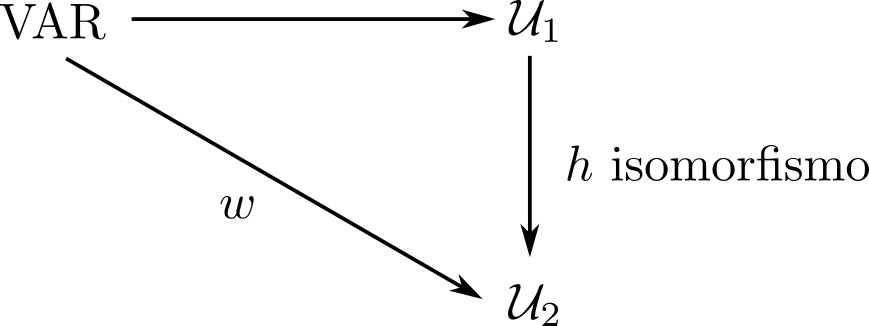
\includegraphics[width=0.58\textwidth]{corolario-aplicacion-iso-ida-1}
        \caption{Relación entre $\mathrm{VAR}$ y $\mathcal{U}_1$, 
        $\mathcal{U}_2$}
    \end{figure}
    ¿Cómo construimos una $v$ que satisfaga lo anterior? Aprovechando la
    biyectividad (en particular que es sobreyectiva):
    \begin{figure}[H]
        \centering
        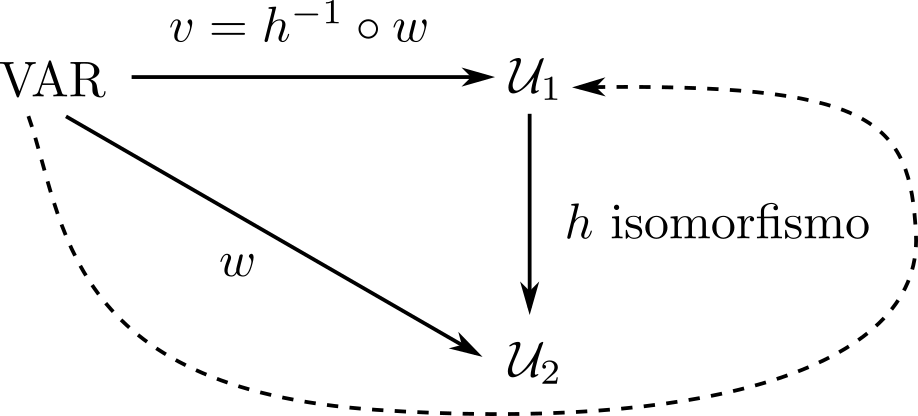
\includegraphics[width=0.58\textwidth]{corolario-aplicacion-iso-ida-2}
        \caption{Construcción de $v$.}
    \end{figure}
    Entonces $v$ es $v = h^{-1} \circ w$. Notemos que al aplicar $h$ 
    obtenemos $w$, que es precisamente lo que buscamos.

    Para la vuelta la idea es la misma: definimos $w = h \circ v$.
    \begin{figure}[H]
        \centering
        \includegraphics[width=0.58\textwidth]{%
            corolario-aplicacion-iso-vuelta}
        \caption{Construcción de $w$.}
    \end{figure}
    En ambos casos estamos usando el Teorema \ref{teo:equiv-isomorfs}:
    \begin{gather*}
        \mathcal{I}_1 \vDash \alpha[v] 
        \iff \mathcal{I}_2 \vDash \alpha [h \circ v] 
    \end{gather*}
\end{proof}

\subsubsection{Ejemplo}

$\mathcal{L}$ con $=$ y $f^2$. 
$\mathcal{I}_1 = (\mathbb{N}, +)$; $\mathcal{I}_2 = (\mathbb{N}, \, .)$

Probar que $\mathcal{I}_1 \not\approx \mathcal{I}_2$
\begin{gather*}
    \alpha = \exists \; x \quad \forall y \quad f^2 (x,y) = x
\end{gather*}

En $\mathcal{I}_1$:
\begin{align*}
    & \exists \; x \quad \forall y \quad x+y = x \\
    \iff & \exists \; x \quad \forall y \quad y = 0
\end{align*}

Falso. Basta tomar $y = 2$. $\implies V_{\mathcal{I}_1}(\alpha) = 0$

En $\mathcal{I}_2$:
\begin{align*}
    & \exists \; x \quad \forall y \quad x \, . \, y = x \\
    \iff & \exists \; x \quad \forall y \quad x(y-1) = 0
\end{align*}

Tomo $x = 0$ y es verdadero. $\implies V_{\mathcal{I}_2}(\alpha) = 1$

Luego
\begin{gather*}
    \underbrace{0 = V_{\mathcal{I}_1} (\alpha)}_{%
    \mathcal{I}_1 \text{ no es modelo de } \alpha}
    \neq 
    \underbrace{V_{\mathcal{I}_2} (\alpha) = 1}_{%
    \mathcal{I}_2 \text{ es modelo de } \alpha}
\end{gather*}

\begin{gather*}
    \therefore ~ \notamath{Por Corolario \ref{corol:no-equiv-isomorf} }
    \mathcal{I}_1 \not\approx \mathcal{I}_2
\end{gather*}

\medskip

\begin{corolario}{}{no-equiv-isomorf-2}
    Sea $\mathcal{L}$ de primer orden.

    Sea $\mathcal{I}$ interpretación de $\mathcal{L}$ 
    con universo $\mathcal{U}$.

    $F: \mathcal{U} \to \mathcal{U}$ isomorfismo.

    \medskip

    Entonces $u \in \mathcal{U}$ distinguible $\implies F(a) = a$
\end{corolario}

¿Para qué nos sirve? Para probar que un elemento no es distinguible.

\begin{proof} \phantom{.}

    $a$ es distinguible 
    \nota{$a, b \in \mathcal{U}$}%
    $\implies$ $\exists \; \alpha(x) / 
    \underbrace{\overbrace{V_{\mathcal{I},v_{x=a}} (\alpha)= 1}^{%
    \circled{1}}}_{%
        \mathcal{I} \vDash \alpha [v_{x=a}]}$ y 
    $\overbrace{V_{\mathcal{I},v_{x=b}} (\alpha)= 0}^{\circled{2}}$ 
    si $b \neq a$.

    Aplicando el Teorema \ref{teo:equiv-isomorfs}:
    \begin{gather*}
        \mathcal{I} \vDash \alpha [F \circ v_{x=a}] \iff
        \notamath{$v$ ``manda'' $x$ a $a$, y
        al aplicarle $F$ lo ``manda'' a F(a)}
        \mathcal{I} \vDash \alpha [(F \circ v)_{x= F(a)}]
    \end{gather*}

    Esto nos está diciendo que $\alpha$ es verdadera en $\mathcal{I}$ cuando
    la valuación $(F \circ v)$ manda $x$ a $F(a)$.

    Además, por \circled{1} y \circled{2}, sabemos que la fórmula es verdadera
    en $y$ cuando $x = a$ y falsa cuando va a cualquier elemento distinto 
    de $a$.

    \begin{gather*}
        \therefore ~ F(a) = a
    \end{gather*}

\end{proof}



\pagebreak



\subsubsection{Ejemplo}

Sea $\mathcal{L}$ con $=$ y $P^2$; $\mathcal{I} = (\mathcal{U}, \leq)$;
$\mathcal{U} = \{ a, b, c, d \}$.

\nota{$a \leq b$\\ $a \leq c$\\ $b \leq d$\\ $c \leq d$}%
\begin{figure}[H]
    \centering
    \includegraphics[width=0.40\textwidth]{%
    corolario-2-aplicacion-iso-ej-consigna}
    \caption{Relación de orden del universo.}
\end{figure}

Hallar los elementos distinguibles en $\mathcal{I}$.

\medskip

$a$ es distinguible porque
\begin{gather*}
    \alpha(x) = \forall y \quad P(x,y)\\
    V_{\mathcal{I}}(\alpha) = 1 \iff
    \forall y \quad x \leq y \implies \text{ en particular } x \leq a
    \implies x = a
\end{gather*}

Por otro lado $a \leq y ~ \forall y \implies V_{\mathcal{I}}(\alpha)=1$

Análogamente, $d$ es distinguible.
\begin{gather*}
    \beta(x) = \forall y \quad P(y,x)
\end{gather*}

\nota{$F$ es biyectiva.}%
Definimos $F: \mathcal{U} \to \mathcal{U} / F(a) = a; F(d) = d; F(b) = c
\text{ y }F(c) = b$.

Para ser un isomorfismo:
\begin{align*}
    x \leq y &\iff F(x) \leq F(y)\\
    a \leq b &\iff \underbrace{F(a)}_{a} \leq \underbrace{F(b)}_{c}\\
    a \leq a &\iff \underbrace{F(a)}_{a} \leq \underbrace{F(a)}_{a}\\
    a \leq d &\iff \underbrace{F(a)}_{a} \leq \underbrace{F(d)}_{d}\\
    \vdots
\end{align*}
En total son 9 renglones de desigualdades.

Una manera más corta es ayudándonos con los diagramas de Hasse.
\begin{figure}[H]
    \centering
    \includegraphics[width=0.45\textwidth]{%
    corolario-2-aplicacion-iso-ej-ans}
    \caption{Solución utilizando un diagrama de Hasse.}
\end{figure}

Como el diagrama es válido, se cumple $x \leq y \iff F(x) \leq F(y)$ y,
por lo tanto, $F$ es un isomorfismo.

En conclusión, como $F(b) \neq b$ $\implies b$ no es distinguible; y como
$F(c) \neq c$ $\implies c$ no es distinguible.


\bigskip
\textit{Noni:}
Notemos que con esto NO podemos probar que, como $F(a) = a$, entonces $a$ es
distinguible. El corolario es una implicación, no un sí y sólo sí.
Queda de tarea probar que la identidad siempre es un isomorfismo de $y$ en
$y$ con lo cual todos los elementos serían distinguibles, lo cual es falso
por lo que acabamos de demostrar.

Entonces para probar que los elementos son distinguibles, hay que encontrar
la fórmula que exprese el conjunto con dicho elemento. Para encontrar que
los elementos no son distinguibles, hay que encontrar un isomorfismo que
mueva dichos elementos.

\bigskip

\begin{corolario}{}{}
    Sea $\mathcal{L}$ un lenguaje de primer orden y sea $\mathcal{I}$ una
    interpretación de $\mathcal{L}$ con universo $\mathcal{U}$.

    Sea $F: \mathcal{U} \to \mathcal{U}$ un isomorfismo.

    \medskip

    Entonces
    \begin{gather*}
        \underbrace{F(A) \subseteq A}_{F(a) \, \in \, A ~ \forall a \in A}
        \quad \forall A \subseteq \mathcal{U}
    \end{gather*}
\end{corolario}

\begin{proof} \phantom{.}
    Tarea.

    Notemos que el corolario anterior es un caso particular de este.
\end{proof}

¿Para qué sirve? Para probar que un conjunto no es expresable.

\subsubsection{Ejemplo}

Sea $\mathcal{L}$ un lenguaje de 1\textsuperscript{er.} orden con $=$ y $f^2$.
Sea $\mathcal{I} = (\mathbb{Z}, +)$.

¿$A = \mathbb{N}$ es expresable?

\nota{Tarea: biyectiva}%
Defino $F: \mathbb{Z} \to \mathbb{Z} / F(x) = -x$
\begin{itemize}
    \item $F(x+y) = -(x+y) = -x + (-y) = F(x) + F(y)$
    \item $x = y \iff F(x) = F(y)$
\end{itemize}

Entonces $F$ es un isomorfismo.

Supongo $\mathbb{N}$ expresable $\implies F(\mathbb{N}) \subseteq \mathbb{N}$
pero $F(2) = -2 \notin \mathbb{N}$.
¡Absurdo!

\begin{center}
    $\therefore ~ A = \mathbb{N}$ no es expresable en $\mathcal{I}$.
\end{center}



\begin{corolario}{}{}
    Sea $\mathcal{L}$ un lenguaje de primer orden. 

    Sean $\mathcal{I}_1$ e $\mathcal{I}_2$ interpretaciones
     e $\mathcal{I}_1 \approx \mathcal{I}_2$.

    \medskip

    Si $a \in \mathcal{U}_1$ es distinguible en $\mathcal{I}_1$
    \begin{center}
        $\implies h(a) \in \mathcal{U}_2$ es distinguible en $\mathcal{I}_2$
    \end{center}
\end{corolario}

¿Para qué nos sirve? Para armar un isomorfismo.

\begin{proof} \phantom{.}

    Sabemos que: 
    \nota{Por el Teorema \ref{teo:equiv-isomorfs}}%
    $\mathcal{I}_1 \vDash \alpha[v] \overbrace{\iff}^{\bigstar}
    \mathcal{I}_2 \vDash \alpha[h \circ v]$.

    Si $a \in \mathcal{U}_1$ es distinguible
    \begin{align*}
        &\implies \exists \; \alpha(x) \text{ que expresa } \{ a \} \\
        &\implies \mathcal{I}_1 \vDash \alpha(x)[v_{x=a}] \text{ y }
        \mathcal{I}_1 \not\vDash \alpha(x)[v_{x=b}] \text{ con } b \neq a\\
        &\implies \mathcal{I}_2 \vDash \alpha(x)[%
        \underbrace{h \circ v_{x=a}}_{{(h \circ v)}_{x = h(a)}}%
        ] \text{ y }
        \mathcal{I}_2 \not\vDash \alpha(x)[%
        \underbrace{h \circ v_{x=b}}_{{(h \circ v)}_{x = h(b)}}%
        ] 
        \text{ con } \underbrace{b \neq a}_{h(b) \neq h(a)} 
        \notamath{Por $\bigstar$}
    \end{align*}

    \begin{center}
        $\therefore ~ \alpha(x)$ distingue $h(a)$ en $\mathcal{I}_2$.
    \end{center}
\end{proof}

%% Copyright (c) 2022 Martín E. Zahnd
%%
%% This code is licensed under MIT license (see LICENSE.txt for details)
%%
\chapter{Lenguaje S}
%\graphicspath{ {./teoria/resources/lenguaje-s/} }

\section{Variables, etiquetas e instrucciones}
\begin{definicion}{Variables}{}
    Existen tres tipos de variables, las cuales no se declaran:
   \begin{enumerate}
       \item \textbf{Variables de entrada:} $X_1, X_2, X_3, \dotsc$

       \item \textbf{Variables temporales:} $Z_1, Z_2, Z_3, \dotsc$

       \item \textbf{Variable de salida:} $Y$
   \end{enumerate} 

   El tipo de datos es $\mathbb{N}$ y las variables auxiliares y la de salida
   comienzan inicializadas en 0.
\end{definicion}

\begin{definicion}{Etiquetas}{}
    Las etiquetas se representan como:
    \begin{gather*}
        A_1, B_1, C_1, D_1, E_1, A_2, \dotsc
    \end{gather*}
\end{definicion}

\begin{definicion}{Instrucciones}{}
    Existen tres tipos de instrucciones:
    \begin{enumerate}
        \item Sea $V$ una variable.
            \begin{gather*}
                V \gets V + 1
            \end{gather*}

            Si la variable $V$ tiene el valor $n \in \mathbb{N}$, luego de
            ejecutarse la instrucción va a tener el valor $n+1$.
        \item Sea $V$ una variable.
            \begin{gather*}
                V \gets V - 1
            \end{gather*}
            Si la variable $V$ tiene el valor $n \in \mathbb{N}_{\geq 1}$, 
            luego de ejecutarse la instrucción va a tener el valor $n-1$.
            Si $V$ tiene el valor 0, luego de ejecutarse queda con el mismo
            valor.
        \item Sea $V$ una variable y $L$ una etiqueta.
            \begin{gather*}
                IF ~ V \neq 0 \quad GOTO ~ L
            \end{gather*}

            Si la variable $V$ tiene el valor 0, se pasa a la próxima 
            instrucción; si tiene un valor distinto de cero, se pasa a la 
            primer instrucción del programa a la cual la antecede la etiqueta
            $L$.
    \end{enumerate}

    A cada instrucción la puede anteceder una etiqueta, la cual se escribe
    entre corchetes:
    \begin{gather*}
        [L] \quad \text{Instrucción}
    \end{gather*}
\end{definicion}

\subsection{Programa}

\begin{definicion}{Programa}{}
   Un programa es una lista finita de instrucciones $I_1, I_2, \dotsc, I_n$
   que se escriben una debajo de la otra.
\end{definicion}

\subsubsection{Ejemplos}

\begin{itemize}
    \item Dado el siguiente programa:
        \begin{align*}
            [A_1] \quad &X_1 \gets X_1 - 1 \\
                        &Y \gets Y + 1 \\
                        &IF ~ X \neq 0 \quad GOTO ~ A_1
        \end{align*}

        Veamos qué ocurre si entramos con diferentes valores:
        
        \begin{center}
        \begin{tabular}{c c c}
            \begin{tabular}{c | c}
                $X$ & $Y$ \\
                \hline
                2 & 0 \\
                1 & 1 \\
                0 & 2 \\
            \end{tabular}

            &

            \begin{tabular}{c | c}
                $X$ & $Y$ \\
                \hline
                1 & 0 \\
                0 & 1 \\
                \phantom{0} & \phantom{0} \\
            \end{tabular}

            &

            \begin{tabular}{c | c}
                $X$ & $Y$ \\
                \hline
                0 & 0 \\
                0 & 1 \\
                \phantom{0} & \phantom{0} \\
            \end{tabular}
        \end{tabular}
        \end{center}

        Este programa implementa $f: \mathbb{N} \to \mathbb{N} / f(n) =
        \begin{cases}
            n & n \neq 0 \\
            1 & n = 0
        \end{cases}$

    \item Supongamos que el programa tiene una única instrucción:
        \begin{gather*}
            Y \gets Y - 1
        \end{gather*}
        
        Este programa computa la función $f: \mathbb{N} \to \mathbb{N}/f(n)=0$.

        Es decir, el programa presentado es una forma de implementar la 
        función constante cero.


        \bigskip
        \textit{Observación:}
        Notemos que
        \begin{align*}
            &X_1 \gets X_1 - 1 \\
            &Y \gets Y - 1
        \end{align*}
        es un programa que computa la misma función.

        Entonces dos programas distintos pueden computar la misma función.

    \item Dado el siguiente programa:
        \begin{gather*}
           \left.\begin{aligned}
                   Y &\gets Y + 1 \\
                Y &\gets Y + 1 \\
                  &\vdots \\
                Y &\gets Y + 1
               \end{aligned}\right\} k \text{ instrucciones}
        \end{gather*}

        Este programa computa la función $f: \mathbb{N} \to \mathbb{N}/f(n)=k$

    \item Dado el siguiente programa:
        \begin{gather*}
            [A_1] \quad IF ~ X_1 \neq 0 \quad GOTO ~ A_1
        \end{gather*}

        \begin{center}
        \begin{tabular}{c c}
            \begin{tabular}{c | c}
                $X_1$ & $Y$ \\
                \hline
                2 & 0 \\
                2 & 0 \\
                2 & 0 \\
                \vdots & 0 \\
            \end{tabular}

            &

            \begin{tabular}{c | c}
                $X_1$ & $Y$ \\
                \hline
                0 & 0 \\
            \end{tabular}
        \end{tabular}
        \end{center}

        Notemos que el programa nunca termina si entramos con una constante
        distinta de cero.

        Entonces este programa computa la función 
        \nota{$Dom(f) = \{ 0 \}$}%
        $f: \mathbb{N} \to \mathbb{N} /
        f(x) = \begin{cases}
            \uparrow & x \neq 0 \\
            0 & x = 0
        \end{cases}$

        Donde $\uparrow$ significa que no está definida la función, es decir,
        el programa nunca termina.

    \item \textbf{Función identidad}

        Dado el siguiente programa
        \begin{align*}
            [A] \quad &IF ~ X_1 \neq 0 \quad GOTO ~ B \\
                        &Z_1 \gets Z_1 + 1 \\
                        &IF ~ Z_1 \neq 0 \quad GOTO ~ E \\
            [B] \quad &X_1 \gets X_1 - 1 \\
                        &Y \gets Y + 1 \\
                        &Z_1 \gets Z_1 + 1 \\
                        &IF ~ Z_1 \neq 0 \quad GOTO ~ A
        \end{align*}

        Como la etiqueta $E_1$ no antecede a ninguna instrucción, cuando el
        programa busca dicha etiqueta termina.

        Este programa computa la función identidad:
        $f: \mathbb{N} \to \mathbb{N} / f(x) = x$
\end{itemize}


\section{Macros}

\begin{definicion}{Macro}{}
    Una macro es una pseudoinstrucción que representa un segmento de 
    un programa.
\end{definicion}

\medskip

\begin{definicion}{Expansión de una macro}{}
    Cada vez que en un programa $\mathcal{P}$ aparece una macro, la misma se 
    debe reemplazar por el segmento del programa que representa.
    Este proceso de denomina \textit{expansión de la macro}.
\end{definicion}

Debemos ser cuidadosos de que las variables auxiliares y las etiquetas que
se utilicen para expandir una macro no aparezcan en otras instrucciones del
programa.

\subsubsection{Ejemplos de macros}

\begin{itemize}
    \item La macro \textit{salto incondicional} se representa como:
        \begin{gather*}
            GOTO ~ L
        \end{gather*}
        siendo $L$ una etiqueta.

        Esta macro se expande de la siguiente manera:
        \begin{align*}
            &V \gets V + 1 \\
            &IF ~ V \neq 0 \quad GOTO ~ L
        \end{align*}

        Donde $V$ es una variable temporal que no aparece en el resto del 
        código.

    \item La macro \textit{asignación de cero} se representa como:
        \begin{gather*}
            V \gets 0
        \end{gather*}

        Y se expande como
        \begin{align*}
            [L] \quad &V \gets V - 1 \\
                      &IF ~ V \neq 0 \quad GOTO ~ L
        \end{align*}

        Donde $L$ es una etiqueta que no aparece en el resto del programa.

    \item La macro \textit{asignación de variable} se representa como
        \begin{gather*}
            V_1 \gets V_2
        \end{gather*}

        Y se expande:
        \nota{Recordar que las etiquetas que aparecen en esta macro
        \underline{no} deben ser utilizadas en el programa donde se utiliza la
        macro. Lo mismo para la variable auxiliar.}%
        \begin{align*}
                        &V_1 \gets 0 \\
            [L_1] \quad &IF ~ V_2 \neq 0 \quad GOTO ~ L_2 \\
                        &GOTO ~ L_3 \\
            [L_2] \quad &V_2 \gets V_2 -1 \\
                        &V_1 \gets V_1 + 1 \\
                        &Z_1 \gets Z_1 + 1 \\
                        &GOTO ~ L_1 \\
            [L_3] \quad &IF ~ Z_1 \neq 0 \quad GOTO ~ L_4 \\
                        &GOTO ~ L_5 \\
            [L_4] \quad &Z_1 \gets Z_1 - 1 \\
                        &V_2 \gets V_2 + 1 \\
                        &GOTO ~ L_3
        \end{align*}

        \bigskip
        \textit{Observación:}
        Notemos que si cambiamos $V_1$ por $Y$ y $V_2$ por $X_1$ y vemos la
        macro como un programa completo este computaría la función identidad.
        A diferencia del ejemplo en la sección anterior, este programa 
        resguardaría el valor de entrada.
\end{itemize}

\subsubsection{Ejemplos de programas con macros}

\begin{itemize}
    \item \textbf{Función suma} \label{ej:funcion-suma}

        El siguiente programa computa la función 
        $f: \mathbb{N} \times \mathbb{N} \to \mathbb{N}/f(x_1, x_2) = x_1+x_2$

        \begin{align*}
                        &Y \gets X_1 \\
                        &Z_1 \gets X_2 \\
            [B_1] \quad &IF ~ Z_1 \neq 0 \quad GOTO ~ A_1 \\
                        &GOTO ~ E_1 \\
            [A_1] \quad &Z_1 \gets Z_1 - 1 \\
                        &Y \gets Y + 1 \\
                        &GOTO ~ B_1
        \end{align*}

        A partir de ahora podemos usar el macro
        \begin{gather*}
            V_1 \gets V_2 + V_3
        \end{gather*}

    \item \textbf{Función producto} \label{ej:funcion-producto}

        El siguiente programa computa la función 
        $f: \mathbb{N} \times \mathbb{N} \to \mathbb{N}/f(x_1, x_2) = x_1 x_2$

        \begin{align*}
                        &Z_2 \gets X_2 \\
            [B_1] \quad &IF ~ Z_2 \neq 0 \quad GOTO ~ A_1 \\
                        &GOTO ~ E_1 \\
            [A_1] \quad &Z_2 \gets Z_2 - 1 \\
                        &Z_1 \gets X_1 + Y \\
                        &Y \gets Z_1 \\
                        &GOTO ~ B_1
        \end{align*}

    \item \textbf{Función sucesor} \label{ej:funcion-sucesor}

        El siguiente programa computa la función
        $suc \mathbb{N} \to \mathbb{N} / suc(x) = x + 1$

        \begin{align*}
            &Y \gets X_1 \\
            &Y \gets Y + 1
        \end{align*}

    \item \textbf{Función proyección} \label{ej:funcion-proyeccion}

        \nota{$1 \leq i \leq k$}%
        $\Pi^k_i: {\mathbb{N}}^k \to \mathbb{N} / 
        \Pi_i (x_1, \dotsc, x_i, \dotsc, x_k) = x_i$

        Basta con cambiarle al programa que computa la función identidad su 
        variable $X_1$ por la variable $X_i$, 
        donde $X_i$ es la i-ésima variable que se quiere proyectar.
        \begin{align*}
            &Y \gets X_i
        \end{align*}
\end{itemize}

\bigskip
\textit{Observación:}
Si podemos programar la función $f: \mathbb{N}^k \to \mathbb{N}$, entonces
podemos implementar el macro
\begin{gather*}
    Z \gets f(V_1, \dotsc, V_k)
\end{gather*}

Si $\mathcal{P}$ es el programa  de $f$, cambio las apariciones de $Y$ por la
variable $Z$ y después las apariciones de $X_1, \dotsc, X_k$ por 
$V_1, \dotsc, V_k$, respectivamente, y el macro se expande como
\begin{gather*}
   \begin{aligned}
        Z_1 &\gets V_1 \\
        Z_2 &\gets V_2 \\
          &\vdots \\
        Z_k &\gets V_k \\
        \mathcal{P} \\
        V_n &\gets Z_1 \\
          &\vdots \\
        V_k &\gets Z_k \\
    \end{aligned}
    \notamath{$Z_1, \dotsc, Z_k$ no aparecen en $\mathcal{P}$ ni en el resto 
    del programa}
\end{gather*}

\section{Descripciones de programas}

\subsection{Estado de un programa}

\begin{definicion}{Estado de un programa}{}
    El estado de un programa $\mathcal{P}$ es una lista finita de ecuaciones 
    de la forma
    \begin{gather*}
        V = m
    \end{gather*}

    Donde $V$ es una variable y $m \in \mathbb{N}$.

    \medskip

    Hay una única ecuación para cada variable que aparece en $\mathcal{P}$.
\end{definicion}

\subsubsection{Ejemplo}

Dado el siguiente programa $\mathcal{P}$:
\begin{align*}
    [A_1] \quad &X_1 \gets X_1 - 1 \\
                &Y \gets Y + 1 \\
                &IF ~ X_1 \neq 0 \quad GOTO ~ A_1
\end{align*}

Entonces los estados de $\mathcal{P}$ son:
\begin{align*}
    X_1 &= 2, Y = 1 \\
    X_1 &= 3, Y = 1, Z_1 = 0 \\
    X_1 &= 5, Y = 1, Z_1 = 6
\end{align*}

Notemos que no es necesario que los estados sean alcanzados.

\medskip

Por otra parte, las siguientes secuencias \underline{no} son estados:
\begin{align*}
    X_1 = 2 \quad \text{Falta una ecuación asociada a la variable } Y \\
    X_1 = 2, Z_1 = 3 \quad \text{Falta una ecuación asociada a la 
    variable } Y \\
    Y = 1, X_1 = 6, Y = 2 \quad \text{Hay dos secuencias asociadas a la 
    variable } Y
\end{align*}

\subsection{Descripción instantánea de un programa o Snapshot}

\begin{definicion}{Descripción instantánea de un programa}{}
    Supongamos que un programa $\mathcal{P}$   tiene longitud $n$, es decir,
    consta de $n$ instrucciones $I_1, I_2, \dotsc, I_n$.

    \begin{itemize}
        \item Para un estado $\sigma$ de $\mathcal{P}$ y un 
            $i \in \{ 1,2,\dotsc,n+1\}$ tenemos que el par $(i, \sigma)$ es 
            una descripción instantánea de $\mathcal{P}$, la cual se llama 
            terminal si $i = n+1$.

            $i$ nos dice a qué instrucción apunta antes de ser ejecutada, y
            en $\sigma$ están los valores de las variables antes de ejecutar
            la instrucción $i$.

        \item Para una $(i, \sigma)$ no terminal se puede definir su sucesor 
        $(j, \tau)$:
        \begin{enumerate}
            \item La i-ésima instrucción de $\mathcal{P}$ es $V \gets V+1$.

            Entonces $j = i + 1$, y $\tau = \sigma$ salvo que la ecuación 
            $V=m$ en $\sigma$ va a ser $V=m+1$ en $\tau$

            \item La i-ésima instrucción de $\mathcal{P}$ es $V\gets V-1$.

                Entonces $j= i + 1$, y $\tau = \sigma$ salvo que
                $V=m$ en $\sigma$ será 

                $V = \begin{cases}
                    m - 1 & \text{si } m > 0 \\
                    0 & \text{si } m = 0
                \end{cases} ~$ en $\tau$.
                
            \item La i-ésima instrucción de $\mathcal{P}$ es 
                $IF ~ V \neq 0 \quad GOTO ~ L$

                Entonces 
                $\tau = \sigma$ y 
                \begin{itemize}
                    \item Si $V=0$ en $\sigma$
                        $\implies$
                        $j=i+1$
                    \item Si $V \neq 0$ en $\sigma$
                        $\implies$

                        $j = \begin{cases} 
                    \min{\{ k: I_k \text{ tiene etiqueta } L \}} & \text{si 
                    existe } [L] ~ I_k \\
                    n+1 & \text{si no existe } [L] ~ I_k
                \end{cases}$
                \end{itemize}
        \end{enumerate}
    \end{itemize}
\end{definicion}

\subsection{Cómputo}
\begin{definicion}{Cómputo}{}
    Un cómputo de un programa $\mathcal{P}$ a partir de una descripción 
    instantánea $d_1 = (i, \sigma)$ es una lista 
    $d_1, d_2, \dotsc, d_k$ de descripciones
    instantáneas de $\mathcal{P}$ tales que $d_{j+1}$ es el sucesor de $d_j$.

    Siendo $ 1 \leq j \leq k-1$, y $d_k$ la descripción 
    instantánea terminal.
\end{definicion}

\subsubsection{Ejemplo}

Para el siguiente programa $\mathcal{P}$:
\begin{align*}
    [A_1] \quad &X_1 \gets X_1 - 1 \\
                &Y \gets Y + 1 \\
                &IF ~ X_1 \neq 0 \quad GOTO ~ A_1
\end{align*}

El cómputo a partir de $d_1 = \{ 1, X_1 = 2, Y = 0 \}$ es:
\begin{align*}
    d_2 &= \{ 2, X_1 = 1, Y = 0 \} \\
    d_3 &= \{ 3, X_1 = 1, Y = 1 \} \\
    d_4 &= \{ 1, X_1 = 1, Y = 1 \} \\
    d_5 &= \{ 2, X_1 = 0, Y = 1 \} \\
    d_6 &= \{ 3, X_1 = 0, Y = 2 \} \\
    d_7 &= \{ 4, X_1 = 0, Y = 2 \}
\end{align*}

\subsection{Estado inicial}
\begin{definicion}{Estado inicial}{}
    Sea $\mathcal{P}$  un programa y sean $u_1, \dotsc, u_m$ números naturales.
    
    \medskip

    El estado inical de $\mathcal{P}$ para $u_1, \dotsc, u_m$ es el estado
    $\sigma_1$  definido como
    \begin{gather*}
        \notamath{$j>m$}
        \sigma_1 = (X_1 = u_1, X_2 = u_2, \dotsc, X_m = u_m, X_j = 0, Z_j = 0,
        Y = 0)
    \end{gather*}
    \nota{En cuyo caso no se escriben}%
    Donde $X_j$ y $Z_j$ pueden no aparecer en el programa.

    Por lo tanto la descripción inicial de $\mathcal{P}$ para $u_1,\dotsc,u_m$
    es $d_1 = (1, \sigma_1)$.
\end{definicion}

\medskip

\begin{definicion}{Cómputo a partir del estado inicial}{}
    Sea $\mathcal{P}$ un programa, sean $u_1, \dotsc, u_m$ números naturales
    y $\sigma_1$ el estado inicial para ellos.

    \medskip

    Entonces existen dos posibilidades:
    \begin{enumerate}
        \item Hay un cómputo de $\mathcal{P}$: $d_1, \dotsc, d_k$, siendo
            $d_1 = (1, \sigma_1)$.

            \bigskip
            \textbf{Notación:}
            $\Psi_{\mathcal{P}}^{m} (u_1, \dotsc, u_k)$ es el valor de $Y$
            en la descripción instantánea $d_k$.

        \item Existe una secuencia infinita $d_1, d_2, \dotsc$ siendo
            \nota{No hay tal cómputo}%
            $d_1 = (1, \sigma_1)$ y $d_{i+1}$ el sucesor de $d_i$.

            \bigskip
            \textbf{Notación:}
            $\Psi_{\mathcal{P}}^{m} (u_1, \dotsc, u_k) = \uparrow$ significa
            que $\Psi_{\mathcal{P}}^{m} (u_1, \dotsc, u_k)$ está indefinido.
    \end{enumerate}
\end{definicion}

\subsection{Función computable}

\begin{definicion}{Función parcialmente computable}{}
    Una función $f$ es parcialmente computable si existe un programa 
    $\mathcal{P}$ tal que $f = \Psi_{\mathcal{P}}^m$

    \medskip

    Donde si $x = (x_1, \dotsc, x_k) \in \mathbb{N}^k$ entonces
    \begin{itemize}
        \item Si $x \in Dom(f) \implies$
            \nota{Para todo \\$(x_1, \dotsc, x_m) \in \mathbb{N}^k$}%
            $f(x_1, \dotsc, x_k) = \Psi_{\mathcal{P}}^m (x_1, \dotsc, x_k)$
    \item Si $x \notin Dom(f) \implies$
            $\Psi_{\mathcal{P}}^m (x_1, \dotsc, x_k) = \uparrow$
    \end{itemize}
\end{definicion}

\medskip

\begin{definicion}{Función total}{}
    Sea $f$ una función.

    \medskip

    Decimos que $f$ es total si su dominio es $\mathbb{N}^m$.
\end{definicion}

\medskip

\nota{Noni la llama \\``computable'' a secas;
    Santiago usa el nombre completo: ``total computable''.}
\begin{definicion}{Función total computable}{}
    Una función $f: \mathbb{N}^k \to \mathbb{N}$ es total computable si es 
    parcialmente computable y total.
\end{definicion}

\bigskip
\textit{Observación:}
Notemos que el mismo programa puede servir para computar funciones de
$1, 2, 3, \dotsc$ variables.

Por lo tanto si en $\mathcal{P}$ aparece $X_n$ y no aparece $X_i$, con $i>n$,
hay dos opciones:
\begin{enumerate}
    \item Si sólo se especifican $m < n$ valores de entrada, entonces 
        $X_{m+1}, \dotsc, X_n$ toman el valor 0.
    \item Si se especifican $m>n$ valores de entrada, $\mathcal{P}$ ignorará
        $u_{n+1}, \dotsc, u_m$.
\end{enumerate}

\subsubsection{Ejemplo}

Sea el programa $\mathcal{P}$
\begin{gather*}
    [A_1] \quad IF ~ X_1 \neq 0 \quad GOTO ~ A_1
\end{gather*}

Notemos que $\Psi_{\mathcal{P}}^{1} (x) = \begin{cases}
    0 & x = 0\\
    \uparrow & x \neq 0
\end{cases} ~$ pues:

\begin{align*}
    d_1 &= (1, X_1 = 0, Y = 0) \\
    d_2 &= (2, X_1 = 0, Y = 0) \notamath{Terminal}\\
    \\
    d_1 &= (1, X_1 = n, Y = 0) \notamath{$n>0$} \\
    d_2 &= (1, X_1 = n, Y = 0)\\
        & \implies d_j = d_1 ~ \forall j \in \mathbb{N}
\end{align*}
\begin{gather*}
    \therefore ~ \nexists \text{ un cómputo de } d_1 \text{ de } \mathcal{P}
\end{gather*}

La función $f$ que computa es parcialmente computable pues su dominio es 
$\{0\}$, siendo $f: \{ 0 \} \to \mathbb{N} / f(0) = 0$.

\bigskip


\section{Teorema}

\begin{teorema}{Composición de funciones computables}{composicion-computables}
    Sea $f: \mathbb{N}^k \to \mathbb{N}$ (parcialmente) computable.

    Sean $g_1, g_2, \dotsc, g_k: \mathbb{N}^m \to \mathbb{N}$ (parcialmente) 
    computables.

    \medskip

    Entonces $h: \mathbb{N}^m \to \mathbb{N}$ tal que
    \begin{gather*}
        \notamath{Es decir: \\
        $h = f \circ (g_1 \times g_2 \times \dotsc \times g_k)$}%
        h(x_1, \dotsc, x_m) = f(g_1 (x_1, \dotsc, x_m), g_2 (x_1, \dotsc, x_m),
    \dotsc, g_k (x_1, \dotsc, x_m))
    \end{gather*}

    \smallskip

    es (parcialmente) computable.
\end{teorema}

\begin{proof} \phantom{.}

    Como $f$ es (parcialmente) computable 
    $\implies \exists \; \mathcal{P}_f$ que
    la computa $\implies$ podemos armar una macro.

    Como $g_j$ es (parcialmente) computable 
    $\implies \exists \; \mathcal{P}_{g_j}$ 
    que la computa $\implies$ podemos armar una macro.

    Armo el siguiente programa para probar que $h$ es (parcialmente) 
    computable.

    \begin{align*}
        Z_1 \gets& g_1 (x_1, \dotsc, x_m) \\
        Z_2 \gets& g_w (x_1, \dotsc, x_m) \\
        \vdots & \\
        Z_k \gets& g_k (x_1, \dotsc, x_m) \\
        Y \gets& f(z_1, \dotsc, z_k)
    \end{align*}
\end{proof}

\medskip

\noindent\rule{\textwidth}{0.25pt}

\medskip

\textbf{Bonus:} libro recomendado por María Laura Noni.

``\textit{Introduction to Automata Theory, Languages, and Computation by 
Hopcroft, J. and Ullman, J}.''


%% Copyright (c) 2022 Martín E. Zahnd
%%
%% This code is licensed under MIT license (see LICENSE.txt for details)
%%
\chapter{Funciones RP}
% \graphicspath{ {./teoria/resources/funciones-rp/} }

\section{Esquemas recursivos}

\begin{definicion}{Esquema de recursión primitiva tipo I}{}
    Sea $h: \mathbb{N} \to \mathbb{N}$
    
    Sea $g: \mathbb{N}^2 \to \mathbb{N}$

    \medskip

    Decimos que $h$ se obtiene a partir de $g$ por un ERI si se puede escribir
    de la siguiente forma:
    \begin{align*}
        h(0) &= k \in \mathbb{N} \\
        h(n+1) &= g(n, h(n))
    \end{align*}
\end{definicion}

\medskip

\begin{teorema}{}{}
    \nota{ERI: ``Esquema Recursivo Primitivo tipo 1''}%
    Si $h$ se obtiene a partir de $g$ por un ERI y $g$ es computable, 
    entonces $h$ es computable.
\end{teorema}

\begin{proof} \phantom{.}
    \begin{align*}
        &Y \gets K \\
        [A_1] \quad &IF ~ X_1 = 0 \quad GOTO ~ E_1 
        \notamath{Def. en ej. de la práctica}\\
        &Y \gets g(Z_1, Y) \\
        &Z_1 \gets Z_1 + 1 \\
        &X_1 \gets X_1 - 1 \\
        &GOTO ~ A_1
    \end{align*}

    Notemos que
    \begin{center}
        \begin{tabular}{c | c | l}
            $X_1$ & $Z_1$ & $Y$ \\
            \hline
            $2$ & $0$ & $0$ \\
            $2$ & $0$ & $k = h(0)$ \\
            $1$ & $1$ & $g(0,k) = h(1)$ \\
            $0$ & $2$ & $g(1, g(0,k))=h(2)$
        \end{tabular}
    \end{center}
\end{proof}

\subsubsection{Ejemplo}
Demostrar mediante un ER que $f: \mathbb{N} \to \mathbb{N}/f(n) = n!$ es
computable.
\nota{$\mathrm{PROD(x,y)}$: Producto de $x$ e $y$ \\
$\mathrm{SUC}(x)$: Sucesor de $x$\\
$\Pi_j$: Proyección de la variable j-ésima}%
\begin{align*}
    f(0) &= 1 \\
    f(n+1) &= (n+1)! = (n+1) n! = (n+1) f(n) \underbrace{=}_{\text{Quiero}} 
    g(n, f(n))
\end{align*}

Defino $g: \mathbb{N}^2 \to \mathbb{N} / g(x,y) = 
\mathrm{PROD}(\mathrm{SUC}(x),y)$

\begin{align*}
    g(x,y) = \mathrm{PROD}(\mathrm{SUC}(\Pi_1 (x,y)), \Pi_2 (x,y)) \\
    g = \mathrm{PROD} \circ (\mathrm{SUC} \circ \Pi_1 \times \Pi_2)
\end{align*}

\smallskip

$g$ es computable por ser composición de funciones computables 
\nota{Ver los ejemplos en la \fullrefpage{ej:funcion-suma}{página}}%
(ya vimos que $\mathrm{PROD}$, $\mathrm{SUC}$ y $\Pi_j$ es computable).

\begin{center}
    $\therefore ~ f$ es computable por ser ERI a partir de $g$ computable.
\end{center} 

\bigskip

\nota{ERII}%
\begin{definicion}{Esquema de recursión primitiva tipo II}{}
    Sea $h: \mathbb{N}^{n+1} \to \mathbb{N}$
    
    Sea $g: \mathbb{N}^{n+2} \to \mathbb{N}$

    Sea $q: \mathbb{N}^{n} \to \mathbb{N}$

    \medskip

    Decimos que $h$ se obtiene por ERII a partir de $g$ y $q$ si puede 
    escribirse:
    \begin{align*}
        h(x_1, x_2, \dotsc, x_n, 0) &= q(x_1, \dotsc, x_n) \\
        h(x_1, x_2, \dotsc, x_n, y+1) &= g(x_1, \dotsc, x_n, y, 
        h(x_1,\dotsc, x_n, y))
    \end{align*}
\end{definicion}

\medskip

\begin{teorema}{}{}
    Sea $g: \mathbb{N}^{n+2} \to \mathbb{N}$

    Sea $q: \mathbb{N}^{n} \to \mathbb{N}$

    Sea $h: \mathbb{N}^{n+1} \to \mathbb{N}$ tal que se obtiene por ERII a 
    partir de $q$ y $g$.

    \medskip

    Si $q$ y $g$ son computables $\implies$ $h$ es computable.
\end{teorema}

\begin{proof} \phantom{.}
    \begin{align*}
        &Y \gets q(X_1, \dotsc, X_n) \\
        [A_1] \quad &IF ~ X_{n+1} = 0 \quad GOTO ~ E_1 \\
        &Y \gets g(x_1, \dotsc, x_n, Z_1, Y) \\
        &Z_1 \gets Z_1 + 1 \\
        &X_{n+1} \gets X_{n+1} - 1 \\
        &GOTO ~ A_1
    \end{align*}
\end{proof}

\section{Funciones iniciales} \label{sec:funciones-iniciales}

Las siguientes funciones se denominan \underline{funciones iniciales}.

\begin{definicion}{Función cero}{}
    \begin{gather*}
        \mathrm{CERO}: \mathbb{N} \to \mathbb{N} / \mathrm{CERO}(x) = 0
    \end{gather*}
\end{definicion}

\medskip

\begin{definicion}{Función sucesor}{}
    \begin{gather*}
        \mathrm{SUC}: \mathbb{N} \to \mathbb{N} / \mathrm{SUC}(x) = x+1
    \end{gather*}
\end{definicion}

\medskip

\begin{definicion}{Función proyección}{}
    \begin{gather*}
        \Pi_{j}^{n}: \mathbb{N}^{n} \to \mathbb{N} / 
        \Pi_{j}^{n}(x_1, \dotsc, x_n) = x_j
        \notamath{$1 \leq j \leq n$}
    \end{gather*}
\end{definicion}

\bigskip
\textit{Observación:}
$id: \mathbb{N} \to \mathbb{N} = \Pi_1^1: \mathbb{N} \to \mathbb{N}$

\bigskip
\textit{Observación:}
Las funciones iniciales son computables.

\begin{proof}
    \nota{En los ejemplos de programas en la sección del lenguaje S.
    \fullrefpage{ej:funcion-suma}{Página}}%
    Ya la hicimos.
\end{proof}

\section{Recursividad primitiva}

\nota{RP}%
\begin{definicion}{Recursividad primitiva}{rp}
    Una función es RP si es inicial o se obtiene aplicando finitas 
    ``operaciones válidas'' a las \nameref{sec:funciones-iniciales},
    siendo las operaciones válidas: composición, ERI y ERII.
\end{definicion}


\subsubsection{Ejemplos}

\begin{itemize}
    \item Probar que $\mathrm{SUMA}$ es RP, siendo
    \begin{gather*}
        \mathrm{SUMA}: \mathbb{N}^2 \to \mathbb{N} / \mathrm{SUMA}(x,y) = x+y
    \end{gather*}
    
    \begin{proof} \phantom{.}
    
        \begin{align*}
            \mathrm{SUMA}(x,0) &= x \underbrace{=}_{\text{Quiero}} g(x) \\
            \mathrm{SUMA} (x,y+1) &= x + (y+1) = (x+y) + 1 \\ 
            &= \mathrm{SUMA}(x,y)+1 \\
            &= \mathrm{SUC}(\mathrm{SUMA}(x,y))
            \underbrace{=}_{\text{Quiero}} 
            f(x,y,\mathrm{SUC}(\mathrm{SUMA}(x,y)))
        \end{align*}
    
        Definimos:
        \begin{itemize}
            \item $g: \mathbb{N} \to \mathbb{N} / g(x) = \Pi_1 (x)$
        \nota{$g=\Pi_1$ es inicial}%
    
            \item $f: \mathbb{N}^3 \to \mathbb{N} / 
                f(x,y,z) = z+1 = \mathrm{SUC}(\Pi_3 (x,y,z))$
    
            Es decir, 
            $f = \mathrm{SUC} \circ \Pi_3$ 
            es composición de iniciales.
        \end{itemize}
    
        Con lo cual me queda que $\mathrm{SUMA}$ es RP pues es un ERII de $g$
        inicial y de $f$ composición de iniciales.
    
    \end{proof}
    
    \textbf{Cuidado:} lo siguiente está mal.
    \begin{align*}
        \mathrm{SUMA}(x,2) &= \mathrm{SUC}( \mathrm{SUC} (x)) \\
        \mathrm{SUMA}(x,3) &= \mathrm{SUC}( \mathrm{SUC}( \mathrm{SUC} (x))) \\
        \implies \mathrm{SUMA}(x,y) &= \underbrace{\mathrm{SUC} \circ \dotsc 
        \circ \mathrm{SUC}}_{y \text{ veces}}(x) \\
        \implies \mathrm{SUMA} &= \mathrm{SUC} \circ \dotsc \circ \mathrm{SUC} 
        \circ \Pi_1
    \end{align*}
    
    El error es que no podemos decir cuántas veces estamos haciendo la 
    composición porque depende de dónde evaluamos $\mathrm{SUM}$, y no puede 
    depender de dónde la estamos evaluando.

    \item Probar que $\mathrm{PROD}$ es RP, siendo
    \begin{gather*}
        \mathrm{PROD}: \mathbb{N} \times \mathbb{N} \to \mathbb{N} /
        \mathrm{PROD}(x, y) = xy
    \end{gather*}

    Definamos
    \begin{gather*}
        \begin{cases}
            \mathrm{PROD}(x,0) = 0 = \mathrm{CERO}(x) & \\
            \mathrm{PROD}(x,y+1) = x(y+1) = xy+x = \mathrm{PROD}(x,y)+x &
        \end{cases}
    \end{gather*}

    Como queremos que 
    $\mathrm{PROD}(x,y)+x = g(x,y, \mathrm{PROD}(x,y))$,
    definimos $g: \mathbb{N}^3 \to \mathbb{N}$ tal que:
    \begin{gather*}
        g(x,y,z) = \mathrm{SUMA}(z,x) 
        = \mathrm{SUMA}(\Pi^3_3(x,y,z), \Pi^3_1(x,y,z))
    \end{gather*}

    Entonces, $\mathrm{PROD}$ es RP pues se obtiene a partir de funciones
    iniciales y finitos pasos de composición y ER.
\end{itemize}

\bigskip

\begin{teorema}{}{}
    Si $f: \mathbb{N}^k \to \mathbb{N}$ es RP $\implies$ $f$ es computable.
\end{teorema}

\begin{proof} \phantom{.}

    \begin{enumerate}
        \item Las funciones iniciales son computables (ya lo vimos).
        \item Composición de computables es computable (ya lo vimos).
        \item ERI y ERII de computables es computable (ya lo vimos).
    \end{enumerate}

    Como una función $f$ RP se obtiene aplicando finitas composiciones, ERI
    y ERII a iniciales que son funciones computables, entonces $f$ es 
    computable.

\end{proof}

\bigskip
\textit{Observación:}
Si $f$ no es total $\implies$ no es RP.

\bigskip
\textit{Observación:}
Existen funciones computables que no son RP.

\begin{proof}
    No la vemos.
\end{proof}

\subsubsection{Ejemplo}

\nota{\textit{Noni}: En alguna materia de programación la implementaron, así
que ya saben que es computable.}%
\textbf{Función de Ackermann}: Sea $A: \mathbb{N}^2 \to \mathbb{N}$ tal que
\begin{align*}
     &A(0,y) = y+1 \\
     &A(x+1,0) = A(x,1) \\
     &A(x+1,y+1) = A(x, A(x+1,y))
\end{align*}

Faltaría ver que la función no es RP.

\bigskip

\begin{teorema}{}{}
   \begin{enumerate}
       \item $f$ es composición de funciones RP $\implies$ $f$ es RP.
       \item $f$ se obtiene a partir de un ERI o un ERII de funciones RP
           $\implies$ $f$ es RP.
   \end{enumerate} 
\end{teorema}

\begin{proof} \phantom{.}

    \begin{enumerate}
        \item Defino $f: \mathbb{N}^k \to \mathbb{N} / 
        f = h \circ (g_1 \times \dotsc \times g_k)$

        Donde 
        $g_1, \dotsc, g_n: \mathbb{N}^k \to \mathbb{N}$ RP y 
        $h: \mathbb{N}^n \to \mathbb{N}$ RP.

        \begin{itemize}
        \item Como $g_j$ es RP, se obtuvo aplicando $m_j$ operaciones 
            \nota{``\hyperref[def:rp]{Operaciones permitidas}'': 
                Composiciones, ERI y ERII.\\
        $1 \leq j \leq n$}%
        permitidas a funciones iniciales.

        \item Como $h$ es RP, se obtuvo aplicando $m$ operaciones permitidas a
            funciones iniciales.
            
        \end{itemize}

        $\implies f$ se obtiene aplicando $1+m+m_1+\dots + m_n \in \mathbb{N}$
        operaciones a funciones iniciales.
        \begin{center}
            $\implies f$ es RP
        \end{center}

    \item 
        \begin{enumerate}[%
                        labelindent=*,
                        style=multiline,
                        leftmargin=*,
                        align=left,
                        leftmargin=2\parindent,
                        label=Caso \arabic*)]
            \item Tenemos
                $f: \mathbb{N} \to \mathbb{N}/ f(0) = k, f(n+1)=h(n,f(n))$,
                siendo $h: \mathbb{N}^2 \to \mathbb{N}$ RP.

                Como $h$ es RP, se obtuvo aplicando $k$ operaciones permitidas
                a funciones iniciales.

                $\implies f$ se obtiene aplicando $1+k$ operaciones permitidas
                a funciones iniciales.
                \begin{center}
                    $\implies f$ es RP
                \end{center}
            \item Tenemos $f: \mathbb{N}^{k+1} \to \mathbb{N} / \substack{%
                    f(x_1, \dotsc, x_k, 0) = g(x_1, \dotsc, x_k)\\
                    f(x_1, \dotsc, x_k, y+1) = h(x_1, \dotsc, x_k,y, 
                    f(x_1, \dotsc, x_k, y))}$

                Siendo $g: \mathbb{N}^k \to \mathbb{N}$ RP y 
                $h: \mathbb{N}^{k+2} \to \mathbb{N}$ RP.

                \begin{itemize}
                \item Como $g$ es RP, se obtuvo aplicando $m_g$ operaciones 
                permitidas a funciones iniciales.

                \item Como $h$ es RP, se obtuvo aplicando $m_h$ operaciones 
                permitidas a funciones iniciales.
                    
                \end{itemize}

                $\implies f$ se obtiene aplicando $m_g+m_h+1 \in \mathbb{N}$
                operaciones a funciones iniciales.
                \begin{center}
                    $\implies f$ es RP
                \end{center}
        \end{enumerate}
    \end{enumerate}
\end{proof}

\section{Predicados RP}

\begin{definicion}{Predicado}{}
    Un \textit{predicado} $P^k$ de $k$ variables es una relación $k$-aria de
    números naturales, es decir, $P^k \subseteq \mathbb{N}^k$.
\end{definicion}

\medskip

\begin{definicion}{Función característica}{}
    Se asocia a $P^k$ una función $C_{P^k}$, denominada
    \textit{función característica}, y definida como:
    \begin{gather*}
        C_{P^k} : \mathbb{N}^k \to \{ 0,1 \} /
        \notamath{$\overrightarrow{x} = (x_1, \dotsc, x_n)$, con 
                    $n \in \mathbb{N}$}
        C_{P^k} (\overrightarrow{x}) = \begin{cases}
            1 & \text{si } \overrightarrow{x} \in P^k\\
            0 & \text{si } \overrightarrow{x} \notin P^k
        \end{cases}
    \end{gather*}

    \bigskip
    \textbf{Notación:}
    $C_{P^k} = \Chi_{P^k}$
\end{definicion}

\medskip

\begin{definicion}{Predicado computable y RP}{}
    \begin{itemize}
        \item Decimos que ``$P^k$ es computable'' si 
            $C_{P^k}$ es computable.
        \item Decimos que ``$P^k$ es RP'' si 
            $C_{P^k}$ es RP.
    \end{itemize}

\end{definicion}

\subsubsection{Ejemplo}

Dada $P = \{ (x,y) \in \mathbb{N}^2 / x \leq y \} \subsetneq \mathbb{N}^2$.
Probar que $P$ es RP.

Definimos

\begin{gather*}
    C_{P}: \mathbb{N}^2 \to \mathbb{N} / C_{P} (x,y) =
    \begin{cases}
        1 & \text{si } x \leq y \\
        0 & \text{si } x > y
    \end{cases} =
    \begin{cases}
        1 & \text{si } x \restatruncada y  = 0\\
        0 & \text{si } x \restatruncada y \neq 0
    \end{cases} = \alpha(x \restatruncada y)
\end{gather*}

\nota{$\restatruncada$ significa ``resta truncada''.\\
$\alpha$ es una función de la práctica.\\
Ver ecuaciones \ref{eq:anexo-restatruncada} y \ref{eq:anexo-alpha}}%
Entonces $C_{P} 
= \alpha \circ \restatruncada \circ (\Pi_1 \times \Pi_2)$.

Por lo tanto, $C_{P}$ es composición de $\alpha$, $\restatruncada$,
$\Pi_j$, que son RP $\implies C_{P}$ es RP $\implies P$ es
RP.

\subsection{Teorema}

\begin{teorema}{}{}
    \begin{enumerate}
        \item Sean $P^k$ y ${Q}^k$ predicados RP $\implies$
            $(P \wedge Q)$ y $\neg P$ son predicados RP.
        \item Sean ${P}^k$ y ${Q}^k$ predicados computables
            $\implies$ $(P \wedge Q)$ y $\neg P$ son predicados computables.
    \end{enumerate}
\end{teorema}

\begin{proof} \phantom{.}
    \begin{enumerate}
        \item Veamos que son RP.

            $\mathcal{P}^k$ es RP $\implies$ 
            $C_{{P}}: \mathbb{N}^k \to \mathbb{N}$ es RP.

            $\mathcal{Q}^k$ es RP $\implies$ 
            $C_{Q}: \mathbb{N}^k \to \mathbb{N}$ es RP.

            $C_{\neg P}: \mathbb{N}^k \to \mathbb{N} /
            C_{\neg P} (\overrightarrow{x}) = 
            \begin{cases}
                1 & \text{si } \overrightarrow{x} \notin {P} \\
                0 & \text{si } \overrightarrow{x} \in {P}
            \end{cases}$

            \begin{align*}
                C_{\neg P} (\overrightarrow{x}) =& \, 
                1 \restatruncada C_{P}(\overrightarrow{x})\\
                \text{ó}& \\
                C_{\neg P} (\overrightarrow{x}) =& \,
                \alpha(C_{P}(\overrightarrow{x})) \implies C_{\neg P} 
                = \underbrace{\alpha}_{\text{RP}} \circ 
            \underbrace{C_P}_{\substack{\text{RP}\\ \text{(dato)}}}
            \end{align*}

            $\implies C_{\neg P}$ es RP por composición de RP.

            $\implies \neg P$ es un predicado RP.


            $C_{P \wedge Q}: \mathbb{N}^k \to \mathbb{N} /
            C_{P \wedge Q} (\overrightarrow{x}) = 
            \begin{cases}
                1 & \text{si } \overrightarrow{x} \in 
                P \cap Q \\
                0 & \text{si } \overrightarrow{x} \notin
                P \cap Q \\
            \end{cases}$

            \begin{align*}
                C_{P \wedge Q}(\overrightarrow{x}) &= 
                C_{{P}}(\overrightarrow{x}) \, . \,
                C_{{Q}}(\overrightarrow{x}) \\
                &= \mathrm{PROD}(C_{{P}}(\overrightarrow{x}), 
                    C_{{Q}}(\overrightarrow{x})) \\
                &= \mathrm{PROD}( (C_{{P}}  \times
                    C_{{Q}}) (\overrightarrow{x})) \\
                &= \underbrace{\mathrm{PROD}}_{\text{RP}} 
                \, \circ \,
                (\underbrace{C_{{P}}}_{\substack{\text{RP}\\
                \text{(dato)}}} \times 
                    \underbrace{C_{{Q}}}_{\substack{\text{RP}\\
                    \text{(dato)}}})
            \end{align*}

            $\implies C_{P \wedge Q}$ es RP por composición de funciones RP.

            $\implies P \wedge Q$ es un predicado RP.

        \item Veamos que son computables.

            ${P}^k$ es computable $\implies$ 
            $C_{{P}}: \mathbb{N}^k \to \mathbb{N}$ es computable.

            ${Q}^k$ es computable $\implies$ 
            $C_{{Q}}: \mathbb{N}^k \to \mathbb{N}$ es computable.

            $C_{\neg P}: \mathbb{N}^k \to \mathbb{N} /
            C_{\neg P} (\overrightarrow{x}) = 
            \begin{cases}
                1 & \text{si } \overrightarrow{x} \notin {P} \\
                0 & \text{si } \overrightarrow{x} \in {P}
            \end{cases}$

            \begin{align*}
                C_{\neg P} (\overrightarrow{x}) &= 
                1 \restatruncada C_{P}(\overrightarrow{x})\\
                &\text{ó} \\
                C_{\neg P} (\overrightarrow{x}) &= 
                \alpha(C_{P}(\overrightarrow{x})) \implies C_{\neg P} 
                = \underbrace{\alpha}_{\text{Computable}} \circ 
                \underbrace{C_{{P}}}_{\substack{\text{Computable}\\
                    \text{(dato)}}}
            \end{align*}


            $\implies C_{\neg P}$ es computable por composición de funciones
            computables.

            $\implies \neg {P}$ es un predicado computable.

            \smallskip

            $C_{P \wedge Q}$ computable: Tarea.
    \end{enumerate}
\end{proof}

\begin{corolario}{}{}
    \begin{enumerate}
        \item ${P}^k$, ${Q}^k$ son predicados RP $\implies$
            $({P}^k \vee {Q}^k)$ y 
            $({P}^k \to {Q}^k)$ son RP.
        \item ${P}^k$, ${Q}^k$ son computables $\implies$
            $({P}^k \vee {Q}^k)$ y 
            $({P}^k \to {Q}^k)$ son computables.
    \end{enumerate}
\end{corolario}

\begin{proof}
    \nota{Truco para el $\vee$: $\alpha \circ \alpha$}%
    Tarea.
\end{proof}

\subsection{Teorema}
\nota{Son dos teoremas en uno. Aplica a funciones RP o a computables.}%
\begin{teorema}{}{rp-computable-funcionpartida}
    Sean $h,g: \mathbb{N}^n \to \mathbb{N}$ funciones RP (computables).

    Sea ${P}^n$ un predicado RP (computable).

    Sea $f: \mathbb{N}^n \to \mathbb{N} / f(\overrightarrow{x}) = \begin{cases}
        h(\overrightarrow{x}) & \text{si } \overrightarrow{x} \in {P}\\
        g(\overrightarrow{x}) & \text{si } \overrightarrow{x}\notin{P}
    \end{cases}$

    \medskip

    Entonces $f$ es RP (computable).
\end{teorema}

\begin{proof} \phantom{.}

    \begin{enumerate}
        \item $f(\overrightarrow{x}) = 
            h(\overrightarrow{x}) \, . \, C_{{P}}(\overrightarrow{x}) 
            + g(\overrightarrow{x}) \, . \, C_{\neg P} (\overrightarrow{x})$

            $f = \mathrm{SUMA} \circ (\mathrm{PROD}( h \times C_{{P}} ) \times  \mathrm{PROD} (g \times C_{\neg P}))$

            $f$ es composición de 
            $\underbrace{\text{suma, producto}}_{\text{RP}}$,
            $\underbrace{h, g, C_{{P}}}_{\text{RP (dato)}}$
            $\underbrace{C_{\neg {P}}}_{%
                \substack{\text{RP pues}\\ C_{{P}} \text{ es RP}}}$
            \begin{center}
                $\implies f$ es RP
            \end{center}

        \item Tarea. Demostrar $f$ que es computable si $h, g$ y $P^n$ lo son.
    \end{enumerate}
\end{proof}


\subsubsection{Ejemplo}

Sea $F: \mathbb{N}^2 \to \mathbb{N}$ tal que $F(x,y) = \begin{cases}
    x+y & \text{si } x \leq y \\
    x\, . \, y & \text{si } x > y 
\end{cases}$

Probar que $F$ es RP.

\begin{proof} \phantom{.}

    Escribimos $F$ como:
    \begin{gather*}
        F(x,y) = 
        \begin{cases}
            g(x,y) & \text{si } (x,y) \in {P}\\
            h(x,y) & \text{si } (x,y) \notin {P}
        \end{cases}
    \end{gather*}

    $g(x,y) = x+y = \mathrm{SUMA}(x, y)$, ya vimos que $g$ es RP.

    $h(x,y) = x \, . \, y = \mathrm{PROD}(x, y)$, ya vimos que $h$ es RP.

    Luego $P = \{ (x,y) \in \mathbb{N}^2 / x \leq y \}$, ya vimos que es RP.

    $\implies$ Por el \fullref{teo:rp-computable-funcionpartida} $F$ es RP.
\end{proof}

\subsection{Teorema}

\begin{teorema}{}{}
    Sean $g_1, \dotsc, g_n,h : \mathbb{N}^n \to \mathbb{N}$ funciones RP
    (computables).

    Sean $P_1, \dotsc, P_m$ predicados n-arios RP (computables) tales que
    $P_i \cap P_j = \varnothing$ si $i \neq j$.

    Sea $f: \mathbb{N}^n \to \mathbb{N} / f(\overrightarrow{x}) =
    \begin{cases}
        g_1(\overrightarrow{x}) & \text{si } \overrightarrow{x} \in P_1 \\
        g_2(\overrightarrow{x}) & \text{si } \overrightarrow{x} \in P_2 \\
        \quad \vdots & \\
        g_m(\overrightarrow{x}) & \text{si } \overrightarrow{x} \in P_m \\
        h(\overrightarrow{x}) & \text{sino}
    \end{cases}$

    \medskip

    Entonces $f$ es RP (computable).
\end{teorema}

\begin{proof} \phantom{.}

    \begin{align*}
        f(\overrightarrow{x}) =& \phantom{+}
        g_1(\overrightarrow{x}) \, . \, C_{P_1} (\overrightarrow{x}) +
        g_2(\overrightarrow{x}) \, . \, C_{P_2} (\overrightarrow{x}) +
        \cdots
        +
        g_m(\overrightarrow{x}) \, . \, C_{P_m} (\overrightarrow{x}) +\\
        &+ h(\overrightarrow{x}) 
        \underbrace{\alpha(C_{P_1}(\overrightarrow{x})) \, . \, 
        \alpha(C_{P_2}(\overrightarrow{x}))
        \, . \; 
        \dotsc
        \; . \, 
        \alpha (C_{P_m}(\overrightarrow{x}))}_{1 \iff C_{P_j}=0 \; \forall j} 
        = \\
        &= \sum_{k=1}^{m} g_{k}(\overrightarrow{x}) C_{P_k}(\overrightarrow{x})
        + h(\overrightarrow{x}) \, . \, \prod_{k=1}^{m} 
        \alpha(C_{P_k}(\overrightarrow{x}))
    \end{align*}

    Entonces como $f$ es composición de 
    $\underbrace{\text{suma, producto, } \alpha}_{\text{RP}}$,
    $\underbrace{h, g_j, P_j}_{\text{RP (dato)}}$

    \begin{center}
        $\implies f$ es RP
    \end{center}
\end{proof}

\section{Predicados acotados}

\subsection{Sumatoria y productoria acotada}

\begin{teorema}{}{}
    Sea $f: \mathbb{N}^{n+1} \to \mathbb{N}$ RP (computable).

    \nota{$\mathcal{SA}_f$: Suma acotada\\
    $\mathcal{PA}_f$: Productoria acotada}%
    Sean $\mathcal{SA}_f, \mathcal{PA}_f: \mathbb{N}^{n+1} \to \mathbb{N}$ 
    tal que
    \begin{gather*}
        \mathcal{SA}_f (\overrightarrow{x}, y) = 
        \sum_{k=0}^{y} f (\overrightarrow{x}, k) 
        \quad \text{y} \quad
        \mathcal{PA}_f (\overrightarrow{x},y) 
        = \prod_{k=0}^{y} f(\overrightarrow{x},k)
    \end{gather*}

    \nota{$\overrightarrow{x} \in \mathbb{N}^n$\\
    $y \in \mathbb{N}$}%
    
    \medskip

    Entonces $\mathcal{SA}_f$ y $\mathcal{PA}_f$ son RP (computables).
\end{teorema}
\bigskip
\textit{Observación:}
Si $n=0$
\begin{gather*}
    \mathcal{SA}_f(y) = \sum_{k=0}^y f(k)
    \quad \text{y} \quad
    \mathcal{PA}_f (y) = \prod_{k=0}^y f(k)
\end{gather*}

\begin{proof} \phantom{.}
    \begin{enumerate}
        \item Sumatoria acotada: $n \neq 0$
            \begin{align*}
                \mathcal{SA}_f (\overrightarrow{x},0) &= \sum_{k=0}^0 f(
                \overrightarrow{x},k) = f(\overrightarrow{x}, 0)
                \overbrace{=}^{\text{Quiero}} g(\overrightarrow{x}) \\
                \mathcal{SA}_f (\overrightarrow{x},y+1) &= \sum_{k=0}^{y+1} f(
                \overrightarrow{x},k) = \sum_{k=0}^{y} f(
                \overrightarrow{x},k) + f(\overrightarrow{x}, y+1) \\
                &= \mathcal{SA}_f (\overrightarrow{x},y) + 
                f(\overrightarrow{x}, y+1) \overbrace{=}^{\text{Quiero}}
                h(\overrightarrow{x}, y, \mathcal{SA}_f(\overrightarrow{x},y))
            \end{align*}

            Siendo $g$:
            \begin{align*}
                g: \mathbb{N}^n \to \mathbb{N} / g(\overrightarrow{x}) &=
                f(\overrightarrow{x}, 0) \\
                g &= \underbrace{f}_{\substack{\text{RP}\\ \text{(Dato)}}}
                \circ \;
                \big(\underbrace{\Pi_1 \times \dots \times \Pi_n \times \circ 
                \mathrm{CERO} \circ \Pi_1}_{\text{Iniciales}} \big)
            \end{align*}

            Entonces $g$ es RP por composición de RP.

            Luego, $h$:
            \begin{align*}
                h: \mathbb{N}^{n+1} \to \mathbb{N} / h(\overrightarrow{x},y,z)
                &= z + f(\overrightarrow{x},y+1) \\
                &= \mathrm{SUMA}(f(\overrightarrow{x}, \mathrm{SUC}(y)), z) \\
            \end{align*}
            \begin{gather*}
                h = \underbrace{\mathrm{SUMA}}_{\text{RP}} \circ \,
                \Big( \underbrace{f}_{\substack{\text{RP}\\ \text{(Dato)}}} 
                \circ \;
                \big( \underbrace{\Pi_1 \times \Pi_2 \times \dots \times 
                \Pi_n \times 
                (\mathrm{SUC} \circ \Pi_{n+1})}_{\text{Iniciales}} \big)
                \times \underbrace{\Pi_{n+2}}_{\text{Inicial}} \Big) 
            \end{gather*}

            $h$ es RP por composición de funciones RP.
            \begin{center}
                $\therefore ~ \mathcal{SA}_f$ es RP por escribirse mediante un
                ERII a partir de $g$ y $h$ que son RP.
            \end{center}

        \item Sumatoria acotada: $n=0$
            
            Quiero ver que $\mathcal{SA}_f (y) = \sum_{k=0}^y f(k)$

            \begin{align*}
                \mathcal{SA}_f(0) &= \sum_{k=0}^0 f(k) = f(0) 
                \overbrace{\in \mathbb{N}}^{\text{Quiero}} \\
                \mathcal{SA}_f(y+1) &= \sum_{k=0}^{y+1} f(k) =
                \sum_{k=0}^{y} f(k) + f(y+1) \\
                &= \mathcal{SA}_f(y) + f(y+1) \overbrace{=}^{\text{Quiero}}
                H(y, \mathcal{SA}_f (y))
            \end{align*}

            Defino $H: \mathbb{N}^2 \to \mathbb{N} / H(u,w) 
            = \overbrace{w + f(w+1)}^{\substack{\mathrm{SUMA}(\Pi_2(u,w),
            f(\mathrm{SUC}(\Pi_2 (w))))}}$
            \begin{gather*}
                H = \mathrm{SUMA} \circ \, \Big(
                \Pi_2 \times (f \circ ( \mathrm{SUC} \circ \Pi_2 ) )
                \Big)
            \end{gather*}

            Entonces $H$ es RP por ser composición de 
            $\underbrace{\mathrm{SUMA}}_{\text{RP}}$,
            $\underbrace{\Pi_j, \mathrm{SUC}}_{Iniciales}$, 
            $\underbrace{f}_{\substack{\text{RP}\\ \text{(Dato)}}}$
            \begin{center}
                $\implies H$ es RP
            \end{center}
            \begin{center}
                $\therefore ~ \mathcal{SA}_f$ es RP por escribirse como un ERI
                a partir de $H$ RP.
            \end{center}
    \end{enumerate}

    Tarea: Demostrar los casos $n=0$ y $n \neq 0$ para productoria y para
    computable.

\end{proof}

\subsubsection{Ejemplos}
\begin{itemize}
    \item Sea $q: \mathbb{N} \to \mathbb{N} / q(n) =$ suma de los primeros $n$
        números pares.

    Probar que $q$ es RP.
    
    \medskip
    
    \begin{center}
        \begin{tabular}{c c c}
            $q(1)=0$ & $q(2)=0 + 2$ & $q(3)=0 + 2 + 4$ \\
        \end{tabular}
    
        $q(0) = ? \rightarrow$ No tiene sentido.
    \end{center}
    Como el enunciado no nos dice nada, definimos $q(0)=0$
    \begin{gather*}
        q(n) = \underbrace{2 \, . \, 0 + 2 \, . \, 1 + \dots + 2 \, . \, 
        (n-1)}_{%
        \text{Los } n \text{ primeros pares}} \\
        q(n) = \sum_{k=0}^{n-1} 2 k 
        = \sum_{k=0}^{n-1} \overbrace{\mathrm{PROD}(2,k)}^{f(k)} 
        \stackrel{?}{=} \sum_{k=0}^{n \restatruncada 1} f(k) \\
        q(n) = \mathcal{SA}_f (n \restatruncada 1)
    \end{gather*}
    
    Para responder a la pregunta de la ecuación anterior, notemos que si 
    $n \geq 1$, entonces la igualdad se cumple; cuando $n = 0$, del lado
    izquierdo de la igualdad, la suma desde 0 hasta $-1$ es cero, entonces
    resulta que estamos evaluando si $0 \stackrel{?}{=} f(0)$.
    Como  $f(0) = \mathrm{PROD}(2,0) = 0$, entonces $0 = f(0)$ y la igualdad
    se cumple.
    
    Entonces $f: \mathbb{N} \to \mathbb{N} / f(k) = \mathrm{PROD}(h_2(k), k)$
    
    $f$ es RP por ser composición de 
    $\underbrace{\mathrm{PROD}, \overbrace{h_2}^{\text{cte.}}}_{\text{RP}}$
    \begin{gather*}
        q(n) = \mathcal{SA}_f (\restatruncada (n, \underbrace{h_1(n)}_{1})
    \end{gather*}
    
    $q$ es composición de $\underbrace{\mathcal{SA}_f}_{\substack{%
    \text{RP pues }\\ f \text{ es RP}}}$,
    $\underbrace{\restatruncada, h_1}_{\substack{\text{Ya vimos}\\%
    \text{que son RP}}}$
    \begin{center}
        $\implies q$ es RP
    \end{center}
    
    \textit{Noni}: En general el ejercicio de la práctica 5 y 6 lo hacen mal.
    Sería bueno que lo muestren para ver si está bien hecho.
    
    Muchas veces escriben como que es composición pero se olvidan de fijarse de
    si la composición depende de dónde están evaluando. Cuando depende de dónde
    se está evaluando \underline{no es} composición de funciones.
    
    Notemos que acá armamos la ``suma acotada'' y no utilizamos composición
    de sumas porque hasta dónde llega la suma depende de dónde evaluaba la 
    función. Lo mismo con la productoria acotada.

    \item $f(x) = \# \{$números pares entre $ 0 $ y $x \}$

        Primero, definamos $\mathrm{PAR}(x)$ como
        \begin{gather*}
            \mathrm{PAR}(x) = \begin{cases}
                1 & \text{si } x \text{ es par} \\
                0 & \text{sino}
            \end{cases}
        \end{gather*}

        $\mathrm{PAR}(x)$ es RP pues
        \begin{gather*}
            \begin{cases}
                \mathrm{PAR}(0) = 1 \\
                \mathrm{PAR}(y+1) = \alpha(\mathrm{PAR}(y)) 
                = H(y, \mathrm{PAR}(y))
            \end{cases}
        \end{gather*}

        Como $H(y, z) = \alpha \circ \Pi_2(y, z)$, entonces $\mathrm{PAR}$ es
        ERI de $H$.

        Luego, $f(x) = \sum_{k = 0}^{x} \mathrm{PAR}(k) 
        = \mathcal{SA}_{\mathrm{PAR}}(x)$

        Entonces $f$ es RP.
\end{itemize}

\subsection{Cuantificadores acotados}

\begin{teorema}{Cuantificadores acotados}{}
    Sea ${P}^{k+1}$ un predicado RP (computable).

    Dadas
    \begin{enumerate}
        \item \nota{$\mathrm{EA}$: ``Existencial acotado''\\
            $\overrightarrow{x} = (x_1, \dotsc, x_k)$}%
            $\mathrm{EA}_P : \mathbb{N}^{k+1} \to \{0,1\} / 
            \mathrm{EA}_P (\overrightarrow{x},y) = \exists \, t \leq y
            \quad C_P (\overrightarrow{x},t)$

            Este predicado es verdadero $\iff$
            $C_P(\overrightarrow{x},0) = 1$ ó 
            $C_P(\overrightarrow{x},1) = 1$ ó 
            \dots ó
            $C_P(\overrightarrow{x},y) = 1$
        \item \nota{$\mathrm{UA}$: ``Universal acotado''}%
            $\mathrm{UA}_P : \mathbb{N}^{k+1} \to \{ 0,1 \} /
            \mathrm{UA}_P (\overrightarrow{x},y) = \forall t \leq y \quad
            C_P(\overrightarrow{x},t)$

            Este predicado es verdadero $\iff$
            $C_P(\overrightarrow{x},0) = 1$ y 
            $C_P(\overrightarrow{x},1) = 1$ y 
            \dots y
            $C_P(\overrightarrow{x},y) = 1$
    \end{enumerate}

    \medskip

    Entonces $\mathrm{EA}_P$ es RP (computable) y $\mathrm{UA}_P$ es RP
    (computable).

    \bigskip
    \textit{Observación:}
    En el caso $k=0$
    \begin{itemize}
        \item $\mathrm{EA}_P (y) = \exists \, t \leq y \quad C_P(t)$
        \item $\mathrm{UA}_P (y) = \forall t \leq y \quad C_P(t)$
    \end{itemize}
\end{teorema}

\begin{proof} \phantom{.}
    \begin{itemize}
        \item $\mathrm{EA}_P$
        \begin{itemize}
        \item $k \neq 0$
            \begin{gather*}
                \mathrm{EA}_P (\overrightarrow{x}, y) = 
                \alpha \Bigg( \alpha \bigg(
                \sum_{t=0}^y C_P (\overrightarrow{x},t)
                \notamath{Si la sumatoria es
                    $= 0 \overbrace{\rightarrow}^{\substack{\text{Quiero que}\\ 
                    \text{devuelva}}} 0$\\
                    Si es 
                $> 0 \rightarrow 1$\\
                Entonces
                $\phantom{=} 3 \rightarrow 1$\\
                $\phantom{=} 1 \rightarrow 1$, etc.
            Por ello aplicamos el doble $\alpha$}
                \bigg) \Bigg)
            \end{gather*}

            $\mathrm{EA}_P$ es composición de $\underbrace{\alpha}_{\text{RP}}$
            y $\underbrace{\text{suma acotada de un predicado RP}}_{\text{RP}}$

        \item $k=0$
            \begin{gather*}
                \mathrm{EA}_P (y) =
                \alpha \Bigg( \alpha \bigg(
                        \sum_{t=0}^y C_P (t)
                \bigg) \Bigg)
            \end{gather*}

            Misma justificación que el caso $k \neq 0$.
        \end{itemize}
        \begin{center}
            $\therefore ~ \mathrm{EA}_P$ es RP
        \end{center}

        \item $\mathrm{UA}_P$
        \begin{itemize}
        \item $k \neq 0$
            \begin{align*}
                \mathrm{UA}_P(\overrightarrow{x},y) &= \forall t \leq y \quad
                C_P(\overrightarrow{x},t) \\
                \mathrm{UA}_P(\overrightarrow{x},y) &= 1 \iff
                C_P(\overrightarrow{x}, 0) = 1 \text{ y }
                C_P(\overrightarrow{x}, 1) = 1 \text{ y }
                \dots \text{ y } \\
                &\phantom{= 1 \iff} ~
                C_P(\overrightarrow{x}, y) = 1 \\
                \mathrm{UA}_P(\overrightarrow{x},y) &=
                \prod_{t=0}^y C_P(\overrightarrow{x}, y)
            \end{align*}

            $\mathrm{UA}_P$ es una productoria acotada de predicados RP
            $\implies \mathrm{UA}_P$ es RP para $k \neq 0$.

        \item $k=0$

            \begin{gather*}
                \mathrm{UA}_P (y) = \prod_{t=0}^y C_P (t)
            \end{gather*}

            Idem caso $k \neq 0$.
        \end{itemize}

        \begin{center}
            $\therefore ~ \mathrm{UA}_P$ es RP
        \end{center}
    \end{itemize}
\end{proof}


\subsubsection{Ejemplo}

Probar que $\mathrm{DIV}: \mathbb{N}^2 \to \{ 0,1 \} / 
\mathrm{DIV}(x,y) = \begin{cases}
    1 & \text{si } \divides{x}{y}\\
    0 & \text{sino}
\end{cases} ~$
es RP.

Notemos que $\mathrm{DIV} (0,y) = 0$ pues la división por cero no está 
definida.

\begin{align*}
    \mathrm{DIV}(x,y) = 1 
    &\iff \exists \, t \leq y \text{ tal que } y = x \, . \, t 
    \text{ y } x \neq 0 \\
    &\iff \exists \, t \leq y \quad \mathrm{EQ}(\mathrm{PROD}(x,t),y)
    \wedge \alpha(\alpha(x))
\end{align*}

Hasta acá tenemos un $\mathrm{AND}$ de funciones RP, pero con un pequeño
\nota{Recordemos: \\
$\mathrm{EA}_{P}(\overrightarrow{x},y)$ $=$ \\
$=$ $\exists \; t \leq y \quad C_P (\overrightarrow{x},t)$}%
problema: lo que tenemos definido \textit{no} es el existencial acotado pues,
por la definición que dimos, el predicado $C_P$ no puede tener la $y$, que
sí tenemos en $\mathrm{EQ}$.

Entonces, a partir del predicado 
$\exists \, t \leq y \quad \mathrm{EQ}(\mathrm{PROD}(x,t),y)$ 

Definamos
\begin{align*}
    \mathrm{DIV}(x,y) &= \mathrm{EA}_P (x,y,y) \wedge \alpha(\alpha(x))\\
    C_P(x_1, x_2, y) &= \mathrm{EQ}(\mathrm{PROD}(y, x_1), x_2) \\
    \mathrm{EA}_P (x_1, x_2, y) &= \exists \, z \leq y \quad C_P(x_1, x_2, z) \\
    \mathrm{EA}_P (\underbrace{x,y}_{\circled{1}},
    \underbrace{y}_{\circled{2}}) 
    &= \exists \, z \leq y \quad C_P(\underbrace{x,y}_{\circled{1}}, z) 
    = \exists \, z \leq y \quad \mathrm{EQ}(\mathrm{PROD}(z,x),y)
\end{align*}

Notemos que para usar el existencial acotado tuvimos que emplear un truco: 
hicimos que $\mathrm{DIV}$ de dos variables (\circled{1})
sea igual a un existencial acotado con 3 variables, repitiendo la última de 
ellas (\circled{2}).
Así las variables $\circled{1}$ son las que aparecen en $C_P$.

\medskip

Entonces
\begin{gather*}
    \mathrm{DIV} = \mathrm{AND} \big(
    \mathrm{EA}_P(\Pi_1 \times \Pi_2 \times \Pi_2)
    \times \alpha \circ \alpha \circ \Pi_1 \big)
\end{gather*}

$\mathrm{DIV}$ es composición de funciones RP y, por lo tanto, $\mathrm{DIV}$ 
es RP.

\subsection{Cuantificador acotado con menor estricto}

\begin{teorema}{Cuantificador acotado con $<$}{cuantificador-acotado-menor}
    Sea $P^{n+1}$ un predicado RP (computable).

    Sean 
    \begin{enumerate}
        \item $\mathrm{EAE}_P (\overrightarrow{x},y) = \exists \, t < y \quad
            C_P (\overrightarrow{x},t)$
        \item $\mathrm{UAE}_P (\overrightarrow{x},y) = \forall t < y \quad
            C_P (\overrightarrow{x},t)$
    \end{enumerate}

    Con $\mathrm{EAE}_P, \mathrm{UAE}_P: \mathbb{N}^{n+1} \to \{ 0,1 \}$

    \medskip

    \nota{En el \fullref{teo:cuantificador-acotado-menor}, 
    $\mathrm{EAE}_P$ y $\mathrm{UAE}_P$ también se pueden definir 
    de una variable.}%

    Entonces $\mathrm{EAE}_P$ y $\mathrm{UAE}_P$ son RP (computables).
\end{teorema}

\begin{proof} \phantom{.}

    Sea $\overrightarrow{x} = (x_1, \dotsc, x_n)$.

    \begin{enumerate}
    \item Defino
        \begin{align*}
            \mathrm{EAE}_P(\overrightarrow{x},y) &= \exists \, t \leq y \quad
            (\underbrace{C_P (\overrightarrow{x},t) \wedge t \neq y}_{%
            C_Q(\overrightarrow{x},y,t)}) \\
            &= \exists \, t \leq y \quad C_Q (\overrightarrow{x},y,t)
        \end{align*}

        Entonces, para deshacernos de $y$ escribimos
        \begin{align*}
            \mathrm{EAE}_P(\overrightarrow{x},y) &= 
            \mathrm{EA}_Q(\overbrace{\overrightarrow{x}}^{\circled{1}},
            \overbrace{y}^{\circled{2}}, \overbrace{y}^{\circled{3}}) = \\
            &= \exists \, t \leq \underbrace{y}_{\circled{3}} \quad 
                (C_P(\underbrace{\overrightarrow{x}}_{\circled{1}}, t) \wedge
            \alpha(\mathrm{EQ}(t, \underbrace{y}_{\circled{2}})))
        \end{align*}

        Entonces $\mathrm{EAE}_Q$ es $\mathrm{EA}_Q$ de $Q$ que es RP.
        \begin{center}
            $\implies \mathrm{EAE}_P$ es RP
        \end{center}

        \medskip

        \underline{Otra manera:}

        \begin{align*}
            \mathrm{EAE}_P (\vec{x}, y) &\underbrace{=}_{\text{Si } y\geq 1} 
            \mathrm{EA}_P (\vec{x}, y \restatruncada 1) 
            \, . \, \alpha(\alpha(y)) \\
            \mathrm{EAE}_P (\vec{x}, 0) &= 
            \exists \; t < 0 \quad C_P (\vec{x}, t) = 0 \\
            \mathrm{EA}_P (\vec{x}, 0) &= 
            \exists \; t \leq 0 \quad C_P (\vec{x}, t) = C_P (x,0) \\
        \end{align*}

        Entonces $\mathrm{EAE}_P$ es RP por ser composición de $\mathrm{EA}_P$,
        que es RP,
        $\Pi_1$, $\Pi_2$, $\alpha$ y $\mathrm{PROD}$, que son RP.

        \item Defino
        \begin{gather*}
            \mathrm{UAE}_P(\overrightarrow{x},y) = \forall t \leq y \quad
            (\underbrace{C_P (\overrightarrow{x},t) \vee t = y}_{%
                C_Q(\overrightarrow{x},y,t)}) \\
        \end{gather*}

        Entonces, para deshacernos de $y$ escribimos

        \begin{align*}
            \mathrm{UAE}_P(\overrightarrow{x},y) &= 
            \mathrm{UA}_Q(\overbrace{\overrightarrow{x}, y}^{\circled{4}},
              \overbrace{y}^{\circled{5}}) = \\
            &= \forall t \leq \underbrace{y}_{\circled{5}} \quad 
                C_Q(\underbrace{\overrightarrow{x}, y}_{\circled{4}}, t)
        \end{align*}

        Donde $C_Q(\overrightarrow{x}, y, t) = C_P(\overrightarrow{x},t)
        \vee \mathrm{EQ}(t,y)$

        Entonces $\mathrm{UAE}_Q$ es RP por ser $\mathrm{UA}_Q$, siendo $Q$
        RP
    \end{enumerate}
\end{proof}

\subsection{Minimización acotada}

\begin{definicion}{Minimización acotada}{}
    Sea $P$ un predicado $n+1$-ario.

    Se define la minización acotada como
    $\mathrm{MA}_P: \mathbb{N}^{n+1} \to \mathbb{N}$
    tal que
    \begin{gather*}
        \mathrm{MA}_P (\overrightarrow{x}, y) = \begin{cases}
            \notamath{El mínimo $t$ que hace que $P(\vec{x},t)$ sea cierto.}
            \min_{t \leq y}{\{ C_P (\overrightarrow{x},t) \}} & \text{si 
            existe } t \leq y / C_P (\overrightarrow{x},t) = 1 \\
            0 & \text{sino}
        \end{cases}
    \end{gather*}
\end{definicion}

\begin{teorema}{}{}
    Si $P$ es un predicado RP (computable) 
    entonces $\mathrm{MA}_P$ es RP (computable).
\end{teorema}

\begin{proof} \phantom{.}

    \begin{align*}
        g(\overrightarrow{x},y) =& \alpha(C_P(\overrightarrow{x},0)) 
        + \alpha(C_P(\overrightarrow{x}, 0)) \alpha(C_P(\overrightarrow{x},1))
        \\
        &+ \alpha(C_P(\overrightarrow{x},0)) \alpha(C_P(\overrightarrow{x},1))
          \alpha(C_P(\overrightarrow{x},2)) \\
        &+ \dots
        + \alpha(C_P(\overrightarrow{x},0)) \, \cdots \, 
          \alpha(C_P(\overrightarrow{x},y)) \\
        =& \sum_{j=0}^{y} \prod_{k=0}^{j} \alpha(C_P(\overrightarrow{x},k))
        = \begin{cases}
            \min_{t \leq y}{\{ C_P (\overrightarrow{x},t) \}} & \text{si 
            existe} \\
            y+1 & \text{sino}
        \end{cases}
    \end{align*}

    Entonces
    \begin{align*}
        \mathrm{MA}_P (\overrightarrow{x},y) 
        &= g(\overrightarrow{x},y) \, . \, (g(\overrightarrow{x},y) \leq y) \\
        \mathrm{MA}_P (\overrightarrow{x},y) 
        &= g(\overrightarrow{x},y) \, . \, \mathrm{MENOR}(g(\overrightarrow{x},y) , y+1) \\
    \end{align*}

    Donde $\mathrm{MENOR}: \mathbb{N}^2 \to \mathbb{N}$ se define como
    \begin{gather*}
        \mathrm{MENOR} (x,y) =
        \begin{cases}
            1 & x < y \\
            0 & \text{sino}
        \end{cases}
    \end{gather*}

    Por lo tanto $\mathrm{MA}_P$ es RP por ser composición de $g$ (que es $\mathcal{SA}_P$, $\mathcal{PA}_P$,
    $\alpha$), $\mathrm{MENOR}$, $\mathrm{SUMA}$, $\Pi_1$, $\Pi_2$.
\end{proof}

\bigskip

Tarea: Probar que el máximo acotado es RP.

\textit{Noni}: Háganlo de dos maneras, usando mínimo acotado y sin usar
mínimo acotado. Si ambas les salen significa que etendieron bien mínimo 
acotado.

\subsubsection{Ejemplo}

Probar que $h: \mathbb{N} \to \mathbb{N} / 
h(x) = \left[\sqrt{\frac{3}{2} x}\right]$ es RP.

Recordemos la función \textit{parte entera}:

Sea $x \in \mathbb{R}$, entonces
\begin{gather*}
    [x] = \begin{cases}
        \ceil{x} & x < 0 \\
        \floor{x} & x \geq 0
    \end{cases}
\end{gather*}

Otra manera de escribirlo es:
\begin{gather*}
    [x] = t \in \mathbb{Z} / t \leq x < t + 1
\end{gather*}


Es decir,
\begin{gather*}
    [x] = \min_{t \leq x}{~ x < t + 1} = \max_{t \leq x}{~ x < t+1}
\end{gather*}

¿Por qué podemos decir que es igual al mínimo y al máximo a la vez?
Esto se debe a que $\exists ! \; t \in \mathbb{Z} / t \leq x < t + 1$,
entonces, como el elemento es único, el mínimo y el máximo es el mismo.

\begin{align*}
    h(x) =& \min_{t \leq \sqrt{\nicefrac{3}{2} x}}{~ \sqrt{\frac{3}{2} x}} 
    < t + 1 \\
    \notamath{Necesito una cota. $\nicefrac{3}{2} = 1,5 < 2 < 10$\\
    Notemos que al tomar una cota mayor el conjunto podría resultar más grande,
    entonces nos vemos obligados a trabajar con el mínimo.\\
    Recordemos que \\$\mathrm{POT}(x,y) = {(x+1)}^y$, por eso ponemos $t$}
    =& \min_{t \leq 10x}{~ \sqrt{\frac{3}{2} x}} < t + 1 \\
    =& \min_{t \leq 10x}{~ \underbrace{\mathrm{MENOR}(\mathrm{PROD}(h_3(x),x),
            \mathrm{PROD}(h_2(x), \mathrm{POT}(t,h_2(x))
    ))}_{C_P(x,t)}}
\end{align*}
\nota{}%

\begin{tcolorbox}[%
    colback=white,%
    colbacktitle=black!75!white,%
    colframe=black!25!white,%
    title=Cuenta auxiliar%
    ]

Para la última igualdad:
\begin{align*}
    0 \leq \sqrt{\frac{3}{2} x} < t + 1 &\iff \\
    &\iff \frac{3}{2} x < (t+1)^2 \qquad 
    (\sqrt{y} \geq 0 ~ \forall y \in \mathbb{R}) \\
    &\iff 3x < 2 (t+1)^2 \qquad \qquad
\end{align*}

El último paso se debe a que necesitamos que la función constante sea RP,
por lo cual tiene que devolver un natural.
\end{tcolorbox}

\medskip

Tenemos entonces que $h(x) = \mathrm{MA}_P (10 x)
= \mathrm{MA}_P (\mathrm{PROD}(h_{10}(x), x))$


Entonces $h$ es RP por ser composición de funciones RP.

\textit{Noni}: Notemos que podríamos haber elegido $h_2$ ó $h_{100}$ como cota (en lugar
de $h_{10}$) y habría estado bien igual.

Por otra parte, si bien en el resultado nos quedó que $h$ depende de $x$ y $t$,
como la función se complica demasiado en el parcial ``les vamos a permitir''
que dejen la $x$. Deberían saber, de todos modos, que se puede salvar como
vimos en los ejemplos anteriores, resultando:

\begin{gather*}
    h(x) = f(x,10 \, . \, x), f(x,y) = \mathrm{MA}_P(x,y)
\end{gather*}

Ahora sí está ``perfectamente escrito''.

Para que máximo acotado, universal acotado, existencial acotado, etc, sean RP
tiene que ser RP lo que está adentro de la función \textbf{y} la cota.


\subsection{Minimización no acotada}

\begin{teorema}{Minimización no acotada}{}
    Sea $P^{n+1}$ un predicado computable.

    Sea $A = \{ t \in \mathbb{N}/ C_P(\overrightarrow{x},t)=1 \}$

    \medskip

    Entonces $H(\vec{x}) = \min_{t}{~ C_P(\overrightarrow{x},t)} = 
    \begin{cases}
        \min{~ A} & \text{si } A \neq \varnothing \\
        \uparrow & \text{si } A = \varnothing
    \end{cases}$
    es parcialmente computable.
\end{teorema}

\begin{proof} \phantom{.}

    \begin{align*}
        [A_1] \quad &IF ~ C_P(\overrightarrow{x},y) \neq 0 \quad GOTO ~ E_1\\
                    &Y \gets Y + 1 \\
                    &GOTO ~ A_1
    \end{align*} 

    si $C_P(x_0, y)$ es falso, ejecuta la segunda instrucción; 
    si $C_P(x_1, y)$ es falso, ejecuta la segunda instrucción;
    y así sucesivamente.

   Si para ningún $Y$ es verdadero, este programa entra en un ciclo infinito; 
   sino el programa devuelve el $Y$ por más grande que sea.

   Por esto, es una función parcialmente computable.
\end{proof}

%% Copyright (c) 2022 Martín E. Zahnd
%%
%% This code is licensed under MIT license (see LICENSE.txt for details)
%%
\chapter{Funciones Computables}
% \graphicspath{ {./teoria/resources/funciones-computables/} }

\section{Función par}

\begin{teorema}{}{}
    Sea $\langle , \rangle : \mathbb{N}^2 \to \mathbb{N} / 
    \langle x, y \rangle = 2^x (2y+1) - 1$

    \medskip

    Entonces $\langle , \rangle$ es biyectiva

    \bigskip
    \textbf{Notación:}
    $\langle,\rangle$ se llama \textit{función par}.
\end{teorema}


\begin{proof} \phantom{.}

    \begin{itemize}
        \item Iny.)
            \begin{align*}
                \langle x, y \rangle = \langle a, b \rangle 
                \implies& 2^x(2y + 1) - 1 = 2^a(2b+1)-1\\
                \implies& \underbrace{2^x \vphantom{y} % Para que 'Par' quede a
                                                % la misma altura que los 
                                                % 'Impar'
                }_{\text{Par}} 
                ( \underbrace{2y+1}_{\text{Impar}} ) = 2^a
                ( \underbrace{2b+1}_{\text{Impar}} ) \\
                \implies& \notamath{TFA} x = a \text{ y } 2y+1=2b+1 \\
                \implies& x=a \text{ y } y=b \\
                \implies& (x,y) = (a,b)
            \end{align*}
        \item Sobrey.)
            Sea $z \in \mathbb{N}$. Quiero ver que existe 
            $(x,y) \in \mathbb{N}^2 / \langle x, y \rangle = z$
            \begin{align*}
                \iff& 2^x (2y+1) -1 = z \\
                \iff& 2^x(2y+1) = z+1 \\
            \end{align*}
            \nota{La función $V_p$ está definida en la 
            página \pageref{def:funcion-vp} del Anexo}%
            \begin{gather*}
                x = \max_{t} {~\divides{2^t}{(z+1)}}  = V_2(z+1) 
                \; \in \mathbb{N}
                \quad \text{ y } \quad 
                y = \left(\frac{z+1}{2^x} - 1 \right) \frac{1}{2} 
                \; \in \mathbb{N}
            \end{gather*}

            Pues $\left(\frac{z+1}{2^x} \right)$ es impar ya que le sacamos 
            todos los $2$ que había en su factorización 
            (cuando definimos $x$).

            Por lo tanto, $\langle , \rangle$ es una función biyectiva.
    \end{itemize}
\end{proof}

\subsubsection{Ejemplo}

Hallar $(x,y) / \langle x, y \rangle = 11$
\begin{align*}
    \langle x, y \rangle = 11 \iff& 2^x (2y + 1) - 1 = 11\\
    \iff& 2^x(2y+1) = 12 = 2^2 \, . \, 3 \\
    \implies& \notamath{Por TFA} x= 2 \quad \text{ y } \quad 2y+1=3 \\
    \therefore & ~ \boxed{x=2 \quad \text{ y } \quad y = 1}
\end{align*}

\section{Teorema}

\begin{teorema}{}{}
    Sean $l: \mathbb{N} \to \mathbb{N} / l(z) = x$ siendo
    $z=\langle x, y \rangle$

    \phantom{Sean }$r: \mathbb{N}\to \mathbb{N} / r(z) = y$ siendo
    $z=\langle x, y \rangle$
    
    \medskip

    $l, r$ y $\langle , \rangle$ son funciones RP.
\end{teorema}


\begin{proof} \phantom{.}

    \begin{itemize}
        \item 
            \begin{align*}
                \langle x,y \rangle =& \underbrace{2^x (2y+1)}_{\geq 1} - 1 \\
                =& 2^x (2y+1) \restatruncada 1 \\
                =& \mathrm{PROD}( \mathrm{POT} (1,x), \mathrm{SUC}(y+y))
                \restatruncada 1
            \end{align*}

            $\langle , \rangle$ es RP por ser composición de 
            $\mathrm{PROD}$, $\mathrm{POT}$,
            $\mathrm{SUC}$, $+, \restatruncada, h_1$, todas funciones RP.

        \item $l(z) = \min_{x\leq z}{~ \exists \, y \leq z \quad
                \overbrace{\langle x, y \rangle=z}^{%
            \mathrm{EQ}(\langle x, y \rangle,z)}}$

                Las cotas están bien elegidas pues:
                \begin{itemize}
                    \item Veamos que $x \leq z$:

                    Supongo que $x > z \implies x \geq z + 1 
                    \implies 2^x \geq 2^{z+1} 
                    \underbrace{>}_{\substack{\text{Por}\\%
                    \text{inducción}}} z+1$

                    Como $2y+1 \geq 1$
                    \begin{align*}
                        \implies& 2^x (2y+1) \geq 2^x > z+1 \\
                        \implies& 2^x(2y+1) - 1 > z \\
                        \implies& z > z
                    \end{align*}
                    ¡Absurdo! Por lo tanto es cierto que $x \leq z$.

                    \item Veamos que $y \leq z$:

                    Supongo que $y\geq z + 1$
                    \begin{align*}
                        \implies& 2y+1 \geq 2z+2+1 \\
                        \implies& 2y+1 \geq 2z+3 > z+1
                    \end{align*}

                    Como $2^x \geq 1$
                    \begin{align*}
                        \implies& 2^x (2y+1)  \geq 2y+1 > z+1 \\
                        \implies& 2^x(2y+1)-1 > z \\
                        \implies& z > z
                    \end{align*}
                    ¡Absurdo! Por lo tanto es cierto que $y \leq z$.
                \end{itemize}

                Entonces $l$ es una función RP por composición de mínimo 
                acotado con existencial acotado con $\langle , \rangle$,
                $\mathrm{EQ}$, que son RP.

            \item $r(z) = \min_{y\geq z}{ ~\exists \, x \leq z
                \quad \langle x, y \rangle = z}$

                Tarea.
    \end{itemize}
\end{proof}


\section{Numeración de Gödel}

\begin{definicion}{Numeración de Gödel}{}
    Sea $k \in \mathbb{N}$.

    \medskip

    Para cada $k$ se define una función
    \begin{gather*}
        [\;,\;,\;]_k: \mathbb{N}^{k+1} \to \mathbb{N} / 
        [(a_0, \dotsc, a_k)] = p_0^{a_0} \cdots p_k^{a_k}
    \end{gather*}

    \nota{$p_0 = 2$, $p_1 = 3$, $p_2 = 5$}%
    Donde $p_i$ representa el $(i+1)$-primo

    \bigskip
    \textbf{Notación:}
    $[(a_0, \dotsc, a_k)]$ se llama \textit{Número de Gödel} de 
    $(a_0, \dotsc, a_k)$.
\end{definicion}

\subsubsection{Ejemplo}

\begin{itemize}
    \item $[(3,4)] = 2^3 3^4$
    \item $[(3,0,8)] = 2^3 3^0 5^8$
    \item $[(3,1,0,4)] = 2^3 \, . \, 3^1 \, . \, 5^0 \, . \, 7^4$
    \item $[(3,1,0,4,0)] = 
        2^3 \, . \, 3^1 \, . \, 5^0 \, . \, 7^4 \, . \, 11^0$
\end{itemize}

Observemos que el mismo número de Gödel corresponde a la 4-tupla 
y a la 5-tupla.

\subsection{Teorema}

\begin{teorema}{}{}
    Las funciones que calculan los números de Gödel son inyectivas, RP, pero
    no sobreyectivas.
\end{teorema}

\begin{proof} \phantom{.}

    \begin{itemize}
        \item Sobrey.) Notemos dos cosas: 
            \begin{enumerate}
                \item $0 \notin Im [\;,\;,\;]_k$
                \item $p_{k+1} \notin Im [\;,\;,\;]_k$ 
            \end{enumerate}

            Entonces la función no es sobreyectiva.
        \item Iny.) $[(a_0, \dotsc, a_k)] = [(b_0, \dotsc, b_k)]$
            \begin{align*}
                \implies& p_0^{a_0}, p_1^{a_1}, \dotsc, p_k^{a_k} =
                p_0^{b_0}, p_1^{b_1}, \dotsc, p_k^{b_k}\\
                \implies& \notamath{Por TFA. $0 \leq j \leq k$} 
                a_j = b_j
            \end{align*}
        \item RP) En la práctica vimos que la siguiente función es RP:
            $f: \mathbb{N} \to \mathbb{N} / f(n) = P_n$, siendo $P_n$ el
            $(n+1)$-ésimo primo.

            \begin{gather*}
                [(a_0, \dotsc, a_k)] = \prod_{j=0}^{k} \mathrm{POT}(
                \underbrace{f(j)}_{\geq 1} \restatruncada 1, a_j)
            \end{gather*}

            Entonces la función de Gödel es RP por ser composición de 
            funciones RP:
            la potencia; la resta truncada; la función $f$; la función 
            constante 1; el producto; y las proyecciones, que por ser 
            iniciales son RP.
    \end{itemize}
\end{proof}

\subsection{Indicadores de números de Gödel}

\begin{definicion}{Indicadores de números de Gödel}{indicadores-num-godel}
    \begin{enumerate}
        \item \nota{La función $V_p$ está definida en la página 
            \pageref{def:funcion-vp} del Anexo}%
            $\cdot \, [ \, \cdot \, ]: \mathbb{N}^2 \to \mathbb{N} /
            x[i] = V_{p_i}(x)$
        \item $|\, \cdot \,|: \mathbb{N} \to \mathbb{N} /
            |n| = \begin{cases}
                long(n) & n \neq 0\\
                0 & n = 0
            \end{cases}$

            \nota{$\alpha_k \neq 0$}%
            Donde si $n \neq 0 \implies n = p_0^{\alpha_0} p_1^{\alpha_1}
            p_2^{\alpha_2} \cdots p_k^{\alpha_k}$ 

            \begin{gather*}
                long(n) = long[(\alpha_0, \dotsc, \alpha_k)]  = k + 1
            \end{gather*}
    \end{enumerate}
\end{definicion}

\subsubsection{Ejemplo}

\begin{itemize}
    \item $long(44)$ 
        \begin{align*}
            =& long(2^2 \, . \, 11) \\
            =& long([2,0,0,0,1]) = 5 \\
            =& long([2,0,0,0,1,0]) = 5
        \end{align*}
\end{itemize}

\subsection{Teorema}

\begin{teorema}{}{}
    Las funciones denominadas ``\nameref{def:indicadores-num-godel}''
    son RP.
\end{teorema}

\begin{proof} \phantom{.}

    \begin{enumerate}
        \item $x[i] = 
            \overbrace{\min_{t \leq x}{~ \notdivides{p_{i}^{t+1}}{x}}}^{%
            \circled{1}} 
            = \max_{t \leq x}{~ \divides{p_i^t}{x}}$
            
            $t \leq x \text{ porque } p^x > x \; \forall p \text{ primo } 
                \implies \notdivides{p^x}{x}$

            A $\notdivides{p_{i}^{t+1}}{x}$ lo puedo pensar como

            \begin{gather*}
                \underbrace{\alpha( \mathrm{DIV}(p_i^{t+1}, x))}_{%
                C_P(i,t,x)}
                = \alpha(\mathrm{DIV}(\mathrm{POT}(p_i \restatruncada 1, t+1),
                x))
            \end{gather*}

            Que es un predicado RP (por composición de funciones RP).

            Por lo tanto el mínimo en \circled{1} es el mínimo acotado de
            un predicado RP y, en consecuencia, $x[i]$ es RP.

        \item $|n| = \max_{t \leq n}{~ (\divides{p_t}{n})}$
            $= \left(\max_{t \leq n}{~ \mathrm{DIV}(h(k+1), n)}\right) \,
            \alpha(\alpha(n)) + \mathrm{EQ}(n,1)$

            Tarea: formalizar.
    \end{enumerate}
\end{proof}

\section{Codificación de programas}

\begin{definicion}{Codificación de programas}{}
    Cada instrucción en un programa queda determinada por tres números:
    \begin{enumerate}[label=\protect\circled{\arabic*}]
        \item \textbf{Variables}: $Y, X_1, Z_1, X_2, Z_2, \dotsc$
    
        \item \textbf{Etiquetas}: 
            $A_1, B_1, C_1, D_1, E_1, A_2, B_2, C_2, D_2, \dotsc$
    
        \item \textbf{Instrucciones}:
        \begin{align*}
            &V \gets V + 1 \\
            &V \gets V - 1 \\
            &IF ~ V \neq 0 \quad GOTO ~ L \\
            &V \gets V
        \end{align*}
    \end{enumerate}

    \bigskip

    Definimos $\#I : \{ \text{Instrucciones} \} \to \mathbb{N}$ como:

    \begin{gather*}
        \# I_{a,b,c} = \langle a, \langle b, c \rangle \rangle
    \end{gather*}

    Donde
    \begin{gather*}
        a = \begin{cases}
            0 & \text{si } I \text{ no tiene etiqueta} \\
            \# L  \notamath{$\# L$: Pos. de la etiqueta en la lista 
                            \circled{2}}
              & \text{si tiene etiqueta}
        \end{cases}
    \end{gather*}
    
    \begin{gather*}
        b = \begin{cases}
            0 & V \gets V = I\\
            1 & V \gets V + 1 = I\\
            2 & V \gets V - 1 = I\\
            \# L + 2
              & \text{si } I = IF ~ V \neq 0 \quad GOTO ~ L
        \end{cases}
    \end{gather*}

    \begin{gather*}
        \notamath{$\#V$: Pos. de la variable en la lista \circled{1}}
        c = \# V - 1
    \end{gather*}
    
    \medskip

    Además, tomamos por válido que 
    \begin{gather*}
        I \leftrightarrow (a,b,c)
        \notamath{Dada una instrucción $I$, tenemos la terna $(a,b,c)$}
    \end{gather*}
\end{definicion}

\bigskip
\textit{Observación:}
La función $\# I$ es biyectiva.

\begin{proof} \phantom{.}

    \begin{itemize}
        \item Iny.)
            \begin{align*}
                \langle a, \langle b, c \rangle \rangle 
                = \langle x, \langle y, z \rangle \rangle& \\
                &\implies a = x ~ \text{ y } ~ \langle b, c \rangle 
                = \langle y, z \rangle 
                \notamath{$\langle , \rangle$ es inyectiva}\\
                &\implies a = x, \; b = y, \; c = z 
                \notamath{$\langle , \rangle$ es inyectiva} \\
                &\implies (a,b,c) = (x,y,z) \\
                &\implies I_{(a,b,c)} = I_{(x,y,z)}
            \end{align*}
        \item Sobrey.)
            Sea $z \in \mathbb{N}$.

            Como $\langle , \rangle$ es sobreyectiva, existen 
            $x, \; b \in \mathbb{N}/ \langle x, b \rangle = z$.

            Como $\langle , \rangle$ es sobreyectiva, existen 
            $u, \; w \in \mathbb{N}/ \langle u, w \rangle = b$
            \begin{gather*}
                \implies \langle x , \langle u, w \rangle \rangle = z
            \end{gather*}
    \end{itemize}
\end{proof}

\subsubsection{Ejemplos}

\begin{itemize}
    \item Halla la instrucción de código 6

    \begin{gather*}
        \langle a, \langle b, c \rangle \rangle = 6 
        = 2^a (2 \langle b, c \rangle + 1) - 1\\
    \end{gather*}
    
    \begin{align*}
        7 = 2^a (2 \langle b, c \rangle + 1) 
        \implies& \boxed{a = 0} \text{ y } 7 
        = 2 \langle b, c \rangle + 1 \notamath{Por TFA} \\
        \implies& 3 = \langle b, c \rangle\\
    \end{align*}
    
    Luego
    \begin{align*}
        3 = 2^b (2c + 1) - 1 \implies& 4 = 2^b (2c +1) \\
        \implies& \boxed{b = 2} \text{ y } 1 = 2c + 1 \notamath{Por TFA} \\
        \implies& \boxed{c = 0}
    \end{align*}
    
    Entonces $a = 0$, $b = 2$, $c= 0$.
    
    Por otra parte:
    \begin{itemize}
        \item $a=0$: Me está diciendo que no tiene etiqueta
        \item $b=2$: $V \gets V-1$
        \item $c=0$ : $V = Y$
    \end{itemize}
    
    Por lo tanto
    \begin{align*}
        I: \quad Y \gets Y -1
    \end{align*}
    
    \item Hallar el código de
    \begin{gather*}
        [B_1] \quad IF ~ Z_3 \neq 0 \quad GOTO ~ A_1
    \end{gather*}
    
    \begin{gather*}
        \# I = \langle a, \langle b, c \rangle \rangle \\
        a = 2, \quad c = 7 - 1 = 6 \quad b = 2+1=3 \\
        \# I = \langle 2, \langle 3, 6 \rangle \rangle \\
        \langle 3, 6 \rangle = 2^3 (2 \, . \, 6 + 1) - 1 = 8 \, . \, 13 - 1 = 103\\
        \# I = \langle 2, 103 \rangle = 2^2 (2 \, . \, 103 + 1 ) - 1 
        = 4(207) - 1 = 828-1=827
    \end{gather*}
\end{itemize}

\subsection{Codificación de programas}

\begin{definicion}{Codificación de programas}{codif-programas}
    Sea $\mathcal{P}$ un programa con $I_1, I_2, \dotsc, I_k$ instrucciones.

    \medskip

    Definimos
    \begin{gather*}
        \# \mathcal{P}: \{ \text{Programas} \} \to \mathbb{N} / 
        \# \mathcal{P} = [(\#I_1, \dotsc, \#I_k)] - 1
    \end{gather*}
\end{definicion}

\subsubsection{Ejemplo}

Hallar $\# \mathcal{P}$ con $\mathcal{P}$:
\begin{align*}
    [B_1] \quad &X_1 \gets X_1 - 1 \\
    &IF ~ X_1 \neq 0 \quad GOTO ~ B_1
\end{align*}

\begin{align*}
    \#I_1 =& \langle 2, \langle 2, 1 \rangle \rangle 
    = \langle 2, 11 \rangle = 2^2 (2 \, . \, 11 + 1) - 1 = 91
    \notamath{$\langle 2, 1 \rangle = 2^2 (1 \, . \, 1 + 1)-1 = 11$ \\
    $\langle 4, 1 \rangle = 2^4 (2 \, . \, 1 + 1) -1 = 47$}\\
    \#I_2 =& \langle 0, \langle 2+2,1 \rangle \rangle 
    = \langle 0, 47 \rangle = 2^0 (2 \, . \, 41 + 1) - 1 = 94
\end{align*}

Entonces
\begin{gather*}
    \# \mathcal{P} = 2^{91} \, . \, 3^{94} - 1
\end{gather*}

Notemos que hay un problema:

Sea $\mathcal{P}_2$
\begin{align*}
    [B_1] \quad &X_1 \gets X_1 - 1 \\
    &IF ~ X_1 \neq 0 \quad GOTO ~ B_1\\
    &Y \gets Y
\end{align*}

Como
\begin{align*}
    \notamath{$\langle 0,0 \rangle = 2^0 (2 \, . \, 0 + 1) - 1 = 0$}
    \#(Y \gets Y) = \langle 0, \langle 0, 0 \rangle \rangle = 0
\end{align*}

Entonces
\begin{align*}
    \# \mathcal{P}_2 &= 2^{91} \, . \, 3^{94} \, . \, 5^0 - 1 \\
           &= 2^{91} \, . \, 3^{94} - 1 \\
           &= \# \mathcal{P}
\end{align*}

Y notamos que la función no es inyectiva, pues tenemos dos programas distintos 
con el mismo número.

Para eliminar esta ambigüedad, la última instrucción no puede ser $Y \gets Y$
excepto que sea la única.

\begin{proof} \textit{La función propuesta en \nameref{def:codif-programas} 
    es biyectiva.}

    Queremos probar que $\#: \{ \text{Programas} \} \to \mathbb{N} / 
        \# \mathcal{P} = [(\#I_1, \dotsc, \#I_k)] - 1$ es biyectiva.

    \begin{itemize}
        \item Sobrey.) 
            \begin{itemize}
                \item $0 \in Im \#$

                    El programa $Y \gets Y$ tiene código 0.

                \item $n \in \mathbb{N}$

                    \begin{gather*}
                        \underbrace{n + 1}_{\geq \, 1} =
                        p_0^{\alpha_0} \cdots p_k^{\alpha_k} =
                        [(\alpha_0, \dotsc, \alpha_k)]
                    \end{gather*}

                    Como $\# \{ \text{Instrucciones} \} \to \mathbb{N}$ es
                    \nota{$0 \leq j \leq k$}%
                    sobreyectiva, existe $I_j / \# I_j = \alpha_j$

                    \begin{align*}
                        \implies& n+1 = [(\# I_0, \dotsc, \#I_k)] \\
                        \implies& n = [(\# I_0, \dotsc, \# I_k)] - 1
                    \end{align*}

                    \begin{gather*}
                        \therefore ~ \# \mathcal{P}_{I_0, \dotsc, I_k} = n
                    \end{gather*}
            \end{itemize}

            De esta manera queda probada la sobreyectividad.

        \item Iny.)
            $\# \underbrace{\mathcal{P}_{I_0, \dotsc, I_k}}_{\mathcal{P}_1} = 
            \# \underbrace{\mathcal{P}_{\widetilde{I}_0, \dotsc, 
            \widetilde{I}_t}}_{\mathcal{P}_2}$
            \begin{gather*}
                    \implies [(\# I_0, \dotsc, \# I_k)] - 1 =
                    [(\# \widetilde{I}_0 \dotsc, \# \widetilde{I}_t)] - 1 \\
            \end{gather*}

            \begin{itemize}
                \item $k \neq 0 \implies \mathcal{P}_1$ tiene al menos 2
                    instrucciones.
                \begin{align*}
                    \implies& \# I_k \neq 0 \\
                    \implies& \divides{p_k}{%
                        [(\# \widetilde{I}_0, \dotsc, 
                    \# \widetilde{I}_t)]} \\
                    \text{Análogamente } &
                    \divides{p_t}{[(\# I_0, \dotsc, \# I_k)]} \\
                    \implies& k = t
                \end{align*}

                Como las funciones de Gödel son inyectivas
                \begin{gather*}
                    \# I_j = \# \widetilde{I}_j \implies I_j = \widetilde{I}_j
                    \notamath{$0 \leq j \leq k$}
                \end{gather*}
                \item $k = 0$

                    Si $\mathcal{P}_2$ tiene más de una instrucción va a haber 
                    un primo que divide a 
                    $[(\# \widetilde{I}_0 \dotsc, \# \widetilde{I}_t)] - 1$ 
                    pero no a  $[(\# I_0, \dotsc, \# I_k)] - 1$, entonces 
                    $\mathcal{P}_2$ también tiene que tener una única
                    instrucción.

                    Luego, al tener ambos una única instrucción, como la 
                    función de Gödel es inyectiva, tienen la misma instrucción.
            \end{itemize}
    \end{itemize}
\end{proof}


\subsubsection{Ejemplo}

Hallar el programa de código $71$

\bigskip

Tenemos que $71 = [(\#I_1, \dotsc, \#I_k)] - 1$ $\implies$ 
$72 = [(\#I_1, \dotsc, \#I_k)]$

Además, $72 = 36 \, . \, 2 = 3^2 \, . \, 2^3$ por lo que 
$[(\#I_1, \dotsc, \#I_k)] = [(3,2)]$

\begin{gather*}
    \implies \# I_1 = 3 \text{ y } \# I_2 = 2
\end{gather*}

Luego $\langle a, \langle b, c \rangle \rangle = 3 
= 2^a (2 \, . \, \langle b, c \rangle + 1) - 1$

\begin{align*}
    \implies& 4 = 2^a (2 \, . \, \langle b, c \rangle + 1)  \\
    \implies& \notamath{TFA} \boxed{a = 2} 
    \text{ y } 1 = 2 \, . \, \langle b, c \rangle + 1 \\
    \implies& \langle b, c \rangle = 0 \\
    \implies& \boxed{b = 0} \quad \boxed{c = 0}
    \notamath{Pues $\langle , \rangle$ es inyectiva}
\end{align*}

Resultando
\begin{gather*}
    I_1 : ~ [B_1] \quad Y \gets Y
\end{gather*}


Para la segunda instrucción:

\begin{gather*}
    \# I_2 = 2 = \langle a, \langle b, c \rangle \rangle
\end{gather*}

\begin{align*}
    2^a (2 \, . \, \langle b, c \rangle + 1) - 1 = 2 & \\
    \implies& 2^a (2 \, . \, \langle b, c \rangle + 1) = 3 \\
    \implies& \boxed{a=0} \notamath{TFA} \\
    \text{ y }& 2 \, . \, \langle b, c \rangle + 1 = 3 \\
    \implies& \langle b, c \rangle = 1 \\
    \implies& 2^b (2c + 1) - 1 = 1 \\
    \implies& 2^b (2c + 1 ) = 2 \\
    \implies& \notamath{TFA} \boxed{b = 1} \text{ y } 2c + 1 = 1 \\
    \implies& \boxed{c=0}
\end{align*}

Resultando
\begin{gather*}
    I_2 : ~ Y \gets Y + 1
\end{gather*}


Por lo tanto, el programa $P$ es:

\begin{align*}
    [B_1] \quad &Y \gets Y \\
    &Y \gets Y + 1
\end{align*}

\subsection{Teorema}

\begin{teorema}{}{}
    Existen funciones no computables
\end{teorema}

\begin{proof} \phantom{.}

    Sabemos que $\# \{ \text{Programas} \} = \aleph_0$
    porque encontramos una función biyectiva entre el conjunto de los 
    programas y los números naturales.

    Pero
    \begin{gather*}
        \# \{ f: \mathbb{N} \to \mathbb{N} / f \text{ es función} \} 
        = {\aleph_0}^{\aleph_0} = \mathcal{C}
    \end{gather*}

    \begin{gather*}
        \mathcal{C} > \aleph_0
    \end{gather*}

    Entonces ``no me alcanzan'' los programas para implementar todas las 
    funciones: existen funciones que no son computables.

\end{proof}

\section{Problema de la parada}

Dados un programa $\mathcal{P}$, $u_1, u_2, \dotsc, u_m$ números naturales y
$\phi_1$ un estado inicial, recordemos que si hay un cómputo 
$d_1=(1,\sigma), d_2, \dotsc, d_k$, $\Psi_p^m$ devuelve el valor de $Y$ en
$d_k$; en caso contrario, $\Psi_p^m = \uparrow$.

\medskip

\begin{definicion}{Problema de la parada}{}
    \begin{gather*}
        \mathrm{Halt}: \mathbb{N}^2 \to \mathbb{N} /
        \mathrm{Halt}(x,y) = 
        \begin{cases}
            1 & \text{si el programa de código } y \\
              & \text{termina ante la entrada } x \\
            0 & \text{sino} 
            \notamath{Es decir, devuelve $0$ si\\ 
            $\Psi_P(x) = \uparrow / \#P=y$}
        \end{cases}
    \end{gather*}
\end{definicion}

\subsubsection{Ejemplos}

\begin{enumerate}
    \item Sea $f: \mathbb{N} \to \mathbb{N} / f(x) = \mathrm{Halt}(x,0) = 1$, 
    $f = \mathrm{SUC} \circ \mathrm{cero}$
    
    \begin{gather*}
        \# P = 0 \qquad P: ~ Y \gets Y
    \end{gather*}

    \item $\mathrm{Halt}(x,71) = 1$
    \begin{align*}
        \#P = 71 \quad [B_1] \quad &Y \gets Y\\
                                   &Y \gets Y+1
    \end{align*}

     \item $P: \quad [A_1] \quad IF ~ X_1 \neq 0 \quad GOTO ~ A_1$
         \begin{gather*}
             \mathrm{Halt}(x,\#P) = 
             \begin{cases}
                 0 & x \neq 0\\
                 1 & x = 0
             \end{cases}
         \end{gather*}
\end{enumerate}

\begin{teorema}{}{}

 $\mathrm{Halt}: \mathbb{N}^2 \to \mathbb{N}$ es no computable.
    
\end{teorema}

\begin{proof} \phantom{.}

    Supongo que $\mathrm{Halt}$ es computable
    $\implies f: \mathbb{N} \to \mathbb{N} / f(x) = \mathrm{Halt}(x,x)$ es
    computable pues $f = \mathrm{Halt} \circ (\Pi_1 \times \Pi_1)$

    Armo el siguiente programa:
    \begin{gather*}
        \notamath{$\# \mathcal{P} = n_0$}
        \mathcal{P}: \quad [A_1] \quad IF ~ f(x) \neq 0 \quad GOTO ~ A_1
    \end{gather*}

    \begin{align*}
        f(n_0) = 1 \iff& \mathrm{Halt}(n_0, n_0) = 1 \\
        \iff& \mathcal{P} \text{ termina si } x = n_0 
        \notamath{Definición de $\mathrm{Halt}$} \\
        \iff& f(n_0)=0 \notamath{Mirando el programa}
    \end{align*}

    ¡Absurdo! Vino de suponer que $\mathrm{Halt}$ es computable.

    \begin{center}
        $\therefore ~ \mathrm{Halt}$ no es computable
    \end{center}

\end{proof}

\subsubsection{Ejemplos}

Decidir si $f$ es computable.

\begin{enumerate}
    \item $f: \mathbb{N}^2 \to \mathbb{N}/f(x,y) = \mathrm{Halt}(x,y)^2 + xy$
        
        Supongo $f$ computable $\implies$ defino
        \begin{align*}
            g: \mathbb{N} \to \mathbb{N} / g(x) =& f(x,x) \restatruncada x^2\\
            =& \underbrace{%
            \underbrace{\mathrm{Halt}(x,x)^2}_{\geq \, 0} + x^2}_{\geq \, x^2}
            \restatruncada x^2 \\
            =& \mathrm{Halt}(x,x)^2 \\
            =& \mathrm{Halt}(x,x) \notamath{\circled{1}}
        \end{align*}

        Siendo válido \circled{1} porque:
        \nota{\textit{Noni:} Pueden probar por inducción que 
        $\mathrm{Halt}(x,y)^n = \mathrm{Halt}(x,y)$}%
        \begin{align*}
            \mathrm{Halt}(x,x) = 1 \implies& \mathrm{Halt}(x,x)^2 = 1 \\
            \mathrm{Halt}(x,x) = 0 \implies& \mathrm{Halt}(x,x)^2 = 0
        \end{align*}

        Entonces $g$ es computable por ser composición de $f$, que
        estamos suponiendo computable, $\restatruncada$, $\mathrm{PROD}$, y 
        $\Pi_1$, que son RP y entonces, por teorema, computables.

        Por lo tanto, como $g$ es computable, $\mathrm{Halt}$ es computable.
        
        ¡Absurdo! Vino de suponer que $f$ es computable.

        \begin{center}
        Conclusión: $f$ no es computable.
        \end{center}

    \item $f: \mathbb{N}^2 \to \mathbb{N} / 
        f(x,y) = \langle \mathrm{Halt}(x,y), xy \rangle$

        Supongo que $f$ es computable, entonces defino
        \begin{align*}
            g: \mathbb{N}^2 \to \mathbb{N} / g(x,y) =& l(f(x,y)) \\
            =& \mathrm{Halt}(x,y)
        \end{align*}

        \nota{$l$ es RP $\implies$ computable\\$f$ computable 
        (lo estamos suponiendo)}%
        Como $g = l \circ f$ es computable por composición de computables,
        $\mathrm{Halt}$ es computable. ¡Absurdo!
        \begin{center}
            Conclusión: $f$ no es computable.
        \end{center}

    \item $f: \mathbb{N}^2 \to \mathbb{N} / 
        f(x,y) = \mathrm{Halt}(x,y)^2 - \mathrm{Halt}(x,y)$

        Ya vimos que $\mathrm{Halt}(x,y)^2 = \mathrm{Halt}(x,y)$

        Por lo tanto $f(x,y) = \mathrm{Halt}(x,y) - \mathrm{Halt}(x,y)=0$

        Entonces $f = \underbrace{\mathrm{cero} \circ \Pi_1}_{%
        \text{RP} \implies \text{computable}}$

        Por lo tanto $f$ es computable por composición de funciones 
        computables.

        Notemos que esta función es computable a pesar de estar originalmente 
        escrita como composición de no computables. 
        
        \textit{Noni}: Es un error grave afirmar que una función no es 
        computable por ser composición de funciones no computables. 
\end{enumerate}

\bigskip

\textit{Noni}: La estrategia para resolver este tipo de ejercicios es siempre
la misma.

Si la función es computable, intentar escribirla de una manera diferente con
funciones computables (sin usar $\mathrm{Halt}$); si no lo es, suponemos que
sí, la componemos con funciones que sabemos son computables y tratamos de que
nos quede $\mathrm{Halt}$.


\section{Tesis de Church y Turing}

\begin{tesis}{Tesis de Church}{church}
    Todos los algoritmos para computar funciones 
    $f: A \subseteq \mathbb{N}^k \to \mathbb{N}$ se pueden programar en
    lenguaje S.
\end{tesis}

Es decir, si el algoritmo no se puede programar en lenguaje S, entonces en 
ningún otro lenguaje se puede.

\medskip

\begin{tesis}{Tesis de Turing}{}
    Lo que no se puede resolver con una Máquina de Turing, no se puede resolver
    con otra máquina.
\end{tesis}

Las tesis no tienen demostración, se consideran como verdaderas por la 
comunidad matemática.

\section{Programas universales}

\begin{definicion}{Programas universales}{}
    Para cada $n > 0$ se define
    \begin{gather*}
        \phi^n : \mathbb{N}^{n+1} \to \mathbb{N} /
        \phi^n (x_1, \dotsc, x_n, e) = \Psi_P^n (x_1, \dotsc, x_n) 
    \end{gather*}

    Con $\# \mathcal{P}= e$.
\end{definicion}

Notemos que esta función solamente está definida si el programa $\mathcal{P}$ 
termina ante la entrada $(x_1, \dotsc, x_n)$, en cuyo caso devuelve
la salida del programa.

\medskip

\begin{teorema}{}{}
    $\phi^n$ es parcialmente computable $\forall n > 0$.
\end{teorema}

\begin{proof} 
    En el apunte de Programas Universales del Anexo.
\end{proof}





% ----- Anexo ------
% Sacamos la línea separadora notas - texto a partir de aquí
\ClearShipoutPictureBG

\appendix
\loadgeometry{Indice-Introduccion-Anexo}
\pagestyle{appendixStyle}

\chapter{Anexo}
% \graphicspath{ {./anexo/graf/} }

\section{Ecuaciones y funciones útiles}

\subsection{Función Vp}

\begin{definicion}{Función $V_p$}{funcion-vp}
    Sea $p \in \mathcal{P}$, con 
    $\mathcal{P} = \{ p \in \mathbb{N} / p \text{ es primo} \}$

    \medskip

    \begin{gather*}
        V_p : \mathbb{Z} - \{ 0 \} \to \mathbb{N} /
        V_p (a) =
        \begin{cases}
            0 & \text{si } \notdivides{p}{a} \\
            k & \text{si } \divides{p^k}{a} \wedge \notdivides{p^{k+1}}{a}\\
        \end{cases}
    \end{gather*}
\end{definicion}

Esta función devuelve la cantidad de veces que aparece el primo $p$ en la 
factorización de $a$.

\subsubsection{Propiedades}
\begin{itemize}
    \item $V_p (a \, . \, b) = V_p(a) + V_p(b)$
    \item $V_p (a^n) = n \, . \, V_p(a)$
    \item $\divides{d}{a} \implies V_p (d) \leq V_p (a)$
\end{itemize}

\subsection{Funciones RP}

Las siguientes funciones son RP.

\begin{equation} \label{eq:anexo-restatruncada}
    \text{Resta truncada } \restatruncada: \mathbb{N}^2 \to \mathbb{N} / 
    x \restatruncada y =
    \begin{cases}
        x-y & x \geq y \\
        0 & x < y
    \end{cases}
\end{equation}

\begin{equation} \label{eq:anexo-alpha}
    \alpha: \mathbb{N} \to \mathbb{N} / 
    \alpha (x) =
    \begin{cases}
        1 & x = 0 \\
        0 & x \neq 0
    \end{cases}
\end{equation}

\begin{equation} \label{eq:anexo-eq}
    \mathrm{EQ}: \mathbb{N}^2 \to \mathbb{N} / 
    \mathrm{EQ} (x,y) =
    \begin{cases}
        1 & x = y \\
        0 & x \neq y
    \end{cases}
\end{equation}

\begin{equation} \label{eq:anexo-fact}
    \mathrm{fact}: \mathbb{N} \to \mathbb{N} / 
    \mathrm{fact} (x) = x!
\end{equation}

\begin{equation} \label{eq:anexo-pot}
    \mathrm{POT}: \mathbb{N}^2 \to \mathbb{N} / 
    \mathrm{POT} (x,y) = {(x+1)}^{y}
\end{equation}

\begin{equation} \label{eq:anexo-pred}
    \mathrm{PRED}: \mathbb{N} \to \mathbb{N} / 
    \mathrm{PRED} (x) =
    \begin{cases}
        0 & x = 0 \\
        x-1 & x \neq 0
    \end{cases}
\end{equation}

\begin{equation} \label{eq:anexo-max}
    \mathrm{max}: \mathbb{N}^2 \to \mathbb{N} / 
    \mathrm{max} (x,y) =
    \begin{cases}
        x & x \geq y \\
        y & \text{sino}
    \end{cases}
\end{equation}

\begin{equation} \label{eq:anexo-par}
    \mathrm{IMPAR}: \mathbb{N} \to \mathbb{N} / 
    \mathrm{IMPAR} (x) =
    \begin{cases}
        1 & x \text{ es impar} \\
        0 & x \text{ es par}
    \end{cases}
\end{equation}

\section{Apuntes de la cátedra}

Se incluyen a continuación copias de los apuntes provistos por la cátedra
que complementan los temas teóricos vistos en clase.

Todos ellos están incluídos utilizando el documento publicado en formato PDF 
a falta de una version en {\LaTeX} de los mismos.

\includePDFAnexo{Álgebra de Boole}{anexo/Algebra-de-Boole.pdf}

\includePDFAnexo{Ejemplos de Pruebas}{anexo/Ejemplos-Pruebas.pdf}

\includePDFAnexo{Lenguaje S}{anexo/Lenguaje-S.pdf}

\includePDFAnexo{Programas Universales}{anexo/Programas-Universales.pdf}

\includePDFAnexo{Errores Comunes}{anexo/Errores-Comunes-Logica.pdf}


\end{document}

